\documentclass[12pt]{report}

\usepackage{hyperref}
\usepackage{fontspec}
\usepackage{polyglossia}
\usepackage[table]{xcolor} 
\usepackage{graphicx}
\usepackage{color}
\usepackage[final]{pdfpages}
\usepackage[pages=some,placement=top]{background}
\usepackage{longtable}
\usepackage[top=.5in, bottom=.5in, left=1in, right=1in]{geometry}
\definecolor{header}{gray}{.9}

\hypersetup{
    colorlinks,
    citecolor=black,
    filecolor=black,
    linkcolor=black,
    urlcolor=black
}


\linespread{1.2}
\widowpenalty=10000
\clubpenalty=10000
\raggedbottom
\sloppy
\lefthyphenmin=3
\righthyphenmin=2
\setdefaultlanguage{malayalam}
\setmainfont[Script=Malayalam,HyphenChar="00AD]{Gayathri}
\newfontfamily{\malayalamfonttt}{Gayathri}

\definecolor{dark-red}{rgb}{0.4,0.15,0.15}
\definecolor{dark-blue}{rgb}{0.15,0.15,0.8}
\definecolor{medium-blue}{rgb}{0,0,0.5}
\definecolor{offwhite}{rgb}{1,.98,.94}
\hypersetup{
	colorlinks, linkcolor={dark-blue},
	citecolor={dark-blue}, urlcolor={medium-blue}
}

\backgroundsetup{
scale=1,
color=black,
opacity=0.6,
angle=0,
contents={%
  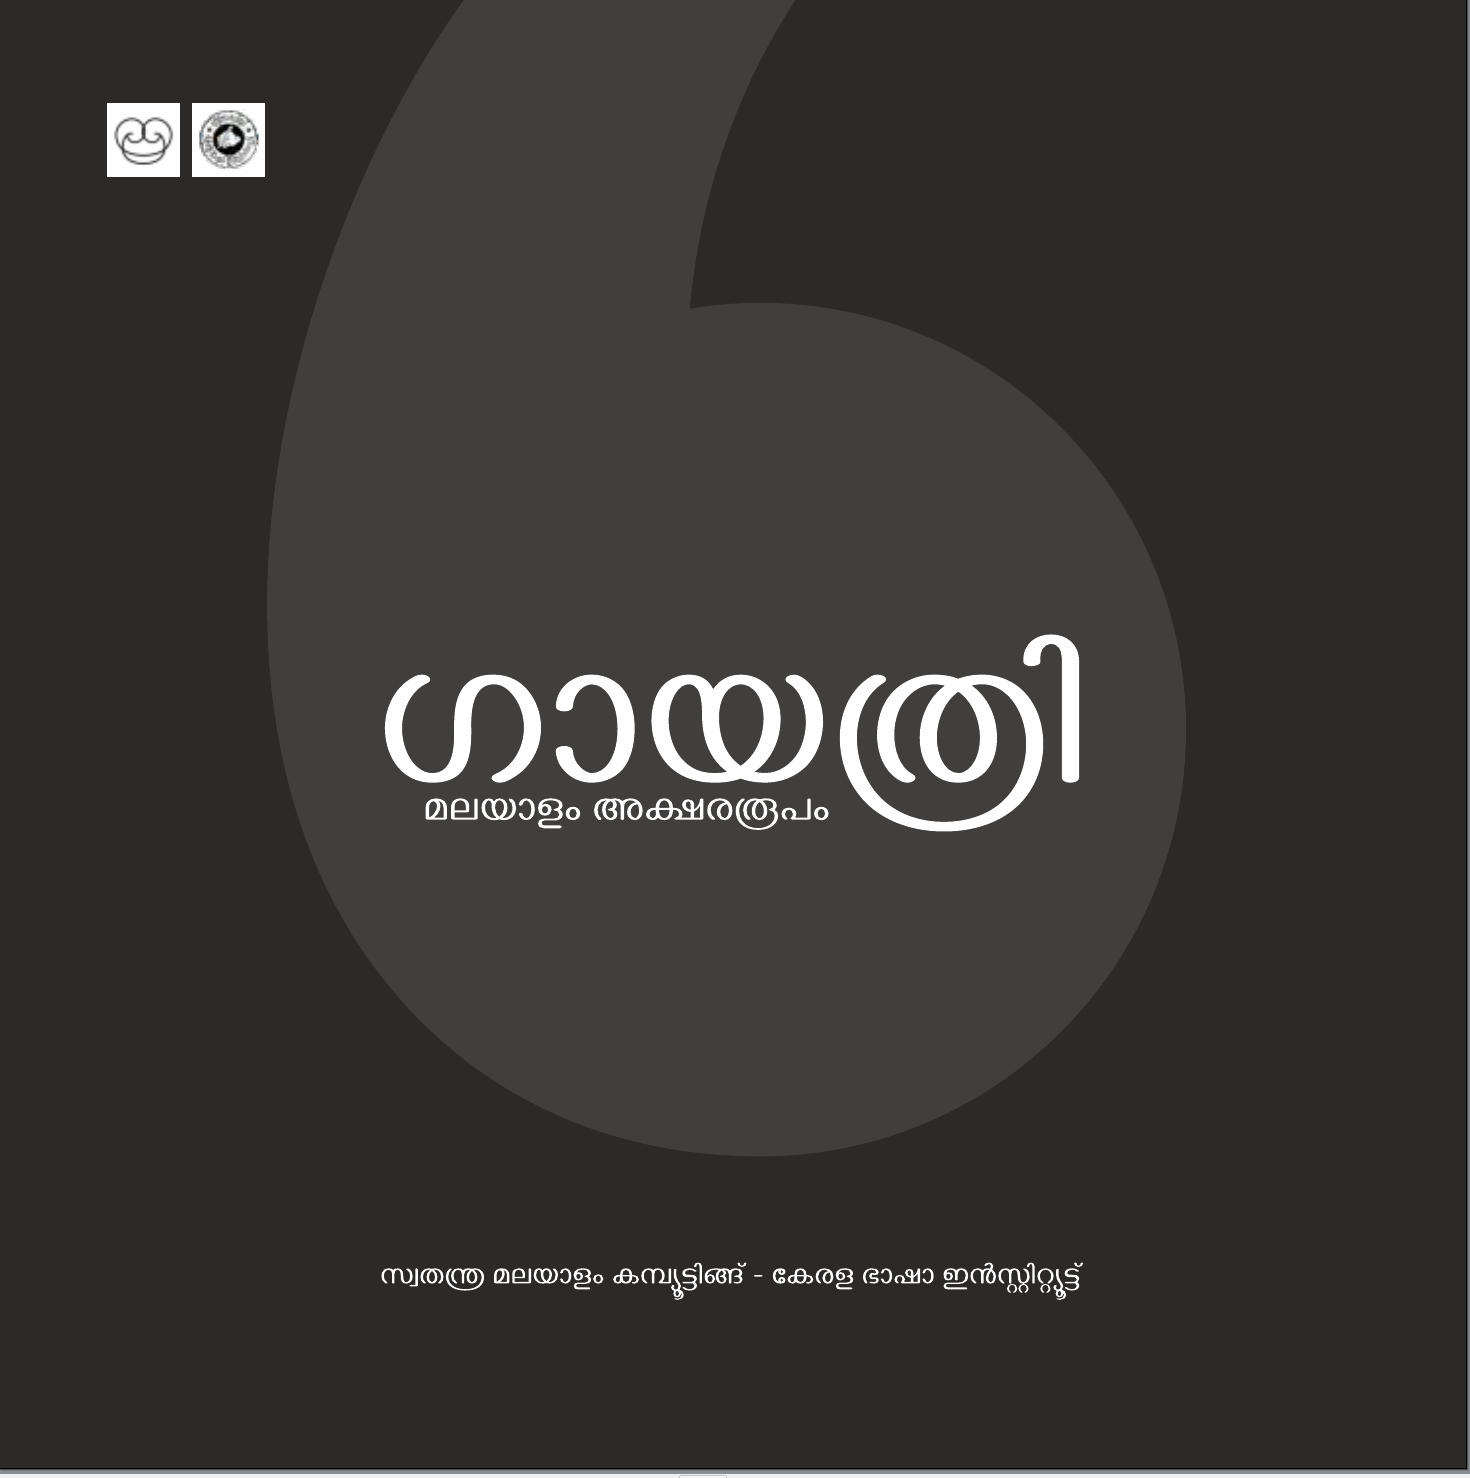
\includegraphics[width=\paperwidth]{title.png}
  }%
}

\begin{document}
	
\begin{titlepage}
\BgThispage
\centering
\vfill
{{\Large { ‌ }}}
\vfill
{{\Large {പ്രോജക്ട് റിപ്പോർട്ട് }}}\\[.5cm]
{{\Large {നവമ്പർ 2018}}}\\
\end{titlepage}
 

\thispagestyle{empty}	
\clearpage
	
	\chapter*{ആമുഖം}
	

	കേരള ഭാഷാ ഇന്‍സ്റ്റിറ്റ്യൂട്ടിന്റെ സാമ്പത്തികസഹായത്തോടെ സ്വതന്ത്ര മലയാളം കമ്പ്യൂട്ടിങ്ങ് രൂപകല്പന ചെയ്തു പുറത്തിറക്കിയ മലയാളം യൂണിക്കോഡ് അക്ഷരരൂപമാണ്  \textbf{ഗായത്രി}. അക്ഷരങ്ങളുടെ  രൂപകല്പന നിർവഹിച്ചത് ശ്രീ. ബിനോയ് ഡൊമിനിക്ക് ആണ്. ഓപ്പണ്‍ടൈപ്പ് സാങ്കേതികതയിൽ കാവ്യ മനോഹർ പ്രവർത്തിച്ചു. പ്രോജക്ട് മേല്‍നോട്ടം സന്തോഷ് തോട്ടിങ്ങൽ നിർവ്വഹിച്ചു.
	
	\paragraph{}
	റെഗുലര്‍, ബോള്‍ഡ്, തിന്‍ എന്നിങ്ങനെ മൂന്നു കനങ്ങളിലുള്ള ഫോണ്ടുകളായി ലഭ്യമായ ഗായത്രി, തലക്കെട്ടുകള്‍ക്ക് അനുയോജ്യമായ വിധമാണ് രൂപകല്പന ചെയ്തിരിക്കുന്നത്. എങ്കിലും ചെറിയ വലിപ്പത്തിലും സാമാന്യം നല്ല വായനാക്ഷമത ഗായത്രിയ്ക്കുണ്ട്. ഈ റിപ്പോര്‍ട്ട് പൂര്‍ണ്ണമായും ഗായത്രി  ഉപയോഗിച്ചാണ് തയ്യാറാക്കിയിരിക്കുന്നത്.
	\paragraph{}
	മെച്ചപ്പെട്ട മലയാളം ഫോണ്ടുകളുടെ ലഭ്യത മലയാളത്തിൽ കുറവാണ്. സ്വതന്ത്ര മലയാളം കമ്പ്യൂട്ടിങ്ങിന്റെ സാങ്കേതികമികവിൽ പുറത്തിറക്കിയ  മലയാളം ഫോണ്ടുകളുടെ കൂടെ ഗായത്രി എന്ന ഈ അക്ഷരരൂപം കൂടി സമർപ്പിക്കുന്നു.
\thispagestyle{empty}
\clearpage
	\chapter*{ അക്ഷരസഞ്ചയം}
	

	
	യൂണിക്കോഡിന്റെ പതിനൊന്നാം പതിപ്പിനെ ആധാരമാക്കിയാണ് ഗായത്രി നിര്‍മ്മിച്ചിട്ടുള്ളത്. മലയാളത്തില്‍ ഇന്ന് നിത്യോപയോഗത്തിലുള്ള സ്വരങ്ങളും വ്യഞ്ജനങ്ങളും ചില്ലക്ഷരങ്ങളും അക്കങ്ങളും കൂടാതെ പ്രാചീനമലയാളത്തില്‍ നിലനിന്നിരുന്ന അക്ഷരങ്ങളും അക്കങ്ങളുമെല്ലാം ചേര്‍ന്ന സമഗ്രമായ അക്ഷരസഞ്ചയം ഗായത്രിയിലുണ്ട്. മലയാളത്തിലെ പുരാരേഖകള്‍ ഡിജിറ്റൈസ് ചെയ്യുമ്പോള്‍ അത്യന്താപേക്ഷിതമാണിവ. കാല്‍, അര, മുക്കാല്‍, പതിനാറില്‍മൂന്ന് തുടങ്ങിയ ഭിന്നസംഖ്യാരൂപങ്ങളെ കുറിക്കുന്ന ൳, ൴, ൵, ൸ ചിഹ്നങ്ങളൊക്കെ ഗായത്രിയിലുണ്ട്. മലയാളം യൂണിക്കോഡ് പട്ടിക സമ്പൂർണ്ണമായി ഗായത്രിയിൽ തയ്യാറാക്കിയിരിക്കുന്നത് ചിത്രം \ref{unicode} ല്‍ കാണാം.
	
	\begin{figure}
		\begin{centering}
			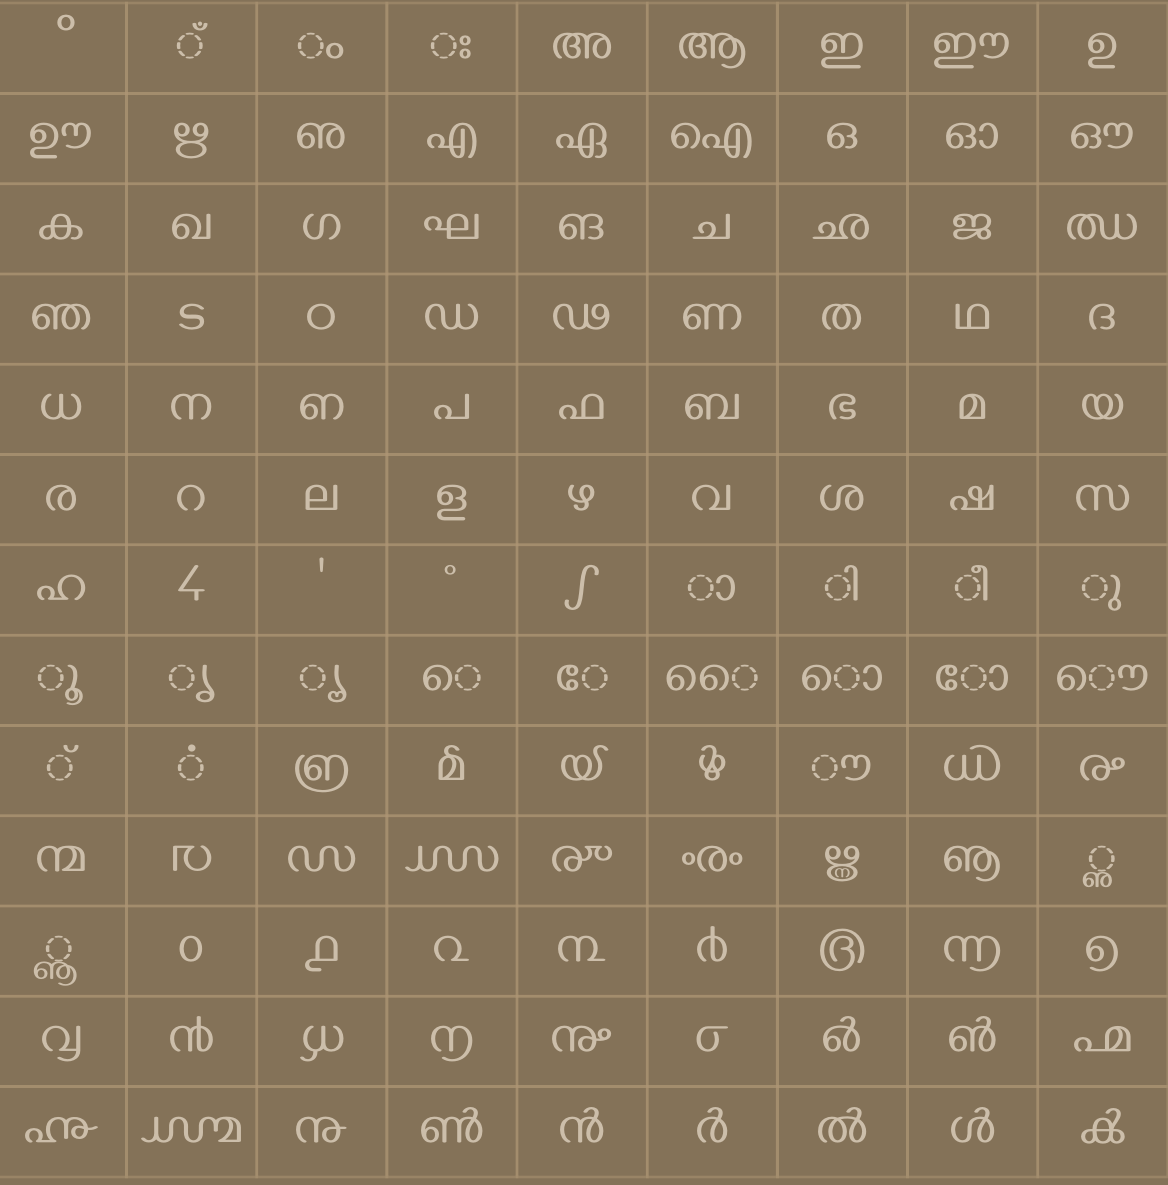
\includegraphics[width=0.8\textwidth]{ml-unicode.png}
			\caption{മലയാളം യൂണിക്കോഡ് സമ്പൂര്‍ണ്ണ കവറേജ്}
			\label{unicode}
		\end{centering}
	\end{figure}
	
	\paragraph{}
	മലയാളത്തിലെ കൂട്ടക്ഷരങ്ങളെ പരമാവധി ഉള്‍ക്കൊള്ളിച്ചുകൊണ്ടാണ് ഗായത്രിയുടെ രൂപകല്പന‍. അതുകൊണ്ട് തന്നെ ഇതിനെ ഒരു സമഗ്രലിപി ഫോണ്ടെന്ന് വിളിക്കാം.
	
	\paragraph{}
	ഇന്ന് മലയാളരേഖകളില്‍ മലയാളത്തോടൊപ്പം ഇംഗ്ലീഷ് വാക്കുകളും കലര്‍ത്തിയെഴുതുന്നത് സര്‍വ്വ സാധാരണമാണ്. അതുകൊണ്ട് തന്നെ ആധുനികമലയാളം ഫോണ്ടുകളില്‍ മലയാളം ലിപിയുടെ ശൈലിയ്ക്ക് അനുരൂപമായ ഇംഗ്ലീഷുള്‍പ്പെടുന്ന ലാറ്റിന്‍ അക്ഷരങ്ങളും അത്യാവശ്യമാണ്. ഗായത്രിയിൽ ലാറ്റിന്‍ അക്ഷരങ്ങളും കൂടി അതുകൊണ്ടു തന്നെ ഉള്‍പ്പെടുത്തിയിട്ടുണ്ട്.  എല്ലാം ചേര്‍ന്ന് ആകെ ആയിരത്തി ഒരുന്നൂറിൽപ്പരം അക്ഷരരൂപങ്ങൾ‍ ഗായത്രിയിലുണ്ട്. 
	
	\paragraph{}
	മലയാളത്തിലെ ചില അക്ഷരങ്ങള്‍ക്ക് സാര്‍വ്വത്രികമായി ഒരേ രൂപമല്ല ഉള്ളത്. 'ച്ച', 'കൂ', 'ള്ള' തുടങ്ങിയവയുടെ ശൈലീഭേദങ്ങളുള്‍ക്കൊണ്ടുകൊണ്ട് അവ കൂടി ഗായത്രിയിൽ ചേര്‍ത്തിട്ടുണ്ട്. സോഫ്റ്റ്‌വെയര്‍ സഹായത്തോടെ ഇതിലേതുവേണമെന്നു തെരഞ്ഞെടുക്കാന്‍ ഉപയോക്താവിനാകും. ചിത്രം \ref{style} കാണുക. 
	‍ 
	\begin{figure}
		\begin{centering}
			
\includegraphics[width=0.8\textwidth]{style.jpg}
			\caption{കൂ, ച്ച, ള്ള എന്നിവയുടെ ശൈലീഭേദങ്ങൾ ചിത്രീകരിച്ചിരിക്കുന്നു.}
			\label{style}
		\end{centering}
	\end{figure}
	
	
	\chapter*{രൂപകല്പന}
	
	ആമുഖത്തില്‍ സൂചിപ്പിച്ചത് പോലെ തലക്കെട്ടുകള്‍ക്ക് അനുയോജ്യമായ വിധമാണ് ഗായത്രിയുടെ രൂപകല്പന‍. അക്ഷരങ്ങളിലെ വരകൾക്ക് ഒരേ വീതിയല്ല. അക്ഷരങ്ങളുടെ അറ്റങ്ങള്‍ ഏതാണ്ട് ഉരുണ്ടിട്ടാണ്. കൂർത്ത അറ്റങ്ങൾ ഇല്ലാത്തതുകൊണ്ട് വായന ആയാസരഹിതമായി നടക്കുകയും ചെയ്യും.  വലിയ രൂപത്തില്‍ ഇവ വ്യക്തമായി കാണാവുന്ന മിഴിവാര്‍ന്ന ഡിസൈന്‍ സാദ്ധ്യതകള്‍ ഗായത്രിയ്ക്ക് നല്‍കാനാകും.  ചിത്രം \ref{one} നോക്കുക.
	
	\begin{figure}
		\begin{centering}
			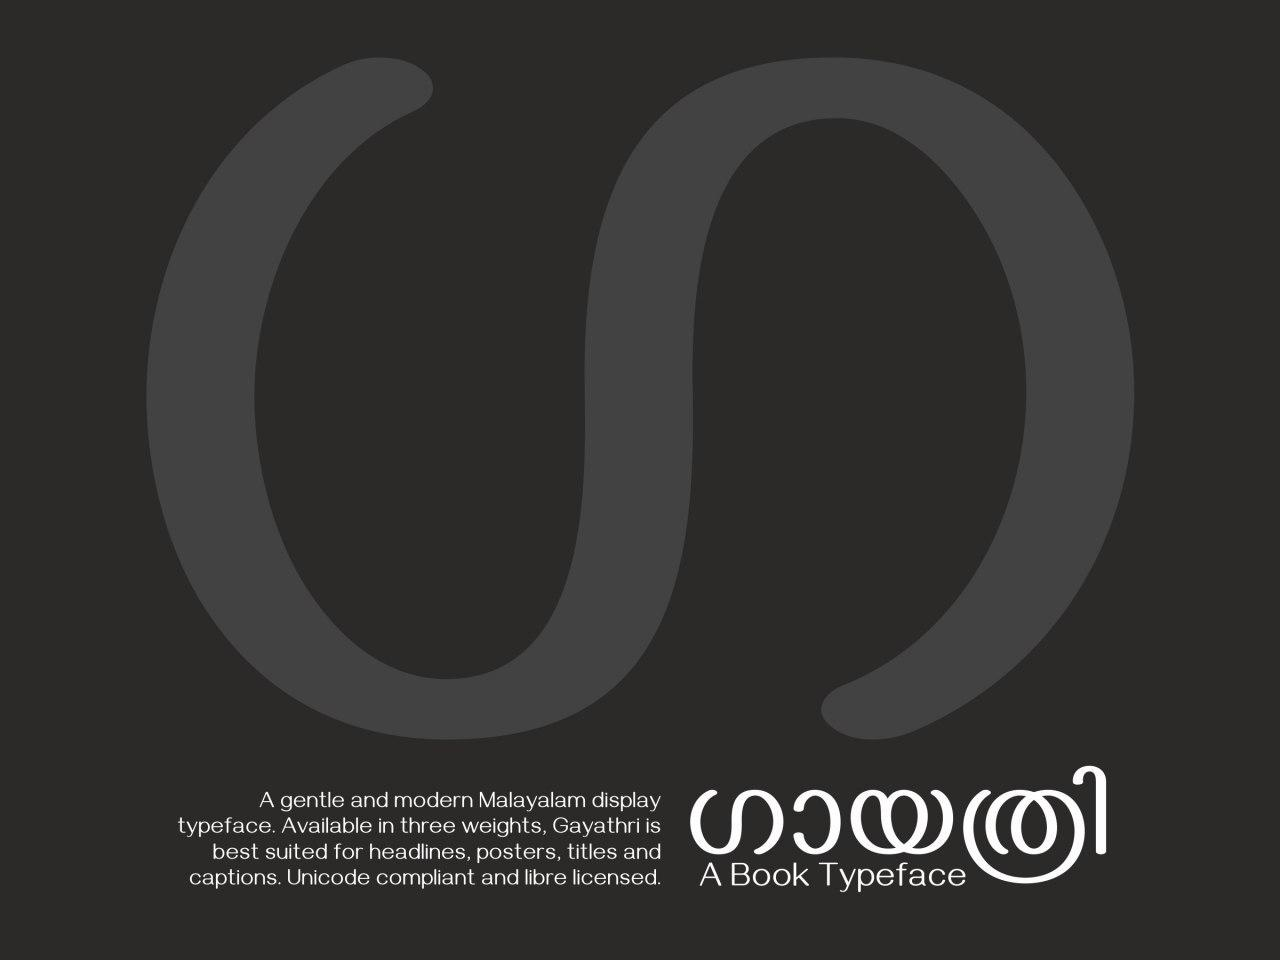
\includegraphics[width=0.8\textwidth]{ga.jpg}
			\caption{ഡിസൈന്‍ വിശദാംശങ്ങള്‍. അക്ഷരങ്ങളുടെ അറ്റങ്ങൾ ഉരുണ്ടതും വായനാസുഖം നൽകുന്നതുമാണ്.}
			\label{one}
		\end{centering}
	\end{figure}
	
	\paragraph{}
	പുസ്തകങ്ങളുടേയും ആനുകാലികങ്ങളുടേയുമെല്ലാം ലേയൗട്ട് തയ്യാറാക്കുമ്പോള്‍ പല കനത്തിലുള്ള ഫോണ്ട് വേരിയന്റുകള്‍ ആവശ്യമായി വരാറുണ്ട്. ഇതിനായി മൂന്നുകനങ്ങളില്‍ - ബോള്‍ഡ്, റെഗുലര്‍, തിന്‍- ഗായത്രി അക്ഷരരൂപങ്ങള്‍ ലഭ്യമാണ്. 
	
	\chapter*{നിര്‍മ്മാണവും ലൈസന്‍സിങ്ങും}
	
	ഗായത്രി ഫോണ്ട് നിര്‍മ്മാണം പൂര്‍ണ്ണമായും സ്വതന്ത്രസോഫ്റ്റ്‌വെയർ ഉപയോഗിച്ചാണ് നിർമ്മിച്ചിരിക്കുന്നത്. ഡിസൈനര്‍ അക്ഷരങ്ങളുടെ ബോള്‍ഡ്, റെഗുലര്‍, തിന്‍ ശൈലികളിലുള്ള വെക്ടര്‍ ഇമേജുകള്‍ തയ്യാറാക്കി. ഫോണ്ടിന്റെ മൂലരൂപം UFO (Unified Font Object) ഫോര്‍മാറ്റിലാണ്. അക്ഷരങ്ങളുടെ വെക്ടർ ചിത്രങ്ങളെ UFO മാതൃകയിലുള്ള ഗ്ലിഫ് ഫയലുകള്‍ ആക്കുകയാണ് ഫോണ്ട് എഞ്ചിനീയറിങ്ങിലെ ആദ്യ പടിയായി ചെയ്തത്. പിന്നീട് കൂട്ടക്ഷരങ്ങള്‍ കൃത്യമായി ചിത്രീകരിക്കാനാവശ്യമായ ഓപ്പണ്‍ടൈപ്പ് നിയമങ്ങള്‍ ചേര്‍ത്ത്  OTF, TTF, WOFF ഫോര്‍മറ്റിലുള്ള ഫോണ്ടുകള്‍ നിര്‍മ്മിച്ചു. ഈ ഫോര്‍മാറ്റുകളിലെല്ലാമുള്ള ഗായത്രിയുടെ ബോള്‍ഡ്, റെഗുലര്‍, തിന്‍ ഫോണ്ടുകള്‍ സ്വതന്ത്ര മലയാളം കമ്പ്യൂട്ടിങ്ങിന്റെ (\url{https://smc.org.in/fonts/}) വെബ്സൈറ്റിൽ നിന്നും ഡൗണ്‍ലോഡ് ചെയ്യാന്‍ ലഭ്യമാണ്.
	
	\paragraph{}
	ഫോണ്ടിന്റെ സോഴ്സ് കോഡ് സ്വതന്ത്രമാണ്. അതായത്, വരച്ച അക്ഷരരൂപങ്ങളുടെ വെക്ടര്‍ ഇമേജുകള്‍ (svg format), ഇവയില്‍ നിന്നും തയ്യാറാക്കിയ ഗ്ലിഫ് ഫയലുകള്‍, ഓപ്പണ്‍ടൈപ്പ്  നിയമങ്ങള്‍ ഇവയെല്ലാം നിര്‍മ്മാണഘട്ടത്തില്‍ ഇതുവരെ വരുത്തിയ മാറ്റങ്ങളുള്‍പ്പെടെ ഇവിടെ (\url{https://gitlab.com/smc/fonts/gayathri/}) ലഭ്യമാണ്.
	
	\paragraph{}
		ഓപ്പണ്‍ ഫോണ്ട് ലൈസന്‍സിലാണ് ഗായത്രി ഫോണ്ട് പുറത്തിറക്കിയിരിക്കുന്നത്.  കേരള ഭാഷാ ഇൻസ്റ്റിറ്റ്യൂട്ടിന്റെ സമ്പത്തിക സഹായത്തോടെയാണ്  സ്വതന്ത്ര മലയാളം കമ്പ്യൂട്ടിങ്ങ് ഗായത്രിയുടെ നിർമ്മാണം നിർവ്വഹിച്ചത്.
	
	\newpage
	\clearpage
	
	\chapter*{ഉപയോഗ മാതൃകകള്‍‍}
	
	ഗായത്രിയിൽ തയ്യാറാക്കിയ ചില താളുകൾ കാണാം. തലക്കെട്ടിൽ, ബ്ലർബിൽ, റെഗുലർ ടെക്‌സ്റ്റിൽ എല്ലാം ഗായത്രിയുടെ പല കനങ്ങളിലുള്ള  ഫോണ്ട് ഉപയോഗിച്ചിരിക്കുന്നു.

	\includepdf[pages=2-8]{usecase.pdf}
	
	
	\chapter*{സാങ്കേതിക വിശദാംശങ്ങള്‍}
	
	ഗായത്രി ഫോണ്ടില്‍ ഉള്‍ക്കൊള്ളിച്ചിട്ടുള്ള മുഴുവന്‍ അക്ഷരങ്ങളേയും കുറിച്ചുള്ള വിശദാംശങ്ങൾ 
	\\[1cm]

    \begin{tabular}[l]{|l|r|}
    \hline
  Unicode characters & 384 \\
Glyphs & 1124 \\
Ligature glyphs & 466 \\
Mark glyphs & 2 \\\hline
\end{tabular}

	
  
    \newfontface\customfont[Path= ../build/, Color =0000AA]{Gayathri-Regular.ttf}

  \title{Gayathri Regular}
\author{Binoy Dominic <binoy.domenic@gmail.com> (SMC)}
\renewcommand\today{Version 1.000}
%\maketitle

\section{Block}

    \newcommand\cell[2]{\begin{tabular}[c]{@{}c@{}}
      \customfont{\symbol{#1}}\\ \tiny{#2}\end{tabular}}
  
    \subsection{0000 - 00FF}
    \begin{tabular}{r|c|c|c|c|c|c|c|c|c|c|c|c|c|c|c|c|}
  &\multicolumn{1}{c}{000} & \multicolumn{1}{c}{001} & \multicolumn{1}{c}{002} & \multicolumn{1}{c}{003} & \multicolumn{1}{c}{004} & \multicolumn{1}{c}{005} & \multicolumn{1}{c}{006} & \multicolumn{1}{c}{007} & \multicolumn{1}{c}{008} & \multicolumn{1}{c}{009} & \multicolumn{1}{c}{00A} & \multicolumn{1}{c}{00B} & \multicolumn{1}{c}{00C} & \multicolumn{1}{c}{00D} & \multicolumn{1}{c}{00E} & \multicolumn{1}{c|}{00F}\\
\cline{2-17}
\small{0} & \cellcolor{gray}{\cell{0}{0000}} & \cellcolor{gray}{\cell{0}{0010}} & \cell{32}{0020} & \cell{48}{0030} & \cell{64}{0040} & \cell{80}{0050} & \cell{96}{0060} & \cell{112}{0070} & \cellcolor{gray}{\cell{0}{0080}} & \cellcolor{gray}{\cell{0}{0090}} & \cell{160}{00A0} & \cell{176}{00B0} & \cell{192}{00C0} & \cell{208}{00D0} & \cell{224}{00E0} & \cell{240}{00F0}\\
\cline{2-17}
\small{1} & \cellcolor{gray}{\cell{0}{0001}} & \cellcolor{gray}{\cell{0}{0011}} & \cell{33}{0021} & \cell{49}{0031} & \cell{65}{0041} & \cell{81}{0051} & \cell{97}{0061} & \cell{113}{0071} & \cellcolor{gray}{\cell{0}{0081}} & \cellcolor{gray}{\cell{0}{0091}} & \cellcolor{gray}{\cell{0}{00A1}} & \cellcolor{gray}{\cell{0}{00B1}} & \cell{193}{00C1} & \cell{209}{00D1} & \cell{225}{00E1} & \cell{241}{00F1}\\
\cline{2-17}
\small{2} & \cellcolor{gray}{\cell{0}{0002}} & \cellcolor{gray}{\cell{0}{0012}} & \cell{34}{0022} & \cell{50}{0032} & \cell{66}{0042} & \cell{82}{0052} & \cell{98}{0062} & \cell{114}{0072} & \cellcolor{gray}{\cell{0}{0082}} & \cellcolor{gray}{\cell{0}{0092}} & \cellcolor{gray}{\cell{0}{00A2}} & \cell{178}{00B2} & \cell{194}{00C2} & \cell{210}{00D2} & \cell{226}{00E2} & \cell{242}{00F2}\\
\cline{2-17}
\small{3} & \cellcolor{gray}{\cell{0}{0003}} & \cellcolor{gray}{\cell{0}{0013}} & \cell{35}{0023} & \cell{51}{0033} & \cell{67}{0043} & \cell{83}{0053} & \cell{99}{0063} & \cell{115}{0073} & \cellcolor{gray}{\cell{0}{0083}} & \cellcolor{gray}{\cell{0}{0093}} & \cell{163}{00A3} & \cell{179}{00B3} & \cell{195}{00C3} & \cell{211}{00D3} & \cell{227}{00E3} & \cell{243}{00F3}\\
\cline{2-17}
\small{4} & \cellcolor{gray}{\cell{0}{0004}} & \cellcolor{gray}{\cell{0}{0014}} & \cell{36}{0024} & \cell{52}{0034} & \cell{68}{0044} & \cell{84}{0054} & \cell{100}{0064} & \cell{116}{0074} & \cellcolor{gray}{\cell{0}{0084}} & \cellcolor{gray}{\cell{0}{0094}} & \cellcolor{gray}{\cell{0}{00A4}} & \cell{180}{00B4} & \cell{196}{00C4} & \cell{212}{00D4} & \cell{228}{00E4} & \cell{244}{00F4}\\
\cline{2-17}
\small{5} & \cellcolor{gray}{\cell{0}{0005}} & \cellcolor{gray}{\cell{0}{0015}} & \cell{37}{0025} & \cell{53}{0035} & \cell{69}{0045} & \cell{85}{0055} & \cell{101}{0065} & \cell{117}{0075} & \cellcolor{gray}{\cell{0}{0085}} & \cellcolor{gray}{\cell{0}{0095}} & \cell{165}{00A5} & \cellcolor{gray}{\cell{0}{00B5}} & \cell{197}{00C5} & \cell{213}{00D5} & \cell{229}{00E5} & \cell{245}{00F5}\\
\cline{2-17}
\small{6} & \cellcolor{gray}{\cell{0}{0006}} & \cellcolor{gray}{\cell{0}{0016}} & \cell{38}{0026} & \cell{54}{0036} & \cell{70}{0046} & \cell{86}{0056} & \cell{102}{0066} & \cell{118}{0076} & \cellcolor{gray}{\cell{0}{0086}} & \cellcolor{gray}{\cell{0}{0096}} & \cellcolor{gray}{\cell{0}{00A6}} & \cell{182}{00B6} & \cell{198}{00C6} & \cell{214}{00D6} & \cell{230}{00E6} & \cell{246}{00F6}\\
\cline{2-17}
\small{7} & \cellcolor{gray}{\cell{0}{0007}} & \cellcolor{gray}{\cell{0}{0017}} & \cell{39}{0027} & \cell{55}{0037} & \cell{71}{0047} & \cell{87}{0057} & \cell{103}{0067} & \cell{119}{0077} & \cellcolor{gray}{\cell{0}{0087}} & \cellcolor{gray}{\cell{0}{0097}} & \cellcolor{gray}{\cell{0}{00A7}} & \cellcolor{gray}{\cell{0}{00B7}} & \cell{199}{00C7} & \cell{215}{00D7} & \cell{231}{00E7} & \cell{247}{00F7}\\
\cline{2-17}
\small{8} & \cellcolor{gray}{\cell{0}{0008}} & \cellcolor{gray}{\cell{0}{0018}} & \cell{40}{0028} & \cell{56}{0038} & \cell{72}{0048} & \cell{88}{0058} & \cell{104}{0068} & \cell{120}{0078} & \cellcolor{gray}{\cell{0}{0088}} & \cellcolor{gray}{\cell{0}{0098}} & \cell{168}{00A8} & \cell{184}{00B8} & \cell{200}{00C8} & \cell{216}{00D8} & \cell{232}{00E8} & \cell{248}{00F8}\\
\cline{2-17}
\small{9} & \cellcolor{gray}{\cell{0}{0009}} & \cellcolor{gray}{\cell{0}{0019}} & \cell{41}{0029} & \cell{57}{0039} & \cell{73}{0049} & \cell{89}{0059} & \cell{105}{0069} & \cell{121}{0079} & \cellcolor{gray}{\cell{0}{0089}} & \cellcolor{gray}{\cell{0}{0099}} & \cell{169}{00A9} & \cell{185}{00B9} & \cell{201}{00C9} & \cell{217}{00D9} & \cell{233}{00E9} & \cell{249}{00F9}\\
\cline{2-17}
\small{A} & \cellcolor{gray}{\cell{0}{000A}} & \cellcolor{gray}{\cell{0}{001A}} & \cell{42}{002A} & \cell{58}{003A} & \cell{74}{004A} & \cell{90}{005A} & \cell{106}{006A} & \cell{122}{007A} & \cellcolor{gray}{\cell{0}{008A}} & \cellcolor{gray}{\cell{0}{009A}} & \cellcolor{gray}{\cell{0}{00AA}} & \cellcolor{gray}{\cell{0}{00BA}} & \cell{202}{00CA} & \cell{218}{00DA} & \cell{234}{00EA} & \cell{250}{00FA}\\
\cline{2-17}
\small{B} & \cellcolor{gray}{\cell{0}{000B}} & \cellcolor{gray}{\cell{0}{001B}} & \cell{43}{002B} & \cell{59}{003B} & \cell{75}{004B} & \cell{91}{005B} & \cell{107}{006B} & \cell{123}{007B} & \cellcolor{gray}{\cell{0}{008B}} & \cellcolor{gray}{\cell{0}{009B}} & \cell{171}{00AB} & \cell{187}{00BB} & \cell{203}{00CB} & \cell{219}{00DB} & \cell{235}{00EB} & \cell{251}{00FB}\\
\cline{2-17}
\small{C} & \cellcolor{gray}{\cell{0}{000C}} & \cellcolor{gray}{\cell{0}{001C}} & \cell{44}{002C} & \cell{60}{003C} & \cell{76}{004C} & \cell{92}{005C} & \cell{108}{006C} & \cell{124}{007C} & \cellcolor{gray}{\cell{0}{008C}} & \cellcolor{gray}{\cell{0}{009C}} & \cellcolor{gray}{\cell{0}{00AC}} & \cellcolor{gray}{\cell{0}{00BC}} & \cell{204}{00CC} & \cell{220}{00DC} & \cell{236}{00EC} & \cell{252}{00FC}\\
\cline{2-17}
\small{D} & \cellcolor{gray}{\cell{0}{000D}} & \cellcolor{gray}{\cell{0}{001D}} & \cell{45}{002D} & \cell{61}{003D} & \cell{77}{004D} & \cell{93}{005D} & \cell{109}{006D} & \cell{125}{007D} & \cellcolor{gray}{\cell{0}{008D}} & \cellcolor{gray}{\cell{0}{009D}} & \cell{173}{00AD} & \cellcolor{gray}{\cell{0}{00BD}} & \cell{205}{00CD} & \cell{221}{00DD} & \cell{237}{00ED} & \cell{253}{00FD}\\
\cline{2-17}
\small{E} & \cellcolor{gray}{\cell{0}{000E}} & \cellcolor{gray}{\cell{0}{001E}} & \cell{46}{002E} & \cell{62}{003E} & \cell{78}{004E} & \cell{94}{005E} & \cell{110}{006E} & \cell{126}{007E} & \cellcolor{gray}{\cell{0}{008E}} & \cellcolor{gray}{\cell{0}{009E}} & \cell{174}{00AE} & \cellcolor{gray}{\cell{0}{00BE}} & \cell{206}{00CE} & \cell{222}{00DE} & \cell{238}{00EE} & \cell{254}{00FE}\\
\cline{2-17}
\small{F} & \cellcolor{gray}{\cell{0}{000F}} & \cellcolor{gray}{\cell{0}{001F}} & \cell{47}{002F} & \cell{63}{003F} & \cell{79}{004F} & \cell{95}{005F} & \cell{111}{006F} & \cellcolor{gray}{\cell{0}{007F}} & \cellcolor{gray}{\cell{0}{008F}} & \cellcolor{gray}{\cell{0}{009F}} & \cell{175}{00AF} & \cell{191}{00BF} & \cell{207}{00CF} & \cell{223}{00DF} & \cell{239}{00EF} & \cell{255}{00FF}\\
\cline{2-17}
\end{tabular}\pagebreak
    \subsection{0100 - 01FF}
    \begin{tabular}{r|c|c|c|c|c|c|c|c|c|c|c|c|c|c|c|c|}
  &\multicolumn{1}{c}{010} & \multicolumn{1}{c}{011} & \multicolumn{1}{c}{012} & \multicolumn{1}{c}{013} & \multicolumn{1}{c}{014} & \multicolumn{1}{c}{015} & \multicolumn{1}{c}{016} & \multicolumn{1}{c}{017} & \multicolumn{1}{c}{018} & \multicolumn{1}{c}{019} & \multicolumn{1}{c}{01A} & \multicolumn{1}{c}{01B} & \multicolumn{1}{c}{01C} & \multicolumn{1}{c}{01D} & \multicolumn{1}{c}{01E} & \multicolumn{1}{c|}{01F}\\
\cline{2-17}
\small{0} & \cell{256}{0100} & \cellcolor{gray}{\cell{0}{0110}} & \cell{288}{0120} & \cellcolor{gray}{\cell{0}{0130}} & \cellcolor{gray}{\cell{0}{0140}} & \cellcolor{gray}{\cell{0}{0150}} & \cell{352}{0160} & \cellcolor{gray}{\cell{0}{0170}} & \cellcolor{gray}{\cell{0}{0180}} & \cellcolor{gray}{\cell{0}{0190}} & \cellcolor{gray}{\cell{0}{01A0}} & \cellcolor{gray}{\cell{0}{01B0}} & \cellcolor{gray}{\cell{0}{01C0}} & \cellcolor{gray}{\cell{0}{01D0}} & \cellcolor{gray}{\cell{0}{01E0}} & \cellcolor{gray}{\cell{0}{01F0}}\\
\cline{2-17}
\small{1} & \cell{257}{0101} & \cellcolor{gray}{\cell{0}{0111}} & \cell{289}{0121} & \cell{305}{0131} & \cellcolor{gray}{\cell{0}{0141}} & \cellcolor{gray}{\cell{0}{0151}} & \cell{353}{0161} & \cellcolor{gray}{\cell{0}{0171}} & \cellcolor{gray}{\cell{0}{0181}} & \cellcolor{gray}{\cell{0}{0191}} & \cellcolor{gray}{\cell{0}{01A1}} & \cellcolor{gray}{\cell{0}{01B1}} & \cellcolor{gray}{\cell{0}{01C1}} & \cellcolor{gray}{\cell{0}{01D1}} & \cellcolor{gray}{\cell{0}{01E1}} & \cellcolor{gray}{\cell{0}{01F1}}\\
\cline{2-17}
\small{2} & \cellcolor{gray}{\cell{0}{0102}} & \cell{274}{0112} & \cellcolor{gray}{\cell{0}{0122}} & \cellcolor{gray}{\cell{0}{0132}} & \cellcolor{gray}{\cell{0}{0142}} & \cell{338}{0152} & \cellcolor{gray}{\cell{0}{0162}} & \cellcolor{gray}{\cell{0}{0172}} & \cellcolor{gray}{\cell{0}{0182}} & \cellcolor{gray}{\cell{0}{0192}} & \cellcolor{gray}{\cell{0}{01A2}} & \cellcolor{gray}{\cell{0}{01B2}} & \cellcolor{gray}{\cell{0}{01C2}} & \cell{466}{01D2} & \cellcolor{gray}{\cell{0}{01E2}} & \cellcolor{gray}{\cell{0}{01F2}}\\
\cline{2-17}
\small{3} & \cellcolor{gray}{\cell{0}{0103}} & \cell{275}{0113} & \cellcolor{gray}{\cell{0}{0123}} & \cellcolor{gray}{\cell{0}{0133}} & \cell{323}{0143} & \cell{339}{0153} & \cellcolor{gray}{\cell{0}{0163}} & \cellcolor{gray}{\cell{0}{0173}} & \cellcolor{gray}{\cell{0}{0183}} & \cellcolor{gray}{\cell{0}{0193}} & \cellcolor{gray}{\cell{0}{01A3}} & \cellcolor{gray}{\cell{0}{01B3}} & \cellcolor{gray}{\cell{0}{01C3}} & \cell{467}{01D3} & \cellcolor{gray}{\cell{0}{01E3}} & \cellcolor{gray}{\cell{0}{01F3}}\\
\cline{2-17}
\small{4} & \cellcolor{gray}{\cell{0}{0104}} & \cellcolor{gray}{\cell{0}{0114}} & \cell{292}{0124} & \cellcolor{gray}{\cell{0}{0134}} & \cell{324}{0144} & \cell{340}{0154} & \cellcolor{gray}{\cell{0}{0164}} & \cell{372}{0174} & \cellcolor{gray}{\cell{0}{0184}} & \cellcolor{gray}{\cell{0}{0194}} & \cellcolor{gray}{\cell{0}{01A4}} & \cellcolor{gray}{\cell{0}{01B4}} & \cellcolor{gray}{\cell{0}{01C4}} & \cell{468}{01D4} & \cellcolor{gray}{\cell{0}{01E4}} & \cellcolor{gray}{\cell{0}{01F4}}\\
\cline{2-17}
\small{5} & \cellcolor{gray}{\cell{0}{0105}} & \cellcolor{gray}{\cell{0}{0115}} & \cell{293}{0125} & \cellcolor{gray}{\cell{0}{0135}} & \cellcolor{gray}{\cell{0}{0145}} & \cell{341}{0155} & \cellcolor{gray}{\cell{0}{0165}} & \cell{373}{0175} & \cellcolor{gray}{\cell{0}{0185}} & \cellcolor{gray}{\cell{0}{0195}} & \cellcolor{gray}{\cell{0}{01A5}} & \cellcolor{gray}{\cell{0}{01B5}} & \cellcolor{gray}{\cell{0}{01C5}} & \cellcolor{gray}{\cell{0}{01D5}} & \cellcolor{gray}{\cell{0}{01E5}} & \cellcolor{gray}{\cell{0}{01F5}}\\
\cline{2-17}
\small{6} & \cell{262}{0106} & \cell{278}{0116} & \cellcolor{gray}{\cell{0}{0126}} & \cellcolor{gray}{\cell{0}{0136}} & \cellcolor{gray}{\cell{0}{0146}} & \cellcolor{gray}{\cell{0}{0156}} & \cellcolor{gray}{\cell{0}{0166}} & \cell{374}{0176} & \cellcolor{gray}{\cell{0}{0186}} & \cellcolor{gray}{\cell{0}{0196}} & \cellcolor{gray}{\cell{0}{01A6}} & \cellcolor{gray}{\cell{0}{01B6}} & \cellcolor{gray}{\cell{0}{01C6}} & \cellcolor{gray}{\cell{0}{01D6}} & \cellcolor{gray}{\cell{0}{01E6}} & \cellcolor{gray}{\cell{0}{01F6}}\\
\cline{2-17}
\small{7} & \cell{263}{0107} & \cell{279}{0117} & \cellcolor{gray}{\cell{0}{0127}} & \cellcolor{gray}{\cell{0}{0137}} & \cell{327}{0147} & \cellcolor{gray}{\cell{0}{0157}} & \cellcolor{gray}{\cell{0}{0167}} & \cell{375}{0177} & \cellcolor{gray}{\cell{0}{0187}} & \cellcolor{gray}{\cell{0}{0197}} & \cellcolor{gray}{\cell{0}{01A7}} & \cellcolor{gray}{\cell{0}{01B7}} & \cellcolor{gray}{\cell{0}{01C7}} & \cellcolor{gray}{\cell{0}{01D7}} & \cellcolor{gray}{\cell{0}{01E7}} & \cellcolor{gray}{\cell{0}{01F7}}\\
\cline{2-17}
\small{8} & \cell{264}{0108} & \cellcolor{gray}{\cell{0}{0118}} & \cell{296}{0128} & \cellcolor{gray}{\cell{0}{0138}} & \cell{328}{0148} & \cell{344}{0158} & \cell{360}{0168} & \cellcolor{gray}{\cell{0}{0178}} & \cellcolor{gray}{\cell{0}{0188}} & \cellcolor{gray}{\cell{0}{0198}} & \cellcolor{gray}{\cell{0}{01A8}} & \cellcolor{gray}{\cell{0}{01B8}} & \cellcolor{gray}{\cell{0}{01C8}} & \cellcolor{gray}{\cell{0}{01D8}} & \cellcolor{gray}{\cell{0}{01E8}} & \cellcolor{gray}{\cell{0}{01F8}}\\
\cline{2-17}
\small{9} & \cell{265}{0109} & \cellcolor{gray}{\cell{0}{0119}} & \cell{297}{0129} & \cellcolor{gray}{\cell{0}{0139}} & \cellcolor{gray}{\cell{0}{0149}} & \cell{345}{0159} & \cell{361}{0169} & \cellcolor{gray}{\cell{0}{0179}} & \cellcolor{gray}{\cell{0}{0189}} & \cellcolor{gray}{\cell{0}{0199}} & \cellcolor{gray}{\cell{0}{01A9}} & \cellcolor{gray}{\cell{0}{01B9}} & \cellcolor{gray}{\cell{0}{01C9}} & \cellcolor{gray}{\cell{0}{01D9}} & \cellcolor{gray}{\cell{0}{01E9}} & \cellcolor{gray}{\cell{0}{01F9}}\\
\cline{2-17}
\small{A} & \cell{266}{010A} & \cell{282}{011A} & \cell{298}{012A} & \cellcolor{gray}{\cell{0}{013A}} & \cellcolor{gray}{\cell{0}{014A}} & \cell{346}{015A} & \cell{362}{016A} & \cell{378}{017A} & \cellcolor{gray}{\cell{0}{018A}} & \cellcolor{gray}{\cell{0}{019A}} & \cellcolor{gray}{\cell{0}{01AA}} & \cellcolor{gray}{\cell{0}{01BA}} & \cellcolor{gray}{\cell{0}{01CA}} & \cellcolor{gray}{\cell{0}{01DA}} & \cellcolor{gray}{\cell{0}{01EA}} & \cellcolor{gray}{\cell{0}{01FA}}\\
\cline{2-17}
\small{B} & \cell{267}{010B} & \cell{283}{011B} & \cell{299}{012B} & \cellcolor{gray}{\cell{0}{013B}} & \cellcolor{gray}{\cell{0}{014B}} & \cell{347}{015B} & \cell{363}{016B} & \cell{379}{017B} & \cellcolor{gray}{\cell{0}{018B}} & \cellcolor{gray}{\cell{0}{019B}} & \cellcolor{gray}{\cell{0}{01AB}} & \cellcolor{gray}{\cell{0}{01BB}} & \cellcolor{gray}{\cell{0}{01CB}} & \cellcolor{gray}{\cell{0}{01DB}} & \cellcolor{gray}{\cell{0}{01EB}} & \cellcolor{gray}{\cell{0}{01FB}}\\
\cline{2-17}
\small{C} & \cell{268}{010C} & \cell{284}{011C} & \cellcolor{gray}{\cell{0}{012C}} & \cellcolor{gray}{\cell{0}{013C}} & \cell{332}{014C} & \cell{348}{015C} & \cellcolor{gray}{\cell{0}{016C}} & \cell{380}{017C} & \cellcolor{gray}{\cell{0}{018C}} & \cellcolor{gray}{\cell{0}{019C}} & \cellcolor{gray}{\cell{0}{01AC}} & \cellcolor{gray}{\cell{0}{01BC}} & \cellcolor{gray}{\cell{0}{01CC}} & \cellcolor{gray}{\cell{0}{01DC}} & \cellcolor{gray}{\cell{0}{01EC}} & \cell{508}{01FC}\\
\cline{2-17}
\small{D} & \cell{269}{010D} & \cell{285}{011D} & \cellcolor{gray}{\cell{0}{012D}} & \cellcolor{gray}{\cell{0}{013D}} & \cell{333}{014D} & \cell{349}{015D} & \cellcolor{gray}{\cell{0}{016D}} & \cell{381}{017D} & \cellcolor{gray}{\cell{0}{018D}} & \cellcolor{gray}{\cell{0}{019D}} & \cellcolor{gray}{\cell{0}{01AD}} & \cellcolor{gray}{\cell{0}{01BD}} & \cellcolor{gray}{\cell{0}{01CD}} & \cellcolor{gray}{\cell{0}{01DD}} & \cellcolor{gray}{\cell{0}{01ED}} & \cell{509}{01FD}\\
\cline{2-17}
\small{E} & \cell{270}{010E} & \cellcolor{gray}{\cell{0}{011E}} & \cellcolor{gray}{\cell{0}{012E}} & \cellcolor{gray}{\cell{0}{013E}} & \cellcolor{gray}{\cell{0}{014E}} & \cell{350}{015E} & \cell{366}{016E} & \cell{382}{017E} & \cellcolor{gray}{\cell{0}{018E}} & \cellcolor{gray}{\cell{0}{019E}} & \cellcolor{gray}{\cell{0}{01AE}} & \cellcolor{gray}{\cell{0}{01BE}} & \cellcolor{gray}{\cell{0}{01CE}} & \cellcolor{gray}{\cell{0}{01DE}} & \cellcolor{gray}{\cell{0}{01EE}} & \cellcolor{gray}{\cell{0}{01FE}}\\
\cline{2-17}
\small{F} & \cellcolor{gray}{\cell{0}{010F}} & \cellcolor{gray}{\cell{0}{011F}} & \cellcolor{gray}{\cell{0}{012F}} & \cellcolor{gray}{\cell{0}{013F}} & \cellcolor{gray}{\cell{0}{014F}} & \cell{351}{015F} & \cell{367}{016F} & \cellcolor{gray}{\cell{0}{017F}} & \cellcolor{gray}{\cell{0}{018F}} & \cellcolor{gray}{\cell{0}{019F}} & \cellcolor{gray}{\cell{0}{01AF}} & \cellcolor{gray}{\cell{0}{01BF}} & \cellcolor{gray}{\cell{0}{01CF}} & \cellcolor{gray}{\cell{0}{01DF}} & \cellcolor{gray}{\cell{0}{01EF}} & \cellcolor{gray}{\cell{0}{01FF}}\\
\cline{2-17}
\end{tabular}\pagebreak
    \subsection{0D00 - 0DFF}
    \begin{tabular}{r|c|c|c|c|c|c|c|c|c|c|c|c|c|c|c|c|}
  &\multicolumn{1}{c}{0D0} & \multicolumn{1}{c}{0D1} & \multicolumn{1}{c}{0D2} & \multicolumn{1}{c}{0D3} & \multicolumn{1}{c}{0D4} & \multicolumn{1}{c}{0D5} & \multicolumn{1}{c}{0D6} & \multicolumn{1}{c}{0D7} & \multicolumn{1}{c}{0D8} & \multicolumn{1}{c}{0D9} & \multicolumn{1}{c}{0DA} & \multicolumn{1}{c}{0DB} & \multicolumn{1}{c}{0DC} & \multicolumn{1}{c}{0DD} & \multicolumn{1}{c}{0DE} & \multicolumn{1}{c|}{0DF}\\
\cline{2-17}
\small{0} & \cell{3328}{0D00} & \cell{3344}{0D10} & \cell{3360}{0D20} & \cell{3376}{0D30} & \cell{3392}{0D40} & \cellcolor{gray}{\cell{0}{0D50}} & \cell{3424}{0D60} & \cell{3440}{0D70} & \cellcolor{gray}{\cell{0}{0D80}} & \cellcolor{gray}{\cell{0}{0D90}} & \cellcolor{gray}{\cell{0}{0DA0}} & \cellcolor{gray}{\cell{0}{0DB0}} & \cellcolor{gray}{\cell{0}{0DC0}} & \cellcolor{gray}{\cell{0}{0DD0}} & \cellcolor{gray}{\cell{0}{0DE0}} & \cellcolor{gray}{\cell{0}{0DF0}}\\
\cline{2-17}
\small{1} & \cell{3329}{0D01} & \cellcolor{gray}{\cell{0}{0D11}} & \cell{3361}{0D21} & \cell{3377}{0D31} & \cell{3393}{0D41} & \cellcolor{gray}{\cell{0}{0D51}} & \cell{3425}{0D61} & \cell{3441}{0D71} & \cellcolor{gray}{\cell{0}{0D81}} & \cellcolor{gray}{\cell{0}{0D91}} & \cellcolor{gray}{\cell{0}{0DA1}} & \cellcolor{gray}{\cell{0}{0DB1}} & \cellcolor{gray}{\cell{0}{0DC1}} & \cellcolor{gray}{\cell{0}{0DD1}} & \cellcolor{gray}{\cell{0}{0DE1}} & \cellcolor{gray}{\cell{0}{0DF1}}\\
\cline{2-17}
\small{2} & \cell{3330}{0D02} & \cell{3346}{0D12} & \cell{3362}{0D22} & \cell{3378}{0D32} & \cell{3394}{0D42} & \cellcolor{gray}{\cell{0}{0D52}} & \cell{3426}{0D62} & \cell{3442}{0D72} & \cellcolor{gray}{\cell{0}{0D82}} & \cellcolor{gray}{\cell{0}{0D92}} & \cellcolor{gray}{\cell{0}{0DA2}} & \cellcolor{gray}{\cell{0}{0DB2}} & \cellcolor{gray}{\cell{0}{0DC2}} & \cellcolor{gray}{\cell{0}{0DD2}} & \cellcolor{gray}{\cell{0}{0DE2}} & \cellcolor{gray}{\cell{0}{0DF2}}\\
\cline{2-17}
\small{3} & \cell{3331}{0D03} & \cell{3347}{0D13} & \cell{3363}{0D23} & \cell{3379}{0D33} & \cell{3395}{0D43} & \cellcolor{gray}{\cell{0}{0D53}} & \cell{3427}{0D63} & \cell{3443}{0D73} & \cellcolor{gray}{\cell{0}{0D83}} & \cellcolor{gray}{\cell{0}{0D93}} & \cellcolor{gray}{\cell{0}{0DA3}} & \cellcolor{gray}{\cell{0}{0DB3}} & \cellcolor{gray}{\cell{0}{0DC3}} & \cellcolor{gray}{\cell{0}{0DD3}} & \cellcolor{gray}{\cell{0}{0DE3}} & \cellcolor{gray}{\cell{0}{0DF3}}\\
\cline{2-17}
\small{4} & \cellcolor{gray}{\cell{0}{0D04}} & \cell{3348}{0D14} & \cell{3364}{0D24} & \cell{3380}{0D34} & \cell{3396}{0D44} & \cell{3412}{0D54} & \cellcolor{gray}{\cell{0}{0D64}} & \cell{3444}{0D74} & \cellcolor{gray}{\cell{0}{0D84}} & \cellcolor{gray}{\cell{0}{0D94}} & \cellcolor{gray}{\cell{0}{0DA4}} & \cellcolor{gray}{\cell{0}{0DB4}} & \cellcolor{gray}{\cell{0}{0DC4}} & \cellcolor{gray}{\cell{0}{0DD4}} & \cellcolor{gray}{\cell{0}{0DE4}} & \cellcolor{gray}{\cell{0}{0DF4}}\\
\cline{2-17}
\small{5} & \cell{3333}{0D05} & \cell{3349}{0D15} & \cell{3365}{0D25} & \cell{3381}{0D35} & \cellcolor{gray}{\cell{0}{0D45}} & \cell{3413}{0D55} & \cellcolor{gray}{\cell{0}{0D65}} & \cell{3445}{0D75} & \cellcolor{gray}{\cell{0}{0D85}} & \cellcolor{gray}{\cell{0}{0D95}} & \cellcolor{gray}{\cell{0}{0DA5}} & \cellcolor{gray}{\cell{0}{0DB5}} & \cellcolor{gray}{\cell{0}{0DC5}} & \cellcolor{gray}{\cell{0}{0DD5}} & \cellcolor{gray}{\cell{0}{0DE5}} & \cellcolor{gray}{\cell{0}{0DF5}}\\
\cline{2-17}
\small{6} & \cell{3334}{0D06} & \cell{3350}{0D16} & \cell{3366}{0D26} & \cell{3382}{0D36} & \cell{3398}{0D46} & \cell{3414}{0D56} & \cell{3430}{0D66} & \cell{3446}{0D76} & \cellcolor{gray}{\cell{0}{0D86}} & \cellcolor{gray}{\cell{0}{0D96}} & \cellcolor{gray}{\cell{0}{0DA6}} & \cellcolor{gray}{\cell{0}{0DB6}} & \cellcolor{gray}{\cell{0}{0DC6}} & \cellcolor{gray}{\cell{0}{0DD6}} & \cellcolor{gray}{\cell{0}{0DE6}} & \cellcolor{gray}{\cell{0}{0DF6}}\\
\cline{2-17}
\small{7} & \cell{3335}{0D07} & \cell{3351}{0D17} & \cell{3367}{0D27} & \cell{3383}{0D37} & \cell{3399}{0D47} & \cell{3415}{0D57} & \cell{3431}{0D67} & \cell{3447}{0D77} & \cellcolor{gray}{\cell{0}{0D87}} & \cellcolor{gray}{\cell{0}{0D97}} & \cellcolor{gray}{\cell{0}{0DA7}} & \cellcolor{gray}{\cell{0}{0DB7}} & \cellcolor{gray}{\cell{0}{0DC7}} & \cellcolor{gray}{\cell{0}{0DD7}} & \cellcolor{gray}{\cell{0}{0DE7}} & \cellcolor{gray}{\cell{0}{0DF7}}\\
\cline{2-17}
\small{8} & \cell{3336}{0D08} & \cell{3352}{0D18} & \cell{3368}{0D28} & \cell{3384}{0D38} & \cell{3400}{0D48} & \cell{3416}{0D58} & \cell{3432}{0D68} & \cell{3448}{0D78} & \cellcolor{gray}{\cell{0}{0D88}} & \cellcolor{gray}{\cell{0}{0D98}} & \cellcolor{gray}{\cell{0}{0DA8}} & \cellcolor{gray}{\cell{0}{0DB8}} & \cellcolor{gray}{\cell{0}{0DC8}} & \cellcolor{gray}{\cell{0}{0DD8}} & \cellcolor{gray}{\cell{0}{0DE8}} & \cellcolor{gray}{\cell{0}{0DF8}}\\
\cline{2-17}
\small{9} & \cell{3337}{0D09} & \cell{3353}{0D19} & \cell{3369}{0D29} & \cell{3385}{0D39} & \cellcolor{gray}{\cell{0}{0D49}} & \cell{3417}{0D59} & \cell{3433}{0D69} & \cell{3449}{0D79} & \cellcolor{gray}{\cell{0}{0D89}} & \cellcolor{gray}{\cell{0}{0D99}} & \cellcolor{gray}{\cell{0}{0DA9}} & \cellcolor{gray}{\cell{0}{0DB9}} & \cellcolor{gray}{\cell{0}{0DC9}} & \cellcolor{gray}{\cell{0}{0DD9}} & \cellcolor{gray}{\cell{0}{0DE9}} & \cellcolor{gray}{\cell{0}{0DF9}}\\
\cline{2-17}
\small{A} & \cell{3338}{0D0A} & \cell{3354}{0D1A} & \cell{3370}{0D2A} & \cell{3386}{0D3A} & \cell{3402}{0D4A} & \cell{3418}{0D5A} & \cell{3434}{0D6A} & \cell{3450}{0D7A} & \cellcolor{gray}{\cell{0}{0D8A}} & \cellcolor{gray}{\cell{0}{0D9A}} & \cellcolor{gray}{\cell{0}{0DAA}} & \cellcolor{gray}{\cell{0}{0DBA}} & \cellcolor{gray}{\cell{0}{0DCA}} & \cellcolor{gray}{\cell{0}{0DDA}} & \cellcolor{gray}{\cell{0}{0DEA}} & \cellcolor{gray}{\cell{0}{0DFA}}\\
\cline{2-17}
\small{B} & \cell{3339}{0D0B} & \cell{3355}{0D1B} & \cell{3371}{0D2B} & \cell{3387}{0D3B} & \cell{3403}{0D4B} & \cell{3419}{0D5B} & \cell{3435}{0D6B} & \cell{3451}{0D7B} & \cellcolor{gray}{\cell{0}{0D8B}} & \cellcolor{gray}{\cell{0}{0D9B}} & \cellcolor{gray}{\cell{0}{0DAB}} & \cellcolor{gray}{\cell{0}{0DBB}} & \cellcolor{gray}{\cell{0}{0DCB}} & \cellcolor{gray}{\cell{0}{0DDB}} & \cellcolor{gray}{\cell{0}{0DEB}} & \cellcolor{gray}{\cell{0}{0DFB}}\\
\cline{2-17}
\small{C} & \cell{3340}{0D0C} & \cell{3356}{0D1C} & \cell{3372}{0D2C} & \cell{3388}{0D3C} & \cell{3404}{0D4C} & \cell{3420}{0D5C} & \cell{3436}{0D6C} & \cell{3452}{0D7C} & \cellcolor{gray}{\cell{0}{0D8C}} & \cellcolor{gray}{\cell{0}{0D9C}} & \cellcolor{gray}{\cell{0}{0DAC}} & \cellcolor{gray}{\cell{0}{0DBC}} & \cellcolor{gray}{\cell{0}{0DCC}} & \cellcolor{gray}{\cell{0}{0DDC}} & \cellcolor{gray}{\cell{0}{0DEC}} & \cellcolor{gray}{\cell{0}{0DFC}}\\
\cline{2-17}
\small{D} & \cellcolor{gray}{\cell{0}{0D0D}} & \cell{3357}{0D1D} & \cell{3373}{0D2D} & \cell{3389}{0D3D} & \cell{3405}{0D4D} & \cell{3421}{0D5D} & \cell{3437}{0D6D} & \cell{3453}{0D7D} & \cellcolor{gray}{\cell{0}{0D8D}} & \cellcolor{gray}{\cell{0}{0D9D}} & \cellcolor{gray}{\cell{0}{0DAD}} & \cellcolor{gray}{\cell{0}{0DBD}} & \cellcolor{gray}{\cell{0}{0DCD}} & \cellcolor{gray}{\cell{0}{0DDD}} & \cellcolor{gray}{\cell{0}{0DED}} & \cellcolor{gray}{\cell{0}{0DFD}}\\
\cline{2-17}
\small{E} & \cell{3342}{0D0E} & \cell{3358}{0D1E} & \cell{3374}{0D2E} & \cell{3390}{0D3E} & \cell{3406}{0D4E} & \cell{3422}{0D5E} & \cell{3438}{0D6E} & \cell{3454}{0D7E} & \cellcolor{gray}{\cell{0}{0D8E}} & \cellcolor{gray}{\cell{0}{0D9E}} & \cellcolor{gray}{\cell{0}{0DAE}} & \cellcolor{gray}{\cell{0}{0DBE}} & \cellcolor{gray}{\cell{0}{0DCE}} & \cellcolor{gray}{\cell{0}{0DDE}} & \cellcolor{gray}{\cell{0}{0DEE}} & \cellcolor{gray}{\cell{0}{0DFE}}\\
\cline{2-17}
\small{F} & \cell{3343}{0D0F} & \cell{3359}{0D1F} & \cell{3375}{0D2F} & \cell{3391}{0D3F} & \cell{3407}{0D4F} & \cell{3423}{0D5F} & \cell{3439}{0D6F} & \cell{3455}{0D7F} & \cellcolor{gray}{\cell{0}{0D8F}} & \cellcolor{gray}{\cell{0}{0D9F}} & \cellcolor{gray}{\cell{0}{0DAF}} & \cellcolor{gray}{\cell{0}{0DBF}} & \cellcolor{gray}{\cell{0}{0DCF}} & \cellcolor{gray}{\cell{0}{0DDF}} & \cellcolor{gray}{\cell{0}{0DEF}} & \cellcolor{gray}{\cell{0}{0DFF}}\\
\cline{2-17}
\end{tabular}\pagebreak
    \subsection{2000 - 20FF}
    \begin{tabular}{r|c|c|c|c|c|c|c|c|c|c|c|c|c|c|c|c|}
  &\multicolumn{1}{c}{200} & \multicolumn{1}{c}{201} & \multicolumn{1}{c}{202} & \multicolumn{1}{c}{203} & \multicolumn{1}{c}{204} & \multicolumn{1}{c}{205} & \multicolumn{1}{c}{206} & \multicolumn{1}{c}{207} & \multicolumn{1}{c}{208} & \multicolumn{1}{c}{209} & \multicolumn{1}{c}{20A} & \multicolumn{1}{c}{20B} & \multicolumn{1}{c}{20C} & \multicolumn{1}{c}{20D} & \multicolumn{1}{c}{20E} & \multicolumn{1}{c|}{20F}\\
\cline{2-17}
\small{0} & \cellcolor{gray}{\cell{0}{2000}} & \cellcolor{gray}{\cell{0}{2010}} & \cellcolor{gray}{\cell{0}{2020}} & \cellcolor{gray}{\cell{0}{2030}} & \cellcolor{gray}{\cell{0}{2040}} & \cellcolor{gray}{\cell{0}{2050}} & \cellcolor{gray}{\cell{0}{2060}} & \cell{8304}{2070} & \cellcolor{gray}{\cell{0}{2080}} & \cellcolor{gray}{\cell{0}{2090}} & \cellcolor{gray}{\cell{0}{20A0}} & \cellcolor{gray}{\cell{0}{20B0}} & \cellcolor{gray}{\cell{0}{20C0}} & \cellcolor{gray}{\cell{0}{20D0}} & \cellcolor{gray}{\cell{0}{20E0}} & \cellcolor{gray}{\cell{0}{20F0}}\\
\cline{2-17}
\small{1} & \cellcolor{gray}{\cell{0}{2001}} & \cellcolor{gray}{\cell{0}{2011}} & \cellcolor{gray}{\cell{0}{2021}} & \cellcolor{gray}{\cell{0}{2031}} & \cellcolor{gray}{\cell{0}{2041}} & \cellcolor{gray}{\cell{0}{2051}} & \cellcolor{gray}{\cell{0}{2061}} & \cellcolor{gray}{\cell{0}{2071}} & \cellcolor{gray}{\cell{0}{2081}} & \cellcolor{gray}{\cell{0}{2091}} & \cellcolor{gray}{\cell{0}{20A1}} & \cellcolor{gray}{\cell{0}{20B1}} & \cellcolor{gray}{\cell{0}{20C1}} & \cellcolor{gray}{\cell{0}{20D1}} & \cellcolor{gray}{\cell{0}{20E1}} & \cellcolor{gray}{\cell{0}{20F1}}\\
\cline{2-17}
\small{2} & \cellcolor{gray}{\cell{0}{2002}} & \cellcolor{gray}{\cell{0}{2012}} & \cell{8226}{2022} & \cellcolor{gray}{\cell{0}{2032}} & \cellcolor{gray}{\cell{0}{2042}} & \cellcolor{gray}{\cell{0}{2052}} & \cellcolor{gray}{\cell{0}{2062}} & \cellcolor{gray}{\cell{0}{2072}} & \cellcolor{gray}{\cell{0}{2082}} & \cellcolor{gray}{\cell{0}{2092}} & \cellcolor{gray}{\cell{0}{20A2}} & \cellcolor{gray}{\cell{0}{20B2}} & \cellcolor{gray}{\cell{0}{20C2}} & \cellcolor{gray}{\cell{0}{20D2}} & \cellcolor{gray}{\cell{0}{20E2}} & \cellcolor{gray}{\cell{0}{20F2}}\\
\cline{2-17}
\small{3} & \cellcolor{gray}{\cell{0}{2003}} & \cell{8211}{2013} & \cellcolor{gray}{\cell{0}{2023}} & \cellcolor{gray}{\cell{0}{2033}} & \cellcolor{gray}{\cell{0}{2043}} & \cellcolor{gray}{\cell{0}{2053}} & \cellcolor{gray}{\cell{0}{2063}} & \cellcolor{gray}{\cell{0}{2073}} & \cellcolor{gray}{\cell{0}{2083}} & \cellcolor{gray}{\cell{0}{2093}} & \cellcolor{gray}{\cell{0}{20A3}} & \cellcolor{gray}{\cell{0}{20B3}} & \cellcolor{gray}{\cell{0}{20C3}} & \cellcolor{gray}{\cell{0}{20D3}} & \cellcolor{gray}{\cell{0}{20E3}} & \cellcolor{gray}{\cell{0}{20F3}}\\
\cline{2-17}
\small{4} & \cellcolor{gray}{\cell{0}{2004}} & \cell{8212}{2014} & \cellcolor{gray}{\cell{0}{2024}} & \cellcolor{gray}{\cell{0}{2034}} & \cellcolor{gray}{\cell{0}{2044}} & \cellcolor{gray}{\cell{0}{2054}} & \cellcolor{gray}{\cell{0}{2064}} & \cell{8308}{2074} & \cellcolor{gray}{\cell{0}{2084}} & \cellcolor{gray}{\cell{0}{2094}} & \cellcolor{gray}{\cell{0}{20A4}} & \cellcolor{gray}{\cell{0}{20B4}} & \cellcolor{gray}{\cell{0}{20C4}} & \cellcolor{gray}{\cell{0}{20D4}} & \cellcolor{gray}{\cell{0}{20E4}} & \cellcolor{gray}{\cell{0}{20F4}}\\
\cline{2-17}
\small{5} & \cellcolor{gray}{\cell{0}{2005}} & \cellcolor{gray}{\cell{0}{2015}} & \cellcolor{gray}{\cell{0}{2025}} & \cellcolor{gray}{\cell{0}{2035}} & \cellcolor{gray}{\cell{0}{2045}} & \cellcolor{gray}{\cell{0}{2055}} & \cellcolor{gray}{\cell{0}{2065}} & \cell{8309}{2075} & \cellcolor{gray}{\cell{0}{2085}} & \cellcolor{gray}{\cell{0}{2095}} & \cellcolor{gray}{\cell{0}{20A5}} & \cellcolor{gray}{\cell{0}{20B5}} & \cellcolor{gray}{\cell{0}{20C5}} & \cellcolor{gray}{\cell{0}{20D5}} & \cellcolor{gray}{\cell{0}{20E5}} & \cellcolor{gray}{\cell{0}{20F5}}\\
\cline{2-17}
\small{6} & \cellcolor{gray}{\cell{0}{2006}} & \cellcolor{gray}{\cell{0}{2016}} & \cell{8230}{2026} & \cellcolor{gray}{\cell{0}{2036}} & \cellcolor{gray}{\cell{0}{2046}} & \cellcolor{gray}{\cell{0}{2056}} & \cellcolor{gray}{\cell{0}{2066}} & \cell{8310}{2076} & \cellcolor{gray}{\cell{0}{2086}} & \cellcolor{gray}{\cell{0}{2096}} & \cellcolor{gray}{\cell{0}{20A6}} & \cellcolor{gray}{\cell{0}{20B6}} & \cellcolor{gray}{\cell{0}{20C6}} & \cellcolor{gray}{\cell{0}{20D6}} & \cellcolor{gray}{\cell{0}{20E6}} & \cellcolor{gray}{\cell{0}{20F6}}\\
\cline{2-17}
\small{7} & \cellcolor{gray}{\cell{0}{2007}} & \cellcolor{gray}{\cell{0}{2017}} & \cellcolor{gray}{\cell{0}{2027}} & \cellcolor{gray}{\cell{0}{2037}} & \cellcolor{gray}{\cell{0}{2047}} & \cellcolor{gray}{\cell{0}{2057}} & \cellcolor{gray}{\cell{0}{2067}} & \cell{8311}{2077} & \cellcolor{gray}{\cell{0}{2087}} & \cellcolor{gray}{\cell{0}{2097}} & \cellcolor{gray}{\cell{0}{20A7}} & \cellcolor{gray}{\cell{0}{20B7}} & \cellcolor{gray}{\cell{0}{20C7}} & \cellcolor{gray}{\cell{0}{20D7}} & \cellcolor{gray}{\cell{0}{20E7}} & \cellcolor{gray}{\cell{0}{20F7}}\\
\cline{2-17}
\small{8} & \cellcolor{gray}{\cell{0}{2008}} & \cell{8216}{2018} & \cellcolor{gray}{\cell{0}{2028}} & \cellcolor{gray}{\cell{0}{2038}} & \cellcolor{gray}{\cell{0}{2048}} & \cellcolor{gray}{\cell{0}{2058}} & \cellcolor{gray}{\cell{0}{2068}} & \cell{8312}{2078} & \cellcolor{gray}{\cell{0}{2088}} & \cellcolor{gray}{\cell{0}{2098}} & \cellcolor{gray}{\cell{0}{20A8}} & \cellcolor{gray}{\cell{0}{20B8}} & \cellcolor{gray}{\cell{0}{20C8}} & \cellcolor{gray}{\cell{0}{20D8}} & \cellcolor{gray}{\cell{0}{20E8}} & \cellcolor{gray}{\cell{0}{20F8}}\\
\cline{2-17}
\small{9} & \cellcolor{gray}{\cell{0}{2009}} & \cell{8217}{2019} & \cellcolor{gray}{\cell{0}{2029}} & \cellcolor{gray}{\cell{0}{2039}} & \cellcolor{gray}{\cell{0}{2049}} & \cellcolor{gray}{\cell{0}{2059}} & \cellcolor{gray}{\cell{0}{2069}} & \cell{8313}{2079} & \cellcolor{gray}{\cell{0}{2089}} & \cellcolor{gray}{\cell{0}{2099}} & \cellcolor{gray}{\cell{0}{20A9}} & \cell{8377}{20B9} & \cellcolor{gray}{\cell{0}{20C9}} & \cellcolor{gray}{\cell{0}{20D9}} & \cellcolor{gray}{\cell{0}{20E9}} & \cellcolor{gray}{\cell{0}{20F9}}\\
\cline{2-17}
\small{A} & \cellcolor{gray}{\cell{0}{200A}} & \cell{8218}{201A} & \cellcolor{gray}{\cell{0}{202A}} & \cellcolor{gray}{\cell{0}{203A}} & \cellcolor{gray}{\cell{0}{204A}} & \cellcolor{gray}{\cell{0}{205A}} & \cellcolor{gray}{\cell{0}{206A}} & \cellcolor{gray}{\cell{0}{207A}} & \cellcolor{gray}{\cell{0}{208A}} & \cellcolor{gray}{\cell{0}{209A}} & \cellcolor{gray}{\cell{0}{20AA}} & \cellcolor{gray}{\cell{0}{20BA}} & \cellcolor{gray}{\cell{0}{20CA}} & \cellcolor{gray}{\cell{0}{20DA}} & \cellcolor{gray}{\cell{0}{20EA}} & \cellcolor{gray}{\cell{0}{20FA}}\\
\cline{2-17}
\small{B} & \cellcolor{gray}{\cell{0}{200B}} & \cellcolor{gray}{\cell{0}{201B}} & \cellcolor{gray}{\cell{0}{202B}} & \cellcolor{gray}{\cell{0}{203B}} & \cellcolor{gray}{\cell{0}{204B}} & \cellcolor{gray}{\cell{0}{205B}} & \cellcolor{gray}{\cell{0}{206B}} & \cellcolor{gray}{\cell{0}{207B}} & \cellcolor{gray}{\cell{0}{208B}} & \cellcolor{gray}{\cell{0}{209B}} & \cellcolor{gray}{\cell{0}{20AB}} & \cellcolor{gray}{\cell{0}{20BB}} & \cellcolor{gray}{\cell{0}{20CB}} & \cellcolor{gray}{\cell{0}{20DB}} & \cellcolor{gray}{\cell{0}{20EB}} & \cellcolor{gray}{\cell{0}{20FB}}\\
\cline{2-17}
\small{C} & \cell{8204}{200C} & \cell{8220}{201C} & \cellcolor{gray}{\cell{0}{202C}} & \cellcolor{gray}{\cell{0}{203C}} & \cellcolor{gray}{\cell{0}{204C}} & \cellcolor{gray}{\cell{0}{205C}} & \cellcolor{gray}{\cell{0}{206C}} & \cellcolor{gray}{\cell{0}{207C}} & \cellcolor{gray}{\cell{0}{208C}} & \cellcolor{gray}{\cell{0}{209C}} & \cell{8364}{20AC} & \cellcolor{gray}{\cell{0}{20BC}} & \cellcolor{gray}{\cell{0}{20CC}} & \cellcolor{gray}{\cell{0}{20DC}} & \cellcolor{gray}{\cell{0}{20EC}} & \cellcolor{gray}{\cell{0}{20FC}}\\
\cline{2-17}
\small{D} & \cell{8205}{200D} & \cell{8221}{201D} & \cellcolor{gray}{\cell{0}{202D}} & \cellcolor{gray}{\cell{0}{203D}} & \cellcolor{gray}{\cell{0}{204D}} & \cellcolor{gray}{\cell{0}{205D}} & \cellcolor{gray}{\cell{0}{206D}} & \cellcolor{gray}{\cell{0}{207D}} & \cellcolor{gray}{\cell{0}{208D}} & \cellcolor{gray}{\cell{0}{209D}} & \cellcolor{gray}{\cell{0}{20AD}} & \cellcolor{gray}{\cell{0}{20BD}} & \cellcolor{gray}{\cell{0}{20CD}} & \cellcolor{gray}{\cell{0}{20DD}} & \cellcolor{gray}{\cell{0}{20ED}} & \cellcolor{gray}{\cell{0}{20FD}}\\
\cline{2-17}
\small{E} & \cellcolor{gray}{\cell{0}{200E}} & \cell{8222}{201E} & \cellcolor{gray}{\cell{0}{202E}} & \cellcolor{gray}{\cell{0}{203E}} & \cellcolor{gray}{\cell{0}{204E}} & \cellcolor{gray}{\cell{0}{205E}} & \cellcolor{gray}{\cell{0}{206E}} & \cellcolor{gray}{\cell{0}{207E}} & \cellcolor{gray}{\cell{0}{208E}} & \cellcolor{gray}{\cell{0}{209E}} & \cellcolor{gray}{\cell{0}{20AE}} & \cellcolor{gray}{\cell{0}{20BE}} & \cellcolor{gray}{\cell{0}{20CE}} & \cellcolor{gray}{\cell{0}{20DE}} & \cellcolor{gray}{\cell{0}{20EE}} & \cellcolor{gray}{\cell{0}{20FE}}\\
\cline{2-17}
\small{F} & \cellcolor{gray}{\cell{0}{200F}} & \cellcolor{gray}{\cell{0}{201F}} & \cellcolor{gray}{\cell{0}{202F}} & \cellcolor{gray}{\cell{0}{203F}} & \cellcolor{gray}{\cell{0}{204F}} & \cellcolor{gray}{\cell{0}{205F}} & \cellcolor{gray}{\cell{0}{206F}} & \cellcolor{gray}{\cell{0}{207F}} & \cellcolor{gray}{\cell{0}{208F}} & \cellcolor{gray}{\cell{0}{209F}} & \cellcolor{gray}{\cell{0}{20AF}} & \cellcolor{gray}{\cell{0}{20BF}} & \cellcolor{gray}{\cell{0}{20CF}} & \cellcolor{gray}{\cell{0}{20DF}} & \cellcolor{gray}{\cell{0}{20EF}} & \cellcolor{gray}{\cell{0}{20FF}}\\
\cline{2-17}
\end{tabular}\pagebreak
    \subsection{2500 - 25FF}
    \begin{tabular}{r|c|c|c|c|c|c|c|c|c|c|c|c|c|c|c|c|}
  &\multicolumn{1}{c}{250} & \multicolumn{1}{c}{251} & \multicolumn{1}{c}{252} & \multicolumn{1}{c}{253} & \multicolumn{1}{c}{254} & \multicolumn{1}{c}{255} & \multicolumn{1}{c}{256} & \multicolumn{1}{c}{257} & \multicolumn{1}{c}{258} & \multicolumn{1}{c}{259} & \multicolumn{1}{c}{25A} & \multicolumn{1}{c}{25B} & \multicolumn{1}{c}{25C} & \multicolumn{1}{c}{25D} & \multicolumn{1}{c}{25E} & \multicolumn{1}{c|}{25F}\\
\cline{2-17}
\small{0} & \cellcolor{gray}{\cell{0}{2500}} & \cellcolor{gray}{\cell{0}{2510}} & \cellcolor{gray}{\cell{0}{2520}} & \cellcolor{gray}{\cell{0}{2530}} & \cellcolor{gray}{\cell{0}{2540}} & \cellcolor{gray}{\cell{0}{2550}} & \cellcolor{gray}{\cell{0}{2560}} & \cellcolor{gray}{\cell{0}{2570}} & \cellcolor{gray}{\cell{0}{2580}} & \cellcolor{gray}{\cell{0}{2590}} & \cellcolor{gray}{\cell{0}{25A0}} & \cellcolor{gray}{\cell{0}{25B0}} & \cellcolor{gray}{\cell{0}{25C0}} & \cellcolor{gray}{\cell{0}{25D0}} & \cellcolor{gray}{\cell{0}{25E0}} & \cellcolor{gray}{\cell{0}{25F0}}\\
\cline{2-17}
\small{1} & \cellcolor{gray}{\cell{0}{2501}} & \cellcolor{gray}{\cell{0}{2511}} & \cellcolor{gray}{\cell{0}{2521}} & \cellcolor{gray}{\cell{0}{2531}} & \cellcolor{gray}{\cell{0}{2541}} & \cellcolor{gray}{\cell{0}{2551}} & \cellcolor{gray}{\cell{0}{2561}} & \cellcolor{gray}{\cell{0}{2571}} & \cellcolor{gray}{\cell{0}{2581}} & \cellcolor{gray}{\cell{0}{2591}} & \cellcolor{gray}{\cell{0}{25A1}} & \cellcolor{gray}{\cell{0}{25B1}} & \cellcolor{gray}{\cell{0}{25C1}} & \cellcolor{gray}{\cell{0}{25D1}} & \cellcolor{gray}{\cell{0}{25E1}} & \cellcolor{gray}{\cell{0}{25F1}}\\
\cline{2-17}
\small{2} & \cellcolor{gray}{\cell{0}{2502}} & \cellcolor{gray}{\cell{0}{2512}} & \cellcolor{gray}{\cell{0}{2522}} & \cellcolor{gray}{\cell{0}{2532}} & \cellcolor{gray}{\cell{0}{2542}} & \cellcolor{gray}{\cell{0}{2552}} & \cellcolor{gray}{\cell{0}{2562}} & \cellcolor{gray}{\cell{0}{2572}} & \cellcolor{gray}{\cell{0}{2582}} & \cellcolor{gray}{\cell{0}{2592}} & \cellcolor{gray}{\cell{0}{25A2}} & \cellcolor{gray}{\cell{0}{25B2}} & \cellcolor{gray}{\cell{0}{25C2}} & \cellcolor{gray}{\cell{0}{25D2}} & \cellcolor{gray}{\cell{0}{25E2}} & \cellcolor{gray}{\cell{0}{25F2}}\\
\cline{2-17}
\small{3} & \cellcolor{gray}{\cell{0}{2503}} & \cellcolor{gray}{\cell{0}{2513}} & \cellcolor{gray}{\cell{0}{2523}} & \cellcolor{gray}{\cell{0}{2533}} & \cellcolor{gray}{\cell{0}{2543}} & \cellcolor{gray}{\cell{0}{2553}} & \cellcolor{gray}{\cell{0}{2563}} & \cellcolor{gray}{\cell{0}{2573}} & \cellcolor{gray}{\cell{0}{2583}} & \cellcolor{gray}{\cell{0}{2593}} & \cellcolor{gray}{\cell{0}{25A3}} & \cellcolor{gray}{\cell{0}{25B3}} & \cellcolor{gray}{\cell{0}{25C3}} & \cellcolor{gray}{\cell{0}{25D3}} & \cellcolor{gray}{\cell{0}{25E3}} & \cellcolor{gray}{\cell{0}{25F3}}\\
\cline{2-17}
\small{4} & \cellcolor{gray}{\cell{0}{2504}} & \cellcolor{gray}{\cell{0}{2514}} & \cellcolor{gray}{\cell{0}{2524}} & \cellcolor{gray}{\cell{0}{2534}} & \cellcolor{gray}{\cell{0}{2544}} & \cellcolor{gray}{\cell{0}{2554}} & \cellcolor{gray}{\cell{0}{2564}} & \cellcolor{gray}{\cell{0}{2574}} & \cellcolor{gray}{\cell{0}{2584}} & \cellcolor{gray}{\cell{0}{2594}} & \cellcolor{gray}{\cell{0}{25A4}} & \cellcolor{gray}{\cell{0}{25B4}} & \cellcolor{gray}{\cell{0}{25C4}} & \cellcolor{gray}{\cell{0}{25D4}} & \cellcolor{gray}{\cell{0}{25E4}} & \cellcolor{gray}{\cell{0}{25F4}}\\
\cline{2-17}
\small{5} & \cellcolor{gray}{\cell{0}{2505}} & \cellcolor{gray}{\cell{0}{2515}} & \cellcolor{gray}{\cell{0}{2525}} & \cellcolor{gray}{\cell{0}{2535}} & \cellcolor{gray}{\cell{0}{2545}} & \cellcolor{gray}{\cell{0}{2555}} & \cellcolor{gray}{\cell{0}{2565}} & \cellcolor{gray}{\cell{0}{2575}} & \cellcolor{gray}{\cell{0}{2585}} & \cellcolor{gray}{\cell{0}{2595}} & \cellcolor{gray}{\cell{0}{25A5}} & \cellcolor{gray}{\cell{0}{25B5}} & \cellcolor{gray}{\cell{0}{25C5}} & \cellcolor{gray}{\cell{0}{25D5}} & \cellcolor{gray}{\cell{0}{25E5}} & \cellcolor{gray}{\cell{0}{25F5}}\\
\cline{2-17}
\small{6} & \cellcolor{gray}{\cell{0}{2506}} & \cellcolor{gray}{\cell{0}{2516}} & \cellcolor{gray}{\cell{0}{2526}} & \cellcolor{gray}{\cell{0}{2536}} & \cellcolor{gray}{\cell{0}{2546}} & \cellcolor{gray}{\cell{0}{2556}} & \cellcolor{gray}{\cell{0}{2566}} & \cellcolor{gray}{\cell{0}{2576}} & \cellcolor{gray}{\cell{0}{2586}} & \cellcolor{gray}{\cell{0}{2596}} & \cellcolor{gray}{\cell{0}{25A6}} & \cellcolor{gray}{\cell{0}{25B6}} & \cellcolor{gray}{\cell{0}{25C6}} & \cellcolor{gray}{\cell{0}{25D6}} & \cellcolor{gray}{\cell{0}{25E6}} & \cellcolor{gray}{\cell{0}{25F6}}\\
\cline{2-17}
\small{7} & \cellcolor{gray}{\cell{0}{2507}} & \cellcolor{gray}{\cell{0}{2517}} & \cellcolor{gray}{\cell{0}{2527}} & \cellcolor{gray}{\cell{0}{2537}} & \cellcolor{gray}{\cell{0}{2547}} & \cellcolor{gray}{\cell{0}{2557}} & \cellcolor{gray}{\cell{0}{2567}} & \cellcolor{gray}{\cell{0}{2577}} & \cellcolor{gray}{\cell{0}{2587}} & \cellcolor{gray}{\cell{0}{2597}} & \cellcolor{gray}{\cell{0}{25A7}} & \cellcolor{gray}{\cell{0}{25B7}} & \cellcolor{gray}{\cell{0}{25C7}} & \cellcolor{gray}{\cell{0}{25D7}} & \cellcolor{gray}{\cell{0}{25E7}} & \cellcolor{gray}{\cell{0}{25F7}}\\
\cline{2-17}
\small{8} & \cellcolor{gray}{\cell{0}{2508}} & \cellcolor{gray}{\cell{0}{2518}} & \cellcolor{gray}{\cell{0}{2528}} & \cellcolor{gray}{\cell{0}{2538}} & \cellcolor{gray}{\cell{0}{2548}} & \cellcolor{gray}{\cell{0}{2558}} & \cellcolor{gray}{\cell{0}{2568}} & \cellcolor{gray}{\cell{0}{2578}} & \cellcolor{gray}{\cell{0}{2588}} & \cellcolor{gray}{\cell{0}{2598}} & \cellcolor{gray}{\cell{0}{25A8}} & \cellcolor{gray}{\cell{0}{25B8}} & \cellcolor{gray}{\cell{0}{25C8}} & \cellcolor{gray}{\cell{0}{25D8}} & \cellcolor{gray}{\cell{0}{25E8}} & \cellcolor{gray}{\cell{0}{25F8}}\\
\cline{2-17}
\small{9} & \cellcolor{gray}{\cell{0}{2509}} & \cellcolor{gray}{\cell{0}{2519}} & \cellcolor{gray}{\cell{0}{2529}} & \cellcolor{gray}{\cell{0}{2539}} & \cellcolor{gray}{\cell{0}{2549}} & \cellcolor{gray}{\cell{0}{2559}} & \cellcolor{gray}{\cell{0}{2569}} & \cellcolor{gray}{\cell{0}{2579}} & \cellcolor{gray}{\cell{0}{2589}} & \cellcolor{gray}{\cell{0}{2599}} & \cellcolor{gray}{\cell{0}{25A9}} & \cellcolor{gray}{\cell{0}{25B9}} & \cellcolor{gray}{\cell{0}{25C9}} & \cellcolor{gray}{\cell{0}{25D9}} & \cellcolor{gray}{\cell{0}{25E9}} & \cellcolor{gray}{\cell{0}{25F9}}\\
\cline{2-17}
\small{A} & \cellcolor{gray}{\cell{0}{250A}} & \cellcolor{gray}{\cell{0}{251A}} & \cellcolor{gray}{\cell{0}{252A}} & \cellcolor{gray}{\cell{0}{253A}} & \cellcolor{gray}{\cell{0}{254A}} & \cellcolor{gray}{\cell{0}{255A}} & \cellcolor{gray}{\cell{0}{256A}} & \cellcolor{gray}{\cell{0}{257A}} & \cellcolor{gray}{\cell{0}{258A}} & \cellcolor{gray}{\cell{0}{259A}} & \cellcolor{gray}{\cell{0}{25AA}} & \cellcolor{gray}{\cell{0}{25BA}} & \cellcolor{gray}{\cell{0}{25CA}} & \cellcolor{gray}{\cell{0}{25DA}} & \cellcolor{gray}{\cell{0}{25EA}} & \cellcolor{gray}{\cell{0}{25FA}}\\
\cline{2-17}
\small{B} & \cellcolor{gray}{\cell{0}{250B}} & \cellcolor{gray}{\cell{0}{251B}} & \cellcolor{gray}{\cell{0}{252B}} & \cellcolor{gray}{\cell{0}{253B}} & \cellcolor{gray}{\cell{0}{254B}} & \cellcolor{gray}{\cell{0}{255B}} & \cellcolor{gray}{\cell{0}{256B}} & \cellcolor{gray}{\cell{0}{257B}} & \cellcolor{gray}{\cell{0}{258B}} & \cellcolor{gray}{\cell{0}{259B}} & \cellcolor{gray}{\cell{0}{25AB}} & \cellcolor{gray}{\cell{0}{25BB}} & \cellcolor{gray}{\cell{0}{25CB}} & \cellcolor{gray}{\cell{0}{25DB}} & \cellcolor{gray}{\cell{0}{25EB}} & \cellcolor{gray}{\cell{0}{25FB}}\\
\cline{2-17}
\small{C} & \cellcolor{gray}{\cell{0}{250C}} & \cellcolor{gray}{\cell{0}{251C}} & \cellcolor{gray}{\cell{0}{252C}} & \cellcolor{gray}{\cell{0}{253C}} & \cellcolor{gray}{\cell{0}{254C}} & \cellcolor{gray}{\cell{0}{255C}} & \cellcolor{gray}{\cell{0}{256C}} & \cellcolor{gray}{\cell{0}{257C}} & \cellcolor{gray}{\cell{0}{258C}} & \cellcolor{gray}{\cell{0}{259C}} & \cellcolor{gray}{\cell{0}{25AC}} & \cellcolor{gray}{\cell{0}{25BC}} & \cell{9676}{25CC} & \cellcolor{gray}{\cell{0}{25DC}} & \cellcolor{gray}{\cell{0}{25EC}} & \cellcolor{gray}{\cell{0}{25FC}}\\
\cline{2-17}
\small{D} & \cellcolor{gray}{\cell{0}{250D}} & \cellcolor{gray}{\cell{0}{251D}} & \cellcolor{gray}{\cell{0}{252D}} & \cellcolor{gray}{\cell{0}{253D}} & \cellcolor{gray}{\cell{0}{254D}} & \cellcolor{gray}{\cell{0}{255D}} & \cellcolor{gray}{\cell{0}{256D}} & \cellcolor{gray}{\cell{0}{257D}} & \cellcolor{gray}{\cell{0}{258D}} & \cellcolor{gray}{\cell{0}{259D}} & \cellcolor{gray}{\cell{0}{25AD}} & \cellcolor{gray}{\cell{0}{25BD}} & \cellcolor{gray}{\cell{0}{25CD}} & \cellcolor{gray}{\cell{0}{25DD}} & \cellcolor{gray}{\cell{0}{25ED}} & \cellcolor{gray}{\cell{0}{25FD}}\\
\cline{2-17}
\small{E} & \cellcolor{gray}{\cell{0}{250E}} & \cellcolor{gray}{\cell{0}{251E}} & \cellcolor{gray}{\cell{0}{252E}} & \cellcolor{gray}{\cell{0}{253E}} & \cellcolor{gray}{\cell{0}{254E}} & \cellcolor{gray}{\cell{0}{255E}} & \cellcolor{gray}{\cell{0}{256E}} & \cellcolor{gray}{\cell{0}{257E}} & \cellcolor{gray}{\cell{0}{258E}} & \cellcolor{gray}{\cell{0}{259E}} & \cellcolor{gray}{\cell{0}{25AE}} & \cellcolor{gray}{\cell{0}{25BE}} & \cellcolor{gray}{\cell{0}{25CE}} & \cellcolor{gray}{\cell{0}{25DE}} & \cellcolor{gray}{\cell{0}{25EE}} & \cellcolor{gray}{\cell{0}{25FE}}\\
\cline{2-17}
\small{F} & \cellcolor{gray}{\cell{0}{250F}} & \cellcolor{gray}{\cell{0}{251F}} & \cellcolor{gray}{\cell{0}{252F}} & \cellcolor{gray}{\cell{0}{253F}} & \cellcolor{gray}{\cell{0}{254F}} & \cellcolor{gray}{\cell{0}{255F}} & \cellcolor{gray}{\cell{0}{256F}} & \cellcolor{gray}{\cell{0}{257F}} & \cellcolor{gray}{\cell{0}{258F}} & \cellcolor{gray}{\cell{0}{259F}} & \cellcolor{gray}{\cell{0}{25AF}} & \cellcolor{gray}{\cell{0}{25BF}} & \cellcolor{gray}{\cell{0}{25CF}} & \cellcolor{gray}{\cell{0}{25DF}} & \cellcolor{gray}{\cell{0}{25EF}} & \cellcolor{gray}{\cell{0}{25FF}}\\
\cline{2-17}
\end{tabular}\pagebreak
\section{Unicode Coverage}

    \definecolor{missing}{gray}{.95}
    \begin{longtable}[l]{|r|l|p{0.6\textwidth}|}
    \hline
    \endhead
    \hline
    \endfoot
  \texttt{0020} & {\customfont\symbol{32}} &{\small SPACE}\\
\texttt{0021} & {\customfont\symbol{33}} &{\small EXCLAMATION MARK}\\
\texttt{0022} & {\customfont\symbol{34}} &{\small QUOTATION MARK}\\
\texttt{0023} & {\customfont\symbol{35}} &{\small NUMBER SIGN}\\
\texttt{0024} & {\customfont\symbol{36}} &{\small DOLLAR SIGN}\\
\texttt{0025} & {\customfont\symbol{37}} &{\small PERCENT SIGN}\\
\texttt{0026} & {\customfont\symbol{38}} &{\small AMPERSAND}\\
\texttt{0027} & {\customfont\symbol{39}} &{\small APOSTROPHE}\\
\texttt{0028} & {\customfont\symbol{40}} &{\small LEFT PARENTHESIS}\\
\texttt{0029} & {\customfont\symbol{41}} &{\small RIGHT PARENTHESIS}\\
\texttt{002A} & {\customfont\symbol{42}} &{\small ASTERISK}\\
\texttt{002B} & {\customfont\symbol{43}} &{\small PLUS SIGN}\\
\texttt{002C} & {\customfont\symbol{44}} &{\small COMMA}\\
\texttt{002D} & {\customfont\symbol{45}} &{\small HYPHEN-MINUS}\\
\texttt{002E} & {\customfont\symbol{46}} &{\small FULL STOP}\\
\texttt{002F} & {\customfont\symbol{47}} &{\small SOLIDUS}\\
\texttt{0030} & {\customfont\symbol{48}} &{\small DIGIT ZERO}\\
\texttt{0031} & {\customfont\symbol{49}} &{\small DIGIT ONE}\\
\texttt{0032} & {\customfont\symbol{50}} &{\small DIGIT TWO}\\
\texttt{0033} & {\customfont\symbol{51}} &{\small DIGIT THREE}\\
\texttt{0034} & {\customfont\symbol{52}} &{\small DIGIT FOUR}\\
\texttt{0035} & {\customfont\symbol{53}} &{\small DIGIT FIVE}\\
\texttt{0036} & {\customfont\symbol{54}} &{\small DIGIT SIX}\\
\texttt{0037} & {\customfont\symbol{55}} &{\small DIGIT SEVEN}\\
\texttt{0038} & {\customfont\symbol{56}} &{\small DIGIT EIGHT}\\
\texttt{0039} & {\customfont\symbol{57}} &{\small DIGIT NINE}\\
\texttt{003A} & {\customfont\symbol{58}} &{\small COLON}\\
\texttt{003B} & {\customfont\symbol{59}} &{\small SEMICOLON}\\
\texttt{003C} & {\customfont\symbol{60}} &{\small LESS-THAN SIGN}\\
\texttt{003D} & {\customfont\symbol{61}} &{\small EQUALS SIGN}\\
\texttt{003E} & {\customfont\symbol{62}} &{\small GREATER-THAN SIGN}\\
\texttt{003F} & {\customfont\symbol{63}} &{\small QUESTION MARK}\\
\texttt{0040} & {\customfont\symbol{64}} &{\small COMMERCIAL AT}\\
\texttt{0041} & {\customfont\symbol{65}} &{\small LATIN CAPITAL LETTER A}\\
\texttt{0042} & {\customfont\symbol{66}} &{\small LATIN CAPITAL LETTER B}\\
\texttt{0043} & {\customfont\symbol{67}} &{\small LATIN CAPITAL LETTER C}\\
\texttt{0044} & {\customfont\symbol{68}} &{\small LATIN CAPITAL LETTER D}\\
\texttt{0045} & {\customfont\symbol{69}} &{\small LATIN CAPITAL LETTER E}\\
\texttt{0046} & {\customfont\symbol{70}} &{\small LATIN CAPITAL LETTER F}\\
\texttt{0047} & {\customfont\symbol{71}} &{\small LATIN CAPITAL LETTER G}\\
\texttt{0048} & {\customfont\symbol{72}} &{\small LATIN CAPITAL LETTER H}\\
\texttt{0049} & {\customfont\symbol{73}} &{\small LATIN CAPITAL LETTER I}\\
\texttt{004A} & {\customfont\symbol{74}} &{\small LATIN CAPITAL LETTER J}\\
\texttt{004B} & {\customfont\symbol{75}} &{\small LATIN CAPITAL LETTER K}\\
\texttt{004C} & {\customfont\symbol{76}} &{\small LATIN CAPITAL LETTER L}\\
\texttt{004D} & {\customfont\symbol{77}} &{\small LATIN CAPITAL LETTER M}\\
\texttt{004E} & {\customfont\symbol{78}} &{\small LATIN CAPITAL LETTER N}\\
\texttt{004F} & {\customfont\symbol{79}} &{\small LATIN CAPITAL LETTER O}\\
\texttt{0050} & {\customfont\symbol{80}} &{\small LATIN CAPITAL LETTER P}\\
\texttt{0051} & {\customfont\symbol{81}} &{\small LATIN CAPITAL LETTER Q}\\
\texttt{0052} & {\customfont\symbol{82}} &{\small LATIN CAPITAL LETTER R}\\
\texttt{0053} & {\customfont\symbol{83}} &{\small LATIN CAPITAL LETTER S}\\
\texttt{0054} & {\customfont\symbol{84}} &{\small LATIN CAPITAL LETTER T}\\
\texttt{0055} & {\customfont\symbol{85}} &{\small LATIN CAPITAL LETTER U}\\
\texttt{0056} & {\customfont\symbol{86}} &{\small LATIN CAPITAL LETTER V}\\
\texttt{0057} & {\customfont\symbol{87}} &{\small LATIN CAPITAL LETTER W}\\
\texttt{0058} & {\customfont\symbol{88}} &{\small LATIN CAPITAL LETTER X}\\
\texttt{0059} & {\customfont\symbol{89}} &{\small LATIN CAPITAL LETTER Y}\\
\texttt{005A} & {\customfont\symbol{90}} &{\small LATIN CAPITAL LETTER Z}\\
\texttt{005B} & {\customfont\symbol{91}} &{\small LEFT SQUARE BRACKET}\\
\texttt{005C} & {\customfont\symbol{92}} &{\small REVERSE SOLIDUS}\\
\texttt{005D} & {\customfont\symbol{93}} &{\small RIGHT SQUARE BRACKET}\\
\texttt{005E} & {\customfont\symbol{94}} &{\small CIRCUMFLEX ACCENT}\\
\texttt{005F} & {\customfont\symbol{95}} &{\small LOW LINE}\\
\texttt{0060} & {\customfont\symbol{96}} &{\small GRAVE ACCENT}\\
\texttt{0061} & {\customfont\symbol{97}} &{\small LATIN SMALL LETTER A}\\
\texttt{0062} & {\customfont\symbol{98}} &{\small LATIN SMALL LETTER B}\\
\texttt{0063} & {\customfont\symbol{99}} &{\small LATIN SMALL LETTER C}\\
\texttt{0064} & {\customfont\symbol{100}} &{\small LATIN SMALL LETTER D}\\
\texttt{0065} & {\customfont\symbol{101}} &{\small LATIN SMALL LETTER E}\\
\texttt{0066} & {\customfont\symbol{102}} &{\small LATIN SMALL LETTER F}\\
\texttt{0067} & {\customfont\symbol{103}} &{\small LATIN SMALL LETTER G}\\
\texttt{0068} & {\customfont\symbol{104}} &{\small LATIN SMALL LETTER H}\\
\texttt{0069} & {\customfont\symbol{105}} &{\small LATIN SMALL LETTER I}\\
\texttt{006A} & {\customfont\symbol{106}} &{\small LATIN SMALL LETTER J}\\
\texttt{006B} & {\customfont\symbol{107}} &{\small LATIN SMALL LETTER K}\\
\texttt{006C} & {\customfont\symbol{108}} &{\small LATIN SMALL LETTER L}\\
\texttt{006D} & {\customfont\symbol{109}} &{\small LATIN SMALL LETTER M}\\
\texttt{006E} & {\customfont\symbol{110}} &{\small LATIN SMALL LETTER N}\\
\texttt{006F} & {\customfont\symbol{111}} &{\small LATIN SMALL LETTER O}\\
\texttt{0070} & {\customfont\symbol{112}} &{\small LATIN SMALL LETTER P}\\
\texttt{0071} & {\customfont\symbol{113}} &{\small LATIN SMALL LETTER Q}\\
\texttt{0072} & {\customfont\symbol{114}} &{\small LATIN SMALL LETTER R}\\
\texttt{0073} & {\customfont\symbol{115}} &{\small LATIN SMALL LETTER S}\\
\texttt{0074} & {\customfont\symbol{116}} &{\small LATIN SMALL LETTER T}\\
\texttt{0075} & {\customfont\symbol{117}} &{\small LATIN SMALL LETTER U}\\
\texttt{0076} & {\customfont\symbol{118}} &{\small LATIN SMALL LETTER V}\\
\texttt{0077} & {\customfont\symbol{119}} &{\small LATIN SMALL LETTER W}\\
\texttt{0078} & {\customfont\symbol{120}} &{\small LATIN SMALL LETTER X}\\
\texttt{0079} & {\customfont\symbol{121}} &{\small LATIN SMALL LETTER Y}\\
\texttt{007A} & {\customfont\symbol{122}} &{\small LATIN SMALL LETTER Z}\\
\texttt{007B} & {\customfont\symbol{123}} &{\small LEFT CURLY BRACKET}\\
\texttt{007C} & {\customfont\symbol{124}} &{\small VERTICAL LINE}\\
\texttt{007D} & {\customfont\symbol{125}} &{\small RIGHT CURLY BRACKET}\\
\texttt{007E} & {\customfont\symbol{126}} &{\small TILDE}\\
\texttt{00A0} & {\customfont\symbol{160}} &{\small NO-BREAK SPACE}\\
\rowcolor{missing}\multicolumn{3}{|c|}{\small 2 visible characters not mapped to glyphs} \\
\texttt{00A3} & {\customfont\symbol{163}} &{\small POUND SIGN}\\
\rowcolor{missing}\multicolumn{3}{|c|}{\small 1 visible characters not mapped to glyphs} \\
\texttt{00A5} & {\customfont\symbol{165}} &{\small YEN SIGN}\\
\rowcolor{missing}\multicolumn{3}{|c|}{\small 2 visible characters not mapped to glyphs} \\
\texttt{00A8} & {\customfont\symbol{168}} &{\small DIAERESIS}\\
\texttt{00A9} & {\customfont\symbol{169}} &{\small COPYRIGHT SIGN}\\
\rowcolor{missing}\multicolumn{3}{|c|}{\small 1 visible characters not mapped to glyphs} \\
\texttt{00AB} & {\customfont\symbol{171}} &{\small LEFT-POINTING DOUBLE ANGLE QUOTATION MARK}\\
\rowcolor{missing}\multicolumn{3}{|c|}{\small 1 visible characters not mapped to glyphs} \\
\texttt{00AD} & {\customfont\symbol{173}} &{\small SOFT HYPHEN}\\
\texttt{00AE} & {\customfont\symbol{174}} &{\small REGISTEgray SIGN}\\
\texttt{00AF} & {\customfont\symbol{175}} &{\small MACRON}\\
\texttt{00B0} & {\customfont\symbol{176}} &{\small DEGREE SIGN}\\
\rowcolor{missing}\multicolumn{3}{|c|}{\small 1 visible characters not mapped to glyphs} \\
\texttt{00B2} & {\customfont\symbol{178}} &{\small SUPERSCRIPT TWO}\\
\texttt{00B3} & {\customfont\symbol{179}} &{\small SUPERSCRIPT THREE}\\
\texttt{00B4} & {\customfont\symbol{180}} &{\small ACUTE ACCENT}\\
\rowcolor{missing}\multicolumn{3}{|c|}{\small 1 visible characters not mapped to glyphs} \\
\texttt{00B6} & {\customfont\symbol{182}} &{\small PILCROW SIGN}\\
\rowcolor{missing}\multicolumn{3}{|c|}{\small 1 visible characters not mapped to glyphs} \\
\texttt{00B8} & {\customfont\symbol{184}} &{\small CEDILLA}\\
\texttt{00B9} & {\customfont\symbol{185}} &{\small SUPERSCRIPT ONE}\\
\rowcolor{missing}\multicolumn{3}{|c|}{\small 1 visible characters not mapped to glyphs} \\
\texttt{00BB} & {\customfont\symbol{187}} &{\small RIGHT-POINTING DOUBLE ANGLE QUOTATION MARK}\\
\rowcolor{missing}\multicolumn{3}{|c|}{\small 3 visible characters not mapped to glyphs} \\
\texttt{00BF} & {\customfont\symbol{191}} &{\small INVERTED QUESTION MARK}\\
\texttt{00C0} & {\customfont\symbol{192}} &{\small LATIN CAPITAL LETTER A WITH GRAVE}\\
\texttt{00C1} & {\customfont\symbol{193}} &{\small LATIN CAPITAL LETTER A WITH ACUTE}\\
\texttt{00C2} & {\customfont\symbol{194}} &{\small LATIN CAPITAL LETTER A WITH CIRCUMFLEX}\\
\texttt{00C3} & {\customfont\symbol{195}} &{\small LATIN CAPITAL LETTER A WITH TILDE}\\
\texttt{00C4} & {\customfont\symbol{196}} &{\small LATIN CAPITAL LETTER A WITH DIAERESIS}\\
\texttt{00C5} & {\customfont\symbol{197}} &{\small LATIN CAPITAL LETTER A WITH RING ABOVE}\\
\texttt{00C6} & {\customfont\symbol{198}} &{\small LATIN CAPITAL LETTER AE}\\
\texttt{00C7} & {\customfont\symbol{199}} &{\small LATIN CAPITAL LETTER C WITH CEDILLA}\\
\texttt{00C8} & {\customfont\symbol{200}} &{\small LATIN CAPITAL LETTER E WITH GRAVE}\\
\texttt{00C9} & {\customfont\symbol{201}} &{\small LATIN CAPITAL LETTER E WITH ACUTE}\\
\texttt{00CA} & {\customfont\symbol{202}} &{\small LATIN CAPITAL LETTER E WITH CIRCUMFLEX}\\
\texttt{00CB} & {\customfont\symbol{203}} &{\small LATIN CAPITAL LETTER E WITH DIAERESIS}\\
\texttt{00CC} & {\customfont\symbol{204}} &{\small LATIN CAPITAL LETTER I WITH GRAVE}\\
\texttt{00CD} & {\customfont\symbol{205}} &{\small LATIN CAPITAL LETTER I WITH ACUTE}\\
\texttt{00CE} & {\customfont\symbol{206}} &{\small LATIN CAPITAL LETTER I WITH CIRCUMFLEX}\\
\texttt{00CF} & {\customfont\symbol{207}} &{\small LATIN CAPITAL LETTER I WITH DIAERESIS}\\
\texttt{00D0} & {\customfont\symbol{208}} &{\small LATIN CAPITAL LETTER ETH}\\
\texttt{00D1} & {\customfont\symbol{209}} &{\small LATIN CAPITAL LETTER N WITH TILDE}\\
\texttt{00D2} & {\customfont\symbol{210}} &{\small LATIN CAPITAL LETTER O WITH GRAVE}\\
\texttt{00D3} & {\customfont\symbol{211}} &{\small LATIN CAPITAL LETTER O WITH ACUTE}\\
\texttt{00D4} & {\customfont\symbol{212}} &{\small LATIN CAPITAL LETTER O WITH CIRCUMFLEX}\\
\texttt{00D5} & {\customfont\symbol{213}} &{\small LATIN CAPITAL LETTER O WITH TILDE}\\
\texttt{00D6} & {\customfont\symbol{214}} &{\small LATIN CAPITAL LETTER O WITH DIAERESIS}\\
\texttt{00D7} & {\customfont\symbol{215}} &{\small MULTIPLICATION SIGN}\\
\texttt{00D8} & {\customfont\symbol{216}} &{\small LATIN CAPITAL LETTER O WITH STROKE}\\
\texttt{00D9} & {\customfont\symbol{217}} &{\small LATIN CAPITAL LETTER U WITH GRAVE}\\
\texttt{00DA} & {\customfont\symbol{218}} &{\small LATIN CAPITAL LETTER U WITH ACUTE}\\
\texttt{00DB} & {\customfont\symbol{219}} &{\small LATIN CAPITAL LETTER U WITH CIRCUMFLEX}\\
\texttt{00DC} & {\customfont\symbol{220}} &{\small LATIN CAPITAL LETTER U WITH DIAERESIS}\\
\texttt{00DD} & {\customfont\symbol{221}} &{\small LATIN CAPITAL LETTER Y WITH ACUTE}\\
\texttt{00DE} & {\customfont\symbol{222}} &{\small LATIN CAPITAL LETTER THORN}\\
\texttt{00DF} & {\customfont\symbol{223}} &{\small LATIN SMALL LETTER SHARP S}\\
\texttt{00E0} & {\customfont\symbol{224}} &{\small LATIN SMALL LETTER A WITH GRAVE}\\
\texttt{00E1} & {\customfont\symbol{225}} &{\small LATIN SMALL LETTER A WITH ACUTE}\\
\texttt{00E2} & {\customfont\symbol{226}} &{\small LATIN SMALL LETTER A WITH CIRCUMFLEX}\\
\texttt{00E3} & {\customfont\symbol{227}} &{\small LATIN SMALL LETTER A WITH TILDE}\\
\texttt{00E4} & {\customfont\symbol{228}} &{\small LATIN SMALL LETTER A WITH DIAERESIS}\\
\texttt{00E5} & {\customfont\symbol{229}} &{\small LATIN SMALL LETTER A WITH RING ABOVE}\\
\texttt{00E6} & {\customfont\symbol{230}} &{\small LATIN SMALL LETTER AE}\\
\texttt{00E7} & {\customfont\symbol{231}} &{\small LATIN SMALL LETTER C WITH CEDILLA}\\
\texttt{00E8} & {\customfont\symbol{232}} &{\small LATIN SMALL LETTER E WITH GRAVE}\\
\texttt{00E9} & {\customfont\symbol{233}} &{\small LATIN SMALL LETTER E WITH ACUTE}\\
\texttt{00EA} & {\customfont\symbol{234}} &{\small LATIN SMALL LETTER E WITH CIRCUMFLEX}\\
\texttt{00EB} & {\customfont\symbol{235}} &{\small LATIN SMALL LETTER E WITH DIAERESIS}\\
\texttt{00EC} & {\customfont\symbol{236}} &{\small LATIN SMALL LETTER I WITH GRAVE}\\
\texttt{00ED} & {\customfont\symbol{237}} &{\small LATIN SMALL LETTER I WITH ACUTE}\\
\texttt{00EE} & {\customfont\symbol{238}} &{\small LATIN SMALL LETTER I WITH CIRCUMFLEX}\\
\texttt{00EF} & {\customfont\symbol{239}} &{\small LATIN SMALL LETTER I WITH DIAERESIS}\\
\texttt{00F0} & {\customfont\symbol{240}} &{\small LATIN SMALL LETTER ETH}\\
\texttt{00F1} & {\customfont\symbol{241}} &{\small LATIN SMALL LETTER N WITH TILDE}\\
\texttt{00F2} & {\customfont\symbol{242}} &{\small LATIN SMALL LETTER O WITH GRAVE}\\
\texttt{00F3} & {\customfont\symbol{243}} &{\small LATIN SMALL LETTER O WITH ACUTE}\\
\texttt{00F4} & {\customfont\symbol{244}} &{\small LATIN SMALL LETTER O WITH CIRCUMFLEX}\\
\texttt{00F5} & {\customfont\symbol{245}} &{\small LATIN SMALL LETTER O WITH TILDE}\\
\texttt{00F6} & {\customfont\symbol{246}} &{\small LATIN SMALL LETTER O WITH DIAERESIS}\\
\texttt{00F7} & {\customfont\symbol{247}} &{\small DIVISION SIGN}\\
\texttt{00F8} & {\customfont\symbol{248}} &{\small LATIN SMALL LETTER O WITH STROKE}\\
\texttt{00F9} & {\customfont\symbol{249}} &{\small LATIN SMALL LETTER U WITH GRAVE}\\
\texttt{00FA} & {\customfont\symbol{250}} &{\small LATIN SMALL LETTER U WITH ACUTE}\\
\texttt{00FB} & {\customfont\symbol{251}} &{\small LATIN SMALL LETTER U WITH CIRCUMFLEX}\\
\texttt{00FC} & {\customfont\symbol{252}} &{\small LATIN SMALL LETTER U WITH DIAERESIS}\\
\texttt{00FD} & {\customfont\symbol{253}} &{\small LATIN SMALL LETTER Y WITH ACUTE}\\
\texttt{00FE} & {\customfont\symbol{254}} &{\small LATIN SMALL LETTER THORN}\\
\texttt{00FF} & {\customfont\symbol{255}} &{\small LATIN SMALL LETTER Y WITH DIAERESIS}\\
\texttt{0100} & {\customfont\symbol{256}} &{\small LATIN CAPITAL LETTER A WITH MACRON}\\
\texttt{0101} & {\customfont\symbol{257}} &{\small LATIN SMALL LETTER A WITH MACRON}\\
\rowcolor{missing}\multicolumn{3}{|c|}{\small 4 visible characters not mapped to glyphs} \\
\texttt{0106} & {\customfont\symbol{262}} &{\small LATIN CAPITAL LETTER C WITH ACUTE}\\
\texttt{0107} & {\customfont\symbol{263}} &{\small LATIN SMALL LETTER C WITH ACUTE}\\
\texttt{0108} & {\customfont\symbol{264}} &{\small LATIN CAPITAL LETTER C WITH CIRCUMFLEX}\\
\texttt{0109} & {\customfont\symbol{265}} &{\small LATIN SMALL LETTER C WITH CIRCUMFLEX}\\
\texttt{010A} & {\customfont\symbol{266}} &{\small LATIN CAPITAL LETTER C WITH DOT ABOVE}\\
\texttt{010B} & {\customfont\symbol{267}} &{\small LATIN SMALL LETTER C WITH DOT ABOVE}\\
\texttt{010C} & {\customfont\symbol{268}} &{\small LATIN CAPITAL LETTER C WITH CARON}\\
\texttt{010D} & {\customfont\symbol{269}} &{\small LATIN SMALL LETTER C WITH CARON}\\
\texttt{010E} & {\customfont\symbol{270}} &{\small LATIN CAPITAL LETTER D WITH CARON}\\
\rowcolor{missing}\multicolumn{3}{|c|}{\small 3 visible characters not mapped to glyphs} \\
\texttt{0112} & {\customfont\symbol{274}} &{\small LATIN CAPITAL LETTER E WITH MACRON}\\
\texttt{0113} & {\customfont\symbol{275}} &{\small LATIN SMALL LETTER E WITH MACRON}\\
\rowcolor{missing}\multicolumn{3}{|c|}{\small 2 visible characters not mapped to glyphs} \\
\texttt{0116} & {\customfont\symbol{278}} &{\small LATIN CAPITAL LETTER E WITH DOT ABOVE}\\
\texttt{0117} & {\customfont\symbol{279}} &{\small LATIN SMALL LETTER E WITH DOT ABOVE}\\
\rowcolor{missing}\multicolumn{3}{|c|}{\small 2 visible characters not mapped to glyphs} \\
\texttt{011A} & {\customfont\symbol{282}} &{\small LATIN CAPITAL LETTER E WITH CARON}\\
\texttt{011B} & {\customfont\symbol{283}} &{\small LATIN SMALL LETTER E WITH CARON}\\
\texttt{011C} & {\customfont\symbol{284}} &{\small LATIN CAPITAL LETTER G WITH CIRCUMFLEX}\\
\texttt{011D} & {\customfont\symbol{285}} &{\small LATIN SMALL LETTER G WITH CIRCUMFLEX}\\
\rowcolor{missing}\multicolumn{3}{|c|}{\small 2 visible characters not mapped to glyphs} \\
\texttt{0120} & {\customfont\symbol{288}} &{\small LATIN CAPITAL LETTER G WITH DOT ABOVE}\\
\texttt{0121} & {\customfont\symbol{289}} &{\small LATIN SMALL LETTER G WITH DOT ABOVE}\\
\rowcolor{missing}\multicolumn{3}{|c|}{\small 2 visible characters not mapped to glyphs} \\
\texttt{0124} & {\customfont\symbol{292}} &{\small LATIN CAPITAL LETTER H WITH CIRCUMFLEX}\\
\texttt{0125} & {\customfont\symbol{293}} &{\small LATIN SMALL LETTER H WITH CIRCUMFLEX}\\
\rowcolor{missing}\multicolumn{3}{|c|}{\small 2 visible characters not mapped to glyphs} \\
\texttt{0128} & {\customfont\symbol{296}} &{\small LATIN CAPITAL LETTER I WITH TILDE}\\
\texttt{0129} & {\customfont\symbol{297}} &{\small LATIN SMALL LETTER I WITH TILDE}\\
\texttt{012A} & {\customfont\symbol{298}} &{\small LATIN CAPITAL LETTER I WITH MACRON}\\
\texttt{012B} & {\customfont\symbol{299}} &{\small LATIN SMALL LETTER I WITH MACRON}\\
\rowcolor{missing}\multicolumn{3}{|c|}{\small 5 visible characters not mapped to glyphs} \\
\texttt{0131} & {\customfont\symbol{305}} &{\small LATIN SMALL LETTER DOTLESS I}\\
\rowcolor{missing}\multicolumn{3}{|c|}{\small 17 visible characters not mapped to glyphs} \\
\texttt{0143} & {\customfont\symbol{323}} &{\small LATIN CAPITAL LETTER N WITH ACUTE}\\
\texttt{0144} & {\customfont\symbol{324}} &{\small LATIN SMALL LETTER N WITH ACUTE}\\
\rowcolor{missing}\multicolumn{3}{|c|}{\small 2 visible characters not mapped to glyphs} \\
\texttt{0147} & {\customfont\symbol{327}} &{\small LATIN CAPITAL LETTER N WITH CARON}\\
\texttt{0148} & {\customfont\symbol{328}} &{\small LATIN SMALL LETTER N WITH CARON}\\
\rowcolor{missing}\multicolumn{3}{|c|}{\small 3 visible characters not mapped to glyphs} \\
\texttt{014C} & {\customfont\symbol{332}} &{\small LATIN CAPITAL LETTER O WITH MACRON}\\
\texttt{014D} & {\customfont\symbol{333}} &{\small LATIN SMALL LETTER O WITH MACRON}\\
\rowcolor{missing}\multicolumn{3}{|c|}{\small 4 visible characters not mapped to glyphs} \\
\texttt{0152} & {\customfont\symbol{338}} &{\small LATIN CAPITAL LIGATURE OE}\\
\texttt{0153} & {\customfont\symbol{339}} &{\small LATIN SMALL LIGATURE OE}\\
\texttt{0154} & {\customfont\symbol{340}} &{\small LATIN CAPITAL LETTER R WITH ACUTE}\\
\texttt{0155} & {\customfont\symbol{341}} &{\small LATIN SMALL LETTER R WITH ACUTE}\\
\rowcolor{missing}\multicolumn{3}{|c|}{\small 2 visible characters not mapped to glyphs} \\
\texttt{0158} & {\customfont\symbol{344}} &{\small LATIN CAPITAL LETTER R WITH CARON}\\
\texttt{0159} & {\customfont\symbol{345}} &{\small LATIN SMALL LETTER R WITH CARON}\\
\texttt{015A} & {\customfont\symbol{346}} &{\small LATIN CAPITAL LETTER S WITH ACUTE}\\
\texttt{015B} & {\customfont\symbol{347}} &{\small LATIN SMALL LETTER S WITH ACUTE}\\
\texttt{015C} & {\customfont\symbol{348}} &{\small LATIN CAPITAL LETTER S WITH CIRCUMFLEX}\\
\texttt{015D} & {\customfont\symbol{349}} &{\small LATIN SMALL LETTER S WITH CIRCUMFLEX}\\
\texttt{015E} & {\customfont\symbol{350}} &{\small LATIN CAPITAL LETTER S WITH CEDILLA}\\
\texttt{015F} & {\customfont\symbol{351}} &{\small LATIN SMALL LETTER S WITH CEDILLA}\\
\texttt{0160} & {\customfont\symbol{352}} &{\small LATIN CAPITAL LETTER S WITH CARON}\\
\texttt{0161} & {\customfont\symbol{353}} &{\small LATIN SMALL LETTER S WITH CARON}\\
\rowcolor{missing}\multicolumn{3}{|c|}{\small 6 visible characters not mapped to glyphs} \\
\texttt{0168} & {\customfont\symbol{360}} &{\small LATIN CAPITAL LETTER U WITH TILDE}\\
\texttt{0169} & {\customfont\symbol{361}} &{\small LATIN SMALL LETTER U WITH TILDE}\\
\texttt{016A} & {\customfont\symbol{362}} &{\small LATIN CAPITAL LETTER U WITH MACRON}\\
\texttt{016B} & {\customfont\symbol{363}} &{\small LATIN SMALL LETTER U WITH MACRON}\\
\rowcolor{missing}\multicolumn{3}{|c|}{\small 2 visible characters not mapped to glyphs} \\
\texttt{016E} & {\customfont\symbol{366}} &{\small LATIN CAPITAL LETTER U WITH RING ABOVE}\\
\texttt{016F} & {\customfont\symbol{367}} &{\small LATIN SMALL LETTER U WITH RING ABOVE}\\
\rowcolor{missing}\multicolumn{3}{|c|}{\small 4 visible characters not mapped to glyphs} \\
\texttt{0174} & {\customfont\symbol{372}} &{\small LATIN CAPITAL LETTER W WITH CIRCUMFLEX}\\
\texttt{0175} & {\customfont\symbol{373}} &{\small LATIN SMALL LETTER W WITH CIRCUMFLEX}\\
\texttt{0176} & {\customfont\symbol{374}} &{\small LATIN CAPITAL LETTER Y WITH CIRCUMFLEX}\\
\texttt{0177} & {\customfont\symbol{375}} &{\small LATIN SMALL LETTER Y WITH CIRCUMFLEX}\\
\rowcolor{missing}\multicolumn{3}{|c|}{\small 2 visible characters not mapped to glyphs} \\
\texttt{017A} & {\customfont\symbol{378}} &{\small LATIN SMALL LETTER Z WITH ACUTE}\\
\texttt{017B} & {\customfont\symbol{379}} &{\small LATIN CAPITAL LETTER Z WITH DOT ABOVE}\\
\texttt{017C} & {\customfont\symbol{380}} &{\small LATIN SMALL LETTER Z WITH DOT ABOVE}\\
\texttt{017D} & {\customfont\symbol{381}} &{\small LATIN CAPITAL LETTER Z WITH CARON}\\
\texttt{017E} & {\customfont\symbol{382}} &{\small LATIN SMALL LETTER Z WITH CARON}\\
\rowcolor{missing}\multicolumn{3}{|c|}{\small 83 visible characters not mapped to glyphs} \\
\texttt{01D2} & {\customfont\symbol{466}} &{\small LATIN SMALL LETTER O WITH CARON}\\
\texttt{01D3} & {\customfont\symbol{467}} &{\small LATIN CAPITAL LETTER U WITH CARON}\\
\texttt{01D4} & {\customfont\symbol{468}} &{\small LATIN SMALL LETTER U WITH CARON}\\
\rowcolor{missing}\multicolumn{3}{|c|}{\small 39 visible characters not mapped to glyphs} \\
\texttt{01FC} & {\customfont\symbol{508}} &{\small LATIN CAPITAL LETTER AE WITH ACUTE}\\
\texttt{01FD} & {\customfont\symbol{509}} &{\small LATIN SMALL LETTER AE WITH ACUTE}\\
\rowcolor{missing}\multicolumn{3}{|c|}{\small 2216 visible characters not mapped to glyphs} \\
\texttt{0D00} & {\customfont\symbol{3328}} &{\small }\\
\texttt{0D01} & {\customfont\symbol{3329}} &{\small }\\
\texttt{0D02} & {\customfont\symbol{3330}} &{\small MALAYALAM SIGN ANUSVARA}\\
\texttt{0D03} & {\customfont\symbol{3331}} &{\small MALAYALAM SIGN VISARGA}\\
\texttt{0D05} & {\customfont\symbol{3333}} &{\small MALAYALAM LETTER A}\\
\texttt{0D06} & {\customfont\symbol{3334}} &{\small MALAYALAM LETTER AA}\\
\texttt{0D07} & {\customfont\symbol{3335}} &{\small MALAYALAM LETTER I}\\
\texttt{0D08} & {\customfont\symbol{3336}} &{\small MALAYALAM LETTER II}\\
\texttt{0D09} & {\customfont\symbol{3337}} &{\small MALAYALAM LETTER U}\\
\texttt{0D0A} & {\customfont\symbol{3338}} &{\small MALAYALAM LETTER UU}\\
\texttt{0D0B} & {\customfont\symbol{3339}} &{\small MALAYALAM LETTER VOCALIC R}\\
\texttt{0D0C} & {\customfont\symbol{3340}} &{\small MALAYALAM LETTER VOCALIC L}\\
\texttt{0D0E} & {\customfont\symbol{3342}} &{\small MALAYALAM LETTER E}\\
\texttt{0D0F} & {\customfont\symbol{3343}} &{\small MALAYALAM LETTER EE}\\
\texttt{0D10} & {\customfont\symbol{3344}} &{\small MALAYALAM LETTER AI}\\
\texttt{0D12} & {\customfont\symbol{3346}} &{\small MALAYALAM LETTER O}\\
\texttt{0D13} & {\customfont\symbol{3347}} &{\small MALAYALAM LETTER OO}\\
\texttt{0D14} & {\customfont\symbol{3348}} &{\small MALAYALAM LETTER AU}\\
\texttt{0D15} & {\customfont\symbol{3349}} &{\small MALAYALAM LETTER KA}\\
\texttt{0D16} & {\customfont\symbol{3350}} &{\small MALAYALAM LETTER KHA}\\
\texttt{0D17} & {\customfont\symbol{3351}} &{\small MALAYALAM LETTER GA}\\
\texttt{0D18} & {\customfont\symbol{3352}} &{\small MALAYALAM LETTER GHA}\\
\texttt{0D19} & {\customfont\symbol{3353}} &{\small MALAYALAM LETTER NGA}\\
\texttt{0D1A} & {\customfont\symbol{3354}} &{\small MALAYALAM LETTER CA}\\
\texttt{0D1B} & {\customfont\symbol{3355}} &{\small MALAYALAM LETTER CHA}\\
\texttt{0D1C} & {\customfont\symbol{3356}} &{\small MALAYALAM LETTER JA}\\
\texttt{0D1D} & {\customfont\symbol{3357}} &{\small MALAYALAM LETTER JHA}\\
\texttt{0D1E} & {\customfont\symbol{3358}} &{\small MALAYALAM LETTER NYA}\\
\texttt{0D1F} & {\customfont\symbol{3359}} &{\small MALAYALAM LETTER TTA}\\
\texttt{0D20} & {\customfont\symbol{3360}} &{\small MALAYALAM LETTER TTHA}\\
\texttt{0D21} & {\customfont\symbol{3361}} &{\small MALAYALAM LETTER DDA}\\
\texttt{0D22} & {\customfont\symbol{3362}} &{\small MALAYALAM LETTER DDHA}\\
\texttt{0D23} & {\customfont\symbol{3363}} &{\small MALAYALAM LETTER NNA}\\
\texttt{0D24} & {\customfont\symbol{3364}} &{\small MALAYALAM LETTER TA}\\
\texttt{0D25} & {\customfont\symbol{3365}} &{\small MALAYALAM LETTER THA}\\
\texttt{0D26} & {\customfont\symbol{3366}} &{\small MALAYALAM LETTER DA}\\
\texttt{0D27} & {\customfont\symbol{3367}} &{\small MALAYALAM LETTER DHA}\\
\texttt{0D28} & {\customfont\symbol{3368}} &{\small MALAYALAM LETTER NA}\\
\texttt{0D29} & {\customfont\symbol{3369}} &{\small }\\
\texttt{0D2A} & {\customfont\symbol{3370}} &{\small MALAYALAM LETTER PA}\\
\texttt{0D2B} & {\customfont\symbol{3371}} &{\small MALAYALAM LETTER PHA}\\
\texttt{0D2C} & {\customfont\symbol{3372}} &{\small MALAYALAM LETTER BA}\\
\texttt{0D2D} & {\customfont\symbol{3373}} &{\small MALAYALAM LETTER BHA}\\
\texttt{0D2E} & {\customfont\symbol{3374}} &{\small MALAYALAM LETTER MA}\\
\texttt{0D2F} & {\customfont\symbol{3375}} &{\small MALAYALAM LETTER YA}\\
\texttt{0D30} & {\customfont\symbol{3376}} &{\small MALAYALAM LETTER RA}\\
\texttt{0D31} & {\customfont\symbol{3377}} &{\small MALAYALAM LETTER RRA}\\
\texttt{0D32} & {\customfont\symbol{3378}} &{\small MALAYALAM LETTER LA}\\
\texttt{0D33} & {\customfont\symbol{3379}} &{\small MALAYALAM LETTER LLA}\\
\texttt{0D34} & {\customfont\symbol{3380}} &{\small MALAYALAM LETTER LLLA}\\
\texttt{0D35} & {\customfont\symbol{3381}} &{\small MALAYALAM LETTER VA}\\
\texttt{0D36} & {\customfont\symbol{3382}} &{\small MALAYALAM LETTER SHA}\\
\texttt{0D37} & {\customfont\symbol{3383}} &{\small MALAYALAM LETTER SSA}\\
\texttt{0D38} & {\customfont\symbol{3384}} &{\small MALAYALAM LETTER SA}\\
\texttt{0D39} & {\customfont\symbol{3385}} &{\small MALAYALAM LETTER HA}\\
\texttt{0D3A} & {\customfont\symbol{3386}} &{\small }\\
\texttt{0D3B} & {\customfont\symbol{3387}} &{\small }\\
\texttt{0D3C} & {\customfont\symbol{3388}} &{\small }\\
\texttt{0D3D} & {\customfont\symbol{3389}} &{\small MALAYALAM SIGN AVAGRAHA}\\
\texttt{0D3E} & {\customfont\symbol{3390}} &{\small MALAYALAM VOWEL SIGN AA}\\
\texttt{0D3F} & {\customfont\symbol{3391}} &{\small MALAYALAM VOWEL SIGN I}\\
\texttt{0D40} & {\customfont\symbol{3392}} &{\small MALAYALAM VOWEL SIGN II}\\
\texttt{0D41} & {\customfont\symbol{3393}} &{\small MALAYALAM VOWEL SIGN U}\\
\texttt{0D42} & {\customfont\symbol{3394}} &{\small MALAYALAM VOWEL SIGN UU}\\
\texttt{0D43} & {\customfont\symbol{3395}} &{\small MALAYALAM VOWEL SIGN VOCALIC R}\\
\texttt{0D44} & {\customfont\symbol{3396}} &{\small MALAYALAM VOWEL SIGN VOCALIC RR}\\
\texttt{0D46} & {\customfont\symbol{3398}} &{\small MALAYALAM VOWEL SIGN E}\\
\texttt{0D47} & {\customfont\symbol{3399}} &{\small MALAYALAM VOWEL SIGN EE}\\
\texttt{0D48} & {\customfont\symbol{3400}} &{\small MALAYALAM VOWEL SIGN AI}\\
\texttt{0D4A} & {\customfont\symbol{3402}} &{\small MALAYALAM VOWEL SIGN O}\\
\texttt{0D4B} & {\customfont\symbol{3403}} &{\small MALAYALAM VOWEL SIGN OO}\\
\texttt{0D4C} & {\customfont\symbol{3404}} &{\small MALAYALAM VOWEL SIGN AU}\\
\texttt{0D4D} & {\customfont\symbol{3405}} &{\small MALAYALAM SIGN VIRAMA}\\
\texttt{0D4E} & {\customfont\symbol{3406}} &{\small }\\
\texttt{0D4F} & {\customfont\symbol{3407}} &{\small }\\
\texttt{0D54} & {\customfont\symbol{3412}} &{\small }\\
\texttt{0D55} & {\customfont\symbol{3413}} &{\small }\\
\texttt{0D56} & {\customfont\symbol{3414}} &{\small }\\
\texttt{0D57} & {\customfont\symbol{3415}} &{\small MALAYALAM AU LENGTH MARK}\\
\texttt{0D58} & {\customfont\symbol{3416}} &{\small }\\
\texttt{0D59} & {\customfont\symbol{3417}} &{\small }\\
\texttt{0D5A} & {\customfont\symbol{3418}} &{\small }\\
\texttt{0D5B} & {\customfont\symbol{3419}} &{\small }\\
\texttt{0D5C} & {\customfont\symbol{3420}} &{\small }\\
\texttt{0D5D} & {\customfont\symbol{3421}} &{\small }\\
\texttt{0D5E} & {\customfont\symbol{3422}} &{\small }\\
\texttt{0D5F} & {\customfont\symbol{3423}} &{\small }\\
\texttt{0D60} & {\customfont\symbol{3424}} &{\small MALAYALAM LETTER VOCALIC RR}\\
\texttt{0D61} & {\customfont\symbol{3425}} &{\small MALAYALAM LETTER VOCALIC LL}\\
\texttt{0D62} & {\customfont\symbol{3426}} &{\small MALAYALAM VOWEL SIGN VOCALIC L}\\
\texttt{0D63} & {\customfont\symbol{3427}} &{\small MALAYALAM VOWEL SIGN VOCALIC LL}\\
\texttt{0D66} & {\customfont\symbol{3430}} &{\small MALAYALAM DIGIT ZERO}\\
\texttt{0D67} & {\customfont\symbol{3431}} &{\small MALAYALAM DIGIT ONE}\\
\texttt{0D68} & {\customfont\symbol{3432}} &{\small MALAYALAM DIGIT TWO}\\
\texttt{0D69} & {\customfont\symbol{3433}} &{\small MALAYALAM DIGIT THREE}\\
\texttt{0D6A} & {\customfont\symbol{3434}} &{\small MALAYALAM DIGIT FOUR}\\
\texttt{0D6B} & {\customfont\symbol{3435}} &{\small MALAYALAM DIGIT FIVE}\\
\texttt{0D6C} & {\customfont\symbol{3436}} &{\small MALAYALAM DIGIT SIX}\\
\texttt{0D6D} & {\customfont\symbol{3437}} &{\small MALAYALAM DIGIT SEVEN}\\
\texttt{0D6E} & {\customfont\symbol{3438}} &{\small MALAYALAM DIGIT EIGHT}\\
\texttt{0D6F} & {\customfont\symbol{3439}} &{\small MALAYALAM DIGIT NINE}\\
\texttt{0D70} & {\customfont\symbol{3440}} &{\small MALAYALAM NUMBER TEN}\\
\texttt{0D71} & {\customfont\symbol{3441}} &{\small MALAYALAM NUMBER ONE HUNDgray}\\
\texttt{0D72} & {\customfont\symbol{3442}} &{\small MALAYALAM NUMBER ONE THOUSAND}\\
\texttt{0D73} & {\customfont\symbol{3443}} &{\small MALAYALAM FRACTION ONE QUARTER}\\
\texttt{0D74} & {\customfont\symbol{3444}} &{\small MALAYALAM FRACTION ONE HALF}\\
\texttt{0D75} & {\customfont\symbol{3445}} &{\small MALAYALAM FRACTION THREE QUARTERS}\\
\texttt{0D76} & {\customfont\symbol{3446}} &{\small }\\
\texttt{0D77} & {\customfont\symbol{3447}} &{\small }\\
\texttt{0D78} & {\customfont\symbol{3448}} &{\small }\\
\texttt{0D79} & {\customfont\symbol{3449}} &{\small MALAYALAM DATE MARK}\\
\texttt{0D7A} & {\customfont\symbol{3450}} &{\small MALAYALAM LETTER CHILLU NN}\\
\texttt{0D7B} & {\customfont\symbol{3451}} &{\small MALAYALAM LETTER CHILLU N}\\
\texttt{0D7C} & {\customfont\symbol{3452}} &{\small MALAYALAM LETTER CHILLU RR}\\
\texttt{0D7D} & {\customfont\symbol{3453}} &{\small MALAYALAM LETTER CHILLU L}\\
\texttt{0D7E} & {\customfont\symbol{3454}} &{\small MALAYALAM LETTER CHILLU LL}\\
\texttt{0D7F} & {\customfont\symbol{3455}} &{\small MALAYALAM LETTER CHILLU K}\\
\rowcolor{missing}\multicolumn{3}{|c|}{\small 4012 visible characters not mapped to glyphs} \\
\texttt{200C} & {\customfont\symbol{8204}} &{\small ZERO WIDTH NON-JOINER}\\
\texttt{200D} & {\customfont\symbol{8205}} &{\small ZERO WIDTH JOINER}\\
\rowcolor{missing}\multicolumn{3}{|c|}{\small 3 visible characters not mapped to glyphs} \\
\texttt{2013} & {\customfont\symbol{8211}} &{\small EN DASH}\\
\texttt{2014} & {\customfont\symbol{8212}} &{\small EM DASH}\\
\rowcolor{missing}\multicolumn{3}{|c|}{\small 3 visible characters not mapped to glyphs} \\
\texttt{2018} & {\customfont\symbol{8216}} &{\small LEFT SINGLE QUOTATION MARK}\\
\texttt{2019} & {\customfont\symbol{8217}} &{\small RIGHT SINGLE QUOTATION MARK}\\
\texttt{201A} & {\customfont\symbol{8218}} &{\small SINGLE LOW-9 QUOTATION MARK}\\
\rowcolor{missing}\multicolumn{3}{|c|}{\small 1 visible characters not mapped to glyphs} \\
\texttt{201C} & {\customfont\symbol{8220}} &{\small LEFT DOUBLE QUOTATION MARK}\\
\texttt{201D} & {\customfont\symbol{8221}} &{\small RIGHT DOUBLE QUOTATION MARK}\\
\texttt{201E} & {\customfont\symbol{8222}} &{\small DOUBLE LOW-9 QUOTATION MARK}\\
\rowcolor{missing}\multicolumn{3}{|c|}{\small 3 visible characters not mapped to glyphs} \\
\texttt{2022} & {\customfont\symbol{8226}} &{\small BULLET}\\
\rowcolor{missing}\multicolumn{3}{|c|}{\small 3 visible characters not mapped to glyphs} \\
\texttt{2026} & {\customfont\symbol{8230}} &{\small HORIZONTAL ELLIPSIS}\\
\rowcolor{missing}\multicolumn{3}{|c|}{\small 52 visible characters not mapped to glyphs} \\
\texttt{2070} & {\customfont\symbol{8304}} &{\small SUPERSCRIPT ZERO}\\
\rowcolor{missing}\multicolumn{3}{|c|}{\small 1 visible characters not mapped to glyphs} \\
\texttt{2074} & {\customfont\symbol{8308}} &{\small SUPERSCRIPT FOUR}\\
\texttt{2075} & {\customfont\symbol{8309}} &{\small SUPERSCRIPT FIVE}\\
\texttt{2076} & {\customfont\symbol{8310}} &{\small SUPERSCRIPT SIX}\\
\texttt{2077} & {\customfont\symbol{8311}} &{\small SUPERSCRIPT SEVEN}\\
\texttt{2078} & {\customfont\symbol{8312}} &{\small SUPERSCRIPT EIGHT}\\
\texttt{2079} & {\customfont\symbol{8313}} &{\small SUPERSCRIPT NINE}\\
\rowcolor{missing}\multicolumn{3}{|c|}{\small 38 visible characters not mapped to glyphs} \\
\texttt{20AC} & {\customfont\symbol{8364}} &{\small EURO SIGN}\\
\rowcolor{missing}\multicolumn{3}{|c|}{\small 12 visible characters not mapped to glyphs} \\
\texttt{20B9} & {\customfont\symbol{8377}} &{\small }\\
\rowcolor{missing}\multicolumn{3}{|c|}{\small 1186 visible characters not mapped to glyphs} \\
\texttt{25CC} & {\customfont\symbol{9676}} &{\small DOTTED CIRCLE}\\
\end{longtable}
\section{Glyphs}

    \definecolor{ligature}{RGB}{255, 255, 200}
    \definecolor{mark}{RGB}{255, 200, 255}
    \definecolor{component}{RGB}{200, 255, 255}
    \begin{longtable}[l]{|r|l|l|r|r|r|p{.2\textwidth}|}
    \hline
    \rowcolor{header}
    Index & Glyph & Name & Adv. Width & lsb & Class & Chars\\
    \hline
    \endhead
    \hline
    \endfoot
  0 & {\customfont\XeTeXglyph 0} & .notdef & 692 & 45 & 1 & \\
1 & {\customfont\XeTeXglyph 1} & .null & 0 & 0 & 1 & \\
2 & {\customfont\XeTeXglyph 2} & nonmarkingreturn & 682 & 0 & 1 & \\
3 & {\customfont\XeTeXglyph 3} & space & 500 & 0 & 1 & u0020\\
4 & {\customfont\XeTeXglyph 4} & exclam & 380 & 98 & 1 & u0021\\
5 & {\customfont\XeTeXglyph 5} & quotedbl & 628 & 95 & 1 & u0022\\
6 & {\customfont\XeTeXglyph 6} & numbersign & 1349 & 100 & 1 & u0023\\
7 & {\customfont\XeTeXglyph 7} & dollar & 1142 & 100 & 1 & u0024\\
8 & {\customfont\XeTeXglyph 8} & percent & 1684 & 100 & 1 & u0025\\
9 & {\customfont\XeTeXglyph 9} & ampersand & 1316 & 100 & 1 & u0026\\
10 & {\customfont\XeTeXglyph 10} & quotesingle & 380 & 95 & 1 & u0027\\
11 & {\customfont\XeTeXglyph 11} & parenleft & 679 & 100 & 1 & u0028\\
12 & {\customfont\XeTeXglyph 12} & parenright & 679 & 100 & 1 & u0029\\
13 & {\customfont\XeTeXglyph 13} & asterisk & 639 & 50 & 1 & u002A\\
14 & {\customfont\XeTeXglyph 14} & plus & 1050 & 100 & 1 & u002B\\
15 & {\customfont\XeTeXglyph 15} & comma & 354 & 80 & 1 & u002C\\
16 & {\customfont\XeTeXglyph 16} & hyphen & 813 & 100 & 1 & u002D\\
17 & {\customfont\XeTeXglyph 17} & period & 380 & 100 & 1 & u002E\\
18 & {\customfont\XeTeXglyph 18} & slash & 848 & 100 & 1 & u002F\\
19 & {\customfont\XeTeXglyph 19} & zero & 1128 & 80 & 1 & u0030\\
20 & {\customfont\XeTeXglyph 20} & one & 617 & 50 & 1 & u0031\\
21 & {\customfont\XeTeXglyph 21} & two & 1119 & 100 & 1 & u0032\\
22 & {\customfont\XeTeXglyph 22} & three & 1109 & 100 & 1 & u0033\\
23 & {\customfont\XeTeXglyph 23} & four & 1156 & 50 & 1 & u0034\\
24 & {\customfont\XeTeXglyph 24} & five & 1133 & 100 & 1 & u0035\\
25 & {\customfont\XeTeXglyph 25} & six & 1157 & 100 & 1 & u0036\\
26 & {\customfont\XeTeXglyph 26} & seven & 1066 & 50 & 1 & u0037\\
27 & {\customfont\XeTeXglyph 27} & eight & 1149 & 100 & 1 & u0038\\
28 & {\customfont\XeTeXglyph 28} & nine & 1157 & 100 & 1 & u0039\\
29 & {\customfont\XeTeXglyph 29} & zero\_super & 485 & 0 & 0 & u2070\\
30 & {\customfont\XeTeXglyph 30} & one\_super & 249 & -4 & 0 & u00B9\\
31 & {\customfont\XeTeXglyph 31} & two\_super & 453 & 0 & 0 & u00B2\\
32 & {\customfont\XeTeXglyph 32} & three\_super & 457 & 0 & 0 & u00B3\\
33 & {\customfont\XeTeXglyph 33} & four\_super & 526 & 0 & 0 & u2074\\
34 & {\customfont\XeTeXglyph 34} & five\_super & 460 & 0 & 0 & u2075\\
35 & {\customfont\XeTeXglyph 35} & six\_super & 478 & 0 & 0 & u2076\\
36 & {\customfont\XeTeXglyph 36} & seven\_super & 475 & 0 & 0 & u2077\\
37 & {\customfont\XeTeXglyph 37} & eight\_super & 476 & 0 & 0 & u2078\\
38 & {\customfont\XeTeXglyph 38} & nine\_super & 478 & 0 & 0 & u2079\\
39 & {\customfont\XeTeXglyph 39} & colon & 380 & 100 & 1 & u003A\\
40 & {\customfont\XeTeXglyph 40} & semicolon & 394 & 100 & 1 & u003B\\
41 & {\customfont\XeTeXglyph 41} & less & 1196 & 100 & 1 & u003C\\
42 & {\customfont\XeTeXglyph 42} & equal & 1068 & 100 & 1 & u003D\\
43 & {\customfont\XeTeXglyph 43} & greater & 1196 & 100 & 1 & u003E\\
44 & {\customfont\XeTeXglyph 44} & question & 1096 & 100 & 1 & u003F\\
45 & {\customfont\XeTeXglyph 45} & questiondown & 1096 & 100 & 0 & u00BF\\
46 & {\customfont\XeTeXglyph 46} & at & 1947 & 100 & 1 & u0040\\
47 & {\customfont\XeTeXglyph 47} & braceleft & 648 & 50 & 1 & u007B\\
48 & {\customfont\XeTeXglyph 48} & bar & 315 & 100 & 1 & u007C\\
49 & {\customfont\XeTeXglyph 49} & paragraph & 1051 & 100 & 0 & u00B6\\
50 & {\customfont\XeTeXglyph 50} & braceright & 649 & 51 & 1 & u007D\\
51 & {\customfont\XeTeXglyph 51} & quoteleft & 294 & 120 & 0 & u2018\\
52 & {\customfont\XeTeXglyph 52} & quoteright & 294 & -20 & 0 & u2019\\
53 & {\customfont\XeTeXglyph 53} & quotesinglbase & 394 & 80 & 0 & u201A\\
54 & {\customfont\XeTeXglyph 54} & quotedblleft & 536 & 120 & 0 & u201C\\
55 & {\customfont\XeTeXglyph 55} & quotedblright & 536 & -20 & 0 & u201D\\
56 & {\customfont\XeTeXglyph 56} & quotedblbase & 572 & 16 & 0 & u201E\\
57 & {\customfont\XeTeXglyph 57} & guillemotleft & 942 & 100 & 0 & u00AB\\
58 & {\customfont\XeTeXglyph 58} & guillemotright & 942 & 100 & 0 & u00BB\\
59 & {\customfont\XeTeXglyph 59} & bullet & 470 & 80 & 0 & u2022\\
60 & {\customfont\XeTeXglyph 60} & endash & 992 & 100 & 0 & u2013\\
61 & {\customfont\XeTeXglyph 61} & emdash & 1431 & 100 & 0 & u2014\\
62 & {\customfont\XeTeXglyph 62} & multiply & 920 & 100 & 0 & u00D7\\
63 & {\customfont\XeTeXglyph 63} & copyright & 1308 & 100 & 0 & u00A9\\
64 & {\customfont\XeTeXglyph 64} & registegray & 1308 & 100 & 0 & u00AE\\
65 & {\customfont\XeTeXglyph 65} & divide & 963 & 50 & 0 & u00F7\\
66 & {\customfont\XeTeXglyph 66} & uni0000 & 0 & 0 & 0 & \\
67 & {\customfont\XeTeXglyph 67} & uni00AD & 40 & 0 & 1 & u00AD\\
68 & {\customfont\XeTeXglyph 68} & ellipsis & 1159 & 100 & 0 & u2026\\
69 & {\customfont\XeTeXglyph 69} & uni00A0 & 500 & 0 & 0 & u00A0\\
70 & {\customfont\XeTeXglyph 70} & asciitilde & 1275 & 100 & 1 & u007E\\
71 & {\customfont\XeTeXglyph 71} & acute & 569 & 62 & 0 & u00B4\\
72 & {\customfont\XeTeXglyph 72} & degree & 593 & 0 & 0 & u00B0\\
73 & {\customfont\XeTeXglyph 73} & dieresis & 576 & 80 & 0 & u00A8\\
74 & {\customfont\XeTeXglyph 74} & bracketleft & 774 & 100 & 0 & u005B\\
75 & {\customfont\XeTeXglyph 75} & backslash & 848 & 100 & 0 & u005C\\
76 & {\customfont\XeTeXglyph 76} & bracketright & 774 & 100 & 0 & u005D\\
77 & {\customfont\XeTeXglyph 77} & asciicircum & 768 & 100 & 0 & u005E\\
78 & {\customfont\XeTeXglyph 78} & underscore & 1275 & 100 & 0 & u005F\\
79 & {\customfont\XeTeXglyph 79} & grave & 489 & 0 & 0 & u0060\\
80 & {\customfont\XeTeXglyph 80} & macron & 629 & 50 & 0 & u00AF\\
81 & {\customfont\XeTeXglyph 81} & cedilla & 436 & 0 & 0 & u00B8\\
82 & {\customfont\XeTeXglyph 82} & a & 1106 & 75 & 1 & u0061\\
83 & {\customfont\XeTeXglyph 83} & b & 1134 & 100 & 1 & u0062\\
84 & {\customfont\XeTeXglyph 84} & c & 1084 & 50 & 1 & u0063\\
85 & {\customfont\XeTeXglyph 85} & d & 1134 & 50 & 1 & u0064\\
86 & {\customfont\XeTeXglyph 86} & e & 1146 & 50 & 1 & u0065\\
87 & {\customfont\XeTeXglyph 87} & f & 766 & 25 & 1 & u0066\\
88 & {\customfont\XeTeXglyph 88} & g & 1132 & 50 & 1 & u0067\\
89 & {\customfont\XeTeXglyph 89} & h & 1070 & 100 & 1 & u0068\\
90 & {\customfont\XeTeXglyph 90} & i & 330 & 75 & 1 & u0069\\
91 & {\customfont\XeTeXglyph 91} & j & 640 & 25 & 1 & u006A\\
92 & {\customfont\XeTeXglyph 92} & k & 1068 & 99 & 1 & u006B\\
93 & {\customfont\XeTeXglyph 93} & l & 313 & 75 & 1 & u006C\\
94 & {\customfont\XeTeXglyph 94} & m & 1725 & 100 & 1 & u006D\\
95 & {\customfont\XeTeXglyph 95} & n & 1120 & 100 & 1 & u006E\\
96 & {\customfont\XeTeXglyph 96} & o & 1150 & 50 & 1 & u006F\\
97 & {\customfont\XeTeXglyph 97} & p & 1134 & 100 & 1 & u0070\\
98 & {\customfont\XeTeXglyph 98} & q & 1134 & 50 & 1 & u0071\\
99 & {\customfont\XeTeXglyph 99} & r & 764 & 100 & 1 & u0072\\
100 & {\customfont\XeTeXglyph 100} & s & 956 & 50 & 1 & u0073\\
101 & {\customfont\XeTeXglyph 101} & t & 769 & 25 & 1 & u0074\\
102 & {\customfont\XeTeXglyph 102} & u & 1120 & 100 & 1 & u0075\\
103 & {\customfont\XeTeXglyph 103} & v & 1036 & 25 & 1 & u0076\\
104 & {\customfont\XeTeXglyph 104} & w & 1601 & 25 & 1 & u0077\\
105 & {\customfont\XeTeXglyph 105} & x & 1005 & 25 & 1 & u0078\\
106 & {\customfont\XeTeXglyph 106} & y & 1120 & 100 & 1 & u0079\\
107 & {\customfont\XeTeXglyph 107} & z & 1009 & 25 & 1 & u007A\\
108 & {\customfont\XeTeXglyph 108} & A & 1373 & 25 & 1 & u0041\\
109 & {\customfont\XeTeXglyph 109} & B & 1265 & 100 & 1 & u0042\\
110 & {\customfont\XeTeXglyph 110} & C & 1342 & 50 & 1 & u0043\\
111 & {\customfont\XeTeXglyph 111} & D & 1315 & 100 & 1 & u0044\\
112 & {\customfont\XeTeXglyph 112} & E & 1243 & 100 & 1 & u0045\\
113 & {\customfont\XeTeXglyph 113} & F & 1153 & 100 & 1 & u0046\\
114 & {\customfont\XeTeXglyph 114} & G & 1451 & 50 & 1 & u0047\\
115 & {\customfont\XeTeXglyph 115} & H & 1346 & 100 & 1 & u0048\\
116 & {\customfont\XeTeXglyph 116} & I & 263 & 50 & 1 & u0049\\
117 & {\customfont\XeTeXglyph 117} & J & 926 & 25 & 1 & u004A\\
118 & {\customfont\XeTeXglyph 118} & K & 1227 & 99 & 1 & u004B\\
119 & {\customfont\XeTeXglyph 119} & L & 1059 & 100 & 1 & u004C\\
120 & {\customfont\XeTeXglyph 120} & M & 1549 & 100 & 1 & u004D\\
121 & {\customfont\XeTeXglyph 121} & N & 1358 & 100 & 1 & u004E\\
122 & {\customfont\XeTeXglyph 122} & O & 1446 & 50 & 1 & u004F\\
123 & {\customfont\XeTeXglyph 123} & P & 1272 & 100 & 1 & u0050\\
124 & {\customfont\XeTeXglyph 124} & Q & 1479 & 50 & 1 & u0051\\
125 & {\customfont\XeTeXglyph 125} & R & 1343 & 100 & 1 & u0052\\
126 & {\customfont\XeTeXglyph 126} & S & 1240 & 50 & 1 & u0053\\
127 & {\customfont\XeTeXglyph 127} & T & 1225 & 25 & 1 & u0054\\
128 & {\customfont\XeTeXglyph 128} & U & 1309 & 100 & 1 & u0055\\
129 & {\customfont\XeTeXglyph 129} & V & 1337 & 25 & 1 & u0056\\
130 & {\customfont\XeTeXglyph 130} & W & 1877 & 25 & 1 & u0057\\
131 & {\customfont\XeTeXglyph 131} & X & 1252 & 25 & 1 & u0058\\
132 & {\customfont\XeTeXglyph 132} & Y & 1256 & 25 & 1 & u0059\\
133 & {\customfont\XeTeXglyph 133} & Z & 1278 & 25 & 1 & u005A\\
134 & {\customfont\XeTeXglyph 134} & Agrave & 1373 & 25 & 0 & u00C0\\
135 & {\customfont\XeTeXglyph 135} & Acircumflex & 1373 & 25 & 0 & u00C2\\
136 & {\customfont\XeTeXglyph 136} & Atilde & 1373 & 25 & 0 & u00C3\\
137 & {\customfont\XeTeXglyph 137} & Aacute & 1373 & 25 & 0 & u00C1\\
138 & {\customfont\XeTeXglyph 138} & Aring & 1373 & 25 & 0 & u00C5\\
139 & {\customfont\XeTeXglyph 139} & Adieresis & 1373 & 25 & 0 & u00C4\\
140 & {\customfont\XeTeXglyph 140} & Amacron & 1373 & 25 & 0 & u0100\\
141 & {\customfont\XeTeXglyph 141} & AE & 2014 & 25 & 0 & u00C6\\
142 & {\customfont\XeTeXglyph 142} & AEacute & 2013 & 25 & 0 & u01FC\\
143 & {\customfont\XeTeXglyph 143} & Cacute & 1342 & 50 & 0 & u0106\\
144 & {\customfont\XeTeXglyph 144} & Ccircumflex & 1342 & 50 & 0 & u0108\\
145 & {\customfont\XeTeXglyph 145} & Ccaron & 1342 & 50 & 0 & u010C\\
146 & {\customfont\XeTeXglyph 146} & Ccedilla & 1342 & 50 & 0 & u00C7\\
147 & {\customfont\XeTeXglyph 147} & Cdotaccent & 1342 & 50 & 0 & u010A\\
148 & {\customfont\XeTeXglyph 148} & Dcaron & 1315 & 100 & 0 & u010E\\
149 & {\customfont\XeTeXglyph 149} & Ecircumflex & 1243 & 100 & 0 & u00CA\\
150 & {\customfont\XeTeXglyph 150} & Egrave & 1243 & 100 & 0 & u00C8\\
151 & {\customfont\XeTeXglyph 151} & Eacute & 1243 & 100 & 0 & u00C9\\
152 & {\customfont\XeTeXglyph 152} & Edotaccent & 1243 & 100 & 0 & u0116\\
153 & {\customfont\XeTeXglyph 153} & Edieresis & 1243 & 100 & 0 & u00CB\\
154 & {\customfont\XeTeXglyph 154} & Ecaron & 1243 & 100 & 0 & u011A\\
155 & {\customfont\XeTeXglyph 155} & Emacron & 1243 & 100 & 0 & u0112\\
156 & {\customfont\XeTeXglyph 156} & Gcircumflex & 1451 & 50 & 0 & u011C\\
157 & {\customfont\XeTeXglyph 157} & Gdotaccent & 1451 & 50 & 0 & u0120\\
158 & {\customfont\XeTeXglyph 158} & Hcircumflex & 1346 & 100 & 0 & u0124\\
159 & {\customfont\XeTeXglyph 159} & Igrave & 263 & -305 & 0 & u00CC\\
160 & {\customfont\XeTeXglyph 160} & Iacute & 263 & 50 & 0 & u00CD\\
161 & {\customfont\XeTeXglyph 161} & Icircumflex & 263 & -151 & 0 & u00CE\\
162 & {\customfont\XeTeXglyph 162} & Idieresis & 263 & -78 & 0 & u00CF\\
163 & {\customfont\XeTeXglyph 163} & Itilde & 263 & -406 & 0 & u0128\\
164 & {\customfont\XeTeXglyph 164} & Imacron & 263 & -133 & 0 & u012A\\
165 & {\customfont\XeTeXglyph 165} & Nacute & 1358 & 100 & 0 & u0143\\
166 & {\customfont\XeTeXglyph 166} & Ncaron & 1358 & 100 & 0 & u0147\\
167 & {\customfont\XeTeXglyph 167} & Ntilde & 1358 & 100 & 0 & u00D1\\
168 & {\customfont\XeTeXglyph 168} & Ocircumflex & 1446 & 50 & 0 & u00D4\\
169 & {\customfont\XeTeXglyph 169} & Otilde & 1446 & 50 & 0 & u00D5\\
170 & {\customfont\XeTeXglyph 170} & Odieresis & 1446 & 50 & 0 & u00D6\\
171 & {\customfont\XeTeXglyph 171} & Oacute & 1446 & 50 & 0 & u00D3\\
172 & {\customfont\XeTeXglyph 172} & Ograve & 1446 & 50 & 0 & u00D2\\
173 & {\customfont\XeTeXglyph 173} & Omacron & 1446 & 50 & 0 & u014C\\
174 & {\customfont\XeTeXglyph 174} & Oslash & 1506 & 80 & 0 & u00D8\\
175 & {\customfont\XeTeXglyph 175} & OE & 2210 & 50 & 0 & u0152\\
176 & {\customfont\XeTeXglyph 176} & Rcaron & 1343 & 100 & 0 & u0158\\
177 & {\customfont\XeTeXglyph 177} & Racute & 1343 & 100 & 0 & u0154\\
178 & {\customfont\XeTeXglyph 178} & Scircumflex & 1240 & 50 & 0 & u015C\\
179 & {\customfont\XeTeXglyph 179} & Sacute & 1240 & 50 & 0 & u015A\\
180 & {\customfont\XeTeXglyph 180} & Scaron & 1240 & 50 & 0 & u0160\\
181 & {\customfont\XeTeXglyph 181} & Scedilla & 1240 & 50 & 0 & u015E\\
182 & {\customfont\XeTeXglyph 182} & Ucircumflex & 1309 & 100 & 0 & u00DB\\
183 & {\customfont\XeTeXglyph 183} & Ugrave & 1309 & 100 & 0 & u00D9\\
184 & {\customfont\XeTeXglyph 184} & Uacute & 1309 & 100 & 0 & u00DA\\
185 & {\customfont\XeTeXglyph 185} & Udieresis & 1309 & 100 & 0 & u00DC\\
186 & {\customfont\XeTeXglyph 186} & Utilde & 1309 & 100 & 0 & u0168\\
187 & {\customfont\XeTeXglyph 187} & Umacron & 1309 & 100 & 0 & u016A\\
188 & {\customfont\XeTeXglyph 188} & Uring & 1309 & 100 & 0 & u016E\\
189 & {\customfont\XeTeXglyph 189} & uni01D3 & 1309 & 100 & 0 & u01D3\\
190 & {\customfont\XeTeXglyph 190} & Wcircumflex & 1877 & 25 & 0 & u0174\\
191 & {\customfont\XeTeXglyph 191} & Yacute & 1256 & 25 & 0 & u00DD\\
192 & {\customfont\XeTeXglyph 192} & Ycircumflex & 1256 & 25 & 0 & u0176\\
193 & {\customfont\XeTeXglyph 193} & Zcaron & 1278 & 25 & 0 & u017D\\
194 & {\customfont\XeTeXglyph 194} & Zdotaccent & 1278 & 25 & 0 & u017B\\
195 & {\customfont\XeTeXglyph 195} & acircumflex & 1106 & 75 & 0 & u00E2\\
196 & {\customfont\XeTeXglyph 196} & agrave & 1106 & 75 & 0 & u00E0\\
197 & {\customfont\XeTeXglyph 197} & aacute & 1106 & 75 & 0 & u00E1\\
198 & {\customfont\XeTeXglyph 198} & aring & 1106 & 75 & 0 & u00E5\\
199 & {\customfont\XeTeXglyph 199} & adieresis & 1106 & 75 & 0 & u00E4\\
200 & {\customfont\XeTeXglyph 200} & amacron & 1106 & 75 & 0 & u0101\\
201 & {\customfont\XeTeXglyph 201} & atilde & 1106 & 20 & 0 & u00E3\\
202 & {\customfont\XeTeXglyph 202} & ae & 1882 & 75 & 0 & u00E6\\
203 & {\customfont\XeTeXglyph 203} & aeacute & 1882 & 75 & 0 & u01FD\\
204 & {\customfont\XeTeXglyph 204} & ccedilla & 1084 & 50 & 0 & u00E7\\
205 & {\customfont\XeTeXglyph 205} & ccircumflex & 1084 & 50 & 0 & u0109\\
206 & {\customfont\XeTeXglyph 206} & cacute & 1084 & 50 & 0 & u0107\\
207 & {\customfont\XeTeXglyph 207} & ccaron & 1084 & 50 & 0 & u010D\\
208 & {\customfont\XeTeXglyph 208} & cdotaccent & 1084 & 50 & 0 & u010B\\
209 & {\customfont\XeTeXglyph 209} & ecircumflex & 1146 & 50 & 0 & u00EA\\
210 & {\customfont\XeTeXglyph 210} & eacute & 1146 & 50 & 0 & u00E9\\
211 & {\customfont\XeTeXglyph 211} & egrave & 1146 & 50 & 0 & u00E8\\
212 & {\customfont\XeTeXglyph 212} & edieresis & 1146 & 50 & 0 & u00EB\\
213 & {\customfont\XeTeXglyph 213} & emacron & 1146 & 50 & 0 & u0113\\
214 & {\customfont\XeTeXglyph 214} & ecaron & 1146 & 50 & 0 & u011B\\
215 & {\customfont\XeTeXglyph 215} & edotaccent & 1146 & 50 & 0 & u0117\\
216 & {\customfont\XeTeXglyph 216} & gcircumflex & 1132 & 50 & 0 & u011D\\
217 & {\customfont\XeTeXglyph 217} & gdotaccent & 1132 & 50 & 0 & u0121\\
218 & {\customfont\XeTeXglyph 218} & hcircumflex & 1070 & 100 & 0 & u0125\\
219 & {\customfont\XeTeXglyph 219} & dotlessi & 313 & 75 & 0 & u0131\\
220 & {\customfont\XeTeXglyph 220} & icircumflex & 568 & 0 & 0 & u00EE\\
221 & {\customfont\XeTeXglyph 221} & igrave & 568 & -100 & 0 & u00EC\\
222 & {\customfont\XeTeXglyph 222} & iacute & 392 & 50 & 0 & u00ED\\
223 & {\customfont\XeTeXglyph 223} & itilde & 875 & -100 & 0 & u0129\\
224 & {\customfont\XeTeXglyph 224} & idieresis & 313 & -51 & 0 & u00EF\\
225 & {\customfont\XeTeXglyph 225} & imacron & 313 & -108 & 0 & u012B\\
226 & {\customfont\XeTeXglyph 226} & nacute & 1120 & 100 & 0 & u0144\\
227 & {\customfont\XeTeXglyph 227} & ntilde & 1120 & 23 & 0 & u00F1\\
228 & {\customfont\XeTeXglyph 228} & ncaron & 1120 & 100 & 0 & u0148\\
229 & {\customfont\XeTeXglyph 229} & ograve & 1150 & 50 & 0 & u00F2\\
230 & {\customfont\XeTeXglyph 230} & oacute & 1150 & 50 & 0 & u00F3\\
231 & {\customfont\XeTeXglyph 231} & ocircumflex & 1150 & 50 & 0 & u00F4\\
232 & {\customfont\XeTeXglyph 232} & otilde & 1150 & 37 & 0 & u00F5\\
233 & {\customfont\XeTeXglyph 233} & odieresis & 1150 & 50 & 0 & u00F6\\
234 & {\customfont\XeTeXglyph 234} & omacron & 1150 & 50 & 0 & u014D\\
235 & {\customfont\XeTeXglyph 235} & oslash & 1308 & 100 & 0 & u00F8\\
236 & {\customfont\XeTeXglyph 236} & uni01D2 & 1150 & 50 & 0 & u01D2\\
237 & {\customfont\XeTeXglyph 237} & oe & 2028 & 50 & 0 & u0153\\
238 & {\customfont\XeTeXglyph 238} & rcaron & 764 & 100 & 0 & u0159\\
239 & {\customfont\XeTeXglyph 239} & racute & 764 & 100 & 0 & u0155\\
240 & {\customfont\XeTeXglyph 240} & sacute & 956 & 50 & 0 & u015B\\
241 & {\customfont\XeTeXglyph 241} & scircumflex & 956 & 50 & 0 & u015D\\
242 & {\customfont\XeTeXglyph 242} & scaron & 956 & 50 & 0 & u0161\\
243 & {\customfont\XeTeXglyph 243} & scedilla & 956 & 50 & 0 & u015F\\
244 & {\customfont\XeTeXglyph 244} & ugrave & 1120 & 100 & 0 & u00F9\\
245 & {\customfont\XeTeXglyph 245} & uacute & 1120 & 100 & 0 & u00FA\\
246 & {\customfont\XeTeXglyph 246} & ucircumflex & 1120 & 100 & 0 & u00FB\\
247 & {\customfont\XeTeXglyph 247} & udieresis & 1120 & 100 & 0 & u00FC\\
248 & {\customfont\XeTeXglyph 248} & utilde & 1120 & 23 & 0 & u0169\\
249 & {\customfont\XeTeXglyph 249} & umacron & 1120 & 100 & 0 & u016B\\
250 & {\customfont\XeTeXglyph 250} & uring & 1120 & 100 & 0 & u016F\\
251 & {\customfont\XeTeXglyph 251} & uni01D4 & 1120 & 100 & 0 & u01D4\\
252 & {\customfont\XeTeXglyph 252} & wcircumflex & 1601 & 25 & 0 & u0175\\
253 & {\customfont\XeTeXglyph 253} & yacute & 1120 & 100 & 0 & u00FD\\
254 & {\customfont\XeTeXglyph 254} & ydieresis & 1120 & 100 & 0 & u00FF\\
255 & {\customfont\XeTeXglyph 255} & ycircumflex & 1120 & 100 & 0 & u0177\\
256 & {\customfont\XeTeXglyph 256} & zcaron & 1009 & 25 & 0 & u017E\\
257 & {\customfont\XeTeXglyph 257} & zacute & 1009 & 25 & 0 & u017A\\
258 & {\customfont\XeTeXglyph 258} & zdotaccent & 1009 & 25 & 0 & u017C\\
259 & {\customfont\XeTeXglyph 259} & thorn & 1272 & 100 & 0 & u00FE\\
260 & {\customfont\XeTeXglyph 260} & Thorn & 1134 & 100 & 0 & u00DE\\
261 & {\customfont\XeTeXglyph 261} & germandbls & 1284 & 100 & 0 & u00DF\\
262 & {\customfont\XeTeXglyph 262} & eth & 1209 & 68 & 0 & u00F0\\
263 & {\customfont\XeTeXglyph 263} & Eth & 1550 & 80 & 0 & u00D0\\
264 & {\customfont\XeTeXglyph 264} & ZWNJ & 321 & 66 & 1 & u200C\\
265 & {\customfont\XeTeXglyph 265} & ZWJ & 321 & -90 & 1 & u200D\\
266 & {\customfont\XeTeXglyph 266} & rupee & 1196 & 100 & 1 & u20B9\\
267 & {\customfont\XeTeXglyph 267} & euro & 1336 & 80 & 0 & u20AC\\
268 & {\customfont\XeTeXglyph 268} & pound & 1235 & 50 & 0 & u00A3\\
269 & {\customfont\XeTeXglyph 269} & yen & 1064 & 50 & 0 & u00A5\\
270 & {\customfont\XeTeXglyph 270} & uni25CC & 1084 & 30 & 1 & u25CC\\
271 & {\customfont\XeTeXglyph 271} & mlchandrabindu & 131 & -420 & 0 & u0D01\\
272 & {\customfont\XeTeXglyph 272} & anuswara & 823 & 60 & 1 & u0D02\\
273 & {\customfont\XeTeXglyph 273} & visarga & 581 & 60 & 1 & u0D03\\
274 & {\customfont\XeTeXglyph 274} & anuswaraabove & 0 & -166 & 1 & u0D00\\
275 & {\customfont\XeTeXglyph 275} & verticalbarvirama & 352 & 93 & 1 & u0D3B\\
276 & {\customfont\XeTeXglyph 276} & circularvirama & 318 & -106 & 1 & u0D3C\\
277 & {\customfont\XeTeXglyph 277} & ml\_a & 2457 & 80 & 1 & u0D05\\
278 & {\customfont\XeTeXglyph 278} & ml\_aa & 2782 & 80 & 1 & u0D06\\
279 & {\customfont\XeTeXglyph 279} & ml\_i & 1808 & 80 & 1 & u0D07\\
280 & {\customfont\XeTeXglyph 280} & ml\_ii & 3095 & 80 & 1 & u0D08\\
281 & {\customfont\XeTeXglyph 281} & ml\_u & 1278 & 80 & 1 & u0D09\\
282 & {\customfont\XeTeXglyph 282} & ml\_uu & 2545 & 80 & 1 & u0D0A\\
283 & {\customfont\XeTeXglyph 283} & ml\_r & 1517 & 80 & 1 & u0D0B\\
284 & {\customfont\XeTeXglyph 284} & ml\_rr & 1517 & 80 & 1 & u0D60\\
285 & {\customfont\XeTeXglyph 285} & ml\_l & 2042 & 80 & 1 & u0D0C\\
286 & {\customfont\XeTeXglyph 286} & ml\_ll & 2368 & 80 & 1 & u0D61\\
287 & {\customfont\XeTeXglyph 287} & ml\_e & 2116 & 80 & 1 & u0D0E\\
288 & {\customfont\XeTeXglyph 288} & ml\_ee & 2164 & 80 & 1 & u0D0F\\
289 & {\customfont\XeTeXglyph 289} & ml\_ai & 3346 & 80 & 1 & u0D10\\
290 & {\customfont\XeTeXglyph 290} & ml\_o & 1361 & 80 & 1 & u0D12\\
291 & {\customfont\XeTeXglyph 291} & ml\_oo & 2194 & 80 & 1 & u0D13\\
292 & {\customfont\XeTeXglyph 292} & ml\_au & 2578 & 80 & 1 & u0D14\\
293 & {\customfont\XeTeXglyph 293} & k1 & 1887 & 80 & 1 & u0D15\\
294 & {\customfont\XeTeXglyph 294} & k2 & 1700 & 80 & 1 & u0D16\\
295 & {\customfont\XeTeXglyph 295} & k3 & 1643 & 80 & 1 & u0D17\\
296 & {\customfont\XeTeXglyph 296} & k4 & 2336 & 80 & 1 & u0D18\\
297 & {\customfont\XeTeXglyph 297} & ng & 1918 & 80 & 1 & u0D19\\
298 & {\customfont\XeTeXglyph 298} & ch1 & 1597 & 20 & 1 & u0D1A\\
299 & {\customfont\XeTeXglyph 299} & ch2 & 2332 & 20 & 1 & u0D1B\\
300 & {\customfont\XeTeXglyph 300} & ch3 & 1668 & 80 & 1 & u0D1C\\
301 & {\customfont\XeTeXglyph 301} & ch4 & 2926 & 80 & 1 & u0D1D\\
302 & {\customfont\XeTeXglyph 302} & nj & 2462 & 80 & 1 & u0D1E\\
303 & {\customfont\XeTeXglyph 303} & t1 & 1151 & 80 & 1 & u0D1F\\
304 & {\customfont\XeTeXglyph 304} & t2 & 1261 & 80 & 1 & u0D20\\
305 & {\customfont\XeTeXglyph 305} & t3 & 2260 & 80 & 1 & u0D21\\
306 & {\customfont\XeTeXglyph 306} & t4 & 2388 & 80 & 1 & u0D22\\
307 & {\customfont\XeTeXglyph 307} & nh & 2467 & 80 & 1 & u0D23\\
308 & {\customfont\XeTeXglyph 308} & th1 & 1705 & 80 & 1 & u0D24\\
309 & {\customfont\XeTeXglyph 309} & th2 & 1528 & 100 & 1 & u0D25\\
310 & {\customfont\XeTeXglyph 310} & th3 & 1179 & 80 & 1 & u0D26\\
311 & {\customfont\XeTeXglyph 311} & th4 & 1752 & 80 & 1 & u0D27\\
312 & {\customfont\XeTeXglyph 312} & n1 & 1752 & 80 & 1 & u0D28\\
313 & {\customfont\XeTeXglyph 313} & n2 & 1879 & 80 & 1 & u0D29\\
314 & {\customfont\XeTeXglyph 314} & p1 & 1564 & 80 & 1 & u0D2A\\
315 & {\customfont\XeTeXglyph 315} & p2 & 1940 & 80 & 1 & u0D2B\\
316 & {\customfont\XeTeXglyph 316} & p3 & 2306 & 80 & 1 & u0D2C\\
317 & {\customfont\XeTeXglyph 317} & p4 & 1219 & 80 & 1 & u0D2D\\
318 & {\customfont\XeTeXglyph 318} & m1 & 1213 & 100 & 1 & u0D2E\\
319 & {\customfont\XeTeXglyph 319} & y1 & 1790 & 80 & 1 & u0D2F\\
320 & {\customfont\XeTeXglyph 320} & r3 & 1347 & 80 & 1 & u0D30\\
321 & {\customfont\XeTeXglyph 321} & rh & 1252 & 80 & 1 & u0D31\\
322 & {\customfont\XeTeXglyph 322} & l3 & 1457 & 100 & 1 & u0D32\\
323 & {\customfont\XeTeXglyph 323} & lh & 1327 & 80 & 1 & u0D33\\
324 & {\customfont\XeTeXglyph 324} & zh & 1202 & 80 & 1 & u0D34\\
325 & {\customfont\XeTeXglyph 325} & v1 & 1692 & 80 & 1 & u0D35\\
326 & {\customfont\XeTeXglyph 326} & z1 & 1878 & 80 & 1 & u0D36\\
327 & {\customfont\XeTeXglyph 327} & sh & 1897 & 80 & 1 & u0D37\\
328 & {\customfont\XeTeXglyph 328} & s1 & 2260 & 80 & 1 & u0D38\\
329 & {\customfont\XeTeXglyph 329} & h1 & 2066 & 80 & 1 & u0D39\\
330 & {\customfont\XeTeXglyph 330} & avagraha & 1399 & 20 & 1 & u0D3D\\
331 & {\customfont\XeTeXglyph 331} & a2 & 890 & 60 & 1 & u0D3E\\
332 & {\customfont\XeTeXglyph 332} & i1 & 360 & -270 & 1 & u0D3F\\
333 & {\customfont\XeTeXglyph 333} & i2 & 353 & -390 & 1 & u0D40\\
334 & {\customfont\XeTeXglyph 334} & u1 & 600 & 0 & 1 & u0D41\\
335 & {\customfont\XeTeXglyph 335} & u2 & 802 & 0 & 1 & u0D42\\
336 & {\customfont\XeTeXglyph 336} & r1 & 769 & 30 & 1 & u0D43\\
337 & {\customfont\XeTeXglyph 337} & r2 & 650 & 30 & 1 & u0D44\\
338 & {\customfont\XeTeXglyph 338} & l1 & 79 & -1275 & 1 & u0D62\\
339 & {\customfont\XeTeXglyph 339} & l2 & 150 & -1550 & 0 & u0D63\\
340 & {\customfont\XeTeXglyph 340} & e1 & 1294 & 80 & 1 & u0D46\\
341 & {\customfont\XeTeXglyph 341} & e2 & 981 & 80 & 1 & u0D47\\
342 & {\customfont\XeTeXglyph 342} & ai1 & 2575 & 80 & 1 & u0D48\\
343 & {\customfont\XeTeXglyph 343} & o1 & 2606 & 80 & 1 & u0D4A\\
344 & {\customfont\XeTeXglyph 344} & o2 & 2175 & 80 & 1 & u0D4B\\
345 & {\customfont\XeTeXglyph 345} & uni0D4C & 2970 & 80 & 1 & u0D4C\\
\rowcolor{mark}
346 & {\customfont\XeTeXglyph 346} & xx & 62 & -420 & 3 & u0D4D\\
\rowcolor{mark}
347 & {\customfont\XeTeXglyph 347} & dotreph & 32 & 50 & 3 & u0D4E\\
348 & {\customfont\XeTeXglyph 348} & au2 & 1303 & 60 & 1 & u0D57\\
349 & {\customfont\XeTeXglyph 349} & datemark & 2136 & 80 & 1 & u0D79\\
350 & {\customfont\XeTeXglyph 350} & rh\_half & 1216 & 80 & 1 & u0D3A\\
351 & {\customfont\XeTeXglyph 351} & ml\_0 & 1093 & 100 & 0 & u0D66\\
352 & {\customfont\XeTeXglyph 352} & ml\_1 & 1468 & 80 & 0 & u0D67\\
353 & {\customfont\XeTeXglyph 353} & ml\_2 & 1543 & 80 & 0 & u0D68\\
354 & {\customfont\XeTeXglyph 354} & ml\_3 & 2012 & 80 & 0 & u0D69\\
355 & {\customfont\XeTeXglyph 355} & ml\_4 & 1342 & 80 & 0 & u0D6A\\
356 & {\customfont\XeTeXglyph 356} & ml\_5 & 1914 & 80 & 0 & u0D6B\\
357 & {\customfont\XeTeXglyph 357} & ml\_6 & 2380 & 80 & 0 & u0D6C\\
358 & {\customfont\XeTeXglyph 358} & ml\_7 & 1420 & 80 & 0 & u0D6D\\
359 & {\customfont\XeTeXglyph 359} & ml\_8 & 1693 & 80 & 0 & u0D6E\\
360 & {\customfont\XeTeXglyph 360} & ml\_9 & 1852 & 80 & 0 & u0D6F\\
361 & {\customfont\XeTeXglyph 361} & mlpara & 2258 & 80 & 0 & u0D4F\\
362 & {\customfont\XeTeXglyph 362} & arakaani & 2380 & 80 & 0 & u0D58\\
363 & {\customfont\XeTeXglyph 363} & aramaa & 1912 & 80 & 0 & u0D59\\
364 & {\customfont\XeTeXglyph 364} & muunnukaani & 2064 & 80 & 0 & u0D5A\\
365 & {\customfont\XeTeXglyph 365} & orumaa & 1692 & 120 & 0 & u0D5B\\
366 & {\customfont\XeTeXglyph 366} & ml\_ii\_archaic & 2544 & 80 & 0 & u0D5F\\
367 & {\customfont\XeTeXglyph 367} & kaal & 1406 & 100 & 0 & u0D73\\
368 & {\customfont\XeTeXglyph 368} & ara & 1621 & 80 & 0 & u0D74\\
369 & {\customfont\XeTeXglyph 369} & mukkaal & 2000 & 80 & 0 & u0D75\\
370 & {\customfont\XeTeXglyph 370} & ml\_10 & 1877 & 80 & 0 & u0D70\\
371 & {\customfont\XeTeXglyph 371} & ml\_100 & 1792 & 80 & 0 & u0D71\\
372 & {\customfont\XeTeXglyph 372} & ml\_1000 & 2496 & 80 & 0 & u0D72\\
373 & {\customfont\XeTeXglyph 373} & rantumaa & 2816 & 80 & 0 & u0D5C\\
374 & {\customfont\XeTeXglyph 374} & muunnumaa & 3854 & 80 & 0 & u0D5D\\
375 & {\customfont\XeTeXglyph 375} & naalumaa & 2536 & 80 & 0 & u0D5E\\
376 & {\customfont\XeTeXglyph 376} & maakaani & 2396 & 80 & 0 & u0D76\\
377 & {\customfont\XeTeXglyph 377} & arakkaal & 3038 & 80 & 0 & u0D77\\
378 & {\customfont\XeTeXglyph 378} & muntaani & 4110 & 80 & 0 & u0D78\\
\rowcolor{ligature}
379 & {\customfont\XeTeXglyph 379} & k1cil & 1887 & 80 & 2 & u0D7F\\
380 & {\customfont\XeTeXglyph 380} & nhcil & 2588 & 80 & 1 & u0D7A\\
381 & {\customfont\XeTeXglyph 381} & n1cil & 1872 & 80 & 1 & u0D7B\\
\rowcolor{ligature}
382 & {\customfont\XeTeXglyph 382} & l3cil & 2064 & 80 & 2 & u0D7D\\
\rowcolor{ligature}
383 & {\customfont\XeTeXglyph 383} & lhcil & 1865 & 80 & 2 & u0D7E\\
\rowcolor{ligature}
384 & {\customfont\XeTeXglyph 384} & r3cil & 1356 & 80 & 2 & u0D7C\\
385 & {\customfont\XeTeXglyph 385} & y1cil & 1954 & 80 & 0 & u0D55\\
386 & {\customfont\XeTeXglyph 386} & m1cil & 1213 & 100 & 0 & u0D54\\
387 & {\customfont\XeTeXglyph 387} & zhcil & 1202 & 80 & 0 & u0D56\\
388 & {\customfont\XeTeXglyph 388} & r4 & 598 & 100 & 1 & \\
389 & {\customfont\XeTeXglyph 389} & y2 & 509 & -100 & 1 & \\
390 & {\customfont\XeTeXglyph 390} & y2u1 & 539 & -100 & 1 & \\
\rowcolor{ligature}
391 & {\customfont\XeTeXglyph 391} & y2u2 & 574 & -100 & 2 & \\
\rowcolor{ligature}
392 & {\customfont\XeTeXglyph 392} & v2 & 361 & -300 & 2 & \\
\rowcolor{ligature}
393 & {\customfont\XeTeXglyph 393} & k1u1 & 1888 & 80 & 2 & \\
\rowcolor{ligature}
394 & {\customfont\XeTeXglyph 394} & k1u2 & 1889 & 80 & 2 & \\
\rowcolor{ligature}
395 & {\customfont\XeTeXglyph 395} & k1r1 & 1902 & 80 & 2 & \\
396 & {\customfont\XeTeXglyph 396} & k1r2 & 1902 & 80 & 0 & \\
\rowcolor{ligature}
397 & {\customfont\XeTeXglyph 397} & k1l1 & 1887 & 80 & 2 & \\
\rowcolor{ligature}
398 & {\customfont\XeTeXglyph 398} & k1k1 & 2368 & 80 & 2 & \\
\rowcolor{ligature}
399 & {\customfont\XeTeXglyph 399} & k1k1u1 & 2383 & 80 & 2 & \\
\rowcolor{ligature}
400 & {\customfont\XeTeXglyph 400} & k1k1u2 & 2385 & 80 & 2 & \\
\rowcolor{ligature}
401 & {\customfont\XeTeXglyph 401} & k1k1r1 & 2379 & 80 & 2 & \\
\rowcolor{ligature}
402 & {\customfont\XeTeXglyph 402} & k1k1r3 & 2747 & 80 & 2 & \\
\rowcolor{ligature}
403 & {\customfont\XeTeXglyph 403} & k1k1r3u1 & 2746 & 80 & 2 & \\
\rowcolor{ligature}
404 & {\customfont\XeTeXglyph 404} & k1k1r3u2 & 2790 & 80 & 2 & \\
405 & {\customfont\XeTeXglyph 405} & k1t1 & 1887 & 80 & 0 & \\
406 & {\customfont\XeTeXglyph 406} & k1t1u1 & 1887 & 80 & 0 & \\
407 & {\customfont\XeTeXglyph 407} & k1t1u2 & 1887 & 80 & 0 & \\
408 & {\customfont\XeTeXglyph 408} & k1t1r3 & 1887 & 80 & 0 & \\
409 & {\customfont\XeTeXglyph 409} & k1t1r3u1 & 1887 & 80 & 0 & \\
410 & {\customfont\XeTeXglyph 410} & k1t1r3u2 & 1887 & 80 & 0 & \\
\rowcolor{ligature}
411 & {\customfont\XeTeXglyph 411} & k1nh & 1887 & 80 & 2 & \\
\rowcolor{ligature}
412 & {\customfont\XeTeXglyph 412} & k1nhu1 & 1887 & 80 & 2 & \\
\rowcolor{ligature}
413 & {\customfont\XeTeXglyph 413} & k1nhu2 & 1985 & 80 & 2 & \\
\rowcolor{ligature}
414 & {\customfont\XeTeXglyph 414} & k1th1 & 3191 & 80 & 2 & \\
\rowcolor{ligature}
415 & {\customfont\XeTeXglyph 415} & k1th1u1 & 3206 & 80 & 2 & \\
\rowcolor{ligature}
416 & {\customfont\XeTeXglyph 416} & k1th1u2 & 3284 & 80 & 2 & \\
\rowcolor{ligature}
417 & {\customfont\XeTeXglyph 417} & k1th1r1 & 3238 & 80 & 2 & \\
418 & {\customfont\XeTeXglyph 418} & k1th1r2 & 3239 & 80 & 0 & \\
\rowcolor{ligature}
419 & {\customfont\XeTeXglyph 419} & k1th1r3 & 3564 & 80 & 2 & \\
420 & {\customfont\XeTeXglyph 420} & k1th1r3u1 & 3624 & 80 & 0 & \\
421 & {\customfont\XeTeXglyph 421} & k1th1r3u2 & 3637 & 80 & 0 & \\
422 & {\customfont\XeTeXglyph 422} & k1n1 & 1887 & 80 & 0 & \\
423 & {\customfont\XeTeXglyph 423} & k1n1u1 & 1887 & 80 & 0 & \\
424 & {\customfont\XeTeXglyph 424} & k1n1u2 & 1887 & 80 & 0 & \\
425 & {\customfont\XeTeXglyph 425} & k1m1 & 1887 & 80 & 0 & \\
426 & {\customfont\XeTeXglyph 426} & k1m1u1 & 1887 & 80 & 0 & \\
427 & {\customfont\XeTeXglyph 427} & k1m1u2 & 1887 & 80 & 0 & \\
\rowcolor{ligature}
428 & {\customfont\XeTeXglyph 428} & k1r3 & 2236 & 80 & 2 & \\
\rowcolor{ligature}
429 & {\customfont\XeTeXglyph 429} & k1r3u1 & 2288 & 80 & 2 & \\
\rowcolor{ligature}
430 & {\customfont\XeTeXglyph 430} & k1r3u2 & 2438 & 80 & 2 & \\
\rowcolor{ligature}
431 & {\customfont\XeTeXglyph 431} & k1l3 & 1887 & 80 & 2 & \\
\rowcolor{ligature}
432 & {\customfont\XeTeXglyph 432} & k1l3u1 & 1887 & 80 & 2 & \\
\rowcolor{ligature}
433 & {\customfont\XeTeXglyph 433} & k1l3u2 & 1942 & 80 & 2 & \\
\rowcolor{ligature}
434 & {\customfont\XeTeXglyph 434} & k1sh & 2899 & 80 & 2 & \\
\rowcolor{ligature}
435 & {\customfont\XeTeXglyph 435} & k1shu1 & 2918 & 80 & 2 & \\
\rowcolor{ligature}
436 & {\customfont\XeTeXglyph 436} & k1shu2 & 2918 & 80 & 2 & \\
437 & {\customfont\XeTeXglyph 437} & k1shr1 & 2898 & 80 & 0 & \\
438 & {\customfont\XeTeXglyph 438} & k1shnh & 2918 & 80 & 0 & \\
439 & {\customfont\XeTeXglyph 439} & k1shnhu1 & 2918 & 80 & 0 & \\
440 & {\customfont\XeTeXglyph 440} & k1shnhu2 & 2918 & 80 & 0 & \\
441 & {\customfont\XeTeXglyph 441} & k1shm1 & 2898 & 80 & 0 & \\
442 & {\customfont\XeTeXglyph 442} & k1shm1u1 & 2898 & 80 & 0 & \\
443 & {\customfont\XeTeXglyph 443} & k1shm1u2 & 2898 & 80 & 0 & \\
\rowcolor{ligature}
444 & {\customfont\XeTeXglyph 444} & k1s1 & 1887 & 80 & 2 & \\
445 & {\customfont\XeTeXglyph 445} & k1s1u1 & 1887 & 80 & 0 & \\
446 & {\customfont\XeTeXglyph 446} & k1s1u2 & 1887 & 80 & 0 & \\
447 & {\customfont\XeTeXglyph 447} & k1s1r1 & 1887 & 80 & 0 & \\
448 & {\customfont\XeTeXglyph 448} & k1s1r3 & 1887 & 80 & 0 & \\
449 & {\customfont\XeTeXglyph 449} & k1s1r3u1 & 1887 & 80 & 0 & \\
450 & {\customfont\XeTeXglyph 450} & k1s1r3u2 & 1889 & 80 & 0 & \\
451 & {\customfont\XeTeXglyph 451} & k1rhrh & 1887 & 80 & 0 & \\
452 & {\customfont\XeTeXglyph 452} & k1rhrhu1 & 1887 & 80 & 0 & \\
453 & {\customfont\XeTeXglyph 453} & k1rhrhu2 & 1887 & 80 & 0 & \\
454 & {\customfont\XeTeXglyph 454} & k1rhrhr3 & 1887 & 80 & 0 & \\
455 & {\customfont\XeTeXglyph 455} & k1rhrhr3u1 & 1887 & 80 & 0 & \\
456 & {\customfont\XeTeXglyph 456} & k1rhrhr3u2 & 1887 & 80 & 0 & \\
\rowcolor{ligature}
457 & {\customfont\XeTeXglyph 457} & k2u1 & 1700 & 80 & 2 & \\
\rowcolor{ligature}
458 & {\customfont\XeTeXglyph 458} & k2u2 & 1700 & 80 & 2 & \\
\rowcolor{ligature}
459 & {\customfont\XeTeXglyph 459} & k2r1 & 1700 & 80 & 2 & \\
460 & {\customfont\XeTeXglyph 460} & k2r3 & 2034 & 80 & 0 & \\
461 & {\customfont\XeTeXglyph 461} & k2r3u1 & 2033 & 80 & 0 & \\
462 & {\customfont\XeTeXglyph 462} & k2r3u2 & 2033 & 80 & 0 & \\
\rowcolor{ligature}
463 & {\customfont\XeTeXglyph 463} & k3u1 & 1670 & 80 & 2 & \\
\rowcolor{ligature}
464 & {\customfont\XeTeXglyph 464} & k3u2 & 1724 & 80 & 2 & \\
465 & {\customfont\XeTeXglyph 465} & k3k4 & 2994 & 80 & 0 & \\
466 & {\customfont\XeTeXglyph 466} & k3k4u1 & 2993 & 80 & 0 & \\
467 & {\customfont\XeTeXglyph 467} & k3k4u2 & 2993 & 80 & 0 & \\
\rowcolor{ligature}
468 & {\customfont\XeTeXglyph 468} & k3r1 & 1675 & 80 & 2 & \\
469 & {\customfont\XeTeXglyph 469} & k3r2 & 1676 & 80 & 0 & \\
\rowcolor{ligature}
470 & {\customfont\XeTeXglyph 470} & k3k3 & 1643 & 80 & 2 & \\
\rowcolor{ligature}
471 & {\customfont\XeTeXglyph 471} & k3k3u1 & 1643 & 80 & 2 & \\
\rowcolor{ligature}
472 & {\customfont\XeTeXglyph 472} & k3k3u2 & 1643 & 80 & 2 & \\
\rowcolor{ligature}
473 & {\customfont\XeTeXglyph 473} & k3k3r1 & 1643 & 80 & 2 & \\
474 & {\customfont\XeTeXglyph 474} & k3k3r3 & 1643 & 80 & 0 & \\
475 & {\customfont\XeTeXglyph 475} & k3k3r3u1 & 1643 & 80 & 0 & \\
476 & {\customfont\XeTeXglyph 476} & k3k3r3u2 & 1620 & 80 & 0 & \\
\rowcolor{ligature}
477 & {\customfont\XeTeXglyph 477} & k3th3 & 1705 & 80 & 2 & \\
\rowcolor{ligature}
478 & {\customfont\XeTeXglyph 478} & k3th3u1 & 1705 & 80 & 2 & \\
\rowcolor{ligature}
479 & {\customfont\XeTeXglyph 479} & k3th3u2 & 1705 & 80 & 2 & \\
\rowcolor{ligature}
480 & {\customfont\XeTeXglyph 480} & k3th3r1 & 1788 & 80 & 2 & \\
\rowcolor{ligature}
481 & {\customfont\XeTeXglyph 481} & k3th3th4 & 2829 & 80 & 2 & \\
\rowcolor{ligature}
482 & {\customfont\XeTeXglyph 482} & k3th3th4u1 & 2828 & 80 & 2 & \\
\rowcolor{ligature}
483 & {\customfont\XeTeXglyph 483} & k3th3th4u2 & 2800 & 80 & 2 & \\
484 & {\customfont\XeTeXglyph 484} & k3th3th4r1 & 2844 & 80 & 0 & \\
485 & {\customfont\XeTeXglyph 485} & k3th3th4r3 & 3194 & 80 & 0 & \\
486 & {\customfont\XeTeXglyph 486} & k3th3th4r3u1 & 3193 & 80 & 0 & \\
487 & {\customfont\XeTeXglyph 487} & k3th3th4r3u2 & 3221 & 80 & 0 & \\
\rowcolor{ligature}
488 & {\customfont\XeTeXglyph 488} & k3n1 & 2260 & 80 & 2 & \\
\rowcolor{ligature}
489 & {\customfont\XeTeXglyph 489} & k3n1u1 & 2423 & 80 & 2 & \\
\rowcolor{ligature}
490 & {\customfont\XeTeXglyph 490} & k3n1u2 & 2748 & 80 & 2 & \\
\rowcolor{ligature}
491 & {\customfont\XeTeXglyph 491} & k3m1 & 1912 & 80 & 2 & \\
\rowcolor{ligature}
492 & {\customfont\XeTeXglyph 492} & k3m1u1 & 1912 & 80 & 2 & \\
\rowcolor{ligature}
493 & {\customfont\XeTeXglyph 493} & k3m1u2 & 1932 & 80 & 2 & \\
\rowcolor{ligature}
494 & {\customfont\XeTeXglyph 494} & k3r3 & 2048 & 80 & 2 & \\
\rowcolor{ligature}
495 & {\customfont\XeTeXglyph 495} & k3r3u1 & 2048 & 80 & 2 & \\
\rowcolor{ligature}
496 & {\customfont\XeTeXglyph 496} & k3r3u2 & 2088 & 80 & 2 & \\
\rowcolor{ligature}
497 & {\customfont\XeTeXglyph 497} & k3l3 & 1643 & 80 & 2 & \\
\rowcolor{ligature}
498 & {\customfont\XeTeXglyph 498} & k3l3u1 & 1643 & 80 & 2 & \\
\rowcolor{ligature}
499 & {\customfont\XeTeXglyph 499} & k3l3u2 & 1670 & 80 & 2 & \\
\rowcolor{ligature}
500 & {\customfont\XeTeXglyph 500} & k4u1 & 2335 & 80 & 2 & \\
\rowcolor{ligature}
501 & {\customfont\XeTeXglyph 501} & k4u2 & 2335 & 80 & 2 & \\
\rowcolor{ligature}
502 & {\customfont\XeTeXglyph 502} & k4r1 & 2335 & 80 & 2 & \\
503 & {\customfont\XeTeXglyph 503} & k4r2 & 2335 & 80 & 0 & \\
504 & {\customfont\XeTeXglyph 504} & k4n1 & 2335 & 80 & 0 & \\
505 & {\customfont\XeTeXglyph 505} & k4n1u1 & 2335 & 80 & 0 & \\
506 & {\customfont\XeTeXglyph 506} & k4n1u2 & 2355 & 80 & 0 & \\
\rowcolor{ligature}
507 & {\customfont\XeTeXglyph 507} & k4r3 & 2720 & 80 & 2 & \\
\rowcolor{ligature}
508 & {\customfont\XeTeXglyph 508} & k4r3u1 & 2719 & 80 & 2 & \\
\rowcolor{ligature}
509 & {\customfont\XeTeXglyph 509} & k4r3u2 & 2720 & 80 & 2 & \\
\rowcolor{ligature}
510 & {\customfont\XeTeXglyph 510} & ngu1 & 1918 & 80 & 2 & \\
\rowcolor{ligature}
511 & {\customfont\XeTeXglyph 511} & ngu2 & 1934 & 80 & 2 & \\
\rowcolor{ligature}
512 & {\customfont\XeTeXglyph 512} & ngk1 & 1887 & 80 & 2 & \\
\rowcolor{ligature}
513 & {\customfont\XeTeXglyph 513} & ngk1u1 & 1888 & 80 & 2 & \\
\rowcolor{ligature}
514 & {\customfont\XeTeXglyph 514} & ngk1u2 & 1889 & 80 & 2 & \\
\rowcolor{ligature}
515 & {\customfont\XeTeXglyph 515} & ngk1r1 & 1902 & 80 & 2 & \\
516 & {\customfont\XeTeXglyph 516} & ngk1r2 & 1902 & 80 & 0 & \\
517 & {\customfont\XeTeXglyph 517} & ngk1r3 & 2312 & 80 & 0 & \\
518 & {\customfont\XeTeXglyph 518} & ngk1r3u1 & 2352 & 80 & 0 & \\
519 & {\customfont\XeTeXglyph 519} & ngk1r3u2 & 2352 & 80 & 0 & \\
\rowcolor{ligature}
520 & {\customfont\XeTeXglyph 520} & ngng & 2704 & 80 & 2 & \\
\rowcolor{ligature}
521 & {\customfont\XeTeXglyph 521} & ngngu1 & 2703 & 80 & 2 & \\
\rowcolor{ligature}
522 & {\customfont\XeTeXglyph 522} & ngngu2 & 2703 & 80 & 2 & \\
\rowcolor{ligature}
523 & {\customfont\XeTeXglyph 523} & ch1u1 & 1597 & 20 & 2 & \\
\rowcolor{ligature}
524 & {\customfont\XeTeXglyph 524} & ch1u2 & 1549 & 20 & 2 & \\
\rowcolor{ligature}
525 & {\customfont\XeTeXglyph 525} & ch1ch1 & 1597 & 20 & 2 & \\
\rowcolor{ligature}
526 & {\customfont\XeTeXglyph 526} & ch1ch1u1 & 1597 & 20 & 2 & \\
\rowcolor{ligature}
527 & {\customfont\XeTeXglyph 527} & ch1ch1u2 & 1597 & 20 & 2 & \\
\rowcolor{ligature}
528 & {\customfont\XeTeXglyph 528} & ch1ch2 & 1597 & 20 & 2 & \\
529 & {\customfont\XeTeXglyph 529} & ch1ch2u1 & 1595 & 20 & 0 & \\
530 & {\customfont\XeTeXglyph 530} & ch1ch2u2 & 1651 & 20 & 0 & \\
531 & {\customfont\XeTeXglyph 531} & ch1ch2r1 & 1631 & 20 & 0 & \\
532 & {\customfont\XeTeXglyph 532} & ch1ch2r3 & 1663 & 0 & 0 & \\
533 & {\customfont\XeTeXglyph 533} & ch1ch2r3u1 & 1716 & 0 & 0 & \\
534 & {\customfont\XeTeXglyph 534} & ch1ch2r3u2 & 1695 & 0 & 0 & \\
\rowcolor{ligature}
535 & {\customfont\XeTeXglyph 535} & ch2u1 & 2648 & 20 & 2 & \\
\rowcolor{ligature}
536 & {\customfont\XeTeXglyph 536} & ch2u2 & 2766 & 20 & 2 & \\
\rowcolor{ligature}
537 & {\customfont\XeTeXglyph 537} & ch2r1 & 2660 & 20 & 2 & \\
538 & {\customfont\XeTeXglyph 538} & ch2r3 & 3142 & 80 & 0 & \\
539 & {\customfont\XeTeXglyph 539} & ch2r3u1 & 3181 & 80 & 0 & \\
540 & {\customfont\XeTeXglyph 540} & ch2r3u2 & 3181 & 80 & 0 & \\
\rowcolor{ligature}
541 & {\customfont\XeTeXglyph 541} & ch3u1 & 1938 & 80 & 2 & \\
\rowcolor{ligature}
542 & {\customfont\XeTeXglyph 542} & ch3u2 & 2046 & 80 & 2 & \\
\rowcolor{ligature}
543 & {\customfont\XeTeXglyph 543} & ch3r1 & 1987 & 80 & 2 & \\
544 & {\customfont\XeTeXglyph 544} & ch3r2 & 1988 & 80 & 0 & \\
\rowcolor{ligature}
545 & {\customfont\XeTeXglyph 545} & ch3ch3 & 3269 & 80 & 2 & \\
\rowcolor{ligature}
546 & {\customfont\XeTeXglyph 546} & ch3ch3u1 & 3539 & 80 & 2 & \\
\rowcolor{ligature}
547 & {\customfont\XeTeXglyph 547} & ch3ch3u2 & 3646 & 80 & 2 & \\
\rowcolor{ligature}
548 & {\customfont\XeTeXglyph 548} & ch3ch3r1 & 3587 & 80 & 2 & \\
\rowcolor{ligature}
549 & {\customfont\XeTeXglyph 549} & ch3nj & 4015 & 80 & 2 & \\
\rowcolor{ligature}
550 & {\customfont\XeTeXglyph 550} & ch3r3 & 2386 & 80 & 2 & \\
\rowcolor{ligature}
551 & {\customfont\XeTeXglyph 551} & ch3r3u1 & 2466 & 80 & 2 & \\
\rowcolor{ligature}
552 & {\customfont\XeTeXglyph 552} & ch3r3u2 & 2567 & 80 & 2 & \\
\rowcolor{ligature}
553 & {\customfont\XeTeXglyph 553} & ch4u1 & 2926 & 80 & 2 & \\
\rowcolor{ligature}
554 & {\customfont\XeTeXglyph 554} & ch4u2 & 2925 & 80 & 2 & \\
555 & {\customfont\XeTeXglyph 555} & ch4r1 & 2941 & 80 & 0 & \\
556 & {\customfont\XeTeXglyph 556} & ch4r2 & 2941 & 80 & 0 & \\
557 & {\customfont\XeTeXglyph 557} & ch4r3 & 3278 & 80 & 0 & \\
558 & {\customfont\XeTeXglyph 558} & ch4r3u1 & 3318 & 80 & 0 & \\
559 & {\customfont\XeTeXglyph 559} & ch4r3u2 & 3298 & 80 & 0 & \\
\rowcolor{ligature}
560 & {\customfont\XeTeXglyph 560} & nju1 & 2462 & 80 & 2 & \\
\rowcolor{ligature}
561 & {\customfont\XeTeXglyph 561} & nju2 & 2462 & 80 & 2 & \\
\rowcolor{ligature}
562 & {\customfont\XeTeXglyph 562} & njch1 & 2743 & 80 & 2 & \\
\rowcolor{ligature}
563 & {\customfont\XeTeXglyph 563} & njch1u1 & 2743 & 80 & 2 & \\
\rowcolor{ligature}
564 & {\customfont\XeTeXglyph 564} & njch1u2 & 2743 & 80 & 2 & \\
\rowcolor{ligature}
565 & {\customfont\XeTeXglyph 565} & njch1r1 & 2743 & 80 & 2 & \\
566 & {\customfont\XeTeXglyph 566} & njch2 & 3609 & 80 & 0 & \\
567 & {\customfont\XeTeXglyph 567} & njch2u1 & 3923 & 80 & 0 & \\
568 & {\customfont\XeTeXglyph 568} & njch2u2 & 4040 & 80 & 0 & \\
569 & {\customfont\XeTeXglyph 569} & njch2r1 & 3935 & 80 & 0 & \\
\rowcolor{ligature}
570 & {\customfont\XeTeXglyph 570} & njch3 & 2908 & 80 & 2 & \\
\rowcolor{ligature}
571 & {\customfont\XeTeXglyph 571} & njch3u1 & 3176 & 80 & 2 & \\
\rowcolor{ligature}
572 & {\customfont\XeTeXglyph 572} & njch3u2 & 3283 & 80 & 2 & \\
\rowcolor{ligature}
573 & {\customfont\XeTeXglyph 573} & njnj & 3674 & 80 & 2 & \\
\rowcolor{ligature}
574 & {\customfont\XeTeXglyph 574} & njnju1 & 3674 & 80 & 2 & \\
\rowcolor{ligature}
575 & {\customfont\XeTeXglyph 575} & njnju2 & 3674 & 80 & 2 & \\
\rowcolor{ligature}
576 & {\customfont\XeTeXglyph 576} & t1u1 & 1151 & 80 & 2 & \\
\rowcolor{ligature}
577 & {\customfont\XeTeXglyph 577} & t1u2 & 1200 & 80 & 2 & \\
\rowcolor{ligature}
578 & {\customfont\XeTeXglyph 578} & t1r1 & 1148 & 80 & 2 & \\
579 & {\customfont\XeTeXglyph 579} & t1r2 & 1148 & 80 & 0 & \\
\rowcolor{ligature}
580 & {\customfont\XeTeXglyph 580} & t1t1 & 1136 & 80 & 2 & \\
\rowcolor{ligature}
581 & {\customfont\XeTeXglyph 581} & t1t1u1 & 1177 & 80 & 2 & \\
\rowcolor{ligature}
582 & {\customfont\XeTeXglyph 582} & t1t1u2 & 1270 & 80 & 2 & \\
\rowcolor{ligature}
583 & {\customfont\XeTeXglyph 583} & t1r3 & 1456 & 80 & 2 & \\
\rowcolor{ligature}
584 & {\customfont\XeTeXglyph 584} & t1r3u1 & 1456 & 80 & 2 & \\
\rowcolor{ligature}
585 & {\customfont\XeTeXglyph 585} & t1r3u2 & 1500 & 80 & 2 & \\
\rowcolor{ligature}
586 & {\customfont\XeTeXglyph 586} & t2u1 & 1261 & 80 & 2 & \\
\rowcolor{ligature}
587 & {\customfont\XeTeXglyph 587} & t2u2 & 1292 & 80 & 2 & \\
\rowcolor{ligature}
588 & {\customfont\XeTeXglyph 588} & t3u1 & 2259 & 78 & 2 & \\
\rowcolor{ligature}
589 & {\customfont\XeTeXglyph 589} & t3u2 & 2300 & 80 & 2 & \\
\rowcolor{ligature}
590 & {\customfont\XeTeXglyph 590} & t3r1 & 2274 & 80 & 2 & \\
\rowcolor{ligature}
591 & {\customfont\XeTeXglyph 591} & t3t3 & 2259 & 78 & 2 & \\
\rowcolor{ligature}
592 & {\customfont\XeTeXglyph 592} & t3t3u1 & 2259 & 78 & 2 & \\
\rowcolor{ligature}
593 & {\customfont\XeTeXglyph 593} & t3t3u2 & 2259 & 78 & 2 & \\
\rowcolor{ligature}
594 & {\customfont\XeTeXglyph 594} & t3t4 & 2259 & 78 & 2 & \\
\rowcolor{ligature}
595 & {\customfont\XeTeXglyph 595} & t3t4u1 & 2259 & 78 & 2 & \\
\rowcolor{ligature}
596 & {\customfont\XeTeXglyph 596} & t3t4u2 & 2259 & 78 & 2 & \\
\rowcolor{ligature}
597 & {\customfont\XeTeXglyph 597} & t3r3 & 2621 & 80 & 2 & \\
\rowcolor{ligature}
598 & {\customfont\XeTeXglyph 598} & t3r3u1 & 2653 & 80 & 2 & \\
\rowcolor{ligature}
599 & {\customfont\XeTeXglyph 599} & t3r3u2 & 2693 & 80 & 2 & \\
\rowcolor{ligature}
600 & {\customfont\XeTeXglyph 600} & t4u1 & 2387 & 80 & 2 & \\
\rowcolor{ligature}
601 & {\customfont\XeTeXglyph 601} & t4u2 & 2400 & 80 & 2 & \\
\rowcolor{ligature}
602 & {\customfont\XeTeXglyph 602} & t4r1 & 2401 & 80 & 2 & \\
603 & {\customfont\XeTeXglyph 603} & t4r3 & 2749 & 80 & 0 & \\
604 & {\customfont\XeTeXglyph 604} & t4r3u1 & 2748 & 80 & 0 & \\
605 & {\customfont\XeTeXglyph 605} & t4r3u2 & 2751 & 80 & 0 & \\
\rowcolor{ligature}
606 & {\customfont\XeTeXglyph 606} & nhu1 & 2629 & 80 & 2 & \\
\rowcolor{ligature}
607 & {\customfont\XeTeXglyph 607} & nhu2 & 2955 & 80 & 2 & \\
\rowcolor{ligature}
608 & {\customfont\XeTeXglyph 608} & nht1 & 2593 & 80 & 2 & \\
\rowcolor{ligature}
609 & {\customfont\XeTeXglyph 609} & nht1u1 & 2592 & 80 & 2 & \\
\rowcolor{ligature}
610 & {\customfont\XeTeXglyph 610} & nht1u2 & 2614 & 80 & 2 & \\
\rowcolor{ligature}
611 & {\customfont\XeTeXglyph 611} & nht1r3 & 2980 & 80 & 2 & \\
612 & {\customfont\XeTeXglyph 612} & nht1r3u1 & 2992 & 80 & 0 & \\
613 & {\customfont\XeTeXglyph 613} & nht1r3u2 & 3072 & 80 & 0 & \\
\rowcolor{ligature}
614 & {\customfont\XeTeXglyph 614} & nht2 & 2466 & 80 & 2 & \\
615 & {\customfont\XeTeXglyph 615} & nht2u1 & 2466 & 80 & 0 & \\
616 & {\customfont\XeTeXglyph 616} & nht2u2 & 2531 & 80 & 0 & \\
\rowcolor{ligature}
617 & {\customfont\XeTeXglyph 617} & nht3 & 3663 & 80 & 2 & \\
\rowcolor{ligature}
618 & {\customfont\XeTeXglyph 618} & nht3u1 & 3662 & 80 & 2 & \\
\rowcolor{ligature}
619 & {\customfont\XeTeXglyph 619} & nht3u2 & 3673 & 80 & 2 & \\
620 & {\customfont\XeTeXglyph 620} & nht3r1 & 3678 & 80 & 0 & \\
621 & {\customfont\XeTeXglyph 621} & nht3r3 & 4016 & 80 & 0 & \\
622 & {\customfont\XeTeXglyph 622} & nht3r3u1 & 4015 & 80 & 0 & \\
623 & {\customfont\XeTeXglyph 623} & nht3r3u2 & 4043 & 80 & 0 & \\
624 & {\customfont\XeTeXglyph 624} & nht4 & 3790 & 80 & 0 & \\
625 & {\customfont\XeTeXglyph 625} & nht4r1 & 3804 & 80 & 0 & \\
\rowcolor{ligature}
626 & {\customfont\XeTeXglyph 626} & nhnh & 2466 & 80 & 2 & \\
\rowcolor{ligature}
627 & {\customfont\XeTeXglyph 627} & nhnhu1 & 2466 & 80 & 2 & \\
\rowcolor{ligature}
628 & {\customfont\XeTeXglyph 628} & nhnhu2 & 2481 & 80 & 2 & \\
\rowcolor{ligature}
629 & {\customfont\XeTeXglyph 629} & nhm1 & 2623 & 80 & 2 & \\
\rowcolor{ligature}
630 & {\customfont\XeTeXglyph 630} & nhm1u1 & 2642 & 80 & 2 & \\
\rowcolor{ligature}
631 & {\customfont\XeTeXglyph 631} & nhm1u2 & 2642 & 80 & 2 & \\
\rowcolor{ligature}
632 & {\customfont\XeTeXglyph 632} & th1u1 & 1720 & 80 & 2 & \\
\rowcolor{ligature}
633 & {\customfont\XeTeXglyph 633} & th1u2 & 1799 & 80 & 2 & \\
\rowcolor{ligature}
634 & {\customfont\XeTeXglyph 634} & th1r1 & 1753 & 80 & 2 & \\
635 & {\customfont\XeTeXglyph 635} & th1r2 & 1753 & 80 & 0 & \\
\rowcolor{ligature}
636 & {\customfont\XeTeXglyph 636} & th1th1 & 2916 & 80 & 2 & \\
\rowcolor{ligature}
637 & {\customfont\XeTeXglyph 637} & th1th1u1 & 2931 & 80 & 2 & \\
\rowcolor{ligature}
638 & {\customfont\XeTeXglyph 638} & th1th1u2 & 3009 & 80 & 2 & \\
\rowcolor{ligature}
639 & {\customfont\XeTeXglyph 639} & th1th1r1 & 2964 & 80 & 2 & \\
640 & {\customfont\XeTeXglyph 640} & th1th1r2 & 2964 & 80 & 0 & \\
\rowcolor{ligature}
641 & {\customfont\XeTeXglyph 641} & th1th1r3 & 3284 & 80 & 2 & \\
\rowcolor{ligature}
642 & {\customfont\XeTeXglyph 642} & th1th1r3u1 & 3283 & 80 & 2 & \\
\rowcolor{ligature}
643 & {\customfont\XeTeXglyph 643} & th1th1r3u2 & 3380 & 80 & 2 & \\
\rowcolor{ligature}
644 & {\customfont\XeTeXglyph 644} & th1th2 & 2759 & 80 & 2 & \\
\rowcolor{ligature}
645 & {\customfont\XeTeXglyph 645} & th1th2u1 & 2778 & 80 & 2 & \\
\rowcolor{ligature}
646 & {\customfont\XeTeXglyph 646} & th1th2u2 & 2778 & 80 & 2 & \\
\rowcolor{ligature}
647 & {\customfont\XeTeXglyph 647} & th1th2r1 & 2758 & 80 & 2 & \\
\rowcolor{ligature}
648 & {\customfont\XeTeXglyph 648} & th1n1 & 2334 & 80 & 2 & \\
\rowcolor{ligature}
649 & {\customfont\XeTeXglyph 649} & th1p4 & 2460 & 80 & 2 & \\
\rowcolor{ligature}
650 & {\customfont\XeTeXglyph 650} & th1p4u1 & 2493 & 80 & 2 & \\
\rowcolor{ligature}
651 & {\customfont\XeTeXglyph 651} & th1p4u2 & 2819 & 80 & 2 & \\
652 & {\customfont\XeTeXglyph 652} & th1p4r1 & 2516 & 80 & 0 & \\
\rowcolor{ligature}
653 & {\customfont\XeTeXglyph 653} & th1m1 & 2490 & 80 & 2 & \\
\rowcolor{ligature}
654 & {\customfont\XeTeXglyph 654} & th1m1u1 & 2509 & 80 & 2 & \\
\rowcolor{ligature}
655 & {\customfont\XeTeXglyph 655} & th1m1u2 & 2509 & 80 & 2 & \\
\rowcolor{ligature}
656 & {\customfont\XeTeXglyph 656} & th1m1r1 & 2489 & 80 & 2 & \\
\rowcolor{ligature}
657 & {\customfont\XeTeXglyph 657} & th1r3 & 2094 & 80 & 2 & \\
\rowcolor{ligature}
658 & {\customfont\XeTeXglyph 658} & th1r3u1 & 2133 & 80 & 2 & \\
\rowcolor{ligature}
659 & {\customfont\XeTeXglyph 659} & th1r3u2 & 2163 & 80 & 2 & \\
\rowcolor{ligature}
660 & {\customfont\XeTeXglyph 660} & th1l3 & 1705 & 80 & 2 & \\
\rowcolor{ligature}
661 & {\customfont\XeTeXglyph 661} & th1l3u1 & 1725 & 80 & 2 & \\
\rowcolor{ligature}
662 & {\customfont\XeTeXglyph 662} & th1l3u2 & 1750 & 80 & 2 & \\
\rowcolor{ligature}
663 & {\customfont\XeTeXglyph 663} & th1s1 & 2842 & 80 & 2 & \\
\rowcolor{ligature}
664 & {\customfont\XeTeXglyph 664} & th1s1u1 & 2841 & 80 & 2 & \\
\rowcolor{ligature}
665 & {\customfont\XeTeXglyph 665} & th1s1u2 & 2841 & 80 & 2 & \\
\rowcolor{ligature}
666 & {\customfont\XeTeXglyph 666} & th1s1r1 & 2855 & 80 & 2 & \\
667 & {\customfont\XeTeXglyph 667} & th1s1r2 & 2855 & 80 & 0 & \\
668 & {\customfont\XeTeXglyph 668} & th1s1th2 & 3895 & 80 & 0 & \\
669 & {\customfont\XeTeXglyph 669} & th1s1n1 & 2881 & 80 & 0 & \\
670 & {\customfont\XeTeXglyph 670} & th1s1n1u1 & 2881 & 80 & 0 & \\
671 & {\customfont\XeTeXglyph 671} & th1s1n1u2 & 2995 & 80 & 0 & \\
672 & {\customfont\XeTeXglyph 672} & th1s1m1 & 2841 & 80 & 0 & \\
673 & {\customfont\XeTeXglyph 673} & th1s1m1u1 & 2841 & 80 & 0 & \\
674 & {\customfont\XeTeXglyph 674} & th1s1m1u2 & 2841 & 80 & 0 & \\
675 & {\customfont\XeTeXglyph 675} & th1s1r3 & 3196 & 80 & 0 & \\
676 & {\customfont\XeTeXglyph 676} & th1s1r3u1 & 3235 & 80 & 0 & \\
677 & {\customfont\XeTeXglyph 677} & th1s1r3u2 & 3235 & 80 & 0 & \\
\rowcolor{ligature}
678 & {\customfont\XeTeXglyph 678} & th2u1 & 1528 & 100 & 2 & \\
\rowcolor{ligature}
679 & {\customfont\XeTeXglyph 679} & th2u2 & 1528 & 100 & 2 & \\
680 & {\customfont\XeTeXglyph 680} & th2r3 & 2034 & 80 & 0 & \\
681 & {\customfont\XeTeXglyph 681} & th2r3u1 & 2053 & 80 & 0 & \\
682 & {\customfont\XeTeXglyph 682} & th2r3u2 & 2053 & 80 & 0 & \\
\rowcolor{ligature}
683 & {\customfont\XeTeXglyph 683} & th3u1 & 1179 & 80 & 2 & \\
\rowcolor{ligature}
684 & {\customfont\XeTeXglyph 684} & th3u2 & 1200 & 80 & 2 & \\
\rowcolor{ligature}
685 & {\customfont\XeTeXglyph 685} & th3r1 & 1262 & 80 & 2 & \\
686 & {\customfont\XeTeXglyph 686} & th3r2 & 1262 & 80 & 0 & \\
\rowcolor{ligature}
687 & {\customfont\XeTeXglyph 687} & th3th3 & 1181 & 80 & 2 & \\
\rowcolor{ligature}
688 & {\customfont\XeTeXglyph 688} & th3th3u1 & 1235 & 80 & 2 & \\
\rowcolor{ligature}
689 & {\customfont\XeTeXglyph 689} & th3th3u2 & 1312 & 80 & 2 & \\
\rowcolor{ligature}
690 & {\customfont\XeTeXglyph 690} & th3th4 & 2302 & 80 & 2 & \\
\rowcolor{ligature}
691 & {\customfont\XeTeXglyph 691} & th3th4u1 & 2302 & 80 & 2 & \\
\rowcolor{ligature}
692 & {\customfont\XeTeXglyph 692} & th3th4u2 & 2293 & 80 & 2 & \\
693 & {\customfont\XeTeXglyph 693} & th3th4r1 & 2318 & 80 & 0 & \\
694 & {\customfont\XeTeXglyph 694} & th3th4r2 & 2318 & 80 & 0 & \\
695 & {\customfont\XeTeXglyph 695} & th3th4r3 & 2637 & 80 & 0 & \\
696 & {\customfont\XeTeXglyph 696} & th3th4r3u1 & 2636 & 80 & 0 & \\
697 & {\customfont\XeTeXglyph 697} & th3th4r3u2 & 2649 & 80 & 0 & \\
\rowcolor{ligature}
698 & {\customfont\XeTeXglyph 698} & th3r3 & 1590 & 80 & 2 & \\
\rowcolor{ligature}
699 & {\customfont\XeTeXglyph 699} & th3r3u1 & 1635 & 80 & 2 & \\
\rowcolor{ligature}
700 & {\customfont\XeTeXglyph 700} & th3r3u2 & 1765 & 80 & 2 & \\
\rowcolor{ligature}
701 & {\customfont\XeTeXglyph 701} & th4u1 & 1752 & 80 & 2 & \\
\rowcolor{ligature}
702 & {\customfont\XeTeXglyph 702} & th4u2 & 1763 & 80 & 2 & \\
\rowcolor{ligature}
703 & {\customfont\XeTeXglyph 703} & th4r1 & 1767 & 80 & 2 & \\
704 & {\customfont\XeTeXglyph 704} & th4r2 & 1767 & 80 & 0 & \\
\rowcolor{ligature}
705 & {\customfont\XeTeXglyph 705} & th4r3 & 2134 & 80 & 2 & \\
\rowcolor{ligature}
706 & {\customfont\XeTeXglyph 706} & th4r3u1 & 2143 & 80 & 2 & \\
\rowcolor{ligature}
707 & {\customfont\XeTeXglyph 707} & th4r3u2 & 2219 & 80 & 2 & \\
\rowcolor{ligature}
708 & {\customfont\XeTeXglyph 708} & n1u1 & 1916 & 80 & 2 & \\
\rowcolor{ligature}
709 & {\customfont\XeTeXglyph 709} & n1u2 & 2242 & 80 & 2 & \\
\rowcolor{ligature}
710 & {\customfont\XeTeXglyph 710} & n1r1 & 1797 & 80 & 2 & \\
711 & {\customfont\XeTeXglyph 711} & n1r2 & 1797 & 80 & 0 & \\
\rowcolor{ligature}
712 & {\customfont\XeTeXglyph 712} & n1th1 & 2334 & 80 & 2 & \\
\rowcolor{ligature}
713 & {\customfont\XeTeXglyph 713} & n1th1u1 & 2350 & 80 & 2 & \\
\rowcolor{ligature}
714 & {\customfont\XeTeXglyph 714} & n1th1u2 & 2428 & 80 & 2 & \\
\rowcolor{ligature}
715 & {\customfont\XeTeXglyph 715} & n1th1r1 & 2387 & 80 & 2 & \\
716 & {\customfont\XeTeXglyph 716} & n1th1r2 & 2387 & 80 & 0 & \\
\rowcolor{ligature}
717 & {\customfont\XeTeXglyph 717} & n1th1r3 & 2717 & 80 & 2 & \\
\rowcolor{ligature}
718 & {\customfont\XeTeXglyph 718} & n1th1r3u1 & 2716 & 80 & 2 & \\
\rowcolor{ligature}
719 & {\customfont\XeTeXglyph 719} & n1th1r3u2 & 2715 & 80 & 2 & \\
\rowcolor{ligature}
720 & {\customfont\XeTeXglyph 720} & n1th2 & 2806 & 80 & 2 & \\
\rowcolor{ligature}
721 & {\customfont\XeTeXglyph 721} & n1th2u1 & 2825 & 80 & 2 & \\
\rowcolor{ligature}
722 & {\customfont\XeTeXglyph 722} & n1th2u2 & 2825 & 80 & 2 & \\
\rowcolor{ligature}
723 & {\customfont\XeTeXglyph 723} & n1th2r1 & 2805 & 80 & 2 & \\
\rowcolor{ligature}
724 & {\customfont\XeTeXglyph 724} & n1th3 & 1790 & 80 & 2 & \\
\rowcolor{ligature}
725 & {\customfont\XeTeXglyph 725} & n1th3u1 & 1790 & 80 & 2 & \\
\rowcolor{ligature}
726 & {\customfont\XeTeXglyph 726} & n1th3u2 & 1794 & 80 & 2 & \\
\rowcolor{ligature}
727 & {\customfont\XeTeXglyph 727} & n1th3r1 & 1860 & 80 & 2 & \\
728 & {\customfont\XeTeXglyph 728} & n1th3r2 & 1860 & 80 & 0 & \\
\rowcolor{ligature}
729 & {\customfont\XeTeXglyph 729} & n1th3r3 & 2198 & 80 & 2 & \\
\rowcolor{ligature}
730 & {\customfont\XeTeXglyph 730} & n1th3r3u1 & 2258 & 80 & 2 & \\
\rowcolor{ligature}
731 & {\customfont\XeTeXglyph 731} & n1th3r3u2 & 2277 & 80 & 2 & \\
\rowcolor{ligature}
732 & {\customfont\XeTeXglyph 732} & n1th4 & 2928 & 80 & 2 & \\
\rowcolor{ligature}
733 & {\customfont\XeTeXglyph 733} & n1th4u1 & 2927 & 80 & 2 & \\
\rowcolor{ligature}
734 & {\customfont\XeTeXglyph 734} & n1th4u2 & 2960 & 80 & 2 & \\
\rowcolor{ligature}
735 & {\customfont\XeTeXglyph 735} & n1th4r3 & 3297 & 80 & 2 & \\
\rowcolor{ligature}
736 & {\customfont\XeTeXglyph 736} & n1th4r3u1 & 3296 & 80 & 2 & \\
\rowcolor{ligature}
737 & {\customfont\XeTeXglyph 737} & n1th4r3u2 & 3296 & 80 & 2 & \\
\rowcolor{ligature}
738 & {\customfont\XeTeXglyph 738} & n1n1 & 2338 & 80 & 2 & \\
\rowcolor{ligature}
739 & {\customfont\XeTeXglyph 739} & n1n1u1 & 2501 & 80 & 2 & \\
\rowcolor{ligature}
740 & {\customfont\XeTeXglyph 740} & n1n1u2 & 2828 & 80 & 2 & \\
\rowcolor{ligature}
741 & {\customfont\XeTeXglyph 741} & n1n1r1 & 2384 & 80 & 2 & \\
742 & {\customfont\XeTeXglyph 742} & n1n1r2 & 2384 & 80 & 0 & \\
\rowcolor{ligature}
743 & {\customfont\XeTeXglyph 743} & n1n1r3 & 2731 & 80 & 2 & \\
\rowcolor{ligature}
744 & {\customfont\XeTeXglyph 744} & n1n1r3u1 & 2730 & 80 & 2 & \\
\rowcolor{ligature}
745 & {\customfont\XeTeXglyph 745} & n1n1r3u2 & 2754 & 81 & 2 & \\
\rowcolor{ligature}
746 & {\customfont\XeTeXglyph 746} & n1m1 & 1908 & 80 & 2 & \\
\rowcolor{ligature}
747 & {\customfont\XeTeXglyph 747} & n1m1u1 & 1927 & 80 & 2 & \\
\rowcolor{ligature}
748 & {\customfont\XeTeXglyph 748} & n1m1u2 & 1927 & 80 & 2 & \\
\rowcolor{ligature}
749 & {\customfont\XeTeXglyph 749} & n1m1r1 & 1908 & 80 & 2 & \\
750 & {\customfont\XeTeXglyph 750} & n1r3 & 2138 & 80 & 0 & \\
751 & {\customfont\XeTeXglyph 751} & n1r3u1 & 2138 & 80 & 0 & \\
752 & {\customfont\XeTeXglyph 752} & n1r3u2 & 2185 & 80 & 0 & \\
\rowcolor{ligature}
753 & {\customfont\XeTeXglyph 753} & n1rh & 1872 & 80 & 2 & \\
\rowcolor{ligature}
754 & {\customfont\XeTeXglyph 754} & n1rhu1 & 1872 & 80 & 2 & \\
\rowcolor{ligature}
755 & {\customfont\XeTeXglyph 755} & n1rhu2 & 1872 & 80 & 2 & \\
\rowcolor{ligature}
756 & {\customfont\XeTeXglyph 756} & p1u1 & 1564 & 80 & 2 & \\
\rowcolor{ligature}
757 & {\customfont\XeTeXglyph 757} & p1u2 & 1564 & 80 & 2 & \\
\rowcolor{ligature}
758 & {\customfont\XeTeXglyph 758} & p1r1 & 1564 & 80 & 2 & \\
\rowcolor{ligature}
759 & {\customfont\XeTeXglyph 759} & p1th1 & 1564 & 80 & 2 & \\
\rowcolor{ligature}
760 & {\customfont\XeTeXglyph 760} & p1n1 & 1564 & 80 & 2 & \\
\rowcolor{ligature}
761 & {\customfont\XeTeXglyph 761} & p1n1u1 & 1564 & 80 & 2 & \\
\rowcolor{ligature}
762 & {\customfont\XeTeXglyph 762} & p1n1u2 & 1564 & 80 & 2 & \\
\rowcolor{ligature}
763 & {\customfont\XeTeXglyph 763} & p1p1 & 1564 & 80 & 2 & \\
\rowcolor{ligature}
764 & {\customfont\XeTeXglyph 764} & p1p1u1 & 1564 & 80 & 2 & \\
\rowcolor{ligature}
765 & {\customfont\XeTeXglyph 765} & p1p1u2 & 1564 & 80 & 2 & \\
\rowcolor{ligature}
766 & {\customfont\XeTeXglyph 766} & p1p1r1 & 1564 & 80 & 2 & \\
\rowcolor{ligature}
767 & {\customfont\XeTeXglyph 767} & p1p2 & 1564 & 80 & 2 & \\
\rowcolor{ligature}
768 & {\customfont\XeTeXglyph 768} & p1r3 & 1930 & 80 & 2 & \\
\rowcolor{ligature}
769 & {\customfont\XeTeXglyph 769} & p1r3u1 & 1949 & 80 & 2 & \\
\rowcolor{ligature}
770 & {\customfont\XeTeXglyph 770} & p1r3u2 & 2049 & 80 & 2 & \\
\rowcolor{ligature}
771 & {\customfont\XeTeXglyph 771} & p1l3 & 1581 & 80 & 2 & \\
\rowcolor{ligature}
772 & {\customfont\XeTeXglyph 772} & p1l3u1 & 1601 & 80 & 2 & \\
\rowcolor{ligature}
773 & {\customfont\XeTeXglyph 773} & p1l3u2 & 1720 & 80 & 2 & \\
\rowcolor{ligature}
774 & {\customfont\XeTeXglyph 774} & p1s1 & 1564 & 80 & 2 & \\
\rowcolor{ligature}
775 & {\customfont\XeTeXglyph 775} & p2u1 & 1939 & 80 & 2 & \\
\rowcolor{ligature}
776 & {\customfont\XeTeXglyph 776} & p2u2 & 1939 & 80 & 2 & \\
\rowcolor{ligature}
777 & {\customfont\XeTeXglyph 777} & p3th3 & 2305 & 80 & 2 & \\
\rowcolor{ligature}
778 & {\customfont\XeTeXglyph 778} & p2r3 & 2302 & 80 & 2 & \\
\rowcolor{ligature}
779 & {\customfont\XeTeXglyph 779} & p2r3u1 & 2322 & 80 & 2 & \\
\rowcolor{ligature}
780 & {\customfont\XeTeXglyph 780} & p2r3u2 & 2398 & 80 & 2 & \\
\rowcolor{ligature}
781 & {\customfont\XeTeXglyph 781} & p2l3 & 1939 & 80 & 2 & \\
\rowcolor{ligature}
782 & {\customfont\XeTeXglyph 782} & p2l3u1 & 1949 & 80 & 2 & \\
\rowcolor{ligature}
783 & {\customfont\XeTeXglyph 783} & p2l3u2 & 2012 & 80 & 2 & \\
\rowcolor{ligature}
784 & {\customfont\XeTeXglyph 784} & p3u1 & 2305 & 80 & 2 & \\
\rowcolor{ligature}
785 & {\customfont\XeTeXglyph 785} & p3u2 & 2305 & 80 & 2 & \\
\rowcolor{ligature}
786 & {\customfont\XeTeXglyph 786} & p3r1 & 2305 & 79 & 2 & \\
\rowcolor{ligature}
787 & {\customfont\XeTeXglyph 787} & p3p3 & 2305 & 80 & 2 & \\
\rowcolor{ligature}
788 & {\customfont\XeTeXglyph 788} & p3p3u1 & 2316 & 80 & 2 & \\
\rowcolor{ligature}
789 & {\customfont\XeTeXglyph 789} & p3p3u2 & 2304 & 80 & 2 & \\
\rowcolor{ligature}
790 & {\customfont\XeTeXglyph 790} & p3r3 & 2659 & 80 & 2 & \\
\rowcolor{ligature}
791 & {\customfont\XeTeXglyph 791} & p3r3u1 & 2678 & 80 & 2 & \\
\rowcolor{ligature}
792 & {\customfont\XeTeXglyph 792} & p3r3u2 & 2740 & 80 & 2 & \\
\rowcolor{ligature}
793 & {\customfont\XeTeXglyph 793} & p3l3 & 2305 & 80 & 2 & \\
\rowcolor{ligature}
794 & {\customfont\XeTeXglyph 794} & p3l3u1 & 2325 & 80 & 2 & \\
\rowcolor{ligature}
795 & {\customfont\XeTeXglyph 795} & p3l3u2 & 2451 & 80 & 2 & \\
\rowcolor{ligature}
796 & {\customfont\XeTeXglyph 796} & p4u1 & 1253 & 80 & 2 & \\
\rowcolor{ligature}
797 & {\customfont\XeTeXglyph 797} & p4u2 & 1589 & 80 & 2 & \\
\rowcolor{ligature}
798 & {\customfont\XeTeXglyph 798} & p4r1 & 1275 & 80 & 2 & \\
799 & {\customfont\XeTeXglyph 799} & p4r2 & 1275 & 80 & 0 & \\
\rowcolor{ligature}
800 & {\customfont\XeTeXglyph 800} & p4r3 & 1622 & 80 & 2 & \\
\rowcolor{ligature}
801 & {\customfont\XeTeXglyph 801} & p4r3u1 & 1775 & 80 & 2 & \\
\rowcolor{ligature}
802 & {\customfont\XeTeXglyph 802} & p4r3u2 & 1853 & 80 & 2 & \\
\rowcolor{ligature}
803 & {\customfont\XeTeXglyph 803} & m1u1 & 1213 & 100 & 2 & \\
\rowcolor{ligature}
804 & {\customfont\XeTeXglyph 804} & m1u2 & 1213 & 100 & 2 & \\
\rowcolor{ligature}
805 & {\customfont\XeTeXglyph 805} & m1r1 & 1213 & 100 & 2 & \\
806 & {\customfont\XeTeXglyph 806} & m1r2 & 1213 & 100 & 0 & \\
\rowcolor{ligature}
807 & {\customfont\XeTeXglyph 807} & m1p1 & 2176 & 80 & 2 & \\
\rowcolor{ligature}
808 & {\customfont\XeTeXglyph 808} & m1p1u1 & 2176 & 80 & 2 & \\
\rowcolor{ligature}
809 & {\customfont\XeTeXglyph 809} & m1p1u2 & 2176 & 80 & 2 & \\
\rowcolor{ligature}
810 & {\customfont\XeTeXglyph 810} & m1p1r1 & 2176 & 80 & 2 & \\
\rowcolor{ligature}
811 & {\customfont\XeTeXglyph 811} & m1p1r3 & 2543 & 80 & 2 & \\
\rowcolor{ligature}
812 & {\customfont\XeTeXglyph 812} & m1p1r3u1 & 2560 & 80 & 2 & \\
\rowcolor{ligature}
813 & {\customfont\XeTeXglyph 813} & m1p1r3u2 & 2552 & 80 & 2 & \\
\rowcolor{ligature}
814 & {\customfont\XeTeXglyph 814} & m1m1 & 2062 & 100 & 2 & \\
\rowcolor{ligature}
815 & {\customfont\XeTeXglyph 815} & m1m1u1 & 2062 & 100 & 2 & \\
\rowcolor{ligature}
816 & {\customfont\XeTeXglyph 816} & m1m1u2 & 2062 & 100 & 2 & \\
\rowcolor{ligature}
817 & {\customfont\XeTeXglyph 817} & m1r3 & 1611 & 80 & 2 & \\
\rowcolor{ligature}
818 & {\customfont\XeTeXglyph 818} & m1r3u1 & 1650 & 80 & 2 & \\
\rowcolor{ligature}
819 & {\customfont\XeTeXglyph 819} & m1r3u2 & 1699 & 80 & 2 & \\
\rowcolor{ligature}
820 & {\customfont\XeTeXglyph 820} & m1l3 & 1291 & 100 & 2 & \\
821 & {\customfont\XeTeXglyph 821} & m1l3u1 & 1291 & 100 & 0 & \\
822 & {\customfont\XeTeXglyph 822} & m1l3u2 & 1290 & 100 & 0 & \\
\rowcolor{ligature}
823 & {\customfont\XeTeXglyph 823} & y1u1 & 1790 & 80 & 2 & \\
\rowcolor{ligature}
824 & {\customfont\XeTeXglyph 824} & y1u2 & 1810 & 80 & 2 & \\
825 & {\customfont\XeTeXglyph 825} & y1r1 & 1808 & 80 & 0 & \\
\rowcolor{ligature}
826 & {\customfont\XeTeXglyph 826} & y1k1 & 1790 & 80 & 2 & \\
827 & {\customfont\XeTeXglyph 827} & y1k1u1 & 1790 & 80 & 0 & \\
828 & {\customfont\XeTeXglyph 828} & y1k1u2 & 1790 & 80 & 0 & \\
\rowcolor{ligature}
829 & {\customfont\XeTeXglyph 829} & y1k1k1 & 1790 & 80 & 2 & \\
\rowcolor{ligature}
830 & {\customfont\XeTeXglyph 830} & y1k1k1u1 & 1790 & 80 & 2 & \\
831 & {\customfont\XeTeXglyph 831} & y1k1k1u2 & 1790 & 80 & 0 & \\
\rowcolor{ligature}
832 & {\customfont\XeTeXglyph 832} & y1th1 & 1790 & 80 & 2 & \\
\rowcolor{ligature}
833 & {\customfont\XeTeXglyph 833} & y1y1 & 1790 & 80 & 2 & \\
\rowcolor{ligature}
834 & {\customfont\XeTeXglyph 834} & y1y1u1 & 1790 & 80 & 2 & \\
\rowcolor{ligature}
835 & {\customfont\XeTeXglyph 835} & y1y1u2 & 1790 & 80 & 2 & \\
\rowcolor{ligature}
836 & {\customfont\XeTeXglyph 836} & r3u1 & 1780 & 80 & 2 & \\
\rowcolor{ligature}
837 & {\customfont\XeTeXglyph 837} & r3u2 & 2168 & 80 & 2 & \\
838 & {\customfont\XeTeXglyph 838} & r3r1 & 1675 & 80 & 0 & \\
\rowcolor{ligature}
839 & {\customfont\XeTeXglyph 839} & l3u1 & 1457 & 100 & 2 & \\
\rowcolor{ligature}
840 & {\customfont\XeTeXglyph 840} & l3u2 & 1457 & 100 & 2 & \\
841 & {\customfont\XeTeXglyph 841} & l3k1 & 1457 & 100 & 0 & \\
842 & {\customfont\XeTeXglyph 842} & l3k1u1 & 1457 & 100 & 0 & \\
843 & {\customfont\XeTeXglyph 843} & l3k1u2 & 1457 & 100 & 0 & \\
844 & {\customfont\XeTeXglyph 844} & l3k1r1 & 1457 & 100 & 0 & \\
845 & {\customfont\XeTeXglyph 845} & l3k1r3 & 1457 & 100 & 0 & \\
846 & {\customfont\XeTeXglyph 846} & l3k1r3u1 & 1457 & 100 & 0 & \\
847 & {\customfont\XeTeXglyph 847} & l3k1r3u2 & 1457 & 100 & 0 & \\
\rowcolor{ligature}
848 & {\customfont\XeTeXglyph 848} & l3p1 & 1457 & 100 & 2 & \\
\rowcolor{ligature}
849 & {\customfont\XeTeXglyph 849} & l3p1u1 & 1457 & 100 & 2 & \\
\rowcolor{ligature}
850 & {\customfont\XeTeXglyph 850} & l3p1u2 & 1457 & 100 & 2 & \\
\rowcolor{ligature}
851 & {\customfont\XeTeXglyph 851} & l3l3 & 1471 & 100 & 2 & \\
\rowcolor{ligature}
852 & {\customfont\XeTeXglyph 852} & l3l3u1 & 1471 & 100 & 2 & \\
\rowcolor{ligature}
853 & {\customfont\XeTeXglyph 853} & l3l3u2 & 1471 & 100 & 2 & \\
\rowcolor{ligature}
854 & {\customfont\XeTeXglyph 854} & v1u1 & 1692 & 80 & 2 & \\
\rowcolor{ligature}
855 & {\customfont\XeTeXglyph 855} & v1u2 & 1692 & 80 & 2 & \\
\rowcolor{ligature}
856 & {\customfont\XeTeXglyph 856} & v1r1 & 1692 & 80 & 2 & \\
\rowcolor{ligature}
857 & {\customfont\XeTeXglyph 857} & v1r3 & 2034 & 80 & 2 & \\
\rowcolor{ligature}
858 & {\customfont\XeTeXglyph 858} & v1r3u1 & 2033 & 80 & 2 & \\
\rowcolor{ligature}
859 & {\customfont\XeTeXglyph 859} & v1r3u2 & 2159 & 80 & 2 & \\
\rowcolor{ligature}
860 & {\customfont\XeTeXglyph 860} & v1l3 & 1692 & 80 & 2 & \\
\rowcolor{ligature}
861 & {\customfont\XeTeXglyph 861} & v1l3u1 & 1715 & 80 & 2 & \\
\rowcolor{ligature}
862 & {\customfont\XeTeXglyph 862} & v1l3u2 & 1805 & 80 & 2 & \\
\rowcolor{ligature}
863 & {\customfont\XeTeXglyph 863} & v1v1 & 1692 & 80 & 2 & \\
\rowcolor{ligature}
864 & {\customfont\XeTeXglyph 864} & v1v1u1 & 1692 & 80 & 2 & \\
\rowcolor{ligature}
865 & {\customfont\XeTeXglyph 865} & v1v1u2 & 1692 & 80 & 2 & \\
\rowcolor{ligature}
866 & {\customfont\XeTeXglyph 866} & z1u1 & 2193 & 80 & 2 & \\
\rowcolor{ligature}
867 & {\customfont\XeTeXglyph 867} & z1u2 & 2310 & 80 & 2 & \\
\rowcolor{ligature}
868 & {\customfont\XeTeXglyph 868} & z1r1 & 2205 & 80 & 2 & \\
\rowcolor{ligature}
869 & {\customfont\XeTeXglyph 869} & z1ch1 & 2624 & 80 & 2 & \\
\rowcolor{ligature}
870 & {\customfont\XeTeXglyph 870} & z1ch1u1 & 2624 & 80 & 2 & \\
\rowcolor{ligature}
871 & {\customfont\XeTeXglyph 871} & z1ch1u2 & 2624 & 80 & 2 & \\
872 & {\customfont\XeTeXglyph 872} & z1ch2 & 3489 & 80 & 0 & \\
873 & {\customfont\XeTeXglyph 873} & z1ch2u1 & 3806 & 80 & 0 & \\
874 & {\customfont\XeTeXglyph 874} & z1ch2u2 & 3922 & 80 & 0 & \\
875 & {\customfont\XeTeXglyph 875} & z1ch2r1 & 3816 & 80 & 0 & \\
\rowcolor{ligature}
876 & {\customfont\XeTeXglyph 876} & z1n1 & 1878 & 80 & 2 & \\
\rowcolor{ligature}
877 & {\customfont\XeTeXglyph 877} & z1n1u1 & 1878 & 80 & 2 & \\
\rowcolor{ligature}
878 & {\customfont\XeTeXglyph 878} & z1n1u2 & 1918 & 80 & 2 & \\
879 & {\customfont\XeTeXglyph 879} & z1m1 & 1878 & 80 & 0 & \\
\rowcolor{ligature}
880 & {\customfont\XeTeXglyph 880} & z1r3 & 2550 & 80 & 2 & \\
\rowcolor{ligature}
881 & {\customfont\XeTeXglyph 881} & z1r3u1 & 2537 & 80 & 2 & \\
\rowcolor{ligature}
882 & {\customfont\XeTeXglyph 882} & z1r3u2 & 2569 & 80 & 2 & \\
\rowcolor{ligature}
883 & {\customfont\XeTeXglyph 883} & z1l3 & 1878 & 80 & 2 & \\
\rowcolor{ligature}
884 & {\customfont\XeTeXglyph 884} & z1l3u1 & 1878 & 80 & 2 & \\
\rowcolor{ligature}
885 & {\customfont\XeTeXglyph 885} & z1l3u2 & 1878 & 80 & 2 & \\
\rowcolor{ligature}
886 & {\customfont\XeTeXglyph 886} & z1z1 & 1878 & 80 & 2 & \\
\rowcolor{ligature}
887 & {\customfont\XeTeXglyph 887} & z1z1u1 & 1898 & 80 & 2 & \\
\rowcolor{ligature}
888 & {\customfont\XeTeXglyph 888} & z1z1u2 & 1898 & 80 & 2 & \\
\rowcolor{ligature}
889 & {\customfont\XeTeXglyph 889} & shu1 & 1877 & 80 & 2 & \\
\rowcolor{ligature}
890 & {\customfont\XeTeXglyph 890} & shu2 & 1877 & 80 & 2 & \\
\rowcolor{ligature}
891 & {\customfont\XeTeXglyph 891} & shr1 & 1897 & 80 & 2 & \\
892 & {\customfont\XeTeXglyph 892} & shk1 & 1897 & 80 & 0 & \\
893 & {\customfont\XeTeXglyph 893} & shk1u1 & 1897 & 80 & 0 & \\
894 & {\customfont\XeTeXglyph 894} & shk1u2 & 1914 & 80 & 0 & \\
895 & {\customfont\XeTeXglyph 895} & shk1r1 & 1897 & 80 & 0 & \\
896 & {\customfont\XeTeXglyph 896} & shk1r3 & 1897 & 80 & 0 & \\
\rowcolor{ligature}
897 & {\customfont\XeTeXglyph 897} & sht1 & 1897 & 80 & 2 & \\
\rowcolor{ligature}
898 & {\customfont\XeTeXglyph 898} & sht1u1 & 1898 & 80 & 2 & \\
\rowcolor{ligature}
899 & {\customfont\XeTeXglyph 899} & sht1u2 & 1938 & 80 & 2 & \\
\rowcolor{ligature}
900 & {\customfont\XeTeXglyph 900} & sht1r3 & 1897 & 80 & 2 & \\
\rowcolor{ligature}
901 & {\customfont\XeTeXglyph 901} & sht2 & 1897 & 80 & 2 & \\
\rowcolor{ligature}
902 & {\customfont\XeTeXglyph 902} & sht2u1 & 1957 & 80 & 2 & \\
\rowcolor{ligature}
903 & {\customfont\XeTeXglyph 903} & sht2u2 & 2003 & 80 & 2 & \\
\rowcolor{ligature}
904 & {\customfont\XeTeXglyph 904} & shnh & 1897 & 80 & 2 & \\
\rowcolor{ligature}
905 & {\customfont\XeTeXglyph 905} & shnhu1 & 1897 & 80 & 2 & \\
\rowcolor{ligature}
906 & {\customfont\XeTeXglyph 906} & shnhu2 & 1897 & 80 & 2 & \\
\rowcolor{ligature}
907 & {\customfont\XeTeXglyph 907} & sh1p1 & 1897 & 80 & 2 & \\
908 & {\customfont\XeTeXglyph 908} & shm1 & 1897 & 80 & 0 & \\
909 & {\customfont\XeTeXglyph 909} & shr3 & 2262 & 80 & 0 & \\
910 & {\customfont\XeTeXglyph 910} & shr3u1 & 2261 & 80 & 0 & \\
911 & {\customfont\XeTeXglyph 911} & shr3u2 & 2269 & 80 & 0 & \\
\rowcolor{ligature}
912 & {\customfont\XeTeXglyph 912} & s1u1 & 2259 & 80 & 2 & \\
\rowcolor{ligature}
913 & {\customfont\XeTeXglyph 913} & s1u2 & 2268 & 80 & 2 & \\
\rowcolor{ligature}
914 & {\customfont\XeTeXglyph 914} & s1r1 & 2270 & 80 & 2 & \\
915 & {\customfont\XeTeXglyph 915} & s1r2 & 2270 & 80 & 0 & \\
\rowcolor{ligature}
916 & {\customfont\XeTeXglyph 916} & s1k1 & 2288 & 80 & 2 & \\
\rowcolor{ligature}
917 & {\customfont\XeTeXglyph 917} & s1k1u1 & 2297 & 80 & 2 & \\
918 & {\customfont\XeTeXglyph 918} & s1k1u2 & 2288 & 80 & 0 & \\
919 & {\customfont\XeTeXglyph 919} & s1k1r1 & 2312 & 80 & 0 & \\
920 & {\customfont\XeTeXglyph 920} & s1k1r3 & 2246 & 80 & 0 & \\
921 & {\customfont\XeTeXglyph 921} & s1k1r3u1 & 2327 & 80 & 0 & \\
922 & {\customfont\XeTeXglyph 922} & s1k1r3u2 & 2389 & 80 & 0 & \\
\rowcolor{ligature}
923 & {\customfont\XeTeXglyph 923} & s1k1k1 & 2279 & 80 & 2 & \\
\rowcolor{ligature}
924 & {\customfont\XeTeXglyph 924} & s1k1k1u1 & 2279 & 80 & 2 & \\
925 & {\customfont\XeTeXglyph 925} & s1k1k1u2 & 2259 & 80 & 0 & \\
926 & {\customfont\XeTeXglyph 926} & s1k1k1r1 & 2259 & 80 & 0 & \\
927 & {\customfont\XeTeXglyph 927} & s1k1k1r3 & 2259 & 80 & 0 & \\
928 & {\customfont\XeTeXglyph 928} & s1k1k1r3u1 & 2259 & 80 & 0 & \\
929 & {\customfont\XeTeXglyph 929} & s1k1k1r3u2 & 2298 & 80 & 0 & \\
\rowcolor{ligature}
930 & {\customfont\XeTeXglyph 930} & s1th1 & 2300 & 80 & 2 & \\
931 & {\customfont\XeTeXglyph 931} & s1th1u1 & 2299 & 80 & 0 & \\
932 & {\customfont\XeTeXglyph 932} & s1th1u2 & 2299 & 80 & 0 & \\
933 & {\customfont\XeTeXglyph 933} & s1th1r1 & 2299 & 80 & 0 & \\
\rowcolor{ligature}
934 & {\customfont\XeTeXglyph 934} & s1th1r3 & 2299 & 80 & 2 & \\
\rowcolor{ligature}
935 & {\customfont\XeTeXglyph 935} & s1th2 & 3313 & 80 & 2 & \\
\rowcolor{ligature}
936 & {\customfont\XeTeXglyph 936} & s1th2u1 & 3312 & 80 & 2 & \\
\rowcolor{ligature}
937 & {\customfont\XeTeXglyph 937} & s1th2u2 & 3312 & 80 & 2 & \\
\rowcolor{ligature}
938 & {\customfont\XeTeXglyph 938} & s1th2r1 & 3312 & 80 & 2 & \\
\rowcolor{ligature}
939 & {\customfont\XeTeXglyph 939} & s1n1 & 2279 & 80 & 2 & \\
\rowcolor{ligature}
940 & {\customfont\XeTeXglyph 940} & s1p1 & 2259 & 80 & 2 & \\
941 & {\customfont\XeTeXglyph 941} & s1m1 & 2259 & 80 & 0 & \\
\rowcolor{ligature}
942 & {\customfont\XeTeXglyph 942} & s1r3 & 2604 & 80 & 2 & \\
\rowcolor{ligature}
943 & {\customfont\XeTeXglyph 943} & s1r3u1 & 2603 & 80 & 2 & \\
\rowcolor{ligature}
944 & {\customfont\XeTeXglyph 944} & s1r3u2 & 2603 & 80 & 2 & \\
\rowcolor{ligature}
945 & {\customfont\XeTeXglyph 945} & s1l3 & 2259 & 80 & 2 & \\
\rowcolor{ligature}
946 & {\customfont\XeTeXglyph 946} & s1l3u1 & 2281 & 80 & 2 & \\
\rowcolor{ligature}
947 & {\customfont\XeTeXglyph 947} & s1l3u2 & 2285 & 80 & 2 & \\
\rowcolor{ligature}
948 & {\customfont\XeTeXglyph 948} & s1s1 & 2259 & 80 & 2 & \\
\rowcolor{ligature}
949 & {\customfont\XeTeXglyph 949} & s1s1u1 & 2259 & 80 & 2 & \\
\rowcolor{ligature}
950 & {\customfont\XeTeXglyph 950} & s1s1u2 & 2241 & 80 & 2 & \\
\rowcolor{ligature}
951 & {\customfont\XeTeXglyph 951} & s1rhrh & 2259 & 80 & 2 & \\
\rowcolor{ligature}
952 & {\customfont\XeTeXglyph 952} & s1rhrhu1 & 2259 & 80 & 2 & \\
\rowcolor{ligature}
953 & {\customfont\XeTeXglyph 953} & s1rhrhu2 & 2305 & 80 & 2 & \\
\rowcolor{ligature}
954 & {\customfont\XeTeXglyph 954} & h1u1 & 2080 & 80 & 2 & \\
\rowcolor{ligature}
955 & {\customfont\XeTeXglyph 955} & h1u2 & 2126 & 80 & 2 & \\
\rowcolor{ligature}
956 & {\customfont\XeTeXglyph 956} & h1r1 & 2112 & 80 & 2 & \\
\rowcolor{ligature}
957 & {\customfont\XeTeXglyph 957} & h1n1 & 2578 & 80 & 2 & \\
\rowcolor{ligature}
958 & {\customfont\XeTeXglyph 958} & h1n1u1 & 2741 & 80 & 2 & \\
\rowcolor{ligature}
959 & {\customfont\XeTeXglyph 959} & h1n1u2 & 3067 & 80 & 2 & \\
\rowcolor{ligature}
960 & {\customfont\XeTeXglyph 960} & h1m1 & 2052 & 80 & 2 & \\
\rowcolor{ligature}
961 & {\customfont\XeTeXglyph 961} & h1m1u1 & 2052 & 80 & 2 & \\
\rowcolor{ligature}
962 & {\customfont\XeTeXglyph 962} & h1m1u2 & 2051 & 80 & 2 & \\
\rowcolor{ligature}
963 & {\customfont\XeTeXglyph 963} & h1m1r1 & 2052 & 80 & 2 & \\
\rowcolor{ligature}
964 & {\customfont\XeTeXglyph 964} & h1r3 & 2450 & 80 & 2 & \\
\rowcolor{ligature}
965 & {\customfont\XeTeXglyph 965} & h1r3u1 & 2489 & 80 & 2 & \\
\rowcolor{ligature}
966 & {\customfont\XeTeXglyph 966} & h1r3u2 & 2469 & 80 & 2 & \\
\rowcolor{ligature}
967 & {\customfont\XeTeXglyph 967} & h1l3 & 2065 & 80 & 2 & \\
968 & {\customfont\XeTeXglyph 968} & h1l3u1 & 2085 & 80 & 0 & \\
969 & {\customfont\XeTeXglyph 969} & h1l3u2 & 2156 & 80 & 0 & \\
\rowcolor{ligature}
970 & {\customfont\XeTeXglyph 970} & lhu1 & 1327 & 80 & 2 & \\
\rowcolor{ligature}
971 & {\customfont\XeTeXglyph 971} & lhu2 & 1360 & 80 & 2 & \\
\rowcolor{ligature}
972 & {\customfont\XeTeXglyph 972} & lhlh & 2590 & 80 & 2 & \\
\rowcolor{ligature}
973 & {\customfont\XeTeXglyph 973} & lhlhu1 & 2590 & 80 & 2 & \\
\rowcolor{ligature}
974 & {\customfont\XeTeXglyph 974} & lhlhu2 & 2528 & 80 & 2 & \\
\rowcolor{ligature}
975 & {\customfont\XeTeXglyph 975} & zhu1 & 1202 & 80 & 2 & \\
\rowcolor{ligature}
976 & {\customfont\XeTeXglyph 976} & zhu2 & 1202 & 80 & 2 & \\
977 & {\customfont\XeTeXglyph 977} & zhk1 & 1221 & 80 & 0 & \\
978 & {\customfont\XeTeXglyph 978} & zhk1u1 & 1242 & 80 & 0 & \\
979 & {\customfont\XeTeXglyph 979} & zhk1u2 & 1242 & 80 & 0 & \\
\rowcolor{ligature}
980 & {\customfont\XeTeXglyph 980} & zhch1 & 1202 & 80 & 2 & \\
981 & {\customfont\XeTeXglyph 981} & zhch1u1 & 1202 & 80 & 0 & \\
982 & {\customfont\XeTeXglyph 982} & zhch1u2 & 1202 & 80 & 0 & \\
\rowcolor{ligature}
983 & {\customfont\XeTeXglyph 983} & rhu1 & 1252 & 80 & 2 & \\
\rowcolor{ligature}
984 & {\customfont\XeTeXglyph 984} & rhu2 & 1312 & 80 & 2 & \\
\rowcolor{ligature}
985 & {\customfont\XeTeXglyph 985} & rhrh & 1252 & 80 & 2 & \\
\rowcolor{ligature}
986 & {\customfont\XeTeXglyph 986} & rhrhu1 & 1252 & 80 & 2 & \\
\rowcolor{ligature}
987 & {\customfont\XeTeXglyph 987} & rhrhu2 & 1292 & 80 & 2 & \\
\rowcolor{ligature}
988 & {\customfont\XeTeXglyph 988} & rhrhr3 & 2845 & 80 & 2 & \\
989 & {\customfont\XeTeXglyph 989} & rhrhr3u1 & 2864 & 80 & 0 & \\
990 & {\customfont\XeTeXglyph 990} & rhrhr3u2 & 2864 & 80 & 0 & \\
\rowcolor{ligature}
991 & {\customfont\XeTeXglyph 991} & k1xx & 1950 & 80 & 2 & \\
\rowcolor{ligature}
992 & {\customfont\XeTeXglyph 992} & k2xx & 1973 & 80 & 2 & \\
\rowcolor{ligature}
993 & {\customfont\XeTeXglyph 993} & k3xx & 1931 & 80 & 2 & \\
\rowcolor{ligature}
994 & {\customfont\XeTeXglyph 994} & k4xx & 2446 & 80 & 2 & \\
\rowcolor{ligature}
995 & {\customfont\XeTeXglyph 995} & ngxx & 2073 & 80 & 2 & \\
\rowcolor{ligature}
996 & {\customfont\XeTeXglyph 996} & ch1xx & 1601 & 20 & 2 & \\
\rowcolor{ligature}
997 & {\customfont\XeTeXglyph 997} & ch2xx & 2469 & 20 & 2 & \\
\rowcolor{ligature}
998 & {\customfont\XeTeXglyph 998} & ch3xx & 1613 & 80 & 2 & \\
\rowcolor{ligature}
999 & {\customfont\XeTeXglyph 999} & ch4xx & 3146 & 80 & 2 & \\
\rowcolor{ligature}
1000 & {\customfont\XeTeXglyph 1000} & njxx & 2517 & 80 & 2 & \\
\rowcolor{ligature}
1001 & {\customfont\XeTeXglyph 1001} & t1xx & 1130 & 80 & 2 & \\
\rowcolor{ligature}
1002 & {\customfont\XeTeXglyph 1002} & t2xx & 1201 & 80 & 2 & \\
\rowcolor{ligature}
1003 & {\customfont\XeTeXglyph 1003} & t3xx & 2300 & 121 & 2 & \\
\rowcolor{ligature}
1004 & {\customfont\XeTeXglyph 1004} & t4xx & 2596 & 68 & 2 & \\
\rowcolor{ligature}
1005 & {\customfont\XeTeXglyph 1005} & nhxx & 2696 & 80 & 2 & \\
\rowcolor{ligature}
1006 & {\customfont\XeTeXglyph 1006} & th1xx & 1788 & 80 & 2 & \\
\rowcolor{ligature}
1007 & {\customfont\XeTeXglyph 1007} & th2xx & 1557 & 100 & 2 & \\
\rowcolor{ligature}
1008 & {\customfont\XeTeXglyph 1008} & th3xx & 1291 & 80 & 2 & \\
\rowcolor{ligature}
1009 & {\customfont\XeTeXglyph 1009} & th4xx & 1892 & 80 & 2 & \\
\rowcolor{ligature}
1010 & {\customfont\XeTeXglyph 1010} & n1xx & 1942 & 80 & 2 & \\
\rowcolor{ligature}
1011 & {\customfont\XeTeXglyph 1011} & p1xx & 1781 & 80 & 2 & \\
\rowcolor{ligature}
1012 & {\customfont\XeTeXglyph 1012} & p2xx & 2251 & 80 & 2 & \\
\rowcolor{ligature}
1013 & {\customfont\XeTeXglyph 1013} & p3xx & 2608 & 80 & 2 & \\
\rowcolor{ligature}
1014 & {\customfont\XeTeXglyph 1014} & p4xx & 1387 & 80 & 2 & \\
\rowcolor{ligature}
1015 & {\customfont\XeTeXglyph 1015} & m1xx & 1442 & 100 & 2 & \\
\rowcolor{ligature}
1016 & {\customfont\XeTeXglyph 1016} & y1xx & 1987 & 80 & 2 & \\
\rowcolor{ligature}
1017 & {\customfont\XeTeXglyph 1017} & r3xx & 1420 & 80 & 2 & \\
\rowcolor{ligature}
1018 & {\customfont\XeTeXglyph 1018} & rhxx & 1391 & 80 & 2 & \\
\rowcolor{ligature}
1019 & {\customfont\XeTeXglyph 1019} & l3xx & 1767 & 100 & 2 & \\
\rowcolor{ligature}
1020 & {\customfont\XeTeXglyph 1020} & lhxx & 1297 & 80 & 2 & \\
\rowcolor{ligature}
1021 & {\customfont\XeTeXglyph 1021} & zhxx & 1224 & 80 & 2 & \\
\rowcolor{ligature}
1022 & {\customfont\XeTeXglyph 1022} & v1xx & 1815 & 80 & 2 & \\
\rowcolor{ligature}
1023 & {\customfont\XeTeXglyph 1023} & z1xx & 1923 & 80 & 2 & \\
\rowcolor{ligature}
1024 & {\customfont\XeTeXglyph 1024} & shxx & 2026 & 80 & 2 & \\
\rowcolor{ligature}
1025 & {\customfont\XeTeXglyph 1025} & s1xx & 2534 & 80 & 2 & \\
\rowcolor{ligature}
1026 & {\customfont\XeTeXglyph 1026} & h1xx & 2220 & 80 & 2 & \\
\rowcolor{ligature}
1027 & {\customfont\XeTeXglyph 1027} & l4 & 40 & -1377 & 2 & \\
1028 & {\customfont\XeTeXglyph 1028} & u\_sign\_drop & 580 & 30 & 1 & \\
1029 & {\customfont\XeTeXglyph 1029} & uu\_sign\_drop & 720 & 10 & 1 & \\
1030 & {\customfont\XeTeXglyph 1030} & u\_sign\_drop\_small & 451 & 30 & 0 & \\
1031 & {\customfont\XeTeXglyph 1031} & uu\_sign\_drop\_small & 584 & 30 & 0 & \\
1032 & {\customfont\XeTeXglyph 1032} & va\_sign & 2048 & 350 & 1 & \\
1033 & {\customfont\XeTeXglyph 1033} & th2\_half & 1611 & 21 & 1 & \\
1034 & {\customfont\XeTeXglyph 1034} & vocalic\_r\_sign\_drop & 1007 & -120 & 1 & \\
1035 & {\customfont\XeTeXglyph 1035} & vocalic\_rr\_sign\_drop & 1007 & -120 & 0 & \\
1036 & {\customfont\XeTeXglyph 1036} & \_k1 & 1061 & 0 & 0 & \\
1037 & {\customfont\XeTeXglyph 1037} & \_k1u1 & 1070 & 0 & 0 & \\
1038 & {\customfont\XeTeXglyph 1038} & \_k1u2 & 1078 & 0 & 0 & \\
1039 & {\customfont\XeTeXglyph 1039} & \_k1r1 & 1071 & 0 & 0 & \\
1040 & {\customfont\XeTeXglyph 1040} & \_k1r3 & 1270 & 0 & 0 & \\
1041 & {\customfont\XeTeXglyph 1041} & \_k3 & 915 & 0 & 0 & \\
1042 & {\customfont\XeTeXglyph 1042} & \_k3u1 & 931 & 0 & 0 & \\
1043 & {\customfont\XeTeXglyph 1043} & \_k3u2 & 965 & 0 & 0 & \\
1044 & {\customfont\XeTeXglyph 1044} & \_k3r1 & 935 & 0 & 0 & \\
1045 & {\customfont\XeTeXglyph 1045} & \_k3r3 & 1157 & 0 & 0 & \\
1046 & {\customfont\XeTeXglyph 1046} & \_k1k1 & 1349 & 0 & 0 & \\
1047 & {\customfont\XeTeXglyph 1047} & \_k1k1u1 & 1361 & 0 & 0 & \\
1048 & {\customfont\XeTeXglyph 1048} & \_k1k1u2 & 1360 & 0 & 0 & \\
1049 & {\customfont\XeTeXglyph 1049} & \_k1k1r1 & 1355 & 0 & 0 & \\
1050 & {\customfont\XeTeXglyph 1050} & \_k1k1r3 & 1576 & 0 & 0 & \\
1051 & {\customfont\XeTeXglyph 1051} & \_k2 & 938 & 0 & 0 & \\
1052 & {\customfont\XeTeXglyph 1052} & \_ch1 & 911 & 0 & 0 & \\
1053 & {\customfont\XeTeXglyph 1053} & \_ch2 & 1376 & 0 & 0 & \\
1054 & {\customfont\XeTeXglyph 1054} & \_ch2u1 & 1565 & 0 & 0 & \\
1055 & {\customfont\XeTeXglyph 1055} & \_ch2u2 & 1631 & 0 & 0 & \\
1056 & {\customfont\XeTeXglyph 1056} & \_ch2r1 & 1572 & 0 & 0 & \\
1057 & {\customfont\XeTeXglyph 1057} & \_ch2r3 & 1643 & 0 & 0 & \\
1058 & {\customfont\XeTeXglyph 1058} & \_ch3 & 930 & 0 & 0 & \\
1059 & {\customfont\XeTeXglyph 1059} & \_ch3u1 & 1092 & 0 & 0 & \\
1060 & {\customfont\XeTeXglyph 1060} & \_ch3u2 & 1155 & 0 & 0 & \\
1061 & {\customfont\XeTeXglyph 1061} & \_ch3r1 & 1123 & 0 & 0 & \\
1062 & {\customfont\XeTeXglyph 1062} & \_t1 & 621 & 0 & 0 & \\
1063 & {\customfont\XeTeXglyph 1063} & \_t1r3 & 807 & 0 & 0 & \\
1064 & {\customfont\XeTeXglyph 1064} & \_t2 & 686 & 0 & 0 & \\
1065 & {\customfont\XeTeXglyph 1065} & \_t3 & 1284 & 0 & 0 & \\
1066 & {\customfont\XeTeXglyph 1066} & \_t4 & 1361 & 0 & 0 & \\
1067 & {\customfont\XeTeXglyph 1067} & \_nh & 1408 & 0 & 0 & \\
1068 & {\customfont\XeTeXglyph 1068} & \_nhu1 & 1506 & 0 & 0 & \\
1069 & {\customfont\XeTeXglyph 1069} & \_nhu2 & 1701 & 0 & 0 & \\
1070 & {\customfont\XeTeXglyph 1070} & \_th1 & 952 & 0 & 0 & \\
1071 & {\customfont\XeTeXglyph 1071} & \_th1u1 & 962 & 0 & 0 & \\
1072 & {\customfont\XeTeXglyph 1072} & \_th1u2 & 1008 & 0 & 0 & \\
1073 & {\customfont\XeTeXglyph 1073} & \_th1r1 & 981 & 0 & 0 & \\
1074 & {\customfont\XeTeXglyph 1074} & \_th1r2 & 981 & 0 & 0 & \\
1075 & {\customfont\XeTeXglyph 1075} & \_th1th1 & 1678 & 0 & 0 & \\
1076 & {\customfont\XeTeXglyph 1076} & \_th1th1u1 & 1687 & 0 & 0 & \\
1077 & {\customfont\XeTeXglyph 1077} & \_th1th1u2 & 1734 & 0 & 0 & \\
1078 & {\customfont\XeTeXglyph 1078} & \_th1r3 & 1189 & 0 & 0 & \\
1079 & {\customfont\XeTeXglyph 1079} & \_th3 & 636 & 0 & 0 & \\
1080 & {\customfont\XeTeXglyph 1080} & \_th3r1 & 686 & 0 & 0 & \\
1081 & {\customfont\XeTeXglyph 1081} & \_th4 & 980 & 0 & 0 & \\
1082 & {\customfont\XeTeXglyph 1082} & \_th4r1 & 989 & 0 & 0 & \\
1083 & {\customfont\XeTeXglyph 1083} & \_th4r2 & 989 & 0 & 0 & \\
1084 & {\customfont\XeTeXglyph 1084} & \_n1 & 980 & 0 & 0 & \\
1085 & {\customfont\XeTeXglyph 1085} & \_n1u1 & 1078 & 0 & 0 & \\
1086 & {\customfont\XeTeXglyph 1086} & \_n1r1 & 1007 & 0 & 0 & \\
1087 & {\customfont\XeTeXglyph 1087} & \_n1r3 & 1212 & 0 & 0 & \\
1088 & {\customfont\XeTeXglyph 1088} & \_n1u2 & 1273 & 0 & 0 & \\
1089 & {\customfont\XeTeXglyph 1089} & \_n1n1 & 1332 & 0 & 0 & \\
1090 & {\customfont\XeTeXglyph 1090} & \_n1n1u1 & 1429 & 0 & 0 & \\
1091 & {\customfont\XeTeXglyph 1091} & \_n1n1u2 & 1625 & 0 & 0 & \\
1092 & {\customfont\XeTeXglyph 1092} & \_p1 & 856 & 0 & 0 & \\
1093 & {\customfont\XeTeXglyph 1093} & \_p1\_ & 856 & 0 & 0 & \\
1094 & {\customfont\XeTeXglyph 1094} & \_p1r3 & 1075 & 0 & 0 & \\
1095 & {\customfont\XeTeXglyph 1095} & \_p2 & 1072 & 0 & 0 & \\
1096 & {\customfont\XeTeXglyph 1096} & \_p3 & 1300 & 0 & 0 & \\
1097 & {\customfont\XeTeXglyph 1097} & \_p4 & 660 & 0 & 0 & \\
1098 & {\customfont\XeTeXglyph 1098} & \_m1 & 633 & 0 & 0 & \\
1099 & {\customfont\XeTeXglyph 1099} & \_v1 & 932 & 0 & 0 & \\
1100 & {\customfont\XeTeXglyph 1100} & \_z1 & 1056 & 0 & 0 & \\
1101 & {\customfont\XeTeXglyph 1101} & \_z1u1 & 1249 & 0 & 0 & \\
1102 & {\customfont\XeTeXglyph 1102} & \_z1u2 & 1313 & 0 & 0 & \\
1103 & {\customfont\XeTeXglyph 1103} & \_z1r1 & 1252 & 0 & 0 & \\
1104 & {\customfont\XeTeXglyph 1104} & \_z1r3 & 1462 & 0 & 0 & \\
1105 & {\customfont\XeTeXglyph 1105} & \_s1 & 1284 & 0 & 0 & \\
1106 & {\customfont\XeTeXglyph 1106} & \_s1r1 & 1291 & 0 & 0 & \\
1107 & {\customfont\XeTeXglyph 1107} & \_s1r2 & 1292 & 0 & 0 & \\
1108 & {\customfont\XeTeXglyph 1108} & \_s1r3 & 1499 & 0 & 0 & \\
1109 & {\customfont\XeTeXglyph 1109} & \_h1 & 1184 & 0 & 0 & \\
1110 & {\customfont\XeTeXglyph 1110} & \_rh & 680 & 0 & 0 & \\
1111 & {\customfont\XeTeXglyph 1111} & \_rhrhr3 & 1635 & 0 & 0 & \\
1112 & {\customfont\XeTeXglyph 1112} & k1u2.alt1 & 2242 & 80 & 0 & \\
1113 & {\customfont\XeTeXglyph 1113} & ch1ch1.alt1 & 1828 & 80 & 0 & \\
1114 & {\customfont\XeTeXglyph 1114} & ch1ch1u1.alt1 & 1828 & 80 & 0 & \\
1115 & {\customfont\XeTeXglyph 1115} & ch1ch1u2.alt1 & 1808 & 80 & 0 & \\
1116 & {\customfont\XeTeXglyph 1116} & lhlh.alt1 & 2395 & 80 & 0 & \\
1117 & {\customfont\XeTeXglyph 1117} & lhlhu1.alt1 & 2394 & 80 & 0 & \\
1118 & {\customfont\XeTeXglyph 1118} & lhlhu2.alt1 & 2394 & 80 & 0 & \\
1119 & {\customfont\XeTeXglyph 1119} & s1rhrhr3 & 2259 & 80 & 0 & \\
1120 & {\customfont\XeTeXglyph 1120} & s1rhrhr3u1 & 2259 & 80 & 0 & \\
1121 & {\customfont\XeTeXglyph 1121} & s1rhrhr3u2 & 2259 & 80 & 0 & \\
1122 & {\customfont\XeTeXglyph 1122} & s1p1u1 & 2259 & 80 & 0 & \\
1123 & {\customfont\XeTeXglyph 1123} & s1p1u2 & 2259 & 80 & 0 & \\
\end{longtable}
\section{OpenType Features}

    \begin{longtable}[l]{|l|p{.2\textwidth}|p{.4\textwidth}|l|}
    \hline
    \rowcolor{header}
    Feature & Description & Scripts & Lookup Tables \\
    \hline
    \endhead
    \hline
    \endfoot
  aalt & All Alternates & DFLT, mlm2, mlym & 0  \\
akhn & N/A & mlm2, mlym & 1, 51, 10  \\
blwf & N/A & mlym & 2  \\
blwf & N/A & mlm2 & 3  \\
blws & N/A & mlm2, mlym & 54, 9  \\
half & N/A & mlym & 1, 4  \\
haln & N/A & mlym & 1  \\
pref & N/A & mlm2 & 7  \\
pres & N/A & mlym & 52  \\
pres & N/A & mlm2 & 53  \\
pstf & N/A & mlym & 5  \\
pstf & N/A & mlm2 & 6  \\
psts & N/A & mlm2, mlym & 55, 50  \\
salt & Stylistic Alternates & DFLT, mlm2, mlym & 56  \\
\end{longtable}
\section{GSUB Substitutions}

    \begin{longtable}[l]{|c|c|p{.7\textwidth}|}
    \hline
    \rowcolor{header}
    Table & Feature & Substitution  \\
    \hline
    \endhead
    \hline
    \endfoot
  0 & aalt & {\customfont\XeTeXglyph 525}(ch1ch1)$\rightarrow${\customfont\XeTeXglyph 525}(ch1ch1), {\customfont\XeTeXglyph 1113}(ch1ch1.alt1) \\
0 & aalt & {\customfont\XeTeXglyph 526}(ch1ch1u1)$\rightarrow${\customfont\XeTeXglyph 526}(ch1ch1u1), {\customfont\XeTeXglyph 1114}(ch1ch1u1.alt1) \\
0 & aalt & {\customfont\XeTeXglyph 527}(ch1ch1u2)$\rightarrow${\customfont\XeTeXglyph 527}(ch1ch1u2), {\customfont\XeTeXglyph 1115}(ch1ch1u2.alt1) \\
0 & aalt & {\customfont\XeTeXglyph 394}(k1u2)$\rightarrow${\customfont\XeTeXglyph 394}(k1u2), {\customfont\XeTeXglyph 1112}(k1u2.alt1) \\
0 & aalt & {\customfont\XeTeXglyph 972}(lhlh)$\rightarrow${\customfont\XeTeXglyph 972}(lhlh), {\customfont\XeTeXglyph 1116}(lhlh.alt1) \\
0 & aalt & {\customfont\XeTeXglyph 973}(lhlhu1)$\rightarrow${\customfont\XeTeXglyph 973}(lhlhu1), {\customfont\XeTeXglyph 1117}(lhlhu1.alt1) \\
0 & aalt & {\customfont\XeTeXglyph 974}(lhlhu2)$\rightarrow${\customfont\XeTeXglyph 973}(lhlhu1), {\customfont\XeTeXglyph 1118}(lhlhu2.alt1) \\
1 & akhn, half, haln & {\customfont\XeTeXglyph 293}(k1) {\customfont\XeTeXglyph 346}(xx) {\customfont\XeTeXglyph 265}(ZWJ)$\rightarrow${\customfont\XeTeXglyph 379}(k1cil) \\
1 & akhn, half, haln & {\customfont\XeTeXglyph 322}(l3) {\customfont\XeTeXglyph 346}(xx) {\customfont\XeTeXglyph 265}(ZWJ)$\rightarrow${\customfont\XeTeXglyph 382}(l3cil) \\
1 & akhn, half, haln & {\customfont\XeTeXglyph 323}(lh) {\customfont\XeTeXglyph 346}(xx) {\customfont\XeTeXglyph 265}(ZWJ)$\rightarrow${\customfont\XeTeXglyph 383}(lhcil) \\
1 & akhn, half, haln & {\customfont\XeTeXglyph 318}(m1) {\customfont\XeTeXglyph 346}(xx) {\customfont\XeTeXglyph 265}(ZWJ)$\rightarrow${\customfont\XeTeXglyph 386}(m1cil) \\
1 & akhn, half, haln & {\customfont\XeTeXglyph 312}(n1) {\customfont\XeTeXglyph 346}(xx) {\customfont\XeTeXglyph 265}(ZWJ)$\rightarrow${\customfont\XeTeXglyph 381}(n1cil) \\
1 & akhn, half, haln & {\customfont\XeTeXglyph 307}(nh) {\customfont\XeTeXglyph 346}(xx) {\customfont\XeTeXglyph 265}(ZWJ)$\rightarrow${\customfont\XeTeXglyph 380}(nhcil) \\
1 & akhn, half, haln & {\customfont\XeTeXglyph 320}(r3) {\customfont\XeTeXglyph 346}(xx) {\customfont\XeTeXglyph 265}(ZWJ)$\rightarrow${\customfont\XeTeXglyph 384}(r3cil) \\
1 & akhn, half, haln & {\customfont\XeTeXglyph 319}(y1) {\customfont\XeTeXglyph 346}(xx) {\customfont\XeTeXglyph 265}(ZWJ)$\rightarrow${\customfont\XeTeXglyph 385}(y1cil) \\
2 & blwf & {\customfont\XeTeXglyph 322}(l3) {\customfont\XeTeXglyph 346}(xx)$\rightarrow${\customfont\XeTeXglyph 1027}(l4) \\
3 & blwf & {\customfont\XeTeXglyph 346}(xx) {\customfont\XeTeXglyph 322}(l3)$\rightarrow${\customfont\XeTeXglyph 1027}(l4) \\
4 & half & {\customfont\XeTeXglyph 298}(ch1) {\customfont\XeTeXglyph 346}(xx)$\rightarrow${\customfont\XeTeXglyph 996}(ch1xx) \\
4 & half & {\customfont\XeTeXglyph 299}(ch2) {\customfont\XeTeXglyph 346}(xx)$\rightarrow${\customfont\XeTeXglyph 997}(ch2xx) \\
4 & half & {\customfont\XeTeXglyph 300}(ch3) {\customfont\XeTeXglyph 346}(xx)$\rightarrow${\customfont\XeTeXglyph 998}(ch3xx) \\
4 & half & {\customfont\XeTeXglyph 301}(ch4) {\customfont\XeTeXglyph 346}(xx)$\rightarrow${\customfont\XeTeXglyph 999}(ch4xx) \\
4 & half & {\customfont\XeTeXglyph 329}(h1) {\customfont\XeTeXglyph 346}(xx)$\rightarrow${\customfont\XeTeXglyph 1026}(h1xx) \\
4 & half & {\customfont\XeTeXglyph 293}(k1) {\customfont\XeTeXglyph 346}(xx)$\rightarrow${\customfont\XeTeXglyph 991}(k1xx) \\
4 & half & {\customfont\XeTeXglyph 294}(k2) {\customfont\XeTeXglyph 346}(xx)$\rightarrow${\customfont\XeTeXglyph 992}(k2xx) \\
4 & half & {\customfont\XeTeXglyph 295}(k3) {\customfont\XeTeXglyph 346}(xx)$\rightarrow${\customfont\XeTeXglyph 993}(k3xx) \\
4 & half & {\customfont\XeTeXglyph 296}(k4) {\customfont\XeTeXglyph 346}(xx)$\rightarrow${\customfont\XeTeXglyph 994}(k4xx) \\
4 & half & {\customfont\XeTeXglyph 322}(l3) {\customfont\XeTeXglyph 346}(xx)$\rightarrow${\customfont\XeTeXglyph 1019}(l3xx) \\
4 & half & {\customfont\XeTeXglyph 323}(lh) {\customfont\XeTeXglyph 346}(xx)$\rightarrow${\customfont\XeTeXglyph 1020}(lhxx) \\
4 & half & {\customfont\XeTeXglyph 318}(m1) {\customfont\XeTeXglyph 346}(xx)$\rightarrow${\customfont\XeTeXglyph 1015}(m1xx) \\
4 & half & {\customfont\XeTeXglyph 312}(n1) {\customfont\XeTeXglyph 346}(xx)$\rightarrow${\customfont\XeTeXglyph 1010}(n1xx) \\
4 & half & {\customfont\XeTeXglyph 297}(ng) {\customfont\XeTeXglyph 346}(xx)$\rightarrow${\customfont\XeTeXglyph 995}(ngxx) \\
4 & half & {\customfont\XeTeXglyph 307}(nh) {\customfont\XeTeXglyph 346}(xx)$\rightarrow${\customfont\XeTeXglyph 1005}(nhxx) \\
4 & half & {\customfont\XeTeXglyph 302}(nj) {\customfont\XeTeXglyph 346}(xx)$\rightarrow${\customfont\XeTeXglyph 1000}(njxx) \\
4 & half & {\customfont\XeTeXglyph 314}(p1) {\customfont\XeTeXglyph 346}(xx)$\rightarrow${\customfont\XeTeXglyph 1011}(p1xx) \\
4 & half & {\customfont\XeTeXglyph 315}(p2) {\customfont\XeTeXglyph 346}(xx)$\rightarrow${\customfont\XeTeXglyph 1012}(p2xx) \\
4 & half & {\customfont\XeTeXglyph 316}(p3) {\customfont\XeTeXglyph 346}(xx)$\rightarrow${\customfont\XeTeXglyph 1013}(p3xx) \\
4 & half & {\customfont\XeTeXglyph 317}(p4) {\customfont\XeTeXglyph 346}(xx)$\rightarrow${\customfont\XeTeXglyph 1014}(p4xx) \\
4 & half & {\customfont\XeTeXglyph 320}(r3) {\customfont\XeTeXglyph 346}(xx)$\rightarrow${\customfont\XeTeXglyph 1017}(r3xx) \\
4 & half & {\customfont\XeTeXglyph 321}(rh) {\customfont\XeTeXglyph 346}(xx)$\rightarrow${\customfont\XeTeXglyph 1018}(rhxx) \\
4 & half & {\customfont\XeTeXglyph 328}(s1) {\customfont\XeTeXglyph 346}(xx)$\rightarrow${\customfont\XeTeXglyph 1025}(s1xx) \\
4 & half & {\customfont\XeTeXglyph 327}(sh) {\customfont\XeTeXglyph 346}(xx)$\rightarrow${\customfont\XeTeXglyph 1024}(shxx) \\
4 & half & {\customfont\XeTeXglyph 303}(t1) {\customfont\XeTeXglyph 346}(xx)$\rightarrow${\customfont\XeTeXglyph 1001}(t1xx) \\
4 & half & {\customfont\XeTeXglyph 304}(t2) {\customfont\XeTeXglyph 346}(xx)$\rightarrow${\customfont\XeTeXglyph 1002}(t2xx) \\
4 & half & {\customfont\XeTeXglyph 305}(t3) {\customfont\XeTeXglyph 346}(xx)$\rightarrow${\customfont\XeTeXglyph 1003}(t3xx) \\
4 & half & {\customfont\XeTeXglyph 306}(t4) {\customfont\XeTeXglyph 346}(xx)$\rightarrow${\customfont\XeTeXglyph 1004}(t4xx) \\
4 & half & {\customfont\XeTeXglyph 308}(th1) {\customfont\XeTeXglyph 346}(xx)$\rightarrow${\customfont\XeTeXglyph 1006}(th1xx) \\
4 & half & {\customfont\XeTeXglyph 309}(th2) {\customfont\XeTeXglyph 346}(xx)$\rightarrow${\customfont\XeTeXglyph 1007}(th2xx) \\
4 & half & {\customfont\XeTeXglyph 310}(th3) {\customfont\XeTeXglyph 346}(xx)$\rightarrow${\customfont\XeTeXglyph 1008}(th3xx) \\
4 & half & {\customfont\XeTeXglyph 311}(th4) {\customfont\XeTeXglyph 346}(xx)$\rightarrow${\customfont\XeTeXglyph 1009}(th4xx) \\
4 & half & {\customfont\XeTeXglyph 325}(v1) {\customfont\XeTeXglyph 346}(xx)$\rightarrow${\customfont\XeTeXglyph 1022}(v1xx) \\
4 & half & {\customfont\XeTeXglyph 319}(y1) {\customfont\XeTeXglyph 346}(xx)$\rightarrow${\customfont\XeTeXglyph 1016}(y1xx) \\
4 & half & {\customfont\XeTeXglyph 326}(z1) {\customfont\XeTeXglyph 346}(xx)$\rightarrow${\customfont\XeTeXglyph 1023}(z1xx) \\
4 & half & {\customfont\XeTeXglyph 324}(zh) {\customfont\XeTeXglyph 346}(xx)$\rightarrow${\customfont\XeTeXglyph 1021}(zhxx) \\
5 & pstf & {\customfont\XeTeXglyph 320}(r3) {\customfont\XeTeXglyph 346}(xx)$\rightarrow${\customfont\XeTeXglyph 388}(r4) \\
5 & pstf & {\customfont\XeTeXglyph 325}(v1) {\customfont\XeTeXglyph 346}(xx)$\rightarrow${\customfont\XeTeXglyph 392}(v2) \\
5 & pstf & {\customfont\XeTeXglyph 319}(y1) {\customfont\XeTeXglyph 346}(xx)$\rightarrow${\customfont\XeTeXglyph 389}(y2) \\
6 & pstf & {\customfont\XeTeXglyph 346}(xx) {\customfont\XeTeXglyph 325}(v1)$\rightarrow${\customfont\XeTeXglyph 392}(v2) \\
6 & pstf & {\customfont\XeTeXglyph 346}(xx) {\customfont\XeTeXglyph 319}(y1)$\rightarrow${\customfont\XeTeXglyph 389}(y2) \\
7 & pref & {\customfont\XeTeXglyph 346}(xx) {\customfont\XeTeXglyph 320}(r3)$\rightarrow${\customfont\XeTeXglyph 388}(r4) \\
8 &  & {\customfont\XeTeXglyph 1027}(l4)$\rightarrow${\customfont\XeTeXglyph 346}(xx) {\customfont\XeTeXglyph 322}(l3) \\
11 &  & {\customfont\XeTeXglyph 293}(k1) {\customfont\XeTeXglyph 346}(xx) {\customfont\XeTeXglyph 303}(t1)$\rightarrow${\customfont\XeTeXglyph 405}(k1t1) \\
12 &  & {\customfont\XeTeXglyph 293}(k1) {\customfont\XeTeXglyph 346}(xx) {\customfont\XeTeXglyph 312}(n1)$\rightarrow${\customfont\XeTeXglyph 422}(k1n1) \\
13 &  & {\customfont\XeTeXglyph 293}(k1) {\customfont\XeTeXglyph 346}(xx) {\customfont\XeTeXglyph 318}(m1)$\rightarrow${\customfont\XeTeXglyph 425}(k1m1) \\
14 &  & {\customfont\XeTeXglyph 293}(k1) {\customfont\XeTeXglyph 346}(xx) {\customfont\XeTeXglyph 327}(sh) {\customfont\XeTeXglyph 346}(xx) {\customfont\XeTeXglyph 318}(m1)$\rightarrow${\customfont\XeTeXglyph 441}(k1shm1) \\
15 &  & {\customfont\XeTeXglyph 293}(k1) {\customfont\XeTeXglyph 346}(xx) {\customfont\XeTeXglyph 327}(sh) {\customfont\XeTeXglyph 346}(xx) {\customfont\XeTeXglyph 307}(nh)$\rightarrow${\customfont\XeTeXglyph 438}(k1shnh) \\
16 &  & {\customfont\XeTeXglyph 293}(k1) {\customfont\XeTeXglyph 346}(xx) {\customfont\XeTeXglyph 321}(rh) {\customfont\XeTeXglyph 346}(xx) {\customfont\XeTeXglyph 321}(rh)$\rightarrow${\customfont\XeTeXglyph 451}(k1rhrh) \\
17 &  & {\customfont\XeTeXglyph 295}(k3) {\customfont\XeTeXglyph 346}(xx) {\customfont\XeTeXglyph 296}(k4)$\rightarrow${\customfont\XeTeXglyph 465}(k3k4) \\
18 &  & {\customfont\XeTeXglyph 296}(k4) {\customfont\XeTeXglyph 346}(xx) {\customfont\XeTeXglyph 312}(n1)$\rightarrow${\customfont\XeTeXglyph 504}(k4n1) \\
19 &  & {\customfont\XeTeXglyph 298}(ch1) {\customfont\XeTeXglyph 346}(xx) {\customfont\XeTeXglyph 299}(ch2)$\rightarrow${\customfont\XeTeXglyph 528}(ch1ch2) \\
20 &  & {\customfont\XeTeXglyph 305}(t3) {\customfont\XeTeXglyph 346}(xx) {\customfont\XeTeXglyph 305}(t3)$\rightarrow${\customfont\XeTeXglyph 591}(t3t3) \\
21 &  & {\customfont\XeTeXglyph 305}(t3) {\customfont\XeTeXglyph 346}(xx) {\customfont\XeTeXglyph 306}(t4)$\rightarrow${\customfont\XeTeXglyph 594}(t3t4) \\
22 &  & {\customfont\XeTeXglyph 307}(nh) {\customfont\XeTeXglyph 346}(xx) {\customfont\XeTeXglyph 306}(t4)$\rightarrow${\customfont\XeTeXglyph 624}(nht4) \\
23 &  & {\customfont\XeTeXglyph 307}(nh) {\customfont\XeTeXglyph 346}(xx) {\customfont\XeTeXglyph 318}(m1)$\rightarrow${\customfont\XeTeXglyph 629}(nhm1) \\
24 &  & {\customfont\XeTeXglyph 308}(th1) {\customfont\XeTeXglyph 346}(xx) {\customfont\XeTeXglyph 318}(m1)$\rightarrow${\customfont\XeTeXglyph 653}(th1m1) \\
25 &  & {\customfont\XeTeXglyph 308}(th1) {\customfont\XeTeXglyph 346}(xx) {\customfont\XeTeXglyph 328}(s1) {\customfont\XeTeXglyph 346}(xx) {\customfont\XeTeXglyph 312}(n1)$\rightarrow${\customfont\XeTeXglyph 669}(th1s1n1) \\
26 &  & {\customfont\XeTeXglyph 308}(th1) {\customfont\XeTeXglyph 346}(xx) {\customfont\XeTeXglyph 328}(s1) {\customfont\XeTeXglyph 346}(xx) {\customfont\XeTeXglyph 318}(m1)$\rightarrow${\customfont\XeTeXglyph 672}(th1s1m1) \\
27 &  & {\customfont\XeTeXglyph 314}(p1) {\customfont\XeTeXglyph 346}(xx) {\customfont\XeTeXglyph 308}(th1)$\rightarrow${\customfont\XeTeXglyph 759}(p1th1) \\
28 &  & {\customfont\XeTeXglyph 314}(p1) {\customfont\XeTeXglyph 346}(xx) {\customfont\XeTeXglyph 315}(p2)$\rightarrow${\customfont\XeTeXglyph 767}(p1p2) \\
29 &  & {\customfont\XeTeXglyph 314}(p1) {\customfont\XeTeXglyph 346}(xx) {\customfont\XeTeXglyph 328}(s1)$\rightarrow${\customfont\XeTeXglyph 774}(p1s1) \\
30 &  & {\customfont\XeTeXglyph 316}(p3) {\customfont\XeTeXglyph 346}(xx) {\customfont\XeTeXglyph 310}(th3)$\rightarrow${\customfont\XeTeXglyph 777}(p3th3) \\
31 &  & {\customfont\XeTeXglyph 319}(y1) {\customfont\XeTeXglyph 346}(xx) {\customfont\XeTeXglyph 293}(k1)$\rightarrow${\customfont\XeTeXglyph 826}(y1k1) \\
32 &  & {\customfont\XeTeXglyph 319}(y1) {\customfont\XeTeXglyph 346}(xx) {\customfont\XeTeXglyph 308}(th1)$\rightarrow${\customfont\XeTeXglyph 832}(y1th1) \\
33 &  & {\customfont\XeTeXglyph 322}(l3) {\customfont\XeTeXglyph 346}(xx) {\customfont\XeTeXglyph 293}(k1)$\rightarrow${\customfont\XeTeXglyph 841}(l3k1) \\
34 &  & {\customfont\XeTeXglyph 326}(z1) {\customfont\XeTeXglyph 346}(xx) {\customfont\XeTeXglyph 318}(m1)$\rightarrow${\customfont\XeTeXglyph 879}(z1m1) \\
35 &  & {\customfont\XeTeXglyph 326}(z1) {\customfont\XeTeXglyph 346}(xx) {\customfont\XeTeXglyph 326}(z1)$\rightarrow${\customfont\XeTeXglyph 886}(z1z1) \\
36 &  & {\customfont\XeTeXglyph 327}(sh) {\customfont\XeTeXglyph 346}(xx) {\customfont\XeTeXglyph 293}(k1)$\rightarrow${\customfont\XeTeXglyph 892}(shk1) \\
37 &  & {\customfont\XeTeXglyph 327}(sh) {\customfont\XeTeXglyph 346}(xx) {\customfont\XeTeXglyph 303}(t1)$\rightarrow${\customfont\XeTeXglyph 897}(sht1) \\
38 &  & {\customfont\XeTeXglyph 327}(sh) {\customfont\XeTeXglyph 346}(xx) {\customfont\XeTeXglyph 304}(t2)$\rightarrow${\customfont\XeTeXglyph 901}(sht2) \\
39 &  & {\customfont\XeTeXglyph 327}(sh) {\customfont\XeTeXglyph 346}(xx) {\customfont\XeTeXglyph 307}(nh)$\rightarrow${\customfont\XeTeXglyph 904}(shnh) \\
40 &  & {\customfont\XeTeXglyph 327}(sh) {\customfont\XeTeXglyph 346}(xx) {\customfont\XeTeXglyph 314}(p1)$\rightarrow${\customfont\XeTeXglyph 907}(sh1p1) \\
41 &  & {\customfont\XeTeXglyph 327}(sh) {\customfont\XeTeXglyph 346}(xx) {\customfont\XeTeXglyph 318}(m1)$\rightarrow${\customfont\XeTeXglyph 908}(shm1) \\
42 &  & {\customfont\XeTeXglyph 328}(s1) {\customfont\XeTeXglyph 346}(xx) {\customfont\XeTeXglyph 293}(k1)$\rightarrow${\customfont\XeTeXglyph 916}(s1k1) \\
43 &  & {\customfont\XeTeXglyph 328}(s1) {\customfont\XeTeXglyph 346}(xx) {\customfont\XeTeXglyph 318}(m1)$\rightarrow${\customfont\XeTeXglyph 941}(s1m1) \\
44 &  & {\customfont\XeTeXglyph 328}(s1) {\customfont\XeTeXglyph 346}(xx) {\customfont\XeTeXglyph 312}(n1)$\rightarrow${\customfont\XeTeXglyph 939}(s1n1) \\
45 &  & {\customfont\XeTeXglyph 328}(s1) {\customfont\XeTeXglyph 346}(xx) {\customfont\XeTeXglyph 314}(p1)$\rightarrow${\customfont\XeTeXglyph 940}(s1p1) \\
46 &  & {\customfont\XeTeXglyph 328}(s1) {\customfont\XeTeXglyph 346}(xx) {\customfont\XeTeXglyph 308}(th1)$\rightarrow${\customfont\XeTeXglyph 930}(s1th1) \\
47 &  & {\customfont\XeTeXglyph 328}(s1) {\customfont\XeTeXglyph 346}(xx) {\customfont\XeTeXglyph 328}(s1)$\rightarrow${\customfont\XeTeXglyph 948}(s1s1) \\
48 &  & {\customfont\XeTeXglyph 324}(zh) {\customfont\XeTeXglyph 346}(xx) {\customfont\XeTeXglyph 293}(k1)$\rightarrow${\customfont\XeTeXglyph 977}(zhk1) \\
49 &  & {\customfont\XeTeXglyph 324}(zh) {\customfont\XeTeXglyph 346}(xx) {\customfont\XeTeXglyph 298}(ch1)$\rightarrow${\customfont\XeTeXglyph 980}(zhch1) \\
50 & psts & {\customfont\XeTeXglyph 892}(shk1) {\customfont\XeTeXglyph 336}(r1)$\rightarrow${\customfont\XeTeXglyph 895}(shk1r1) \\
50 & psts & {\customfont\XeTeXglyph 892}(shk1) {\customfont\XeTeXglyph 334}(u1)$\rightarrow${\customfont\XeTeXglyph 893}(shk1u1) \\
50 & psts & {\customfont\XeTeXglyph 892}(shk1) {\customfont\XeTeXglyph 335}(u2)$\rightarrow${\customfont\XeTeXglyph 894}(shk1u2) \\
51 & akhn & {\customfont\XeTeXglyph 298}(ch1) {\customfont\XeTeXglyph 346}(xx) {\customfont\XeTeXglyph 298}(ch1)$\rightarrow${\customfont\XeTeXglyph 525}(ch1ch1) \\
51 & akhn & {\customfont\XeTeXglyph 300}(ch3) {\customfont\XeTeXglyph 346}(xx) {\customfont\XeTeXglyph 300}(ch3)$\rightarrow${\customfont\XeTeXglyph 545}(ch3ch3) \\
51 & akhn & {\customfont\XeTeXglyph 300}(ch3) {\customfont\XeTeXglyph 346}(xx) {\customfont\XeTeXglyph 302}(nj)$\rightarrow${\customfont\XeTeXglyph 549}(ch3nj) \\
51 & akhn & {\customfont\XeTeXglyph 329}(h1) {\customfont\XeTeXglyph 346}(xx) {\customfont\XeTeXglyph 318}(m1)$\rightarrow${\customfont\XeTeXglyph 960}(h1m1) \\
51 & akhn & {\customfont\XeTeXglyph 329}(h1) {\customfont\XeTeXglyph 346}(xx) {\customfont\XeTeXglyph 312}(n1)$\rightarrow${\customfont\XeTeXglyph 957}(h1n1) \\
51 & akhn & {\customfont\XeTeXglyph 293}(k1) {\customfont\XeTeXglyph 338}(l1)$\rightarrow${\customfont\XeTeXglyph 397}(k1l1) \\
51 & akhn & {\customfont\XeTeXglyph 293}(k1) {\customfont\XeTeXglyph 346}(xx) {\customfont\XeTeXglyph 293}(k1)$\rightarrow${\customfont\XeTeXglyph 398}(k1k1) \\
51 & akhn & {\customfont\XeTeXglyph 293}(k1) {\customfont\XeTeXglyph 346}(xx) {\customfont\XeTeXglyph 307}(nh)$\rightarrow${\customfont\XeTeXglyph 411}(k1nh) \\
51 & akhn & {\customfont\XeTeXglyph 293}(k1) {\customfont\XeTeXglyph 346}(xx) {\customfont\XeTeXglyph 328}(s1)$\rightarrow${\customfont\XeTeXglyph 444}(k1s1) \\
51 & akhn & {\customfont\XeTeXglyph 293}(k1) {\customfont\XeTeXglyph 346}(xx) {\customfont\XeTeXglyph 327}(sh)$\rightarrow${\customfont\XeTeXglyph 434}(k1sh) \\
51 & akhn & {\customfont\XeTeXglyph 293}(k1) {\customfont\XeTeXglyph 346}(xx) {\customfont\XeTeXglyph 308}(th1)$\rightarrow${\customfont\XeTeXglyph 414}(k1th1) \\
51 & akhn & {\customfont\XeTeXglyph 295}(k3) {\customfont\XeTeXglyph 346}(xx) {\customfont\XeTeXglyph 295}(k3)$\rightarrow${\customfont\XeTeXglyph 470}(k3k3) \\
51 & akhn & {\customfont\XeTeXglyph 295}(k3) {\customfont\XeTeXglyph 346}(xx) {\customfont\XeTeXglyph 318}(m1)$\rightarrow${\customfont\XeTeXglyph 491}(k3m1) \\
51 & akhn & {\customfont\XeTeXglyph 295}(k3) {\customfont\XeTeXglyph 346}(xx) {\customfont\XeTeXglyph 312}(n1)$\rightarrow${\customfont\XeTeXglyph 488}(k3n1) \\
51 & akhn & {\customfont\XeTeXglyph 295}(k3) {\customfont\XeTeXglyph 346}(xx) {\customfont\XeTeXglyph 310}(th3)$\rightarrow${\customfont\XeTeXglyph 477}(k3th3) \\
51 & akhn & {\customfont\XeTeXglyph 295}(k3) {\customfont\XeTeXglyph 346}(xx) {\customfont\XeTeXglyph 310}(th3) {\customfont\XeTeXglyph 346}(xx) {\customfont\XeTeXglyph 311}(th4)$\rightarrow${\customfont\XeTeXglyph 481}(k3th3th4) \\
51 & akhn & {\customfont\XeTeXglyph 322}(l3) {\customfont\XeTeXglyph 346}(xx) {\customfont\XeTeXglyph 322}(l3)$\rightarrow${\customfont\XeTeXglyph 851}(l3l3) \\
51 & akhn & {\customfont\XeTeXglyph 322}(l3) {\customfont\XeTeXglyph 346}(xx) {\customfont\XeTeXglyph 314}(p1)$\rightarrow${\customfont\XeTeXglyph 848}(l3p1) \\
51 & akhn & {\customfont\XeTeXglyph 323}(lh) {\customfont\XeTeXglyph 346}(xx) {\customfont\XeTeXglyph 323}(lh)$\rightarrow${\customfont\XeTeXglyph 972}(lhlh) \\
51 & akhn & {\customfont\XeTeXglyph 318}(m1) {\customfont\XeTeXglyph 346}(xx) {\customfont\XeTeXglyph 318}(m1)$\rightarrow${\customfont\XeTeXglyph 814}(m1m1) \\
51 & akhn & {\customfont\XeTeXglyph 318}(m1) {\customfont\XeTeXglyph 346}(xx) {\customfont\XeTeXglyph 314}(p1)$\rightarrow${\customfont\XeTeXglyph 807}(m1p1) \\
51 & akhn & {\customfont\XeTeXglyph 312}(n1) {\customfont\XeTeXglyph 346}(xx) {\customfont\XeTeXglyph 318}(m1)$\rightarrow${\customfont\XeTeXglyph 746}(n1m1) \\
51 & akhn & {\customfont\XeTeXglyph 312}(n1) {\customfont\XeTeXglyph 346}(xx) {\customfont\XeTeXglyph 312}(n1)$\rightarrow${\customfont\XeTeXglyph 738}(n1n1) \\
51 & akhn & {\customfont\XeTeXglyph 312}(n1) {\customfont\XeTeXglyph 346}(xx) {\customfont\XeTeXglyph 321}(rh)$\rightarrow${\customfont\XeTeXglyph 753}(n1rh) \\
51 & akhn & {\customfont\XeTeXglyph 312}(n1) {\customfont\XeTeXglyph 346}(xx) {\customfont\XeTeXglyph 308}(th1)$\rightarrow${\customfont\XeTeXglyph 712}(n1th1) \\
51 & akhn & {\customfont\XeTeXglyph 312}(n1) {\customfont\XeTeXglyph 346}(xx) {\customfont\XeTeXglyph 309}(th2)$\rightarrow${\customfont\XeTeXglyph 720}(n1th2) \\
51 & akhn & {\customfont\XeTeXglyph 312}(n1) {\customfont\XeTeXglyph 346}(xx) {\customfont\XeTeXglyph 310}(th3)$\rightarrow${\customfont\XeTeXglyph 724}(n1th3) \\
51 & akhn & {\customfont\XeTeXglyph 312}(n1) {\customfont\XeTeXglyph 346}(xx) {\customfont\XeTeXglyph 311}(th4)$\rightarrow${\customfont\XeTeXglyph 732}(n1th4) \\
51 & akhn & {\customfont\XeTeXglyph 297}(ng) {\customfont\XeTeXglyph 346}(xx) {\customfont\XeTeXglyph 293}(k1)$\rightarrow${\customfont\XeTeXglyph 512}(ngk1) \\
51 & akhn & {\customfont\XeTeXglyph 297}(ng) {\customfont\XeTeXglyph 346}(xx) {\customfont\XeTeXglyph 297}(ng)$\rightarrow${\customfont\XeTeXglyph 520}(ngng) \\
51 & akhn & {\customfont\XeTeXglyph 307}(nh) {\customfont\XeTeXglyph 346}(xx) {\customfont\XeTeXglyph 307}(nh)$\rightarrow${\customfont\XeTeXglyph 626}(nhnh) \\
51 & akhn & {\customfont\XeTeXglyph 307}(nh) {\customfont\XeTeXglyph 346}(xx) {\customfont\XeTeXglyph 303}(t1)$\rightarrow${\customfont\XeTeXglyph 608}(nht1) \\
51 & akhn & {\customfont\XeTeXglyph 307}(nh) {\customfont\XeTeXglyph 346}(xx) {\customfont\XeTeXglyph 304}(t2)$\rightarrow${\customfont\XeTeXglyph 614}(nht2) \\
51 & akhn & {\customfont\XeTeXglyph 307}(nh) {\customfont\XeTeXglyph 346}(xx) {\customfont\XeTeXglyph 305}(t3)$\rightarrow${\customfont\XeTeXglyph 617}(nht3) \\
51 & akhn & {\customfont\XeTeXglyph 302}(nj) {\customfont\XeTeXglyph 346}(xx) {\customfont\XeTeXglyph 298}(ch1)$\rightarrow${\customfont\XeTeXglyph 562}(njch1) \\
51 & akhn & {\customfont\XeTeXglyph 302}(nj) {\customfont\XeTeXglyph 346}(xx) {\customfont\XeTeXglyph 299}(ch2)$\rightarrow${\customfont\XeTeXglyph 566}(njch2) \\
51 & akhn & {\customfont\XeTeXglyph 302}(nj) {\customfont\XeTeXglyph 346}(xx) {\customfont\XeTeXglyph 300}(ch3)$\rightarrow${\customfont\XeTeXglyph 570}(njch3) \\
51 & akhn & {\customfont\XeTeXglyph 302}(nj) {\customfont\XeTeXglyph 346}(xx) {\customfont\XeTeXglyph 302}(nj)$\rightarrow${\customfont\XeTeXglyph 573}(njnj) \\
51 & akhn & {\customfont\XeTeXglyph 314}(p1) {\customfont\XeTeXglyph 346}(xx) {\customfont\XeTeXglyph 312}(n1)$\rightarrow${\customfont\XeTeXglyph 760}(p1n1) \\
51 & akhn & {\customfont\XeTeXglyph 314}(p1) {\customfont\XeTeXglyph 346}(xx) {\customfont\XeTeXglyph 314}(p1)$\rightarrow${\customfont\XeTeXglyph 763}(p1p1) \\
51 & akhn & {\customfont\XeTeXglyph 316}(p3) {\customfont\XeTeXglyph 346}(xx) {\customfont\XeTeXglyph 316}(p3)$\rightarrow${\customfont\XeTeXglyph 787}(p3p3) \\
51 & akhn & {\customfont\XeTeXglyph 321}(rh) {\customfont\XeTeXglyph 346}(xx) {\customfont\XeTeXglyph 321}(rh)$\rightarrow${\customfont\XeTeXglyph 985}(rhrh) \\
51 & akhn & {\customfont\XeTeXglyph 328}(s1) {\customfont\XeTeXglyph 346}(xx) {\customfont\XeTeXglyph 321}(rh) {\customfont\XeTeXglyph 346}(xx) {\customfont\XeTeXglyph 321}(rh)$\rightarrow${\customfont\XeTeXglyph 951}(s1rhrh) \\
51 & akhn & {\customfont\XeTeXglyph 328}(s1) {\customfont\XeTeXglyph 346}(xx) {\customfont\XeTeXglyph 309}(th2)$\rightarrow${\customfont\XeTeXglyph 935}(s1th2) \\
51 & akhn & {\customfont\XeTeXglyph 916}(s1k1) {\customfont\XeTeXglyph 346}(xx) {\customfont\XeTeXglyph 293}(k1)$\rightarrow${\customfont\XeTeXglyph 923}(s1k1k1) \\
51 & akhn & {\customfont\XeTeXglyph 303}(t1) {\customfont\XeTeXglyph 346}(xx) {\customfont\XeTeXglyph 303}(t1)$\rightarrow${\customfont\XeTeXglyph 580}(t1t1) \\
51 & akhn & {\customfont\XeTeXglyph 308}(th1) {\customfont\XeTeXglyph 346}(xx) {\customfont\XeTeXglyph 312}(n1)$\rightarrow${\customfont\XeTeXglyph 648}(th1n1) \\
51 & akhn & {\customfont\XeTeXglyph 308}(th1) {\customfont\XeTeXglyph 346}(xx) {\customfont\XeTeXglyph 317}(p4)$\rightarrow${\customfont\XeTeXglyph 649}(th1p4) \\
51 & akhn & {\customfont\XeTeXglyph 308}(th1) {\customfont\XeTeXglyph 346}(xx) {\customfont\XeTeXglyph 328}(s1)$\rightarrow${\customfont\XeTeXglyph 663}(th1s1) \\
51 & akhn & {\customfont\XeTeXglyph 308}(th1) {\customfont\XeTeXglyph 346}(xx) {\customfont\XeTeXglyph 308}(th1)$\rightarrow${\customfont\XeTeXglyph 636}(th1th1) \\
51 & akhn & {\customfont\XeTeXglyph 308}(th1) {\customfont\XeTeXglyph 346}(xx) {\customfont\XeTeXglyph 309}(th2)$\rightarrow${\customfont\XeTeXglyph 644}(th1th2) \\
51 & akhn & {\customfont\XeTeXglyph 310}(th3) {\customfont\XeTeXglyph 346}(xx) {\customfont\XeTeXglyph 310}(th3)$\rightarrow${\customfont\XeTeXglyph 687}(th3th3) \\
51 & akhn & {\customfont\XeTeXglyph 310}(th3) {\customfont\XeTeXglyph 346}(xx) {\customfont\XeTeXglyph 311}(th4)$\rightarrow${\customfont\XeTeXglyph 690}(th3th4) \\
51 & akhn & {\customfont\XeTeXglyph 325}(v1) {\customfont\XeTeXglyph 346}(xx) {\customfont\XeTeXglyph 325}(v1)$\rightarrow${\customfont\XeTeXglyph 863}(v1v1) \\
51 & akhn & {\customfont\XeTeXglyph 319}(y1) {\customfont\XeTeXglyph 346}(xx) {\customfont\XeTeXglyph 319}(y1)$\rightarrow${\customfont\XeTeXglyph 833}(y1y1) \\
51 & akhn & {\customfont\XeTeXglyph 826}(y1k1) {\customfont\XeTeXglyph 346}(xx) {\customfont\XeTeXglyph 293}(k1)$\rightarrow${\customfont\XeTeXglyph 829}(y1k1k1) \\
51 & akhn & {\customfont\XeTeXglyph 326}(z1) {\customfont\XeTeXglyph 346}(xx) {\customfont\XeTeXglyph 298}(ch1)$\rightarrow${\customfont\XeTeXglyph 869}(z1ch1) \\
51 & akhn & {\customfont\XeTeXglyph 326}(z1) {\customfont\XeTeXglyph 346}(xx) {\customfont\XeTeXglyph 299}(ch2)$\rightarrow${\customfont\XeTeXglyph 872}(z1ch2) \\
51 & akhn & {\customfont\XeTeXglyph 326}(z1) {\customfont\XeTeXglyph 346}(xx) {\customfont\XeTeXglyph 312}(n1)$\rightarrow${\customfont\XeTeXglyph 876}(z1n1) \\
52 & pres & {\customfont\XeTeXglyph 528}(ch1ch2) {\customfont\XeTeXglyph 388}(r4)$\rightarrow${\customfont\XeTeXglyph 532}(ch1ch2r3) \\
52 & pres & {\customfont\XeTeXglyph 528}(ch1ch2) {\customfont\XeTeXglyph 346}(xx) {\customfont\XeTeXglyph 320}(r3)$\rightarrow${\customfont\XeTeXglyph 532}(ch1ch2r3) \\
52 & pres & {\customfont\XeTeXglyph 299}(ch2) {\customfont\XeTeXglyph 388}(r4)$\rightarrow${\customfont\XeTeXglyph 538}(ch2r3) \\
52 & pres & {\customfont\XeTeXglyph 299}(ch2) {\customfont\XeTeXglyph 346}(xx) {\customfont\XeTeXglyph 320}(r3)$\rightarrow${\customfont\XeTeXglyph 538}(ch2r3) \\
52 & pres & {\customfont\XeTeXglyph 300}(ch3) {\customfont\XeTeXglyph 388}(r4)$\rightarrow${\customfont\XeTeXglyph 550}(ch3r3) \\
52 & pres & {\customfont\XeTeXglyph 998}(ch3xx) {\customfont\XeTeXglyph 320}(r3)$\rightarrow${\customfont\XeTeXglyph 550}(ch3r3) \\
52 & pres & {\customfont\XeTeXglyph 329}(h1) {\customfont\XeTeXglyph 388}(r4)$\rightarrow${\customfont\XeTeXglyph 964}(h1r3) \\
52 & pres & {\customfont\XeTeXglyph 293}(k1) {\customfont\XeTeXglyph 388}(r4)$\rightarrow${\customfont\XeTeXglyph 428}(k1r3) \\
52 & pres & {\customfont\XeTeXglyph 398}(k1k1) {\customfont\XeTeXglyph 388}(r4)$\rightarrow${\customfont\XeTeXglyph 402}(k1k1r3) \\
52 & pres & {\customfont\XeTeXglyph 398}(k1k1) {\customfont\XeTeXglyph 346}(xx) {\customfont\XeTeXglyph 320}(r3)$\rightarrow${\customfont\XeTeXglyph 402}(k1k1r3) \\
52 & pres & {\customfont\XeTeXglyph 451}(k1rhrh) {\customfont\XeTeXglyph 388}(r4)$\rightarrow${\customfont\XeTeXglyph 454}(k1rhrhr3) \\
52 & pres & {\customfont\XeTeXglyph 451}(k1rhrh) {\customfont\XeTeXglyph 346}(xx) {\customfont\XeTeXglyph 320}(r3)$\rightarrow${\customfont\XeTeXglyph 454}(k1rhrhr3) \\
52 & pres & {\customfont\XeTeXglyph 444}(k1s1) {\customfont\XeTeXglyph 388}(r4)$\rightarrow${\customfont\XeTeXglyph 448}(k1s1r3) \\
52 & pres & {\customfont\XeTeXglyph 444}(k1s1) {\customfont\XeTeXglyph 346}(xx) {\customfont\XeTeXglyph 320}(r3)$\rightarrow${\customfont\XeTeXglyph 448}(k1s1r3) \\
52 & pres & {\customfont\XeTeXglyph 414}(k1th1) {\customfont\XeTeXglyph 388}(r4)$\rightarrow${\customfont\XeTeXglyph 419}(k1th1r3) \\
52 & pres & {\customfont\XeTeXglyph 414}(k1th1) {\customfont\XeTeXglyph 346}(xx) {\customfont\XeTeXglyph 320}(r3)$\rightarrow${\customfont\XeTeXglyph 419}(k1th1r3) \\
52 & pres & {\customfont\XeTeXglyph 991}(k1xx) {\customfont\XeTeXglyph 320}(r3)$\rightarrow${\customfont\XeTeXglyph 428}(k1r3) \\
52 & pres & {\customfont\XeTeXglyph 294}(k2) {\customfont\XeTeXglyph 388}(r4)$\rightarrow${\customfont\XeTeXglyph 460}(k2r3) \\
52 & pres & {\customfont\XeTeXglyph 294}(k2) {\customfont\XeTeXglyph 346}(xx) {\customfont\XeTeXglyph 320}(r3)$\rightarrow${\customfont\XeTeXglyph 460}(k2r3) \\
52 & pres & {\customfont\XeTeXglyph 295}(k3) {\customfont\XeTeXglyph 388}(r4)$\rightarrow${\customfont\XeTeXglyph 494}(k3r3) \\
52 & pres & {\customfont\XeTeXglyph 470}(k3k3) {\customfont\XeTeXglyph 388}(r4)$\rightarrow${\customfont\XeTeXglyph 474}(k3k3r3) \\
52 & pres & {\customfont\XeTeXglyph 470}(k3k3) {\customfont\XeTeXglyph 346}(xx) {\customfont\XeTeXglyph 320}(r3)$\rightarrow${\customfont\XeTeXglyph 474}(k3k3r3) \\
52 & pres & {\customfont\XeTeXglyph 481}(k3th3th4) {\customfont\XeTeXglyph 388}(r4)$\rightarrow${\customfont\XeTeXglyph 485}(k3th3th4r3) \\
52 & pres & {\customfont\XeTeXglyph 481}(k3th3th4) {\customfont\XeTeXglyph 346}(xx) {\customfont\XeTeXglyph 320}(r3)$\rightarrow${\customfont\XeTeXglyph 485}(k3th3th4r3) \\
52 & pres & {\customfont\XeTeXglyph 993}(k3xx) {\customfont\XeTeXglyph 320}(r3)$\rightarrow${\customfont\XeTeXglyph 494}(k3r3) \\
52 & pres & {\customfont\XeTeXglyph 296}(k4) {\customfont\XeTeXglyph 388}(r4)$\rightarrow${\customfont\XeTeXglyph 507}(k4r3) \\
52 & pres & {\customfont\XeTeXglyph 994}(k4xx) {\customfont\XeTeXglyph 320}(r3)$\rightarrow${\customfont\XeTeXglyph 507}(k4r3) \\
52 & pres & {\customfont\XeTeXglyph 841}(l3k1) {\customfont\XeTeXglyph 388}(r4)$\rightarrow${\customfont\XeTeXglyph 845}(l3k1r3) \\
52 & pres & {\customfont\XeTeXglyph 841}(l3k1) {\customfont\XeTeXglyph 346}(xx) {\customfont\XeTeXglyph 320}(r3)$\rightarrow${\customfont\XeTeXglyph 845}(l3k1r3) \\
52 & pres & {\customfont\XeTeXglyph 1019}(l3xx) {\customfont\XeTeXglyph 322}(l3)$\rightarrow${\customfont\XeTeXglyph 851}(l3l3) \\
52 & pres & {\customfont\XeTeXglyph 318}(m1) {\customfont\XeTeXglyph 388}(r4)$\rightarrow${\customfont\XeTeXglyph 817}(m1r3) \\
52 & pres & {\customfont\XeTeXglyph 807}(m1p1) {\customfont\XeTeXglyph 388}(r4)$\rightarrow${\customfont\XeTeXglyph 811}(m1p1r3) \\
52 & pres & {\customfont\XeTeXglyph 807}(m1p1) {\customfont\XeTeXglyph 346}(xx) {\customfont\XeTeXglyph 320}(r3)$\rightarrow${\customfont\XeTeXglyph 811}(m1p1r3) \\
52 & pres & {\customfont\XeTeXglyph 312}(n1) {\customfont\XeTeXglyph 388}(r4)$\rightarrow${\customfont\XeTeXglyph 750}(n1r3) \\
52 & pres & {\customfont\XeTeXglyph 312}(n1) {\customfont\XeTeXglyph 346}(xx) {\customfont\XeTeXglyph 320}(r3)$\rightarrow${\customfont\XeTeXglyph 750}(n1r3) \\
52 & pres & {\customfont\XeTeXglyph 738}(n1n1) {\customfont\XeTeXglyph 388}(r4)$\rightarrow${\customfont\XeTeXglyph 743}(n1n1r3) \\
52 & pres & {\customfont\XeTeXglyph 738}(n1n1) {\customfont\XeTeXglyph 346}(xx) {\customfont\XeTeXglyph 320}(r3)$\rightarrow${\customfont\XeTeXglyph 743}(n1n1r3) \\
52 & pres & {\customfont\XeTeXglyph 712}(n1th1) {\customfont\XeTeXglyph 388}(r4)$\rightarrow${\customfont\XeTeXglyph 717}(n1th1r3) \\
52 & pres & {\customfont\XeTeXglyph 712}(n1th1) {\customfont\XeTeXglyph 346}(xx) {\customfont\XeTeXglyph 320}(r3)$\rightarrow${\customfont\XeTeXglyph 717}(n1th1r3) \\
52 & pres & {\customfont\XeTeXglyph 724}(n1th3) {\customfont\XeTeXglyph 388}(r4)$\rightarrow${\customfont\XeTeXglyph 729}(n1th3r3) \\
52 & pres & {\customfont\XeTeXglyph 724}(n1th3) {\customfont\XeTeXglyph 346}(xx) {\customfont\XeTeXglyph 320}(r3)$\rightarrow${\customfont\XeTeXglyph 729}(n1th3r3) \\
52 & pres & {\customfont\XeTeXglyph 732}(n1th4) {\customfont\XeTeXglyph 388}(r4)$\rightarrow${\customfont\XeTeXglyph 735}(n1th4r3) \\
52 & pres & {\customfont\XeTeXglyph 732}(n1th4) {\customfont\XeTeXglyph 346}(xx) {\customfont\XeTeXglyph 320}(r3)$\rightarrow${\customfont\XeTeXglyph 735}(n1th4r3) \\
52 & pres & {\customfont\XeTeXglyph 512}(ngk1) {\customfont\XeTeXglyph 388}(r4)$\rightarrow${\customfont\XeTeXglyph 517}(ngk1r3) \\
52 & pres & {\customfont\XeTeXglyph 512}(ngk1) {\customfont\XeTeXglyph 346}(xx) {\customfont\XeTeXglyph 320}(r3)$\rightarrow${\customfont\XeTeXglyph 517}(ngk1r3) \\
52 & pres & {\customfont\XeTeXglyph 608}(nht1) {\customfont\XeTeXglyph 388}(r4)$\rightarrow${\customfont\XeTeXglyph 611}(nht1r3) \\
52 & pres & {\customfont\XeTeXglyph 608}(nht1) {\customfont\XeTeXglyph 346}(xx) {\customfont\XeTeXglyph 320}(r3)$\rightarrow${\customfont\XeTeXglyph 611}(nht1r3) \\
52 & pres & {\customfont\XeTeXglyph 617}(nht3) {\customfont\XeTeXglyph 388}(r4)$\rightarrow${\customfont\XeTeXglyph 621}(nht3r3) \\
52 & pres & {\customfont\XeTeXglyph 617}(nht3) {\customfont\XeTeXglyph 346}(xx) {\customfont\XeTeXglyph 320}(r3)$\rightarrow${\customfont\XeTeXglyph 621}(nht3r3) \\
52 & pres & {\customfont\XeTeXglyph 314}(p1) {\customfont\XeTeXglyph 388}(r4)$\rightarrow${\customfont\XeTeXglyph 768}(p1r3) \\
52 & pres & {\customfont\XeTeXglyph 1011}(p1xx) {\customfont\XeTeXglyph 320}(r3)$\rightarrow${\customfont\XeTeXglyph 768}(p1r3) \\
52 & pres & {\customfont\XeTeXglyph 315}(p2) {\customfont\XeTeXglyph 388}(r4)$\rightarrow${\customfont\XeTeXglyph 778}(p2r3) \\
52 & pres & {\customfont\XeTeXglyph 1012}(p2xx) {\customfont\XeTeXglyph 320}(r3)$\rightarrow${\customfont\XeTeXglyph 778}(p2r3) \\
52 & pres & {\customfont\XeTeXglyph 316}(p3) {\customfont\XeTeXglyph 388}(r4)$\rightarrow${\customfont\XeTeXglyph 790}(p3r3) \\
52 & pres & {\customfont\XeTeXglyph 1013}(p3xx) {\customfont\XeTeXglyph 320}(r3)$\rightarrow${\customfont\XeTeXglyph 790}(p3r3) \\
52 & pres & {\customfont\XeTeXglyph 317}(p4) {\customfont\XeTeXglyph 388}(r4)$\rightarrow${\customfont\XeTeXglyph 800}(p4r3) \\
52 & pres & {\customfont\XeTeXglyph 1014}(p4xx) {\customfont\XeTeXglyph 320}(r3)$\rightarrow${\customfont\XeTeXglyph 800}(p4r3) \\
52 & pres & {\customfont\XeTeXglyph 985}(rhrh) {\customfont\XeTeXglyph 388}(r4)$\rightarrow${\customfont\XeTeXglyph 988}(rhrhr3) \\
52 & pres & {\customfont\XeTeXglyph 985}(rhrh) {\customfont\XeTeXglyph 346}(xx) {\customfont\XeTeXglyph 320}(r3)$\rightarrow${\customfont\XeTeXglyph 988}(rhrhr3) \\
52 & pres & {\customfont\XeTeXglyph 328}(s1) {\customfont\XeTeXglyph 388}(r4)$\rightarrow${\customfont\XeTeXglyph 942}(s1r3) \\
52 & pres & {\customfont\XeTeXglyph 916}(s1k1) {\customfont\XeTeXglyph 388}(r4)$\rightarrow${\customfont\XeTeXglyph 920}(s1k1r3) \\
52 & pres & {\customfont\XeTeXglyph 916}(s1k1) {\customfont\XeTeXglyph 346}(xx) {\customfont\XeTeXglyph 320}(r3)$\rightarrow${\customfont\XeTeXglyph 920}(s1k1r3) \\
52 & pres & {\customfont\XeTeXglyph 923}(s1k1k1) {\customfont\XeTeXglyph 388}(r4)$\rightarrow${\customfont\XeTeXglyph 927}(s1k1k1r3) \\
52 & pres & {\customfont\XeTeXglyph 923}(s1k1k1) {\customfont\XeTeXglyph 346}(xx) {\customfont\XeTeXglyph 320}(r3)$\rightarrow${\customfont\XeTeXglyph 927}(s1k1k1r3) \\
52 & pres & {\customfont\XeTeXglyph 951}(s1rhrh) {\customfont\XeTeXglyph 388}(r4)$\rightarrow${\customfont\XeTeXglyph 1119}(s1rhrhr3) \\
52 & pres & {\customfont\XeTeXglyph 951}(s1rhrh) {\customfont\XeTeXglyph 346}(xx) {\customfont\XeTeXglyph 320}(r3)$\rightarrow${\customfont\XeTeXglyph 1119}(s1rhrhr3) \\
52 & pres & {\customfont\XeTeXglyph 930}(s1th1) {\customfont\XeTeXglyph 388}(r4)$\rightarrow${\customfont\XeTeXglyph 934}(s1th1r3) \\
52 & pres & {\customfont\XeTeXglyph 930}(s1th1) {\customfont\XeTeXglyph 346}(xx) {\customfont\XeTeXglyph 320}(r3)$\rightarrow${\customfont\XeTeXglyph 934}(s1th1r3) \\
52 & pres & {\customfont\XeTeXglyph 1025}(s1xx) {\customfont\XeTeXglyph 320}(r3)$\rightarrow${\customfont\XeTeXglyph 942}(s1r3) \\
52 & pres & {\customfont\XeTeXglyph 327}(sh) {\customfont\XeTeXglyph 388}(r4)$\rightarrow${\customfont\XeTeXglyph 909}(shr3) \\
52 & pres & {\customfont\XeTeXglyph 327}(sh) {\customfont\XeTeXglyph 346}(xx) {\customfont\XeTeXglyph 320}(r3)$\rightarrow${\customfont\XeTeXglyph 909}(shr3) \\
52 & pres & {\customfont\XeTeXglyph 892}(shk1) {\customfont\XeTeXglyph 388}(r4)$\rightarrow${\customfont\XeTeXglyph 896}(shk1r3) \\
52 & pres & {\customfont\XeTeXglyph 892}(shk1) {\customfont\XeTeXglyph 346}(xx) {\customfont\XeTeXglyph 320}(r3)$\rightarrow${\customfont\XeTeXglyph 896}(shk1r3) \\
52 & pres & {\customfont\XeTeXglyph 897}(sht1) {\customfont\XeTeXglyph 388}(r4)$\rightarrow${\customfont\XeTeXglyph 900}(sht1r3) \\
52 & pres & {\customfont\XeTeXglyph 897}(sht1) {\customfont\XeTeXglyph 346}(xx) {\customfont\XeTeXglyph 320}(r3)$\rightarrow${\customfont\XeTeXglyph 900}(sht1r3) \\
52 & pres & {\customfont\XeTeXglyph 303}(t1) {\customfont\XeTeXglyph 388}(r4)$\rightarrow${\customfont\XeTeXglyph 583}(t1r3) \\
52 & pres & {\customfont\XeTeXglyph 1001}(t1xx) {\customfont\XeTeXglyph 320}(r3)$\rightarrow${\customfont\XeTeXglyph 583}(t1r3) \\
52 & pres & {\customfont\XeTeXglyph 305}(t3) {\customfont\XeTeXglyph 388}(r4)$\rightarrow${\customfont\XeTeXglyph 597}(t3r3) \\
52 & pres & {\customfont\XeTeXglyph 1003}(t3xx) {\customfont\XeTeXglyph 320}(r3)$\rightarrow${\customfont\XeTeXglyph 597}(t3r3) \\
52 & pres & {\customfont\XeTeXglyph 306}(t4) {\customfont\XeTeXglyph 388}(r4)$\rightarrow${\customfont\XeTeXglyph 603}(t4r3) \\
52 & pres & {\customfont\XeTeXglyph 306}(t4) {\customfont\XeTeXglyph 346}(xx) {\customfont\XeTeXglyph 320}(r3)$\rightarrow${\customfont\XeTeXglyph 603}(t4r3) \\
52 & pres & {\customfont\XeTeXglyph 308}(th1) {\customfont\XeTeXglyph 388}(r4)$\rightarrow${\customfont\XeTeXglyph 657}(th1r3) \\
52 & pres & {\customfont\XeTeXglyph 663}(th1s1) {\customfont\XeTeXglyph 388}(r4)$\rightarrow${\customfont\XeTeXglyph 675}(th1s1r3) \\
52 & pres & {\customfont\XeTeXglyph 663}(th1s1) {\customfont\XeTeXglyph 346}(xx) {\customfont\XeTeXglyph 320}(r3)$\rightarrow${\customfont\XeTeXglyph 675}(th1s1r3) \\
52 & pres & {\customfont\XeTeXglyph 636}(th1th1) {\customfont\XeTeXglyph 388}(r4)$\rightarrow${\customfont\XeTeXglyph 641}(th1th1r3) \\
52 & pres & {\customfont\XeTeXglyph 636}(th1th1) {\customfont\XeTeXglyph 346}(xx) {\customfont\XeTeXglyph 320}(r3)$\rightarrow${\customfont\XeTeXglyph 641}(th1th1r3) \\
52 & pres & {\customfont\XeTeXglyph 1006}(th1xx) {\customfont\XeTeXglyph 320}(r3)$\rightarrow${\customfont\XeTeXglyph 657}(th1r3) \\
52 & pres & {\customfont\XeTeXglyph 309}(th2) {\customfont\XeTeXglyph 388}(r4)$\rightarrow${\customfont\XeTeXglyph 680}(th2r3) \\
52 & pres & {\customfont\XeTeXglyph 309}(th2) {\customfont\XeTeXglyph 346}(xx) {\customfont\XeTeXglyph 320}(r3)$\rightarrow${\customfont\XeTeXglyph 680}(th2r3) \\
52 & pres & {\customfont\XeTeXglyph 310}(th3) {\customfont\XeTeXglyph 388}(r4)$\rightarrow${\customfont\XeTeXglyph 698}(th3r3) \\
52 & pres & {\customfont\XeTeXglyph 690}(th3th4) {\customfont\XeTeXglyph 388}(r4)$\rightarrow${\customfont\XeTeXglyph 695}(th3th4r3) \\
52 & pres & {\customfont\XeTeXglyph 690}(th3th4) {\customfont\XeTeXglyph 346}(xx) {\customfont\XeTeXglyph 320}(r3)$\rightarrow${\customfont\XeTeXglyph 695}(th3th4r3) \\
52 & pres & {\customfont\XeTeXglyph 1008}(th3xx) {\customfont\XeTeXglyph 320}(r3)$\rightarrow${\customfont\XeTeXglyph 698}(th3r3) \\
52 & pres & {\customfont\XeTeXglyph 311}(th4) {\customfont\XeTeXglyph 388}(r4)$\rightarrow${\customfont\XeTeXglyph 705}(th4r3) \\
52 & pres & {\customfont\XeTeXglyph 325}(v1) {\customfont\XeTeXglyph 388}(r4)$\rightarrow${\customfont\XeTeXglyph 857}(v1r3) \\
52 & pres & {\customfont\XeTeXglyph 1022}(v1xx) {\customfont\XeTeXglyph 320}(r3)$\rightarrow${\customfont\XeTeXglyph 857}(v1r3) \\
52 & pres & {\customfont\XeTeXglyph 326}(z1) {\customfont\XeTeXglyph 388}(r4)$\rightarrow${\customfont\XeTeXglyph 880}(z1r3) \\
52 & pres & {\customfont\XeTeXglyph 1023}(z1xx) {\customfont\XeTeXglyph 320}(r3)$\rightarrow${\customfont\XeTeXglyph 880}(z1r3) \\
53 & pres & {\customfont\XeTeXglyph 388}(r4) {\customfont\XeTeXglyph 528}(ch1ch2)$\rightarrow${\customfont\XeTeXglyph 532}(ch1ch2r3) \\
53 & pres & {\customfont\XeTeXglyph 388}(r4) {\customfont\XeTeXglyph 299}(ch2)$\rightarrow${\customfont\XeTeXglyph 538}(ch2r3) \\
53 & pres & {\customfont\XeTeXglyph 388}(r4) {\customfont\XeTeXglyph 300}(ch3)$\rightarrow${\customfont\XeTeXglyph 550}(ch3r3) \\
53 & pres & {\customfont\XeTeXglyph 388}(r4) {\customfont\XeTeXglyph 301}(ch4)$\rightarrow${\customfont\XeTeXglyph 557}(ch4r3) \\
53 & pres & {\customfont\XeTeXglyph 388}(r4) {\customfont\XeTeXglyph 329}(h1)$\rightarrow${\customfont\XeTeXglyph 964}(h1r3) \\
53 & pres & {\customfont\XeTeXglyph 388}(r4) {\customfont\XeTeXglyph 293}(k1)$\rightarrow${\customfont\XeTeXglyph 428}(k1r3) \\
53 & pres & {\customfont\XeTeXglyph 388}(r4) {\customfont\XeTeXglyph 398}(k1k1)$\rightarrow${\customfont\XeTeXglyph 402}(k1k1r3) \\
53 & pres & {\customfont\XeTeXglyph 388}(r4) {\customfont\XeTeXglyph 451}(k1rhrh)$\rightarrow${\customfont\XeTeXglyph 454}(k1rhrhr3) \\
53 & pres & {\customfont\XeTeXglyph 388}(r4) {\customfont\XeTeXglyph 444}(k1s1)$\rightarrow${\customfont\XeTeXglyph 448}(k1s1r3) \\
53 & pres & {\customfont\XeTeXglyph 388}(r4) {\customfont\XeTeXglyph 405}(k1t1)$\rightarrow${\customfont\XeTeXglyph 408}(k1t1r3) \\
53 & pres & {\customfont\XeTeXglyph 388}(r4) {\customfont\XeTeXglyph 414}(k1th1)$\rightarrow${\customfont\XeTeXglyph 419}(k1th1r3) \\
53 & pres & {\customfont\XeTeXglyph 388}(r4) {\customfont\XeTeXglyph 294}(k2)$\rightarrow${\customfont\XeTeXglyph 460}(k2r3) \\
53 & pres & {\customfont\XeTeXglyph 388}(r4) {\customfont\XeTeXglyph 295}(k3)$\rightarrow${\customfont\XeTeXglyph 494}(k3r3) \\
53 & pres & {\customfont\XeTeXglyph 388}(r4) {\customfont\XeTeXglyph 470}(k3k3)$\rightarrow${\customfont\XeTeXglyph 474}(k3k3r3) \\
53 & pres & {\customfont\XeTeXglyph 388}(r4) {\customfont\XeTeXglyph 481}(k3th3th4)$\rightarrow${\customfont\XeTeXglyph 485}(k3th3th4r3) \\
53 & pres & {\customfont\XeTeXglyph 388}(r4) {\customfont\XeTeXglyph 296}(k4)$\rightarrow${\customfont\XeTeXglyph 507}(k4r3) \\
53 & pres & {\customfont\XeTeXglyph 388}(r4) {\customfont\XeTeXglyph 841}(l3k1)$\rightarrow${\customfont\XeTeXglyph 845}(l3k1r3) \\
53 & pres & {\customfont\XeTeXglyph 388}(r4) {\customfont\XeTeXglyph 318}(m1)$\rightarrow${\customfont\XeTeXglyph 817}(m1r3) \\
53 & pres & {\customfont\XeTeXglyph 388}(r4) {\customfont\XeTeXglyph 807}(m1p1)$\rightarrow${\customfont\XeTeXglyph 811}(m1p1r3) \\
53 & pres & {\customfont\XeTeXglyph 388}(r4) {\customfont\XeTeXglyph 312}(n1)$\rightarrow${\customfont\XeTeXglyph 750}(n1r3) \\
53 & pres & {\customfont\XeTeXglyph 388}(r4) {\customfont\XeTeXglyph 738}(n1n1)$\rightarrow${\customfont\XeTeXglyph 743}(n1n1r3) \\
53 & pres & {\customfont\XeTeXglyph 388}(r4) {\customfont\XeTeXglyph 712}(n1th1)$\rightarrow${\customfont\XeTeXglyph 717}(n1th1r3) \\
53 & pres & {\customfont\XeTeXglyph 388}(r4) {\customfont\XeTeXglyph 724}(n1th3)$\rightarrow${\customfont\XeTeXglyph 729}(n1th3r3) \\
53 & pres & {\customfont\XeTeXglyph 388}(r4) {\customfont\XeTeXglyph 732}(n1th4)$\rightarrow${\customfont\XeTeXglyph 735}(n1th4r3) \\
53 & pres & {\customfont\XeTeXglyph 388}(r4) {\customfont\XeTeXglyph 512}(ngk1)$\rightarrow${\customfont\XeTeXglyph 517}(ngk1r3) \\
53 & pres & {\customfont\XeTeXglyph 388}(r4) {\customfont\XeTeXglyph 608}(nht1)$\rightarrow${\customfont\XeTeXglyph 611}(nht1r3) \\
53 & pres & {\customfont\XeTeXglyph 388}(r4) {\customfont\XeTeXglyph 617}(nht3)$\rightarrow${\customfont\XeTeXglyph 621}(nht3r3) \\
53 & pres & {\customfont\XeTeXglyph 388}(r4) {\customfont\XeTeXglyph 314}(p1)$\rightarrow${\customfont\XeTeXglyph 768}(p1r3) \\
53 & pres & {\customfont\XeTeXglyph 388}(r4) {\customfont\XeTeXglyph 315}(p2)$\rightarrow${\customfont\XeTeXglyph 778}(p2r3) \\
53 & pres & {\customfont\XeTeXglyph 388}(r4) {\customfont\XeTeXglyph 316}(p3)$\rightarrow${\customfont\XeTeXglyph 790}(p3r3) \\
53 & pres & {\customfont\XeTeXglyph 388}(r4) {\customfont\XeTeXglyph 317}(p4)$\rightarrow${\customfont\XeTeXglyph 800}(p4r3) \\
53 & pres & {\customfont\XeTeXglyph 388}(r4) {\customfont\XeTeXglyph 985}(rhrh)$\rightarrow${\customfont\XeTeXglyph 988}(rhrhr3) \\
53 & pres & {\customfont\XeTeXglyph 388}(r4) {\customfont\XeTeXglyph 328}(s1)$\rightarrow${\customfont\XeTeXglyph 942}(s1r3) \\
53 & pres & {\customfont\XeTeXglyph 388}(r4) {\customfont\XeTeXglyph 916}(s1k1)$\rightarrow${\customfont\XeTeXglyph 920}(s1k1r3) \\
53 & pres & {\customfont\XeTeXglyph 388}(r4) {\customfont\XeTeXglyph 923}(s1k1k1)$\rightarrow${\customfont\XeTeXglyph 927}(s1k1k1r3) \\
53 & pres & {\customfont\XeTeXglyph 388}(r4) {\customfont\XeTeXglyph 951}(s1rhrh)$\rightarrow${\customfont\XeTeXglyph 1119}(s1rhrhr3) \\
53 & pres & {\customfont\XeTeXglyph 388}(r4) {\customfont\XeTeXglyph 930}(s1th1)$\rightarrow${\customfont\XeTeXglyph 934}(s1th1r3) \\
53 & pres & {\customfont\XeTeXglyph 388}(r4) {\customfont\XeTeXglyph 327}(sh)$\rightarrow${\customfont\XeTeXglyph 909}(shr3) \\
53 & pres & {\customfont\XeTeXglyph 388}(r4) {\customfont\XeTeXglyph 892}(shk1)$\rightarrow${\customfont\XeTeXglyph 896}(shk1r3) \\
53 & pres & {\customfont\XeTeXglyph 388}(r4) {\customfont\XeTeXglyph 897}(sht1)$\rightarrow${\customfont\XeTeXglyph 900}(sht1r3) \\
53 & pres & {\customfont\XeTeXglyph 388}(r4) {\customfont\XeTeXglyph 303}(t1)$\rightarrow${\customfont\XeTeXglyph 583}(t1r3) \\
53 & pres & {\customfont\XeTeXglyph 388}(r4) {\customfont\XeTeXglyph 305}(t3)$\rightarrow${\customfont\XeTeXglyph 597}(t3r3) \\
53 & pres & {\customfont\XeTeXglyph 388}(r4) {\customfont\XeTeXglyph 306}(t4)$\rightarrow${\customfont\XeTeXglyph 603}(t4r3) \\
53 & pres & {\customfont\XeTeXglyph 388}(r4) {\customfont\XeTeXglyph 308}(th1)$\rightarrow${\customfont\XeTeXglyph 657}(th1r3) \\
53 & pres & {\customfont\XeTeXglyph 388}(r4) {\customfont\XeTeXglyph 663}(th1s1)$\rightarrow${\customfont\XeTeXglyph 675}(th1s1r3) \\
53 & pres & {\customfont\XeTeXglyph 388}(r4) {\customfont\XeTeXglyph 636}(th1th1)$\rightarrow${\customfont\XeTeXglyph 641}(th1th1r3) \\
53 & pres & {\customfont\XeTeXglyph 388}(r4) {\customfont\XeTeXglyph 309}(th2)$\rightarrow${\customfont\XeTeXglyph 680}(th2r3) \\
53 & pres & {\customfont\XeTeXglyph 388}(r4) {\customfont\XeTeXglyph 310}(th3)$\rightarrow${\customfont\XeTeXglyph 698}(th3r3) \\
53 & pres & {\customfont\XeTeXglyph 388}(r4) {\customfont\XeTeXglyph 690}(th3th4)$\rightarrow${\customfont\XeTeXglyph 695}(th3th4r3) \\
53 & pres & {\customfont\XeTeXglyph 388}(r4) {\customfont\XeTeXglyph 311}(th4)$\rightarrow${\customfont\XeTeXglyph 705}(th4r3) \\
53 & pres & {\customfont\XeTeXglyph 388}(r4) {\customfont\XeTeXglyph 325}(v1)$\rightarrow${\customfont\XeTeXglyph 857}(v1r3) \\
53 & pres & {\customfont\XeTeXglyph 388}(r4) {\customfont\XeTeXglyph 326}(z1)$\rightarrow${\customfont\XeTeXglyph 880}(z1r3) \\
54 & blws & {\customfont\XeTeXglyph 329}(h1) {\customfont\XeTeXglyph 1027}(l4)$\rightarrow${\customfont\XeTeXglyph 967}(h1l3) \\
54 & blws & {\customfont\XeTeXglyph 1026}(h1xx) {\customfont\XeTeXglyph 322}(l3)$\rightarrow${\customfont\XeTeXglyph 967}(h1l3) \\
54 & blws & {\customfont\XeTeXglyph 293}(k1) {\customfont\XeTeXglyph 1027}(l4)$\rightarrow${\customfont\XeTeXglyph 431}(k1l3) \\
54 & blws & {\customfont\XeTeXglyph 991}(k1xx) {\customfont\XeTeXglyph 322}(l3)$\rightarrow${\customfont\XeTeXglyph 497}(k3l3) \\
54 & blws & {\customfont\XeTeXglyph 295}(k3) {\customfont\XeTeXglyph 1027}(l4)$\rightarrow${\customfont\XeTeXglyph 497}(k3l3) \\
54 & blws & {\customfont\XeTeXglyph 993}(k3xx) {\customfont\XeTeXglyph 322}(l3)$\rightarrow${\customfont\XeTeXglyph 497}(k3l3) \\
54 & blws & {\customfont\XeTeXglyph 322}(l3) {\customfont\XeTeXglyph 1027}(l4)$\rightarrow${\customfont\XeTeXglyph 851}(l3l3) \\
54 & blws & {\customfont\XeTeXglyph 318}(m1) {\customfont\XeTeXglyph 1027}(l4)$\rightarrow${\customfont\XeTeXglyph 820}(m1l3) \\
54 & blws & {\customfont\XeTeXglyph 1015}(m1xx) {\customfont\XeTeXglyph 322}(l3)$\rightarrow${\customfont\XeTeXglyph 820}(m1l3) \\
54 & blws & {\customfont\XeTeXglyph 314}(p1) {\customfont\XeTeXglyph 1027}(l4)$\rightarrow${\customfont\XeTeXglyph 771}(p1l3) \\
54 & blws & {\customfont\XeTeXglyph 1011}(p1xx) {\customfont\XeTeXglyph 322}(l3)$\rightarrow${\customfont\XeTeXglyph 771}(p1l3) \\
54 & blws & {\customfont\XeTeXglyph 315}(p2) {\customfont\XeTeXglyph 1027}(l4)$\rightarrow${\customfont\XeTeXglyph 781}(p2l3) \\
54 & blws & {\customfont\XeTeXglyph 1012}(p2xx) {\customfont\XeTeXglyph 322}(l3)$\rightarrow${\customfont\XeTeXglyph 781}(p2l3) \\
54 & blws & {\customfont\XeTeXglyph 316}(p3) {\customfont\XeTeXglyph 1027}(l4)$\rightarrow${\customfont\XeTeXglyph 793}(p3l3) \\
54 & blws & {\customfont\XeTeXglyph 1013}(p3xx) {\customfont\XeTeXglyph 322}(l3)$\rightarrow${\customfont\XeTeXglyph 793}(p3l3) \\
54 & blws & {\customfont\XeTeXglyph 328}(s1) {\customfont\XeTeXglyph 1027}(l4)$\rightarrow${\customfont\XeTeXglyph 945}(s1l3) \\
54 & blws & {\customfont\XeTeXglyph 1025}(s1xx) {\customfont\XeTeXglyph 322}(l3)$\rightarrow${\customfont\XeTeXglyph 945}(s1l3) \\
54 & blws & {\customfont\XeTeXglyph 308}(th1) {\customfont\XeTeXglyph 1027}(l4)$\rightarrow${\customfont\XeTeXglyph 660}(th1l3) \\
54 & blws & {\customfont\XeTeXglyph 1006}(th1xx) {\customfont\XeTeXglyph 322}(l3)$\rightarrow${\customfont\XeTeXglyph 660}(th1l3) \\
54 & blws & {\customfont\XeTeXglyph 325}(v1) {\customfont\XeTeXglyph 1027}(l4)$\rightarrow${\customfont\XeTeXglyph 860}(v1l3) \\
54 & blws & {\customfont\XeTeXglyph 1022}(v1xx) {\customfont\XeTeXglyph 322}(l3)$\rightarrow${\customfont\XeTeXglyph 860}(v1l3) \\
54 & blws & {\customfont\XeTeXglyph 326}(z1) {\customfont\XeTeXglyph 1027}(l4)$\rightarrow${\customfont\XeTeXglyph 883}(z1l3) \\
54 & blws & {\customfont\XeTeXglyph 1023}(z1xx) {\customfont\XeTeXglyph 322}(l3)$\rightarrow${\customfont\XeTeXglyph 883}(z1l3) \\
55 & psts & {\customfont\XeTeXglyph 298}(ch1) {\customfont\XeTeXglyph 334}(u1)$\rightarrow${\customfont\XeTeXglyph 523}(ch1u1) \\
55 & psts & {\customfont\XeTeXglyph 298}(ch1) {\customfont\XeTeXglyph 335}(u2)$\rightarrow${\customfont\XeTeXglyph 524}(ch1u2) \\
55 & psts & {\customfont\XeTeXglyph 525}(ch1ch1) {\customfont\XeTeXglyph 334}(u1)$\rightarrow${\customfont\XeTeXglyph 526}(ch1ch1u1) \\
55 & psts & {\customfont\XeTeXglyph 525}(ch1ch1) {\customfont\XeTeXglyph 335}(u2)$\rightarrow${\customfont\XeTeXglyph 527}(ch1ch1u2) \\
55 & psts & {\customfont\XeTeXglyph 528}(ch1ch2) {\customfont\XeTeXglyph 336}(r1)$\rightarrow${\customfont\XeTeXglyph 531}(ch1ch2r1) \\
55 & psts & {\customfont\XeTeXglyph 528}(ch1ch2) {\customfont\XeTeXglyph 334}(u1)$\rightarrow${\customfont\XeTeXglyph 529}(ch1ch2u1) \\
55 & psts & {\customfont\XeTeXglyph 528}(ch1ch2) {\customfont\XeTeXglyph 335}(u2)$\rightarrow${\customfont\XeTeXglyph 530}(ch1ch2u2) \\
55 & psts & {\customfont\XeTeXglyph 532}(ch1ch2r3) {\customfont\XeTeXglyph 334}(u1)$\rightarrow${\customfont\XeTeXglyph 533}(ch1ch2r3u1) \\
55 & psts & {\customfont\XeTeXglyph 532}(ch1ch2r3) {\customfont\XeTeXglyph 335}(u2)$\rightarrow${\customfont\XeTeXglyph 534}(ch1ch2r3u2) \\
55 & psts & {\customfont\XeTeXglyph 299}(ch2) {\customfont\XeTeXglyph 336}(r1)$\rightarrow${\customfont\XeTeXglyph 537}(ch2r1) \\
55 & psts & {\customfont\XeTeXglyph 299}(ch2) {\customfont\XeTeXglyph 334}(u1)$\rightarrow${\customfont\XeTeXglyph 535}(ch2u1) \\
55 & psts & {\customfont\XeTeXglyph 299}(ch2) {\customfont\XeTeXglyph 335}(u2)$\rightarrow${\customfont\XeTeXglyph 536}(ch2u2) \\
55 & psts & {\customfont\XeTeXglyph 538}(ch2r3) {\customfont\XeTeXglyph 334}(u1)$\rightarrow${\customfont\XeTeXglyph 539}(ch2r3u1) \\
55 & psts & {\customfont\XeTeXglyph 538}(ch2r3) {\customfont\XeTeXglyph 335}(u2)$\rightarrow${\customfont\XeTeXglyph 540}(ch2r3u2) \\
55 & psts & {\customfont\XeTeXglyph 300}(ch3) {\customfont\XeTeXglyph 336}(r1)$\rightarrow${\customfont\XeTeXglyph 543}(ch3r1) \\
55 & psts & {\customfont\XeTeXglyph 300}(ch3) {\customfont\XeTeXglyph 337}(r2)$\rightarrow${\customfont\XeTeXglyph 544}(ch3r2) \\
55 & psts & {\customfont\XeTeXglyph 300}(ch3) {\customfont\XeTeXglyph 334}(u1)$\rightarrow${\customfont\XeTeXglyph 541}(ch3u1) \\
55 & psts & {\customfont\XeTeXglyph 300}(ch3) {\customfont\XeTeXglyph 335}(u2)$\rightarrow${\customfont\XeTeXglyph 542}(ch3u2) \\
55 & psts & {\customfont\XeTeXglyph 545}(ch3ch3) {\customfont\XeTeXglyph 336}(r1)$\rightarrow${\customfont\XeTeXglyph 548}(ch3ch3r1) \\
55 & psts & {\customfont\XeTeXglyph 545}(ch3ch3) {\customfont\XeTeXglyph 334}(u1)$\rightarrow${\customfont\XeTeXglyph 546}(ch3ch3u1) \\
55 & psts & {\customfont\XeTeXglyph 545}(ch3ch3) {\customfont\XeTeXglyph 335}(u2)$\rightarrow${\customfont\XeTeXglyph 547}(ch3ch3u2) \\
55 & psts & {\customfont\XeTeXglyph 550}(ch3r3) {\customfont\XeTeXglyph 334}(u1)$\rightarrow${\customfont\XeTeXglyph 551}(ch3r3u1) \\
55 & psts & {\customfont\XeTeXglyph 550}(ch3r3) {\customfont\XeTeXglyph 335}(u2)$\rightarrow${\customfont\XeTeXglyph 552}(ch3r3u2) \\
55 & psts & {\customfont\XeTeXglyph 301}(ch4) {\customfont\XeTeXglyph 336}(r1)$\rightarrow${\customfont\XeTeXglyph 555}(ch4r1) \\
55 & psts & {\customfont\XeTeXglyph 301}(ch4) {\customfont\XeTeXglyph 337}(r2)$\rightarrow${\customfont\XeTeXglyph 556}(ch4r2) \\
55 & psts & {\customfont\XeTeXglyph 301}(ch4) {\customfont\XeTeXglyph 334}(u1)$\rightarrow${\customfont\XeTeXglyph 553}(ch4u1) \\
55 & psts & {\customfont\XeTeXglyph 301}(ch4) {\customfont\XeTeXglyph 335}(u2)$\rightarrow${\customfont\XeTeXglyph 554}(ch4u2) \\
55 & psts & {\customfont\XeTeXglyph 557}(ch4r3) {\customfont\XeTeXglyph 334}(u1)$\rightarrow${\customfont\XeTeXglyph 558}(ch4r3u1) \\
55 & psts & {\customfont\XeTeXglyph 557}(ch4r3) {\customfont\XeTeXglyph 335}(u2)$\rightarrow${\customfont\XeTeXglyph 559}(ch4r3u2) \\
55 & psts & {\customfont\XeTeXglyph 329}(h1) {\customfont\XeTeXglyph 336}(r1)$\rightarrow${\customfont\XeTeXglyph 956}(h1r1) \\
55 & psts & {\customfont\XeTeXglyph 329}(h1) {\customfont\XeTeXglyph 334}(u1)$\rightarrow${\customfont\XeTeXglyph 954}(h1u1) \\
55 & psts & {\customfont\XeTeXglyph 329}(h1) {\customfont\XeTeXglyph 335}(u2)$\rightarrow${\customfont\XeTeXglyph 955}(h1u2) \\
55 & psts & {\customfont\XeTeXglyph 967}(h1l3) {\customfont\XeTeXglyph 334}(u1)$\rightarrow${\customfont\XeTeXglyph 968}(h1l3u1) \\
55 & psts & {\customfont\XeTeXglyph 967}(h1l3) {\customfont\XeTeXglyph 335}(u2)$\rightarrow${\customfont\XeTeXglyph 969}(h1l3u2) \\
55 & psts & {\customfont\XeTeXglyph 960}(h1m1) {\customfont\XeTeXglyph 336}(r1)$\rightarrow${\customfont\XeTeXglyph 963}(h1m1r1) \\
55 & psts & {\customfont\XeTeXglyph 960}(h1m1) {\customfont\XeTeXglyph 334}(u1)$\rightarrow${\customfont\XeTeXglyph 961}(h1m1u1) \\
55 & psts & {\customfont\XeTeXglyph 960}(h1m1) {\customfont\XeTeXglyph 335}(u2)$\rightarrow${\customfont\XeTeXglyph 962}(h1m1u2) \\
55 & psts & {\customfont\XeTeXglyph 957}(h1n1) {\customfont\XeTeXglyph 334}(u1)$\rightarrow${\customfont\XeTeXglyph 958}(h1n1u1) \\
55 & psts & {\customfont\XeTeXglyph 957}(h1n1) {\customfont\XeTeXglyph 335}(u2)$\rightarrow${\customfont\XeTeXglyph 959}(h1n1u2) \\
55 & psts & {\customfont\XeTeXglyph 964}(h1r3) {\customfont\XeTeXglyph 334}(u1)$\rightarrow${\customfont\XeTeXglyph 965}(h1r3u1) \\
55 & psts & {\customfont\XeTeXglyph 964}(h1r3) {\customfont\XeTeXglyph 335}(u2)$\rightarrow${\customfont\XeTeXglyph 966}(h1r3u2) \\
55 & psts & {\customfont\XeTeXglyph 293}(k1) {\customfont\XeTeXglyph 336}(r1)$\rightarrow${\customfont\XeTeXglyph 395}(k1r1) \\
55 & psts & {\customfont\XeTeXglyph 293}(k1) {\customfont\XeTeXglyph 337}(r2)$\rightarrow${\customfont\XeTeXglyph 396}(k1r2) \\
55 & psts & {\customfont\XeTeXglyph 293}(k1) {\customfont\XeTeXglyph 334}(u1)$\rightarrow${\customfont\XeTeXglyph 393}(k1u1) \\
55 & psts & {\customfont\XeTeXglyph 293}(k1) {\customfont\XeTeXglyph 335}(u2)$\rightarrow${\customfont\XeTeXglyph 394}(k1u2) \\
55 & psts & {\customfont\XeTeXglyph 398}(k1k1) {\customfont\XeTeXglyph 336}(r1)$\rightarrow${\customfont\XeTeXglyph 401}(k1k1r1) \\
55 & psts & {\customfont\XeTeXglyph 398}(k1k1) {\customfont\XeTeXglyph 334}(u1)$\rightarrow${\customfont\XeTeXglyph 399}(k1k1u1) \\
55 & psts & {\customfont\XeTeXglyph 398}(k1k1) {\customfont\XeTeXglyph 335}(u2)$\rightarrow${\customfont\XeTeXglyph 400}(k1k1u2) \\
55 & psts & {\customfont\XeTeXglyph 402}(k1k1r3) {\customfont\XeTeXglyph 334}(u1)$\rightarrow${\customfont\XeTeXglyph 403}(k1k1r3u1) \\
55 & psts & {\customfont\XeTeXglyph 402}(k1k1r3) {\customfont\XeTeXglyph 335}(u2)$\rightarrow${\customfont\XeTeXglyph 404}(k1k1r3u2) \\
55 & psts & {\customfont\XeTeXglyph 431}(k1l3) {\customfont\XeTeXglyph 334}(u1)$\rightarrow${\customfont\XeTeXglyph 432}(k1l3u1) \\
55 & psts & {\customfont\XeTeXglyph 431}(k1l3) {\customfont\XeTeXglyph 335}(u2)$\rightarrow${\customfont\XeTeXglyph 433}(k1l3u2) \\
55 & psts & {\customfont\XeTeXglyph 425}(k1m1) {\customfont\XeTeXglyph 334}(u1)$\rightarrow${\customfont\XeTeXglyph 426}(k1m1u1) \\
55 & psts & {\customfont\XeTeXglyph 425}(k1m1) {\customfont\XeTeXglyph 335}(u2)$\rightarrow${\customfont\XeTeXglyph 427}(k1m1u2) \\
55 & psts & {\customfont\XeTeXglyph 422}(k1n1) {\customfont\XeTeXglyph 334}(u1)$\rightarrow${\customfont\XeTeXglyph 423}(k1n1u1) \\
55 & psts & {\customfont\XeTeXglyph 422}(k1n1) {\customfont\XeTeXglyph 335}(u2)$\rightarrow${\customfont\XeTeXglyph 424}(k1n1u2) \\
55 & psts & {\customfont\XeTeXglyph 411}(k1nh) {\customfont\XeTeXglyph 334}(u1)$\rightarrow${\customfont\XeTeXglyph 412}(k1nhu1) \\
55 & psts & {\customfont\XeTeXglyph 411}(k1nh) {\customfont\XeTeXglyph 335}(u2)$\rightarrow${\customfont\XeTeXglyph 413}(k1nhu2) \\
55 & psts & {\customfont\XeTeXglyph 428}(k1r3) {\customfont\XeTeXglyph 334}(u1)$\rightarrow${\customfont\XeTeXglyph 429}(k1r3u1) \\
55 & psts & {\customfont\XeTeXglyph 428}(k1r3) {\customfont\XeTeXglyph 335}(u2)$\rightarrow${\customfont\XeTeXglyph 430}(k1r3u2) \\
55 & psts & {\customfont\XeTeXglyph 451}(k1rhrh) {\customfont\XeTeXglyph 334}(u1)$\rightarrow${\customfont\XeTeXglyph 452}(k1rhrhu1) \\
55 & psts & {\customfont\XeTeXglyph 451}(k1rhrh) {\customfont\XeTeXglyph 335}(u2)$\rightarrow${\customfont\XeTeXglyph 453}(k1rhrhu2) \\
55 & psts & {\customfont\XeTeXglyph 454}(k1rhrhr3) {\customfont\XeTeXglyph 334}(u1)$\rightarrow${\customfont\XeTeXglyph 455}(k1rhrhr3u1) \\
55 & psts & {\customfont\XeTeXglyph 454}(k1rhrhr3) {\customfont\XeTeXglyph 335}(u2)$\rightarrow${\customfont\XeTeXglyph 456}(k1rhrhr3u2) \\
55 & psts & {\customfont\XeTeXglyph 444}(k1s1) {\customfont\XeTeXglyph 336}(r1)$\rightarrow${\customfont\XeTeXglyph 447}(k1s1r1) \\
55 & psts & {\customfont\XeTeXglyph 444}(k1s1) {\customfont\XeTeXglyph 334}(u1)$\rightarrow${\customfont\XeTeXglyph 445}(k1s1u1) \\
55 & psts & {\customfont\XeTeXglyph 444}(k1s1) {\customfont\XeTeXglyph 335}(u2)$\rightarrow${\customfont\XeTeXglyph 446}(k1s1u2) \\
55 & psts & {\customfont\XeTeXglyph 448}(k1s1r3) {\customfont\XeTeXglyph 334}(u1)$\rightarrow${\customfont\XeTeXglyph 449}(k1s1r3u1) \\
55 & psts & {\customfont\XeTeXglyph 448}(k1s1r3) {\customfont\XeTeXglyph 335}(u2)$\rightarrow${\customfont\XeTeXglyph 450}(k1s1r3u2) \\
55 & psts & {\customfont\XeTeXglyph 434}(k1sh) {\customfont\XeTeXglyph 336}(r1)$\rightarrow${\customfont\XeTeXglyph 437}(k1shr1) \\
55 & psts & {\customfont\XeTeXglyph 434}(k1sh) {\customfont\XeTeXglyph 334}(u1)$\rightarrow${\customfont\XeTeXglyph 435}(k1shu1) \\
55 & psts & {\customfont\XeTeXglyph 434}(k1sh) {\customfont\XeTeXglyph 335}(u2)$\rightarrow${\customfont\XeTeXglyph 436}(k1shu2) \\
55 & psts & {\customfont\XeTeXglyph 441}(k1shm1) {\customfont\XeTeXglyph 334}(u1)$\rightarrow${\customfont\XeTeXglyph 442}(k1shm1u1) \\
55 & psts & {\customfont\XeTeXglyph 441}(k1shm1) {\customfont\XeTeXglyph 335}(u2)$\rightarrow${\customfont\XeTeXglyph 443}(k1shm1u2) \\
55 & psts & {\customfont\XeTeXglyph 438}(k1shnh) {\customfont\XeTeXglyph 334}(u1)$\rightarrow${\customfont\XeTeXglyph 439}(k1shnhu1) \\
55 & psts & {\customfont\XeTeXglyph 438}(k1shnh) {\customfont\XeTeXglyph 335}(u2)$\rightarrow${\customfont\XeTeXglyph 440}(k1shnhu2) \\
55 & psts & {\customfont\XeTeXglyph 405}(k1t1) {\customfont\XeTeXglyph 334}(u1)$\rightarrow${\customfont\XeTeXglyph 406}(k1t1u1) \\
55 & psts & {\customfont\XeTeXglyph 405}(k1t1) {\customfont\XeTeXglyph 335}(u2)$\rightarrow${\customfont\XeTeXglyph 407}(k1t1u2) \\
55 & psts & {\customfont\XeTeXglyph 408}(k1t1r3) {\customfont\XeTeXglyph 334}(u1)$\rightarrow${\customfont\XeTeXglyph 409}(k1t1r3u1) \\
55 & psts & {\customfont\XeTeXglyph 408}(k1t1r3) {\customfont\XeTeXglyph 335}(u2)$\rightarrow${\customfont\XeTeXglyph 410}(k1t1r3u2) \\
55 & psts & {\customfont\XeTeXglyph 414}(k1th1) {\customfont\XeTeXglyph 336}(r1)$\rightarrow${\customfont\XeTeXglyph 417}(k1th1r1) \\
55 & psts & {\customfont\XeTeXglyph 414}(k1th1) {\customfont\XeTeXglyph 334}(u1)$\rightarrow${\customfont\XeTeXglyph 415}(k1th1u1) \\
55 & psts & {\customfont\XeTeXglyph 414}(k1th1) {\customfont\XeTeXglyph 335}(u2)$\rightarrow${\customfont\XeTeXglyph 416}(k1th1u2) \\
55 & psts & {\customfont\XeTeXglyph 419}(k1th1r3) {\customfont\XeTeXglyph 334}(u1)$\rightarrow${\customfont\XeTeXglyph 420}(k1th1r3u1) \\
55 & psts & {\customfont\XeTeXglyph 419}(k1th1r3) {\customfont\XeTeXglyph 335}(u2)$\rightarrow${\customfont\XeTeXglyph 421}(k1th1r3u2) \\
55 & psts & {\customfont\XeTeXglyph 294}(k2) {\customfont\XeTeXglyph 336}(r1)$\rightarrow${\customfont\XeTeXglyph 459}(k2r1) \\
55 & psts & {\customfont\XeTeXglyph 294}(k2) {\customfont\XeTeXglyph 334}(u1)$\rightarrow${\customfont\XeTeXglyph 457}(k2u1) \\
55 & psts & {\customfont\XeTeXglyph 294}(k2) {\customfont\XeTeXglyph 335}(u2)$\rightarrow${\customfont\XeTeXglyph 458}(k2u2) \\
55 & psts & {\customfont\XeTeXglyph 460}(k2r3) {\customfont\XeTeXglyph 334}(u1)$\rightarrow${\customfont\XeTeXglyph 461}(k2r3u1) \\
55 & psts & {\customfont\XeTeXglyph 460}(k2r3) {\customfont\XeTeXglyph 335}(u2)$\rightarrow${\customfont\XeTeXglyph 462}(k2r3u2) \\
55 & psts & {\customfont\XeTeXglyph 295}(k3) {\customfont\XeTeXglyph 336}(r1)$\rightarrow${\customfont\XeTeXglyph 468}(k3r1) \\
55 & psts & {\customfont\XeTeXglyph 295}(k3) {\customfont\XeTeXglyph 337}(r2)$\rightarrow${\customfont\XeTeXglyph 469}(k3r2) \\
55 & psts & {\customfont\XeTeXglyph 295}(k3) {\customfont\XeTeXglyph 334}(u1)$\rightarrow${\customfont\XeTeXglyph 463}(k3u1) \\
55 & psts & {\customfont\XeTeXglyph 295}(k3) {\customfont\XeTeXglyph 335}(u2)$\rightarrow${\customfont\XeTeXglyph 464}(k3u2) \\
55 & psts & {\customfont\XeTeXglyph 470}(k3k3) {\customfont\XeTeXglyph 336}(r1)$\rightarrow${\customfont\XeTeXglyph 473}(k3k3r1) \\
55 & psts & {\customfont\XeTeXglyph 470}(k3k3) {\customfont\XeTeXglyph 334}(u1)$\rightarrow${\customfont\XeTeXglyph 471}(k3k3u1) \\
55 & psts & {\customfont\XeTeXglyph 470}(k3k3) {\customfont\XeTeXglyph 335}(u2)$\rightarrow${\customfont\XeTeXglyph 472}(k3k3u2) \\
55 & psts & {\customfont\XeTeXglyph 474}(k3k3r3) {\customfont\XeTeXglyph 334}(u1)$\rightarrow${\customfont\XeTeXglyph 475}(k3k3r3u1) \\
55 & psts & {\customfont\XeTeXglyph 474}(k3k3r3) {\customfont\XeTeXglyph 335}(u2)$\rightarrow${\customfont\XeTeXglyph 476}(k3k3r3u2) \\
55 & psts & {\customfont\XeTeXglyph 465}(k3k4) {\customfont\XeTeXglyph 334}(u1)$\rightarrow${\customfont\XeTeXglyph 466}(k3k4u1) \\
55 & psts & {\customfont\XeTeXglyph 465}(k3k4) {\customfont\XeTeXglyph 335}(u2)$\rightarrow${\customfont\XeTeXglyph 467}(k3k4u2) \\
55 & psts & {\customfont\XeTeXglyph 497}(k3l3) {\customfont\XeTeXglyph 334}(u1)$\rightarrow${\customfont\XeTeXglyph 498}(k3l3u1) \\
55 & psts & {\customfont\XeTeXglyph 497}(k3l3) {\customfont\XeTeXglyph 335}(u2)$\rightarrow${\customfont\XeTeXglyph 499}(k3l3u2) \\
55 & psts & {\customfont\XeTeXglyph 491}(k3m1) {\customfont\XeTeXglyph 334}(u1)$\rightarrow${\customfont\XeTeXglyph 492}(k3m1u1) \\
55 & psts & {\customfont\XeTeXglyph 491}(k3m1) {\customfont\XeTeXglyph 335}(u2)$\rightarrow${\customfont\XeTeXglyph 493}(k3m1u2) \\
55 & psts & {\customfont\XeTeXglyph 488}(k3n1) {\customfont\XeTeXglyph 334}(u1)$\rightarrow${\customfont\XeTeXglyph 489}(k3n1u1) \\
55 & psts & {\customfont\XeTeXglyph 488}(k3n1) {\customfont\XeTeXglyph 335}(u2)$\rightarrow${\customfont\XeTeXglyph 490}(k3n1u2) \\
55 & psts & {\customfont\XeTeXglyph 494}(k3r3) {\customfont\XeTeXglyph 334}(u1)$\rightarrow${\customfont\XeTeXglyph 495}(k3r3u1) \\
55 & psts & {\customfont\XeTeXglyph 494}(k3r3) {\customfont\XeTeXglyph 335}(u2)$\rightarrow${\customfont\XeTeXglyph 496}(k3r3u2) \\
55 & psts & {\customfont\XeTeXglyph 477}(k3th3) {\customfont\XeTeXglyph 336}(r1)$\rightarrow${\customfont\XeTeXglyph 480}(k3th3r1) \\
55 & psts & {\customfont\XeTeXglyph 477}(k3th3) {\customfont\XeTeXglyph 334}(u1)$\rightarrow${\customfont\XeTeXglyph 478}(k3th3u1) \\
55 & psts & {\customfont\XeTeXglyph 477}(k3th3) {\customfont\XeTeXglyph 335}(u2)$\rightarrow${\customfont\XeTeXglyph 479}(k3th3u2) \\
55 & psts & {\customfont\XeTeXglyph 481}(k3th3th4) {\customfont\XeTeXglyph 336}(r1)$\rightarrow${\customfont\XeTeXglyph 484}(k3th3th4r1) \\
55 & psts & {\customfont\XeTeXglyph 481}(k3th3th4) {\customfont\XeTeXglyph 334}(u1)$\rightarrow${\customfont\XeTeXglyph 482}(k3th3th4u1) \\
55 & psts & {\customfont\XeTeXglyph 481}(k3th3th4) {\customfont\XeTeXglyph 335}(u2)$\rightarrow${\customfont\XeTeXglyph 483}(k3th3th4u2) \\
55 & psts & {\customfont\XeTeXglyph 485}(k3th3th4r3) {\customfont\XeTeXglyph 334}(u1)$\rightarrow${\customfont\XeTeXglyph 486}(k3th3th4r3u1) \\
55 & psts & {\customfont\XeTeXglyph 485}(k3th3th4r3) {\customfont\XeTeXglyph 335}(u2)$\rightarrow${\customfont\XeTeXglyph 487}(k3th3th4r3u2) \\
55 & psts & {\customfont\XeTeXglyph 296}(k4) {\customfont\XeTeXglyph 336}(r1)$\rightarrow${\customfont\XeTeXglyph 502}(k4r1) \\
55 & psts & {\customfont\XeTeXglyph 296}(k4) {\customfont\XeTeXglyph 337}(r2)$\rightarrow${\customfont\XeTeXglyph 503}(k4r2) \\
55 & psts & {\customfont\XeTeXglyph 296}(k4) {\customfont\XeTeXglyph 334}(u1)$\rightarrow${\customfont\XeTeXglyph 500}(k4u1) \\
55 & psts & {\customfont\XeTeXglyph 296}(k4) {\customfont\XeTeXglyph 335}(u2)$\rightarrow${\customfont\XeTeXglyph 501}(k4u2) \\
55 & psts & {\customfont\XeTeXglyph 504}(k4n1) {\customfont\XeTeXglyph 334}(u1)$\rightarrow${\customfont\XeTeXglyph 505}(k4n1u1) \\
55 & psts & {\customfont\XeTeXglyph 504}(k4n1) {\customfont\XeTeXglyph 335}(u2)$\rightarrow${\customfont\XeTeXglyph 506}(k4n1u2) \\
55 & psts & {\customfont\XeTeXglyph 507}(k4r3) {\customfont\XeTeXglyph 334}(u1)$\rightarrow${\customfont\XeTeXglyph 508}(k4r3u1) \\
55 & psts & {\customfont\XeTeXglyph 507}(k4r3) {\customfont\XeTeXglyph 335}(u2)$\rightarrow${\customfont\XeTeXglyph 509}(k4r3u2) \\
55 & psts & {\customfont\XeTeXglyph 322}(l3) {\customfont\XeTeXglyph 1027}(l4) {\customfont\XeTeXglyph 334}(u1)$\rightarrow${\customfont\XeTeXglyph 852}(l3l3u1) \\
55 & psts & {\customfont\XeTeXglyph 322}(l3) {\customfont\XeTeXglyph 1027}(l4) {\customfont\XeTeXglyph 335}(u2)$\rightarrow${\customfont\XeTeXglyph 853}(l3l3u2) \\
55 & psts & {\customfont\XeTeXglyph 322}(l3) {\customfont\XeTeXglyph 334}(u1)$\rightarrow${\customfont\XeTeXglyph 839}(l3u1) \\
55 & psts & {\customfont\XeTeXglyph 322}(l3) {\customfont\XeTeXglyph 335}(u2)$\rightarrow${\customfont\XeTeXglyph 840}(l3u2) \\
55 & psts & {\customfont\XeTeXglyph 841}(l3k1) {\customfont\XeTeXglyph 336}(r1)$\rightarrow${\customfont\XeTeXglyph 844}(l3k1r1) \\
55 & psts & {\customfont\XeTeXglyph 841}(l3k1) {\customfont\XeTeXglyph 334}(u1)$\rightarrow${\customfont\XeTeXglyph 842}(l3k1u1) \\
55 & psts & {\customfont\XeTeXglyph 841}(l3k1) {\customfont\XeTeXglyph 335}(u2)$\rightarrow${\customfont\XeTeXglyph 843}(l3k1u2) \\
55 & psts & {\customfont\XeTeXglyph 845}(l3k1r3) {\customfont\XeTeXglyph 334}(u1)$\rightarrow${\customfont\XeTeXglyph 846}(l3k1r3u1) \\
55 & psts & {\customfont\XeTeXglyph 845}(l3k1r3) {\customfont\XeTeXglyph 335}(u2)$\rightarrow${\customfont\XeTeXglyph 847}(l3k1r3u2) \\
55 & psts & {\customfont\XeTeXglyph 851}(l3l3) {\customfont\XeTeXglyph 334}(u1)$\rightarrow${\customfont\XeTeXglyph 852}(l3l3u1) \\
55 & psts & {\customfont\XeTeXglyph 851}(l3l3) {\customfont\XeTeXglyph 335}(u2)$\rightarrow${\customfont\XeTeXglyph 853}(l3l3u2) \\
55 & psts & {\customfont\XeTeXglyph 848}(l3p1) {\customfont\XeTeXglyph 334}(u1)$\rightarrow${\customfont\XeTeXglyph 849}(l3p1u1) \\
55 & psts & {\customfont\XeTeXglyph 848}(l3p1) {\customfont\XeTeXglyph 335}(u2)$\rightarrow${\customfont\XeTeXglyph 850}(l3p1u2) \\
55 & psts & {\customfont\XeTeXglyph 1019}(l3xx) {\customfont\XeTeXglyph 314}(p1)$\rightarrow${\customfont\XeTeXglyph 848}(l3p1) \\
55 & psts & {\customfont\XeTeXglyph 323}(lh) {\customfont\XeTeXglyph 334}(u1)$\rightarrow${\customfont\XeTeXglyph 970}(lhu1) \\
55 & psts & {\customfont\XeTeXglyph 323}(lh) {\customfont\XeTeXglyph 335}(u2)$\rightarrow${\customfont\XeTeXglyph 971}(lhu2) \\
55 & psts & {\customfont\XeTeXglyph 972}(lhlh) {\customfont\XeTeXglyph 334}(u1)$\rightarrow${\customfont\XeTeXglyph 973}(lhlhu1) \\
55 & psts & {\customfont\XeTeXglyph 972}(lhlh) {\customfont\XeTeXglyph 335}(u2)$\rightarrow${\customfont\XeTeXglyph 974}(lhlhu2) \\
55 & psts & {\customfont\XeTeXglyph 318}(m1) {\customfont\XeTeXglyph 336}(r1)$\rightarrow${\customfont\XeTeXglyph 805}(m1r1) \\
55 & psts & {\customfont\XeTeXglyph 318}(m1) {\customfont\XeTeXglyph 337}(r2)$\rightarrow${\customfont\XeTeXglyph 806}(m1r2) \\
55 & psts & {\customfont\XeTeXglyph 318}(m1) {\customfont\XeTeXglyph 334}(u1)$\rightarrow${\customfont\XeTeXglyph 803}(m1u1) \\
55 & psts & {\customfont\XeTeXglyph 318}(m1) {\customfont\XeTeXglyph 335}(u2)$\rightarrow${\customfont\XeTeXglyph 804}(m1u2) \\
55 & psts & {\customfont\XeTeXglyph 820}(m1l3) {\customfont\XeTeXglyph 334}(u1)$\rightarrow${\customfont\XeTeXglyph 821}(m1l3u1) \\
55 & psts & {\customfont\XeTeXglyph 820}(m1l3) {\customfont\XeTeXglyph 335}(u2)$\rightarrow${\customfont\XeTeXglyph 822}(m1l3u2) \\
55 & psts & {\customfont\XeTeXglyph 814}(m1m1) {\customfont\XeTeXglyph 334}(u1)$\rightarrow${\customfont\XeTeXglyph 815}(m1m1u1) \\
55 & psts & {\customfont\XeTeXglyph 814}(m1m1) {\customfont\XeTeXglyph 335}(u2)$\rightarrow${\customfont\XeTeXglyph 816}(m1m1u2) \\
55 & psts & {\customfont\XeTeXglyph 807}(m1p1) {\customfont\XeTeXglyph 336}(r1)$\rightarrow${\customfont\XeTeXglyph 810}(m1p1r1) \\
55 & psts & {\customfont\XeTeXglyph 807}(m1p1) {\customfont\XeTeXglyph 334}(u1)$\rightarrow${\customfont\XeTeXglyph 808}(m1p1u1) \\
55 & psts & {\customfont\XeTeXglyph 807}(m1p1) {\customfont\XeTeXglyph 335}(u2)$\rightarrow${\customfont\XeTeXglyph 809}(m1p1u2) \\
55 & psts & {\customfont\XeTeXglyph 811}(m1p1r3) {\customfont\XeTeXglyph 334}(u1)$\rightarrow${\customfont\XeTeXglyph 812}(m1p1r3u1) \\
55 & psts & {\customfont\XeTeXglyph 811}(m1p1r3) {\customfont\XeTeXglyph 335}(u2)$\rightarrow${\customfont\XeTeXglyph 813}(m1p1r3u2) \\
55 & psts & {\customfont\XeTeXglyph 817}(m1r3) {\customfont\XeTeXglyph 334}(u1)$\rightarrow${\customfont\XeTeXglyph 818}(m1r3u1) \\
55 & psts & {\customfont\XeTeXglyph 817}(m1r3) {\customfont\XeTeXglyph 335}(u2)$\rightarrow${\customfont\XeTeXglyph 819}(m1r3u2) \\
55 & psts & {\customfont\XeTeXglyph 312}(n1) {\customfont\XeTeXglyph 336}(r1)$\rightarrow${\customfont\XeTeXglyph 710}(n1r1) \\
55 & psts & {\customfont\XeTeXglyph 312}(n1) {\customfont\XeTeXglyph 334}(u1)$\rightarrow${\customfont\XeTeXglyph 708}(n1u1) \\
55 & psts & {\customfont\XeTeXglyph 312}(n1) {\customfont\XeTeXglyph 335}(u2)$\rightarrow${\customfont\XeTeXglyph 709}(n1u2) \\
55 & psts & {\customfont\XeTeXglyph 746}(n1m1) {\customfont\XeTeXglyph 336}(r1)$\rightarrow${\customfont\XeTeXglyph 749}(n1m1r1) \\
55 & psts & {\customfont\XeTeXglyph 746}(n1m1) {\customfont\XeTeXglyph 334}(u1)$\rightarrow${\customfont\XeTeXglyph 747}(n1m1u1) \\
55 & psts & {\customfont\XeTeXglyph 746}(n1m1) {\customfont\XeTeXglyph 335}(u2)$\rightarrow${\customfont\XeTeXglyph 748}(n1m1u2) \\
55 & psts & {\customfont\XeTeXglyph 738}(n1n1) {\customfont\XeTeXglyph 336}(r1)$\rightarrow${\customfont\XeTeXglyph 741}(n1n1r1) \\
55 & psts & {\customfont\XeTeXglyph 738}(n1n1) {\customfont\XeTeXglyph 334}(u1)$\rightarrow${\customfont\XeTeXglyph 739}(n1n1u1) \\
55 & psts & {\customfont\XeTeXglyph 738}(n1n1) {\customfont\XeTeXglyph 335}(u2)$\rightarrow${\customfont\XeTeXglyph 740}(n1n1u2) \\
55 & psts & {\customfont\XeTeXglyph 743}(n1n1r3) {\customfont\XeTeXglyph 334}(u1)$\rightarrow${\customfont\XeTeXglyph 744}(n1n1r3u1) \\
55 & psts & {\customfont\XeTeXglyph 743}(n1n1r3) {\customfont\XeTeXglyph 335}(u2)$\rightarrow${\customfont\XeTeXglyph 745}(n1n1r3u2) \\
55 & psts & {\customfont\XeTeXglyph 750}(n1r3) {\customfont\XeTeXglyph 334}(u1)$\rightarrow${\customfont\XeTeXglyph 751}(n1r3u1) \\
55 & psts & {\customfont\XeTeXglyph 750}(n1r3) {\customfont\XeTeXglyph 335}(u2)$\rightarrow${\customfont\XeTeXglyph 752}(n1r3u2) \\
55 & psts & {\customfont\XeTeXglyph 753}(n1rh) {\customfont\XeTeXglyph 334}(u1)$\rightarrow${\customfont\XeTeXglyph 754}(n1rhu1) \\
55 & psts & {\customfont\XeTeXglyph 753}(n1rh) {\customfont\XeTeXglyph 335}(u2)$\rightarrow${\customfont\XeTeXglyph 755}(n1rhu2) \\
55 & psts & {\customfont\XeTeXglyph 712}(n1th1) {\customfont\XeTeXglyph 336}(r1)$\rightarrow${\customfont\XeTeXglyph 715}(n1th1r1) \\
55 & psts & {\customfont\XeTeXglyph 712}(n1th1) {\customfont\XeTeXglyph 334}(u1)$\rightarrow${\customfont\XeTeXglyph 713}(n1th1u1) \\
55 & psts & {\customfont\XeTeXglyph 712}(n1th1) {\customfont\XeTeXglyph 335}(u2)$\rightarrow${\customfont\XeTeXglyph 714}(n1th1u2) \\
55 & psts & {\customfont\XeTeXglyph 717}(n1th1r3) {\customfont\XeTeXglyph 334}(u1)$\rightarrow${\customfont\XeTeXglyph 718}(n1th1r3u1) \\
55 & psts & {\customfont\XeTeXglyph 717}(n1th1r3) {\customfont\XeTeXglyph 335}(u2)$\rightarrow${\customfont\XeTeXglyph 719}(n1th1r3u2) \\
55 & psts & {\customfont\XeTeXglyph 720}(n1th2) {\customfont\XeTeXglyph 336}(r1)$\rightarrow${\customfont\XeTeXglyph 723}(n1th2r1) \\
55 & psts & {\customfont\XeTeXglyph 720}(n1th2) {\customfont\XeTeXglyph 334}(u1)$\rightarrow${\customfont\XeTeXglyph 721}(n1th2u1) \\
55 & psts & {\customfont\XeTeXglyph 720}(n1th2) {\customfont\XeTeXglyph 335}(u2)$\rightarrow${\customfont\XeTeXglyph 722}(n1th2u2) \\
55 & psts & {\customfont\XeTeXglyph 724}(n1th3) {\customfont\XeTeXglyph 336}(r1)$\rightarrow${\customfont\XeTeXglyph 727}(n1th3r1) \\
55 & psts & {\customfont\XeTeXglyph 724}(n1th3) {\customfont\XeTeXglyph 334}(u1)$\rightarrow${\customfont\XeTeXglyph 725}(n1th3u1) \\
55 & psts & {\customfont\XeTeXglyph 724}(n1th3) {\customfont\XeTeXglyph 335}(u2)$\rightarrow${\customfont\XeTeXglyph 726}(n1th3u2) \\
55 & psts & {\customfont\XeTeXglyph 729}(n1th3r3) {\customfont\XeTeXglyph 334}(u1)$\rightarrow${\customfont\XeTeXglyph 730}(n1th3r3u1) \\
55 & psts & {\customfont\XeTeXglyph 729}(n1th3r3) {\customfont\XeTeXglyph 335}(u2)$\rightarrow${\customfont\XeTeXglyph 731}(n1th3r3u2) \\
55 & psts & {\customfont\XeTeXglyph 732}(n1th4) {\customfont\XeTeXglyph 334}(u1)$\rightarrow${\customfont\XeTeXglyph 733}(n1th4u1) \\
55 & psts & {\customfont\XeTeXglyph 732}(n1th4) {\customfont\XeTeXglyph 335}(u2)$\rightarrow${\customfont\XeTeXglyph 734}(n1th4u2) \\
55 & psts & {\customfont\XeTeXglyph 735}(n1th4r3) {\customfont\XeTeXglyph 334}(u1)$\rightarrow${\customfont\XeTeXglyph 736}(n1th4r3u1) \\
55 & psts & {\customfont\XeTeXglyph 735}(n1th4r3) {\customfont\XeTeXglyph 335}(u2)$\rightarrow${\customfont\XeTeXglyph 737}(n1th4r3u2) \\
55 & psts & {\customfont\XeTeXglyph 297}(ng) {\customfont\XeTeXglyph 334}(u1)$\rightarrow${\customfont\XeTeXglyph 510}(ngu1) \\
55 & psts & {\customfont\XeTeXglyph 297}(ng) {\customfont\XeTeXglyph 335}(u2)$\rightarrow${\customfont\XeTeXglyph 511}(ngu2) \\
55 & psts & {\customfont\XeTeXglyph 512}(ngk1) {\customfont\XeTeXglyph 336}(r1)$\rightarrow${\customfont\XeTeXglyph 515}(ngk1r1) \\
55 & psts & {\customfont\XeTeXglyph 512}(ngk1) {\customfont\XeTeXglyph 337}(r2)$\rightarrow${\customfont\XeTeXglyph 516}(ngk1r2) \\
55 & psts & {\customfont\XeTeXglyph 512}(ngk1) {\customfont\XeTeXglyph 334}(u1)$\rightarrow${\customfont\XeTeXglyph 513}(ngk1u1) \\
55 & psts & {\customfont\XeTeXglyph 512}(ngk1) {\customfont\XeTeXglyph 335}(u2)$\rightarrow${\customfont\XeTeXglyph 514}(ngk1u2) \\
55 & psts & {\customfont\XeTeXglyph 517}(ngk1r3) {\customfont\XeTeXglyph 334}(u1)$\rightarrow${\customfont\XeTeXglyph 518}(ngk1r3u1) \\
55 & psts & {\customfont\XeTeXglyph 517}(ngk1r3) {\customfont\XeTeXglyph 335}(u2)$\rightarrow${\customfont\XeTeXglyph 519}(ngk1r3u2) \\
55 & psts & {\customfont\XeTeXglyph 520}(ngng) {\customfont\XeTeXglyph 334}(u1)$\rightarrow${\customfont\XeTeXglyph 521}(ngngu1) \\
55 & psts & {\customfont\XeTeXglyph 520}(ngng) {\customfont\XeTeXglyph 335}(u2)$\rightarrow${\customfont\XeTeXglyph 522}(ngngu2) \\
55 & psts & {\customfont\XeTeXglyph 307}(nh) {\customfont\XeTeXglyph 334}(u1)$\rightarrow${\customfont\XeTeXglyph 606}(nhu1) \\
55 & psts & {\customfont\XeTeXglyph 307}(nh) {\customfont\XeTeXglyph 335}(u2)$\rightarrow${\customfont\XeTeXglyph 607}(nhu2) \\
55 & psts & {\customfont\XeTeXglyph 629}(nhm1) {\customfont\XeTeXglyph 334}(u1)$\rightarrow${\customfont\XeTeXglyph 630}(nhm1u1) \\
55 & psts & {\customfont\XeTeXglyph 629}(nhm1) {\customfont\XeTeXglyph 335}(u2)$\rightarrow${\customfont\XeTeXglyph 631}(nhm1u2) \\
55 & psts & {\customfont\XeTeXglyph 626}(nhnh) {\customfont\XeTeXglyph 334}(u1)$\rightarrow${\customfont\XeTeXglyph 627}(nhnhu1) \\
55 & psts & {\customfont\XeTeXglyph 626}(nhnh) {\customfont\XeTeXglyph 335}(u2)$\rightarrow${\customfont\XeTeXglyph 628}(nhnhu2) \\
55 & psts & {\customfont\XeTeXglyph 608}(nht1) {\customfont\XeTeXglyph 334}(u1)$\rightarrow${\customfont\XeTeXglyph 609}(nht1u1) \\
55 & psts & {\customfont\XeTeXglyph 608}(nht1) {\customfont\XeTeXglyph 335}(u2)$\rightarrow${\customfont\XeTeXglyph 610}(nht1u2) \\
55 & psts & {\customfont\XeTeXglyph 611}(nht1r3) {\customfont\XeTeXglyph 334}(u1)$\rightarrow${\customfont\XeTeXglyph 612}(nht1r3u1) \\
55 & psts & {\customfont\XeTeXglyph 611}(nht1r3) {\customfont\XeTeXglyph 335}(u2)$\rightarrow${\customfont\XeTeXglyph 613}(nht1r3u2) \\
55 & psts & {\customfont\XeTeXglyph 614}(nht2) {\customfont\XeTeXglyph 334}(u1)$\rightarrow${\customfont\XeTeXglyph 615}(nht2u1) \\
55 & psts & {\customfont\XeTeXglyph 614}(nht2) {\customfont\XeTeXglyph 335}(u2)$\rightarrow${\customfont\XeTeXglyph 616}(nht2u2) \\
55 & psts & {\customfont\XeTeXglyph 617}(nht3) {\customfont\XeTeXglyph 334}(u1)$\rightarrow${\customfont\XeTeXglyph 618}(nht3u1) \\
55 & psts & {\customfont\XeTeXglyph 617}(nht3) {\customfont\XeTeXglyph 335}(u2)$\rightarrow${\customfont\XeTeXglyph 619}(nht3u2) \\
55 & psts & {\customfont\XeTeXglyph 621}(nht3r3) {\customfont\XeTeXglyph 334}(u1)$\rightarrow${\customfont\XeTeXglyph 622}(nht3r3u1) \\
55 & psts & {\customfont\XeTeXglyph 621}(nht3r3) {\customfont\XeTeXglyph 335}(u2)$\rightarrow${\customfont\XeTeXglyph 623}(nht3r3u2) \\
55 & psts & {\customfont\XeTeXglyph 302}(nj) {\customfont\XeTeXglyph 334}(u1)$\rightarrow${\customfont\XeTeXglyph 560}(nju1) \\
55 & psts & {\customfont\XeTeXglyph 302}(nj) {\customfont\XeTeXglyph 335}(u2)$\rightarrow${\customfont\XeTeXglyph 561}(nju2) \\
55 & psts & {\customfont\XeTeXglyph 562}(njch1) {\customfont\XeTeXglyph 336}(r1)$\rightarrow${\customfont\XeTeXglyph 565}(njch1r1) \\
55 & psts & {\customfont\XeTeXglyph 562}(njch1) {\customfont\XeTeXglyph 334}(u1)$\rightarrow${\customfont\XeTeXglyph 563}(njch1u1) \\
55 & psts & {\customfont\XeTeXglyph 562}(njch1) {\customfont\XeTeXglyph 335}(u2)$\rightarrow${\customfont\XeTeXglyph 564}(njch1u2) \\
55 & psts & {\customfont\XeTeXglyph 566}(njch2) {\customfont\XeTeXglyph 334}(u1)$\rightarrow${\customfont\XeTeXglyph 567}(njch2u1) \\
55 & psts & {\customfont\XeTeXglyph 566}(njch2) {\customfont\XeTeXglyph 335}(u2)$\rightarrow${\customfont\XeTeXglyph 568}(njch2u2) \\
55 & psts & {\customfont\XeTeXglyph 570}(njch3) {\customfont\XeTeXglyph 334}(u1)$\rightarrow${\customfont\XeTeXglyph 571}(njch3u1) \\
55 & psts & {\customfont\XeTeXglyph 570}(njch3) {\customfont\XeTeXglyph 335}(u2)$\rightarrow${\customfont\XeTeXglyph 572}(njch3u2) \\
55 & psts & {\customfont\XeTeXglyph 573}(njnj) {\customfont\XeTeXglyph 334}(u1)$\rightarrow${\customfont\XeTeXglyph 574}(njnju1) \\
55 & psts & {\customfont\XeTeXglyph 573}(njnj) {\customfont\XeTeXglyph 335}(u2)$\rightarrow${\customfont\XeTeXglyph 575}(njnju2) \\
55 & psts & {\customfont\XeTeXglyph 314}(p1) {\customfont\XeTeXglyph 336}(r1)$\rightarrow${\customfont\XeTeXglyph 758}(p1r1) \\
55 & psts & {\customfont\XeTeXglyph 314}(p1) {\customfont\XeTeXglyph 334}(u1)$\rightarrow${\customfont\XeTeXglyph 756}(p1u1) \\
55 & psts & {\customfont\XeTeXglyph 314}(p1) {\customfont\XeTeXglyph 335}(u2)$\rightarrow${\customfont\XeTeXglyph 757}(p1u2) \\
55 & psts & {\customfont\XeTeXglyph 771}(p1l3) {\customfont\XeTeXglyph 334}(u1)$\rightarrow${\customfont\XeTeXglyph 772}(p1l3u1) \\
55 & psts & {\customfont\XeTeXglyph 771}(p1l3) {\customfont\XeTeXglyph 335}(u2)$\rightarrow${\customfont\XeTeXglyph 773}(p1l3u2) \\
55 & psts & {\customfont\XeTeXglyph 760}(p1n1) {\customfont\XeTeXglyph 334}(u1)$\rightarrow${\customfont\XeTeXglyph 761}(p1n1u1) \\
55 & psts & {\customfont\XeTeXglyph 760}(p1n1) {\customfont\XeTeXglyph 335}(u2)$\rightarrow${\customfont\XeTeXglyph 762}(p1n1u2) \\
55 & psts & {\customfont\XeTeXglyph 763}(p1p1) {\customfont\XeTeXglyph 336}(r1)$\rightarrow${\customfont\XeTeXglyph 766}(p1p1r1) \\
55 & psts & {\customfont\XeTeXglyph 763}(p1p1) {\customfont\XeTeXglyph 334}(u1)$\rightarrow${\customfont\XeTeXglyph 764}(p1p1u1) \\
55 & psts & {\customfont\XeTeXglyph 763}(p1p1) {\customfont\XeTeXglyph 335}(u2)$\rightarrow${\customfont\XeTeXglyph 765}(p1p1u2) \\
55 & psts & {\customfont\XeTeXglyph 768}(p1r3) {\customfont\XeTeXglyph 334}(u1)$\rightarrow${\customfont\XeTeXglyph 769}(p1r3u1) \\
55 & psts & {\customfont\XeTeXglyph 768}(p1r3) {\customfont\XeTeXglyph 335}(u2)$\rightarrow${\customfont\XeTeXglyph 770}(p1r3u2) \\
55 & psts & {\customfont\XeTeXglyph 315}(p2) {\customfont\XeTeXglyph 334}(u1)$\rightarrow${\customfont\XeTeXglyph 775}(p2u1) \\
55 & psts & {\customfont\XeTeXglyph 315}(p2) {\customfont\XeTeXglyph 335}(u2)$\rightarrow${\customfont\XeTeXglyph 776}(p2u2) \\
55 & psts & {\customfont\XeTeXglyph 781}(p2l3) {\customfont\XeTeXglyph 334}(u1)$\rightarrow${\customfont\XeTeXglyph 782}(p2l3u1) \\
55 & psts & {\customfont\XeTeXglyph 781}(p2l3) {\customfont\XeTeXglyph 335}(u2)$\rightarrow${\customfont\XeTeXglyph 783}(p2l3u2) \\
55 & psts & {\customfont\XeTeXglyph 778}(p2r3) {\customfont\XeTeXglyph 334}(u1)$\rightarrow${\customfont\XeTeXglyph 779}(p2r3u1) \\
55 & psts & {\customfont\XeTeXglyph 778}(p2r3) {\customfont\XeTeXglyph 335}(u2)$\rightarrow${\customfont\XeTeXglyph 780}(p2r3u2) \\
55 & psts & {\customfont\XeTeXglyph 316}(p3) {\customfont\XeTeXglyph 336}(r1)$\rightarrow${\customfont\XeTeXglyph 786}(p3r1) \\
55 & psts & {\customfont\XeTeXglyph 316}(p3) {\customfont\XeTeXglyph 334}(u1)$\rightarrow${\customfont\XeTeXglyph 784}(p3u1) \\
55 & psts & {\customfont\XeTeXglyph 316}(p3) {\customfont\XeTeXglyph 335}(u2)$\rightarrow${\customfont\XeTeXglyph 785}(p3u2) \\
55 & psts & {\customfont\XeTeXglyph 793}(p3l3) {\customfont\XeTeXglyph 334}(u1)$\rightarrow${\customfont\XeTeXglyph 794}(p3l3u1) \\
55 & psts & {\customfont\XeTeXglyph 793}(p3l3) {\customfont\XeTeXglyph 335}(u2)$\rightarrow${\customfont\XeTeXglyph 795}(p3l3u2) \\
55 & psts & {\customfont\XeTeXglyph 787}(p3p3) {\customfont\XeTeXglyph 334}(u1)$\rightarrow${\customfont\XeTeXglyph 788}(p3p3u1) \\
55 & psts & {\customfont\XeTeXglyph 787}(p3p3) {\customfont\XeTeXglyph 335}(u2)$\rightarrow${\customfont\XeTeXglyph 789}(p3p3u2) \\
55 & psts & {\customfont\XeTeXglyph 790}(p3r3) {\customfont\XeTeXglyph 334}(u1)$\rightarrow${\customfont\XeTeXglyph 791}(p3r3u1) \\
55 & psts & {\customfont\XeTeXglyph 790}(p3r3) {\customfont\XeTeXglyph 335}(u2)$\rightarrow${\customfont\XeTeXglyph 792}(p3r3u2) \\
55 & psts & {\customfont\XeTeXglyph 317}(p4) {\customfont\XeTeXglyph 336}(r1)$\rightarrow${\customfont\XeTeXglyph 798}(p4r1) \\
55 & psts & {\customfont\XeTeXglyph 317}(p4) {\customfont\XeTeXglyph 337}(r2)$\rightarrow${\customfont\XeTeXglyph 799}(p4r2) \\
55 & psts & {\customfont\XeTeXglyph 317}(p4) {\customfont\XeTeXglyph 334}(u1)$\rightarrow${\customfont\XeTeXglyph 796}(p4u1) \\
55 & psts & {\customfont\XeTeXglyph 317}(p4) {\customfont\XeTeXglyph 335}(u2)$\rightarrow${\customfont\XeTeXglyph 797}(p4u2) \\
55 & psts & {\customfont\XeTeXglyph 800}(p4r3) {\customfont\XeTeXglyph 334}(u1)$\rightarrow${\customfont\XeTeXglyph 801}(p4r3u1) \\
55 & psts & {\customfont\XeTeXglyph 800}(p4r3) {\customfont\XeTeXglyph 335}(u2)$\rightarrow${\customfont\XeTeXglyph 802}(p4r3u2) \\
55 & psts & {\customfont\XeTeXglyph 320}(r3) {\customfont\XeTeXglyph 336}(r1)$\rightarrow${\customfont\XeTeXglyph 838}(r3r1) \\
55 & psts & {\customfont\XeTeXglyph 320}(r3) {\customfont\XeTeXglyph 334}(u1)$\rightarrow${\customfont\XeTeXglyph 836}(r3u1) \\
55 & psts & {\customfont\XeTeXglyph 320}(r3) {\customfont\XeTeXglyph 335}(u2)$\rightarrow${\customfont\XeTeXglyph 837}(r3u2) \\
55 & psts & {\customfont\XeTeXglyph 321}(rh) {\customfont\XeTeXglyph 334}(u1)$\rightarrow${\customfont\XeTeXglyph 983}(rhu1) \\
55 & psts & {\customfont\XeTeXglyph 321}(rh) {\customfont\XeTeXglyph 335}(u2)$\rightarrow${\customfont\XeTeXglyph 984}(rhu2) \\
55 & psts & {\customfont\XeTeXglyph 985}(rhrh) {\customfont\XeTeXglyph 334}(u1)$\rightarrow${\customfont\XeTeXglyph 986}(rhrhu1) \\
55 & psts & {\customfont\XeTeXglyph 985}(rhrh) {\customfont\XeTeXglyph 335}(u2)$\rightarrow${\customfont\XeTeXglyph 987}(rhrhu2) \\
55 & psts & {\customfont\XeTeXglyph 988}(rhrhr3) {\customfont\XeTeXglyph 334}(u1)$\rightarrow${\customfont\XeTeXglyph 989}(rhrhr3u1) \\
55 & psts & {\customfont\XeTeXglyph 988}(rhrhr3) {\customfont\XeTeXglyph 335}(u2)$\rightarrow${\customfont\XeTeXglyph 990}(rhrhr3u2) \\
55 & psts & {\customfont\XeTeXglyph 328}(s1) {\customfont\XeTeXglyph 336}(r1)$\rightarrow${\customfont\XeTeXglyph 914}(s1r1) \\
55 & psts & {\customfont\XeTeXglyph 328}(s1) {\customfont\XeTeXglyph 337}(r2)$\rightarrow${\customfont\XeTeXglyph 915}(s1r2) \\
55 & psts & {\customfont\XeTeXglyph 328}(s1) {\customfont\XeTeXglyph 334}(u1)$\rightarrow${\customfont\XeTeXglyph 912}(s1u1) \\
55 & psts & {\customfont\XeTeXglyph 328}(s1) {\customfont\XeTeXglyph 335}(u2)$\rightarrow${\customfont\XeTeXglyph 913}(s1u2) \\
55 & psts & {\customfont\XeTeXglyph 916}(s1k1) {\customfont\XeTeXglyph 336}(r1)$\rightarrow${\customfont\XeTeXglyph 919}(s1k1r1) \\
55 & psts & {\customfont\XeTeXglyph 916}(s1k1) {\customfont\XeTeXglyph 334}(u1)$\rightarrow${\customfont\XeTeXglyph 917}(s1k1u1) \\
55 & psts & {\customfont\XeTeXglyph 916}(s1k1) {\customfont\XeTeXglyph 335}(u2)$\rightarrow${\customfont\XeTeXglyph 918}(s1k1u2) \\
55 & psts & {\customfont\XeTeXglyph 923}(s1k1k1) {\customfont\XeTeXglyph 336}(r1)$\rightarrow${\customfont\XeTeXglyph 926}(s1k1k1r1) \\
55 & psts & {\customfont\XeTeXglyph 923}(s1k1k1) {\customfont\XeTeXglyph 334}(u1)$\rightarrow${\customfont\XeTeXglyph 924}(s1k1k1u1) \\
55 & psts & {\customfont\XeTeXglyph 923}(s1k1k1) {\customfont\XeTeXglyph 335}(u2)$\rightarrow${\customfont\XeTeXglyph 925}(s1k1k1u2) \\
55 & psts & {\customfont\XeTeXglyph 927}(s1k1k1r3) {\customfont\XeTeXglyph 334}(u1)$\rightarrow${\customfont\XeTeXglyph 928}(s1k1k1r3u1) \\
55 & psts & {\customfont\XeTeXglyph 927}(s1k1k1r3) {\customfont\XeTeXglyph 335}(u2)$\rightarrow${\customfont\XeTeXglyph 929}(s1k1k1r3u2) \\
55 & psts & {\customfont\XeTeXglyph 920}(s1k1r3) {\customfont\XeTeXglyph 334}(u1)$\rightarrow${\customfont\XeTeXglyph 921}(s1k1r3u1) \\
55 & psts & {\customfont\XeTeXglyph 920}(s1k1r3) {\customfont\XeTeXglyph 335}(u2)$\rightarrow${\customfont\XeTeXglyph 922}(s1k1r3u2) \\
55 & psts & {\customfont\XeTeXglyph 945}(s1l3) {\customfont\XeTeXglyph 334}(u1)$\rightarrow${\customfont\XeTeXglyph 946}(s1l3u1) \\
55 & psts & {\customfont\XeTeXglyph 945}(s1l3) {\customfont\XeTeXglyph 335}(u2)$\rightarrow${\customfont\XeTeXglyph 947}(s1l3u2) \\
55 & psts & {\customfont\XeTeXglyph 940}(s1p1) {\customfont\XeTeXglyph 334}(u1)$\rightarrow${\customfont\XeTeXglyph 1122}(s1p1u1) \\
55 & psts & {\customfont\XeTeXglyph 940}(s1p1) {\customfont\XeTeXglyph 335}(u2)$\rightarrow${\customfont\XeTeXglyph 1123}(s1p1u2) \\
55 & psts & {\customfont\XeTeXglyph 942}(s1r3) {\customfont\XeTeXglyph 334}(u1)$\rightarrow${\customfont\XeTeXglyph 943}(s1r3u1) \\
55 & psts & {\customfont\XeTeXglyph 942}(s1r3) {\customfont\XeTeXglyph 335}(u2)$\rightarrow${\customfont\XeTeXglyph 944}(s1r3u2) \\
55 & psts & {\customfont\XeTeXglyph 951}(s1rhrh) {\customfont\XeTeXglyph 334}(u1)$\rightarrow${\customfont\XeTeXglyph 952}(s1rhrhu1) \\
55 & psts & {\customfont\XeTeXglyph 951}(s1rhrh) {\customfont\XeTeXglyph 335}(u2)$\rightarrow${\customfont\XeTeXglyph 953}(s1rhrhu2) \\
55 & psts & {\customfont\XeTeXglyph 1119}(s1rhrhr3) {\customfont\XeTeXglyph 334}(u1)$\rightarrow${\customfont\XeTeXglyph 1120}(s1rhrhr3u1) \\
55 & psts & {\customfont\XeTeXglyph 1119}(s1rhrhr3) {\customfont\XeTeXglyph 335}(u2)$\rightarrow${\customfont\XeTeXglyph 1121}(s1rhrhr3u2) \\
55 & psts & {\customfont\XeTeXglyph 948}(s1s1) {\customfont\XeTeXglyph 334}(u1)$\rightarrow${\customfont\XeTeXglyph 949}(s1s1u1) \\
55 & psts & {\customfont\XeTeXglyph 948}(s1s1) {\customfont\XeTeXglyph 335}(u2)$\rightarrow${\customfont\XeTeXglyph 950}(s1s1u2) \\
55 & psts & {\customfont\XeTeXglyph 930}(s1th1) {\customfont\XeTeXglyph 336}(r1)$\rightarrow${\customfont\XeTeXglyph 933}(s1th1r1) \\
55 & psts & {\customfont\XeTeXglyph 930}(s1th1) {\customfont\XeTeXglyph 334}(u1)$\rightarrow${\customfont\XeTeXglyph 931}(s1th1u1) \\
55 & psts & {\customfont\XeTeXglyph 930}(s1th1) {\customfont\XeTeXglyph 335}(u2)$\rightarrow${\customfont\XeTeXglyph 932}(s1th1u2) \\
55 & psts & {\customfont\XeTeXglyph 935}(s1th2) {\customfont\XeTeXglyph 336}(r1)$\rightarrow${\customfont\XeTeXglyph 938}(s1th2r1) \\
55 & psts & {\customfont\XeTeXglyph 935}(s1th2) {\customfont\XeTeXglyph 334}(u1)$\rightarrow${\customfont\XeTeXglyph 936}(s1th2u1) \\
55 & psts & {\customfont\XeTeXglyph 935}(s1th2) {\customfont\XeTeXglyph 335}(u2)$\rightarrow${\customfont\XeTeXglyph 937}(s1th2u2) \\
55 & psts & {\customfont\XeTeXglyph 327}(sh) {\customfont\XeTeXglyph 336}(r1)$\rightarrow${\customfont\XeTeXglyph 891}(shr1) \\
55 & psts & {\customfont\XeTeXglyph 327}(sh) {\customfont\XeTeXglyph 334}(u1)$\rightarrow${\customfont\XeTeXglyph 889}(shu1) \\
55 & psts & {\customfont\XeTeXglyph 327}(sh) {\customfont\XeTeXglyph 335}(u2)$\rightarrow${\customfont\XeTeXglyph 890}(shu2) \\
55 & psts & {\customfont\XeTeXglyph 904}(shnh) {\customfont\XeTeXglyph 334}(u1)$\rightarrow${\customfont\XeTeXglyph 905}(shnhu1) \\
55 & psts & {\customfont\XeTeXglyph 904}(shnh) {\customfont\XeTeXglyph 335}(u2)$\rightarrow${\customfont\XeTeXglyph 906}(shnhu2) \\
55 & psts & {\customfont\XeTeXglyph 909}(shr3) {\customfont\XeTeXglyph 334}(u1)$\rightarrow${\customfont\XeTeXglyph 910}(shr3u1) \\
55 & psts & {\customfont\XeTeXglyph 909}(shr3) {\customfont\XeTeXglyph 335}(u2)$\rightarrow${\customfont\XeTeXglyph 911}(shr3u2) \\
55 & psts & {\customfont\XeTeXglyph 897}(sht1) {\customfont\XeTeXglyph 334}(u1)$\rightarrow${\customfont\XeTeXglyph 898}(sht1u1) \\
55 & psts & {\customfont\XeTeXglyph 897}(sht1) {\customfont\XeTeXglyph 335}(u2)$\rightarrow${\customfont\XeTeXglyph 899}(sht1u2) \\
55 & psts & {\customfont\XeTeXglyph 901}(sht2) {\customfont\XeTeXglyph 334}(u1)$\rightarrow${\customfont\XeTeXglyph 902}(sht2u1) \\
55 & psts & {\customfont\XeTeXglyph 901}(sht2) {\customfont\XeTeXglyph 335}(u2)$\rightarrow${\customfont\XeTeXglyph 903}(sht2u2) \\
55 & psts & {\customfont\XeTeXglyph 303}(t1) {\customfont\XeTeXglyph 336}(r1)$\rightarrow${\customfont\XeTeXglyph 578}(t1r1) \\
55 & psts & {\customfont\XeTeXglyph 303}(t1) {\customfont\XeTeXglyph 337}(r2)$\rightarrow${\customfont\XeTeXglyph 579}(t1r2) \\
55 & psts & {\customfont\XeTeXglyph 303}(t1) {\customfont\XeTeXglyph 334}(u1)$\rightarrow${\customfont\XeTeXglyph 576}(t1u1) \\
55 & psts & {\customfont\XeTeXglyph 303}(t1) {\customfont\XeTeXglyph 335}(u2)$\rightarrow${\customfont\XeTeXglyph 577}(t1u2) \\
55 & psts & {\customfont\XeTeXglyph 583}(t1r3) {\customfont\XeTeXglyph 334}(u1)$\rightarrow${\customfont\XeTeXglyph 584}(t1r3u1) \\
55 & psts & {\customfont\XeTeXglyph 583}(t1r3) {\customfont\XeTeXglyph 335}(u2)$\rightarrow${\customfont\XeTeXglyph 585}(t1r3u2) \\
55 & psts & {\customfont\XeTeXglyph 580}(t1t1) {\customfont\XeTeXglyph 334}(u1)$\rightarrow${\customfont\XeTeXglyph 581}(t1t1u1) \\
55 & psts & {\customfont\XeTeXglyph 580}(t1t1) {\customfont\XeTeXglyph 335}(u2)$\rightarrow${\customfont\XeTeXglyph 582}(t1t1u2) \\
55 & psts & {\customfont\XeTeXglyph 304}(t2) {\customfont\XeTeXglyph 334}(u1)$\rightarrow${\customfont\XeTeXglyph 586}(t2u1) \\
55 & psts & {\customfont\XeTeXglyph 304}(t2) {\customfont\XeTeXglyph 335}(u2)$\rightarrow${\customfont\XeTeXglyph 587}(t2u2) \\
55 & psts & {\customfont\XeTeXglyph 305}(t3) {\customfont\XeTeXglyph 336}(r1)$\rightarrow${\customfont\XeTeXglyph 590}(t3r1) \\
55 & psts & {\customfont\XeTeXglyph 305}(t3) {\customfont\XeTeXglyph 334}(u1)$\rightarrow${\customfont\XeTeXglyph 588}(t3u1) \\
55 & psts & {\customfont\XeTeXglyph 305}(t3) {\customfont\XeTeXglyph 335}(u2)$\rightarrow${\customfont\XeTeXglyph 589}(t3u2) \\
55 & psts & {\customfont\XeTeXglyph 597}(t3r3) {\customfont\XeTeXglyph 334}(u1)$\rightarrow${\customfont\XeTeXglyph 598}(t3r3u1) \\
55 & psts & {\customfont\XeTeXglyph 597}(t3r3) {\customfont\XeTeXglyph 335}(u2)$\rightarrow${\customfont\XeTeXglyph 599}(t3r3u2) \\
55 & psts & {\customfont\XeTeXglyph 591}(t3t3) {\customfont\XeTeXglyph 334}(u1)$\rightarrow${\customfont\XeTeXglyph 592}(t3t3u1) \\
55 & psts & {\customfont\XeTeXglyph 591}(t3t3) {\customfont\XeTeXglyph 335}(u2)$\rightarrow${\customfont\XeTeXglyph 593}(t3t3u2) \\
55 & psts & {\customfont\XeTeXglyph 594}(t3t4) {\customfont\XeTeXglyph 334}(u1)$\rightarrow${\customfont\XeTeXglyph 595}(t3t4u1) \\
55 & psts & {\customfont\XeTeXglyph 594}(t3t4) {\customfont\XeTeXglyph 335}(u2)$\rightarrow${\customfont\XeTeXglyph 596}(t3t4u2) \\
55 & psts & {\customfont\XeTeXglyph 306}(t4) {\customfont\XeTeXglyph 336}(r1)$\rightarrow${\customfont\XeTeXglyph 602}(t4r1) \\
55 & psts & {\customfont\XeTeXglyph 306}(t4) {\customfont\XeTeXglyph 334}(u1)$\rightarrow${\customfont\XeTeXglyph 600}(t4u1) \\
55 & psts & {\customfont\XeTeXglyph 306}(t4) {\customfont\XeTeXglyph 335}(u2)$\rightarrow${\customfont\XeTeXglyph 601}(t4u2) \\
55 & psts & {\customfont\XeTeXglyph 603}(t4r3) {\customfont\XeTeXglyph 334}(u1)$\rightarrow${\customfont\XeTeXglyph 604}(t4r3u1) \\
55 & psts & {\customfont\XeTeXglyph 603}(t4r3) {\customfont\XeTeXglyph 335}(u2)$\rightarrow${\customfont\XeTeXglyph 605}(t4r3u2) \\
55 & psts & {\customfont\XeTeXglyph 308}(th1) {\customfont\XeTeXglyph 336}(r1)$\rightarrow${\customfont\XeTeXglyph 634}(th1r1) \\
55 & psts & {\customfont\XeTeXglyph 308}(th1) {\customfont\XeTeXglyph 334}(u1)$\rightarrow${\customfont\XeTeXglyph 632}(th1u1) \\
55 & psts & {\customfont\XeTeXglyph 308}(th1) {\customfont\XeTeXglyph 335}(u2)$\rightarrow${\customfont\XeTeXglyph 633}(th1u2) \\
55 & psts & {\customfont\XeTeXglyph 660}(th1l3) {\customfont\XeTeXglyph 334}(u1)$\rightarrow${\customfont\XeTeXglyph 661}(th1l3u1) \\
55 & psts & {\customfont\XeTeXglyph 660}(th1l3) {\customfont\XeTeXglyph 335}(u2)$\rightarrow${\customfont\XeTeXglyph 662}(th1l3u2) \\
55 & psts & {\customfont\XeTeXglyph 653}(th1m1) {\customfont\XeTeXglyph 336}(r1)$\rightarrow${\customfont\XeTeXglyph 656}(th1m1r1) \\
55 & psts & {\customfont\XeTeXglyph 653}(th1m1) {\customfont\XeTeXglyph 334}(u1)$\rightarrow${\customfont\XeTeXglyph 654}(th1m1u1) \\
55 & psts & {\customfont\XeTeXglyph 653}(th1m1) {\customfont\XeTeXglyph 335}(u2)$\rightarrow${\customfont\XeTeXglyph 655}(th1m1u2) \\
55 & psts & {\customfont\XeTeXglyph 649}(th1p4) {\customfont\XeTeXglyph 334}(u1)$\rightarrow${\customfont\XeTeXglyph 650}(th1p4u1) \\
55 & psts & {\customfont\XeTeXglyph 649}(th1p4) {\customfont\XeTeXglyph 335}(u2)$\rightarrow${\customfont\XeTeXglyph 651}(th1p4u2) \\
55 & psts & {\customfont\XeTeXglyph 657}(th1r3) {\customfont\XeTeXglyph 334}(u1)$\rightarrow${\customfont\XeTeXglyph 658}(th1r3u1) \\
55 & psts & {\customfont\XeTeXglyph 657}(th1r3) {\customfont\XeTeXglyph 335}(u2)$\rightarrow${\customfont\XeTeXglyph 659}(th1r3u2) \\
55 & psts & {\customfont\XeTeXglyph 663}(th1s1) {\customfont\XeTeXglyph 336}(r1)$\rightarrow${\customfont\XeTeXglyph 666}(th1s1r1) \\
55 & psts & {\customfont\XeTeXglyph 663}(th1s1) {\customfont\XeTeXglyph 337}(r2)$\rightarrow${\customfont\XeTeXglyph 667}(th1s1r2) \\
55 & psts & {\customfont\XeTeXglyph 663}(th1s1) {\customfont\XeTeXglyph 334}(u1)$\rightarrow${\customfont\XeTeXglyph 664}(th1s1u1) \\
55 & psts & {\customfont\XeTeXglyph 663}(th1s1) {\customfont\XeTeXglyph 335}(u2)$\rightarrow${\customfont\XeTeXglyph 665}(th1s1u2) \\
55 & psts & {\customfont\XeTeXglyph 672}(th1s1m1) {\customfont\XeTeXglyph 334}(u1)$\rightarrow${\customfont\XeTeXglyph 673}(th1s1m1u1) \\
55 & psts & {\customfont\XeTeXglyph 672}(th1s1m1) {\customfont\XeTeXglyph 335}(u2)$\rightarrow${\customfont\XeTeXglyph 674}(th1s1m1u2) \\
55 & psts & {\customfont\XeTeXglyph 669}(th1s1n1) {\customfont\XeTeXglyph 334}(u1)$\rightarrow${\customfont\XeTeXglyph 670}(th1s1n1u1) \\
55 & psts & {\customfont\XeTeXglyph 669}(th1s1n1) {\customfont\XeTeXglyph 335}(u2)$\rightarrow${\customfont\XeTeXglyph 671}(th1s1n1u2) \\
55 & psts & {\customfont\XeTeXglyph 675}(th1s1r3) {\customfont\XeTeXglyph 334}(u1)$\rightarrow${\customfont\XeTeXglyph 676}(th1s1r3u1) \\
55 & psts & {\customfont\XeTeXglyph 675}(th1s1r3) {\customfont\XeTeXglyph 335}(u2)$\rightarrow${\customfont\XeTeXglyph 677}(th1s1r3u2) \\
55 & psts & {\customfont\XeTeXglyph 636}(th1th1) {\customfont\XeTeXglyph 336}(r1)$\rightarrow${\customfont\XeTeXglyph 639}(th1th1r1) \\
55 & psts & {\customfont\XeTeXglyph 636}(th1th1) {\customfont\XeTeXglyph 334}(u1)$\rightarrow${\customfont\XeTeXglyph 637}(th1th1u1) \\
55 & psts & {\customfont\XeTeXglyph 636}(th1th1) {\customfont\XeTeXglyph 335}(u2)$\rightarrow${\customfont\XeTeXglyph 638}(th1th1u2) \\
55 & psts & {\customfont\XeTeXglyph 641}(th1th1r3) {\customfont\XeTeXglyph 334}(u1)$\rightarrow${\customfont\XeTeXglyph 642}(th1th1r3u1) \\
55 & psts & {\customfont\XeTeXglyph 641}(th1th1r3) {\customfont\XeTeXglyph 335}(u2)$\rightarrow${\customfont\XeTeXglyph 643}(th1th1r3u2) \\
55 & psts & {\customfont\XeTeXglyph 644}(th1th2) {\customfont\XeTeXglyph 336}(r1)$\rightarrow${\customfont\XeTeXglyph 647}(th1th2r1) \\
55 & psts & {\customfont\XeTeXglyph 644}(th1th2) {\customfont\XeTeXglyph 334}(u1)$\rightarrow${\customfont\XeTeXglyph 645}(th1th2u1) \\
55 & psts & {\customfont\XeTeXglyph 644}(th1th2) {\customfont\XeTeXglyph 335}(u2)$\rightarrow${\customfont\XeTeXglyph 646}(th1th2u2) \\
55 & psts & {\customfont\XeTeXglyph 309}(th2) {\customfont\XeTeXglyph 334}(u1)$\rightarrow${\customfont\XeTeXglyph 678}(th2u1) \\
55 & psts & {\customfont\XeTeXglyph 309}(th2) {\customfont\XeTeXglyph 335}(u2)$\rightarrow${\customfont\XeTeXglyph 679}(th2u2) \\
55 & psts & {\customfont\XeTeXglyph 680}(th2r3) {\customfont\XeTeXglyph 334}(u1)$\rightarrow${\customfont\XeTeXglyph 681}(th2r3u1) \\
55 & psts & {\customfont\XeTeXglyph 680}(th2r3) {\customfont\XeTeXglyph 335}(u2)$\rightarrow${\customfont\XeTeXglyph 682}(th2r3u2) \\
55 & psts & {\customfont\XeTeXglyph 310}(th3) {\customfont\XeTeXglyph 336}(r1)$\rightarrow${\customfont\XeTeXglyph 685}(th3r1) \\
55 & psts & {\customfont\XeTeXglyph 310}(th3) {\customfont\XeTeXglyph 334}(u1)$\rightarrow${\customfont\XeTeXglyph 683}(th3u1) \\
55 & psts & {\customfont\XeTeXglyph 310}(th3) {\customfont\XeTeXglyph 335}(u2)$\rightarrow${\customfont\XeTeXglyph 684}(th3u2) \\
55 & psts & {\customfont\XeTeXglyph 698}(th3r3) {\customfont\XeTeXglyph 334}(u1)$\rightarrow${\customfont\XeTeXglyph 699}(th3r3u1) \\
55 & psts & {\customfont\XeTeXglyph 698}(th3r3) {\customfont\XeTeXglyph 335}(u2)$\rightarrow${\customfont\XeTeXglyph 700}(th3r3u2) \\
55 & psts & {\customfont\XeTeXglyph 687}(th3th3) {\customfont\XeTeXglyph 334}(u1)$\rightarrow${\customfont\XeTeXglyph 688}(th3th3u1) \\
55 & psts & {\customfont\XeTeXglyph 687}(th3th3) {\customfont\XeTeXglyph 335}(u2)$\rightarrow${\customfont\XeTeXglyph 689}(th3th3u2) \\
55 & psts & {\customfont\XeTeXglyph 690}(th3th4) {\customfont\XeTeXglyph 336}(r1)$\rightarrow${\customfont\XeTeXglyph 693}(th3th4r1) \\
55 & psts & {\customfont\XeTeXglyph 690}(th3th4) {\customfont\XeTeXglyph 337}(r2)$\rightarrow${\customfont\XeTeXglyph 694}(th3th4r2) \\
55 & psts & {\customfont\XeTeXglyph 690}(th3th4) {\customfont\XeTeXglyph 334}(u1)$\rightarrow${\customfont\XeTeXglyph 691}(th3th4u1) \\
55 & psts & {\customfont\XeTeXglyph 690}(th3th4) {\customfont\XeTeXglyph 335}(u2)$\rightarrow${\customfont\XeTeXglyph 692}(th3th4u2) \\
55 & psts & {\customfont\XeTeXglyph 695}(th3th4r3) {\customfont\XeTeXglyph 334}(u1)$\rightarrow${\customfont\XeTeXglyph 696}(th3th4r3u1) \\
55 & psts & {\customfont\XeTeXglyph 695}(th3th4r3) {\customfont\XeTeXglyph 335}(u2)$\rightarrow${\customfont\XeTeXglyph 697}(th3th4r3u2) \\
55 & psts & {\customfont\XeTeXglyph 311}(th4) {\customfont\XeTeXglyph 336}(r1)$\rightarrow${\customfont\XeTeXglyph 703}(th4r1) \\
55 & psts & {\customfont\XeTeXglyph 311}(th4) {\customfont\XeTeXglyph 334}(u1)$\rightarrow${\customfont\XeTeXglyph 701}(th4u1) \\
55 & psts & {\customfont\XeTeXglyph 311}(th4) {\customfont\XeTeXglyph 335}(u2)$\rightarrow${\customfont\XeTeXglyph 702}(th4u2) \\
55 & psts & {\customfont\XeTeXglyph 705}(th4r3) {\customfont\XeTeXglyph 334}(u1)$\rightarrow${\customfont\XeTeXglyph 706}(th4r3u1) \\
55 & psts & {\customfont\XeTeXglyph 705}(th4r3) {\customfont\XeTeXglyph 335}(u2)$\rightarrow${\customfont\XeTeXglyph 707}(th4r3u2) \\
55 & psts & {\customfont\XeTeXglyph 325}(v1) {\customfont\XeTeXglyph 336}(r1)$\rightarrow${\customfont\XeTeXglyph 856}(v1r1) \\
55 & psts & {\customfont\XeTeXglyph 325}(v1) {\customfont\XeTeXglyph 334}(u1)$\rightarrow${\customfont\XeTeXglyph 854}(v1u1) \\
55 & psts & {\customfont\XeTeXglyph 325}(v1) {\customfont\XeTeXglyph 335}(u2)$\rightarrow${\customfont\XeTeXglyph 855}(v1u2) \\
55 & psts & {\customfont\XeTeXglyph 325}(v1) {\customfont\XeTeXglyph 392}(v2)$\rightarrow${\customfont\XeTeXglyph 863}(v1v1) \\
55 & psts & {\customfont\XeTeXglyph 325}(v1) {\customfont\XeTeXglyph 392}(v2) {\customfont\XeTeXglyph 334}(u1)$\rightarrow${\customfont\XeTeXglyph 864}(v1v1u1) \\
55 & psts & {\customfont\XeTeXglyph 325}(v1) {\customfont\XeTeXglyph 392}(v2) {\customfont\XeTeXglyph 335}(u2)$\rightarrow${\customfont\XeTeXglyph 865}(v1v1u2) \\
55 & psts & {\customfont\XeTeXglyph 860}(v1l3) {\customfont\XeTeXglyph 334}(u1)$\rightarrow${\customfont\XeTeXglyph 861}(v1l3u1) \\
55 & psts & {\customfont\XeTeXglyph 860}(v1l3) {\customfont\XeTeXglyph 335}(u2)$\rightarrow${\customfont\XeTeXglyph 862}(v1l3u2) \\
55 & psts & {\customfont\XeTeXglyph 857}(v1r3) {\customfont\XeTeXglyph 334}(u1)$\rightarrow${\customfont\XeTeXglyph 858}(v1r3u1) \\
55 & psts & {\customfont\XeTeXglyph 857}(v1r3) {\customfont\XeTeXglyph 335}(u2)$\rightarrow${\customfont\XeTeXglyph 859}(v1r3u2) \\
55 & psts & {\customfont\XeTeXglyph 863}(v1v1) {\customfont\XeTeXglyph 334}(u1)$\rightarrow${\customfont\XeTeXglyph 864}(v1v1u1) \\
55 & psts & {\customfont\XeTeXglyph 863}(v1v1) {\customfont\XeTeXglyph 335}(u2)$\rightarrow${\customfont\XeTeXglyph 865}(v1v1u2) \\
55 & psts & {\customfont\XeTeXglyph 319}(y1) {\customfont\XeTeXglyph 336}(r1)$\rightarrow${\customfont\XeTeXglyph 825}(y1r1) \\
55 & psts & {\customfont\XeTeXglyph 319}(y1) {\customfont\XeTeXglyph 334}(u1)$\rightarrow${\customfont\XeTeXglyph 823}(y1u1) \\
55 & psts & {\customfont\XeTeXglyph 319}(y1) {\customfont\XeTeXglyph 335}(u2)$\rightarrow${\customfont\XeTeXglyph 824}(y1u2) \\
55 & psts & {\customfont\XeTeXglyph 319}(y1) {\customfont\XeTeXglyph 389}(y2)$\rightarrow${\customfont\XeTeXglyph 833}(y1y1) \\
55 & psts & {\customfont\XeTeXglyph 319}(y1) {\customfont\XeTeXglyph 389}(y2) {\customfont\XeTeXglyph 334}(u1)$\rightarrow${\customfont\XeTeXglyph 834}(y1y1u1) \\
55 & psts & {\customfont\XeTeXglyph 319}(y1) {\customfont\XeTeXglyph 389}(y2) {\customfont\XeTeXglyph 335}(u2)$\rightarrow${\customfont\XeTeXglyph 835}(y1y1u2) \\
55 & psts & {\customfont\XeTeXglyph 826}(y1k1) {\customfont\XeTeXglyph 334}(u1)$\rightarrow${\customfont\XeTeXglyph 827}(y1k1u1) \\
55 & psts & {\customfont\XeTeXglyph 826}(y1k1) {\customfont\XeTeXglyph 335}(u2)$\rightarrow${\customfont\XeTeXglyph 828}(y1k1u2) \\
55 & psts & {\customfont\XeTeXglyph 829}(y1k1k1) {\customfont\XeTeXglyph 334}(u1)$\rightarrow${\customfont\XeTeXglyph 830}(y1k1k1u1) \\
55 & psts & {\customfont\XeTeXglyph 829}(y1k1k1) {\customfont\XeTeXglyph 335}(u2)$\rightarrow${\customfont\XeTeXglyph 831}(y1k1k1u2) \\
55 & psts & {\customfont\XeTeXglyph 833}(y1y1) {\customfont\XeTeXglyph 334}(u1)$\rightarrow${\customfont\XeTeXglyph 834}(y1y1u1) \\
55 & psts & {\customfont\XeTeXglyph 833}(y1y1) {\customfont\XeTeXglyph 335}(u2)$\rightarrow${\customfont\XeTeXglyph 835}(y1y1u2) \\
55 & psts & {\customfont\XeTeXglyph 389}(y2) {\customfont\XeTeXglyph 334}(u1)$\rightarrow${\customfont\XeTeXglyph 390}(y2u1) \\
55 & psts & {\customfont\XeTeXglyph 389}(y2) {\customfont\XeTeXglyph 335}(u2)$\rightarrow${\customfont\XeTeXglyph 391}(y2u2) \\
55 & psts & {\customfont\XeTeXglyph 326}(z1) {\customfont\XeTeXglyph 336}(r1)$\rightarrow${\customfont\XeTeXglyph 868}(z1r1) \\
55 & psts & {\customfont\XeTeXglyph 326}(z1) {\customfont\XeTeXglyph 334}(u1)$\rightarrow${\customfont\XeTeXglyph 866}(z1u1) \\
55 & psts & {\customfont\XeTeXglyph 326}(z1) {\customfont\XeTeXglyph 335}(u2)$\rightarrow${\customfont\XeTeXglyph 867}(z1u2) \\
55 & psts & {\customfont\XeTeXglyph 869}(z1ch1) {\customfont\XeTeXglyph 334}(u1)$\rightarrow${\customfont\XeTeXglyph 870}(z1ch1u1) \\
55 & psts & {\customfont\XeTeXglyph 869}(z1ch1) {\customfont\XeTeXglyph 335}(u2)$\rightarrow${\customfont\XeTeXglyph 871}(z1ch1u2) \\
55 & psts & {\customfont\XeTeXglyph 872}(z1ch2) {\customfont\XeTeXglyph 336}(r1)$\rightarrow${\customfont\XeTeXglyph 875}(z1ch2r1) \\
55 & psts & {\customfont\XeTeXglyph 872}(z1ch2) {\customfont\XeTeXglyph 334}(u1)$\rightarrow${\customfont\XeTeXglyph 873}(z1ch2u1) \\
55 & psts & {\customfont\XeTeXglyph 872}(z1ch2) {\customfont\XeTeXglyph 335}(u2)$\rightarrow${\customfont\XeTeXglyph 874}(z1ch2u2) \\
55 & psts & {\customfont\XeTeXglyph 883}(z1l3) {\customfont\XeTeXglyph 334}(u1)$\rightarrow${\customfont\XeTeXglyph 884}(z1l3u1) \\
55 & psts & {\customfont\XeTeXglyph 883}(z1l3) {\customfont\XeTeXglyph 335}(u2)$\rightarrow${\customfont\XeTeXglyph 885}(z1l3u2) \\
55 & psts & {\customfont\XeTeXglyph 876}(z1n1) {\customfont\XeTeXglyph 334}(u1)$\rightarrow${\customfont\XeTeXglyph 877}(z1n1u1) \\
55 & psts & {\customfont\XeTeXglyph 876}(z1n1) {\customfont\XeTeXglyph 335}(u2)$\rightarrow${\customfont\XeTeXglyph 878}(z1n1u2) \\
55 & psts & {\customfont\XeTeXglyph 880}(z1r3) {\customfont\XeTeXglyph 334}(u1)$\rightarrow${\customfont\XeTeXglyph 881}(z1r3u1) \\
55 & psts & {\customfont\XeTeXglyph 880}(z1r3) {\customfont\XeTeXglyph 335}(u2)$\rightarrow${\customfont\XeTeXglyph 882}(z1r3u2) \\
55 & psts & {\customfont\XeTeXglyph 886}(z1z1) {\customfont\XeTeXglyph 334}(u1)$\rightarrow${\customfont\XeTeXglyph 887}(z1z1u1) \\
55 & psts & {\customfont\XeTeXglyph 886}(z1z1) {\customfont\XeTeXglyph 335}(u2)$\rightarrow${\customfont\XeTeXglyph 888}(z1z1u2) \\
55 & psts & {\customfont\XeTeXglyph 324}(zh) {\customfont\XeTeXglyph 334}(u1)$\rightarrow${\customfont\XeTeXglyph 975}(zhu1) \\
55 & psts & {\customfont\XeTeXglyph 324}(zh) {\customfont\XeTeXglyph 335}(u2)$\rightarrow${\customfont\XeTeXglyph 976}(zhu2) \\
55 & psts & {\customfont\XeTeXglyph 980}(zhch1) {\customfont\XeTeXglyph 334}(u1)$\rightarrow${\customfont\XeTeXglyph 981}(zhch1u1) \\
55 & psts & {\customfont\XeTeXglyph 980}(zhch1) {\customfont\XeTeXglyph 335}(u2)$\rightarrow${\customfont\XeTeXglyph 982}(zhch1u2) \\
55 & psts & {\customfont\XeTeXglyph 977}(zhk1) {\customfont\XeTeXglyph 334}(u1)$\rightarrow${\customfont\XeTeXglyph 978}(zhk1u1) \\
55 & psts & {\customfont\XeTeXglyph 977}(zhk1) {\customfont\XeTeXglyph 335}(u2)$\rightarrow${\customfont\XeTeXglyph 979}(zhk1u2) \\
56 & salt & {\customfont\XeTeXglyph 525}(ch1ch1)$\rightarrow${\customfont\XeTeXglyph 525}(ch1ch1), {\customfont\XeTeXglyph 1113}(ch1ch1.alt1) \\
56 & salt & {\customfont\XeTeXglyph 526}(ch1ch1u1)$\rightarrow${\customfont\XeTeXglyph 526}(ch1ch1u1), {\customfont\XeTeXglyph 1114}(ch1ch1u1.alt1) \\
56 & salt & {\customfont\XeTeXglyph 527}(ch1ch1u2)$\rightarrow${\customfont\XeTeXglyph 527}(ch1ch1u2), {\customfont\XeTeXglyph 1115}(ch1ch1u2.alt1) \\
56 & salt & {\customfont\XeTeXglyph 394}(k1u2)$\rightarrow${\customfont\XeTeXglyph 394}(k1u2), {\customfont\XeTeXglyph 1112}(k1u2.alt1) \\
56 & salt & {\customfont\XeTeXglyph 972}(lhlh)$\rightarrow${\customfont\XeTeXglyph 972}(lhlh), {\customfont\XeTeXglyph 1116}(lhlh.alt1) \\
56 & salt & {\customfont\XeTeXglyph 973}(lhlhu1)$\rightarrow${\customfont\XeTeXglyph 973}(lhlhu1), {\customfont\XeTeXglyph 1117}(lhlhu1.alt1) \\
56 & salt & {\customfont\XeTeXglyph 974}(lhlhu2)$\rightarrow${\customfont\XeTeXglyph 973}(lhlhu1), {\customfont\XeTeXglyph 1118}(lhlhu2.alt1) \\
\end{longtable}
 

	
	\chapter*{നന്ദി}
	ഈ സംരംഭത്തിനു സാമ്പത്തികസഹായം നൽകിയ കേരള ഭാഷാ ഇൻസ്റ്റിറ്റ്യൂട്ടിന് നന്ദി രേഖപ്പെടുത്തുന്നു.
	രൂപകല്പനയുടെ വിവിധ ഘട്ടങ്ങളിൽ അഭിപ്രായങ്ങളും നിർദ്ദേശങ്ങളും നൽകിയ സുഹൃത്തുക്കളെയും നന്ദിപൂർവ്വം സ്മരിക്കുന്നു.
	
	\section*{റിപ്പോർട്ട് തയ്യാറാക്കിയത്}
	ബിനോയ് ഡൊമിനിക്, കാവ്യ മനോഹർ, സന്തോഷ് തോട്ടിങ്ങൽ
\end{document}


 
